\documentclass[11pt,a4paper]{report}
\usepackage[utf8]{inputenc}
\usepackage[T1]{fontenc}
\usepackage{amsmath,amssymb}
\usepackage{graphicx}
\usepackage{booktabs}
\usepackage{xcolor}
\usepackage{hyperref}
\usepackage[margin=2.5cm]{geometry}
\usepackage{float}
\usepackage{caption}
\usepackage{subcaption}
\usepackage{siunitx}
\DeclareSIUnit\torr{Torr}
\usepackage{enumitem}
\usepackage{longtable}
\usepackage{tikz}
\usetikzlibrary{arrows.meta, positioning, decorations.markings}

\newcommand{\SFx}{\mathrm{SF}_x}
\newcommand{\SFsix}{\mathrm{SF}_6}
\newcommand{\SFfive}{\mathrm{SF}_5}
\newcommand{\SFfour}{\mathrm{SF}_4}
\newcommand{\SFthree}{\mathrm{SF}_3}
\newcommand{\Ar}{\mathrm{Ar}}
\newcommand{\eV}{\,\mathrm{eV}}
\newcommand{\Te}{T_e}
\newcommand{\dt}{\Delta t}
\newcommand{\dx}{\Delta x}

\hypersetup{colorlinks=true,linkcolor=blue!60!black,citecolor=blue!50!black}
\graphicspath{{figures/}}

\title{Zero-Dimensional Global Modelling of SF$_6$/Ar ICP Plasmas:\\
Gas-Phase Chemistry, Wall Surface Reactions,\\
and Cross-Reactor Transferability}
\author{Department of Nuclear, Plasma, and Radiological Engineering\\
University of Illinois at Urbana-Champaign}
\date{April 2026}

\begin{document}
\maketitle

%=============================================================================
% ABSTRACT
%=============================================================================

\begin{abstract}
This report presents the complete development, validation, and analysis of a zero-dimensional (global) model for low-pressure $\SFsix/\Ar$ inductively coupled plasma (ICP) discharges.  The work proceeds in three stages of increasing physical fidelity: pure $\SFsix$ model reproduction (Chapter~\ref{ch:pure_sf6}), mixed $\SFsix/\Ar$ gas-phase chemistry with 26 species and 54 reactions (Chapter~\ref{ch:sf6ar_gasphase}), and a wall surface chemistry extension incorporating Kokkoris-type adsorption, sequential fluorination, and Eley--Rideal recombination (Chapter~\ref{ch:wallchem}).

The pure $\SFsix$ model independently reconstructs the Kokkoris et al.\ (2009) reaction mechanism, reproducing electron temperature within 2\% and 10 of 12 species densities within a factor of 2 across both power and pressure sweeps.  The $\SFsix/\Ar$ extension reproduces the Lallement et al.\ (2009) model, identifying and resolving five implementation gaps---the most critical being the 5--$180\times$ overestimation of neutral recombination rates when high-pressure-limit values are used at \SI{10}{\milli\torr}.  The wall surface chemistry extension reduces the electronegativity sum-of-squared-error by a factor of 26 at intermediate Ar fractions, resolving the dominant structural limitation of the gas-phase model.

A stiff transition in $\alpha$ at ${\sim}67\%$ Ar is identified as a wall chemistry buffer exhaustion threshold.  Root-cause analysis (Chapter~\ref{ch:kink}) shows that the F adsorption probability ($s_\mathrm{F}$) controlling the surface F coverage ($\theta_\mathrm{F}$) is the most sensitive parameter.  The kink locus is mapped across 35 operating conditions spanning \SIrange{500}{2000}{\watt} and \SIrange{5}{30}{\milli\torr} (Chapter~\ref{ch:sensitivity}).  Cross-reactor comparison between the Lallement ICP and a TEL etcher reveals that the key remaining obstacle is the unknown TEL power coupling efficiency $\eta_\mathrm{TEL}$; an $\eta$ sensitivity study confirms that $\eta$ primarily shifts density magnitudes without changing the trend shape.

Chapter~\ref{ch:future} outlines the path from zero-dimensional to spatially resolved models, including self-consistent 2D drift-diffusion, masked-domain neutral transport on the TEL geometry, and explicit 0D--2D hybrid coupling.  Eight key findings and remaining gaps are summarized in Chapter~\ref{ch:conclusions}.
\end{abstract}

\newpage
\tableofcontents
\newpage

%=============================================================================
\chapter{Introduction}
\label{ch:intro}
%=============================================================================

%======================================================================
\section{Inductively Coupled Plasma Etching in Semiconductor Manufacturing}
\label{sec:intro_icp}
%======================================================================

Inductively coupled plasma (ICP) reactors are the dominant plasma source for anisotropic etching of dielectric and silicon materials in semiconductor fabrication at technology nodes below \SI{10}{\nano\meter}~\cite{Lieberman2005}.  In these reactors, radiofrequency (RF) power is coupled into a low-pressure gas through a multi-turn coil, generating a time-varying magnetic field that induces an azimuthal electric field in the gas volume.  This electric field accelerates electrons, which in turn ionize the feed gas and produce the reactive radical species responsible for material removal.  The spatial distribution of power deposition, electron density, and reactive species concentrations directly controls critical etch metrics: rate, uniformity, selectivity, and profile fidelity.

Sulphur hexafluoride ($\SFsix$) plasmas, often diluted with argon, are widely employed for silicon and dielectric etching---particularly in the Bosch deep reactive ion etching process used in microelectromechanical systems (MEMS) fabrication.  The fluorine atoms liberated by electron-impact dissociation of $\SFsix$ serve as the primary etchant species, while argon dilution provides additional ionization and permits independent control of the electron density and temperature.  Understanding the gas-phase chemistry, surface interactions, and species transport in these plasmas is essential for process optimization and cross-reactor transferability.

The physical complexity of ICP discharges arises from the tight coupling between electromagnetic fields, electron kinetics, gas-phase chemistry, and surface reactions.  The electromagnetic field distribution determines where electrons gain energy; the electron energy distribution function (EEDF) governs the rates of ionization, dissociation, and attachment; the resulting plasma density and conductivity modify the electromagnetic field through Ohmic damping; and surface reactions at the reactor walls serve as both sources and sinks for neutral radicals.

%======================================================================
\section{The Global (Zero-Dimensional) Modeling Approach}
\label{sec:intro_global}
%======================================================================

Global (zero-dimensional, 0D) models treat the plasma as a spatially uniform, volume-averaged system.  Rather than solving partial differential equations for the spatial profiles of species densities, temperatures, and fields, a global model reduces the problem to a set of coupled ordinary differential equations (or algebraic equations at steady state) for the volume-averaged quantities.  Spatial information enters only through approximate edge-to-center density ratios ($h$-factors) and effective diffusion lengths ($\Lambda$).

This approach rests on several key assumptions:
\begin{enumerate}[nosep]
    \item The plasma is spatially homogeneous within the discharge volume, or can be adequately represented by its volume-averaged values.
    \item Ion and neutral wall loss rates can be parameterized using analytical transport formulations (Chantry diffusion for neutrals, $h$-factor models for ions).
    \item The electron energy distribution function is characterized by a single parameter, the electron temperature $\Te$, through either a Maxwellian or Druyvesteyn assumption.
    \item The reactor geometry enters only through the volume $V$, surface area $A$, and effective diffusion length $\Lambda$.
\end{enumerate}

The advantages of global models are substantial.  They are computationally inexpensive (typically converging in seconds), making them suitable for parametric sweeps across hundreds of operating conditions.  They provide direct physical insight into the dominant reaction pathways and loss mechanisms.  They serve as essential validation benchmarks for more complex spatially resolved models.  And they require no mesh generation, making them accessible for rapid exploration of new chemistries.

The limitations are equally clear.  Global models cannot predict spatial profiles---a critical shortcoming for etching applications where radial uniformity is paramount.  They cannot capture transport-limited regimes where species gradients are steep.  And they cannot self-consistently treat multi-region reactor architectures (such as the TEL etcher with its separated ICP source and processing chamber) where different plasma conditions prevail in different zones.

%======================================================================
\section{Scope and Contributions}
\label{sec:intro_scope}
%======================================================================

This report documents the complete development of a zero-dimensional global model for $\SFsix/\Ar$ ICP plasmas, proceeding through three stages of increasing physical fidelity and culminating in a comprehensive analysis of the model's behavior across a wide parameter space.  The eight key contributions are:

\begin{enumerate}
    \item Pressure-dependent neutral recombination (Troe fall-off) is critical at $\lesssim$\SI{20}{\milli\torr}; high-pressure-limit rates overestimate recombination by factors of 5--180.
    \item Penning ionization and Ar$^*$ quenching by molecular species are essential for predicting the gradual electronegative-to-electropositive transition with Ar dilution.
    \item Wall surface chemistry reduces the electronegativity sum-of-squared-error by a factor of 26, resolving the structural over-dissociation error at intermediate Ar fractions.
    \item Only 0.7\% of the Kokkoris et al.\ surface reaction probabilities are required for the stainless-steel-walled Lallement reactor.
    \item The stiff $\alpha$ transition at ${\sim}67\%$ Ar is a wall chemistry buffer exhaustion threshold, with the F adsorption probability $s_\mathrm{F}$ identified as the root-cause parameter.
    \item The kink locus mapped across 35 conditions reveals systematic trends: higher power shifts the kink to lower Ar fractions; higher pressure extends the buffering range.
    \item The power coupling efficiency $\eta$ primarily shifts density magnitudes without changing trend shapes, confirming that the TEL benchmarking discrepancy is dominated by $\eta$ uncertainty.
    \item The model predicts a non-monotonic fluorine density dependence on Ar fraction, with a maximum at ${\sim}40$--$50\%$ Ar.
\end{enumerate}

%======================================================================
\section{Chapter Roadmap}
\label{sec:intro_roadmap}
%======================================================================

The report is organized as follows.

\textbf{Chapter~\ref{ch:pure_sf6}} presents the independent reconstruction and validation of the Kokkoris et al.~\cite{Kokkoris2009} pure $\SFsix$ global model, establishing confidence in the reaction set, rate coefficients, and transport formulations before extending to gas mixtures.

\textbf{Chapter~\ref{ch:sf6ar_gasphase}} extends the model to $\SFsix/\Ar$ mixtures following Lallement et al.~\cite{Lallement2009}, introducing 26 species and 54 reactions including Penning ionization and pressure-dependent neutral recombination.  Five implementation gaps are identified and resolved.  The chapter establishes the gas-phase baseline against which the wall chemistry extension is evaluated.

\textbf{Chapter~\ref{ch:wallchem}} introduces heterogeneous wall surface chemistry based on Kokkoris et al.~\cite{Kokkoris2009}, resolving the structural over-dissociation limitation.  Both the Lallement and TEL reactor geometries are evaluated, and cross-reactor transferability is assessed against Mettler~\cite{Mettler2025} spatially resolved measurements.

\textbf{Chapter~\ref{ch:kink}} merges the kink phenomenology and root-cause analysis into a unified treatment of the electronegativity transition at ${\sim}67\%$ Ar.  The mechanism is identified as wall chemistry buffer exhaustion, and $s_\mathrm{F}$ is established as the rate-limiting parameter.

\textbf{Chapter~\ref{ch:sensitivity}} presents parametric sensitivity studies: the kink locus across 35 operating conditions and the power coupling efficiency sensitivity for TEL benchmarking.

\textbf{Chapter~\ref{ch:future}} outlines the path from zero-dimensional to spatially resolved models, describing the self-consistent 2D drift-diffusion framework, the TEL masked-domain geometry, and the 0D--2D hybrid coupling scheme.

\textbf{Chapter~\ref{ch:conclusions}} summarizes the key findings, remaining gaps, and outlook.

\textbf{Appendices~\ref{app:data}--\ref{app:origfigs}} document the data extraction methodology and include the original paper figures used for digitization.


%=============================================================================
\chapter{Pure SF\texorpdfstring{$_6$}{6} Global Model}
\label{ch:pure_sf6}
%=============================================================================

This chapter presents an independent reconstruction of the Kokkoris et al.~\cite{Kokkoris2009} global model for pure $\SFsix$ inductively coupled plasma discharges, implemented in Python with modern transport formulations.  The model is validated by comparing steady-state predictions against published results across both power and pressure sweeps.  This validation establishes confidence in the reaction set and rate coefficients before extending to $\SFsix/\Ar$ mixtures (Chapter~\ref{ch:sf6ar_gasphase}) and wall surface chemistry (Chapter~\ref{ch:wallchem}).

%======================================================================
\section{Model Formulation}
\label{sec:pure_formulation}
%======================================================================

\subsection{Species}
\label{sec:pure_species}

The model tracks 13 gas-phase species and 4 surface coverages, totalling 18 coupled ODEs.

\begin{table}[H]
\centering\small
\caption{Gas-phase species tracked in the pure $\SFsix$ global model.}
\label{tab:pure_species}
\begin{tabular}{clcc|clcc}
\toprule
\textbf{\#} & \textbf{Neutral} & \textbf{amu} & \textbf{Role} & \textbf{\#} & \textbf{Ion} & \textbf{amu} & \textbf{Role} \\
\midrule
0 & SF$_6$ & 146 & Parent gas & 6 & SF$_5^+$ & 127 & Dominant $+$ \\
1 & SF$_5$ & 127 & 1st fragment & 7 & SF$_4^+$ & 108 & Secondary $+$ \\
2 & SF$_4$ & 108 & 2nd fragment & 8 & SF$_3^+$ & 89 & Secondary $+$ \\
3 & SF$_3$ & 89 & 3rd fragment & 9 & F$_2^+$ & 38 & Minor $+$ \\
4 & F$_2$ & 38 & Recomb.\ product & 10 & SF$_6^-$ & 146 & Attachment \\
5 & F & 19 & Primary etchant & 11 & F$^-$ & 19 & Dominant $-$ \\
 & & & & 12 & e$^-$ & 0.00055 & Charge neutrality \\
\bottomrule
\end{tabular}
\end{table}

Surface coverages: $\theta_\text{F}$, $\theta_{\text{SF}_3}$, $\theta_{\text{SF}_4}$, $\theta_{\text{SF}_5}$, $\theta_\text{bare} = 1 - \sum\theta_k$.

\subsection{Reactor Geometry}
\label{sec:pure_geometry}

The Kokkoris reactor is a cylindrical ICP chamber with the following dimensions:
\begin{align}
R &= \SI{0.19}{\meter} & L &= \SI{0.38}{\meter} & V &= \pi R^2 L = \SI{0.0431}{\meter^3} \\
A_\text{ax} &= 2\pi R^2 & A_\text{rad} &= 2\pi RL & A &= A_\text{ax}+A_\text{rad} = \SI{0.680}{\meter^2}
\end{align}

The effective diffusion length, which characterizes the spatial scale over which species are lost to the walls, is given by
\begin{equation}
\Lambda = \left[\left(\frac{\pi}{L}\right)^2 + \left(\frac{2.405}{R}\right)^2\right]^{-1/2} = \SI{0.066}{\meter}
\label{eq:pure_Lambda}
\end{equation}

\subsection{Operating Conditions}
\label{sec:pure_conditions}

\begin{table}[H]
\centering
\caption{Operating conditions for the pure $\SFsix$ model.}
\label{tab:pure_conditions}
\begin{tabular}{lll}
\toprule
\textbf{Parameter} & \textbf{Value} & \textbf{Source} \\
\midrule
SF$_6$ flow rate & \SI{100}{sccm} & \cite{Kokkoris2009} \\
Ar flow rate (actinometer) & \SI{10}{sccm} & \cite{Kokkoris2009} \\
Gas temperature & $T_g = \SI{315}{\kelvin}$ & \cite{Kokkoris2009} \\
Power coupling efficiency & $\eta = 0.70$ & Estimated \\
Deposition probability & $s_\text{dep} = 0.10$ & Fitted \\
Power sweep & 25--\SI{3500}{\watt} at $p_\text{OFF} = \SI{0.921}{\pascal}$ & \cite{Kokkoris2009} \\
Pressure sweep & 0.4--\SI{4.5}{\pascal} at $P = \SI{2000}{\watt}$ & \cite{Kokkoris2009} \\
\bottomrule
\end{tabular}
\end{table}

%======================================================================
\section{Governing Equations}
\label{sec:pure_gov}
%======================================================================

\subsection{Neutral Particle Balance}
\label{sec:pure_neutral_balance}

Each neutral species $i$ evolves according to a balance between feed inflow, pumping losses, gas-phase reactions (both production and destruction), and surface reactions.  The feed term represents the constant influx of parent gas through the gas inlet, the pumping term accounts for the continuous removal of gas by the vacuum pump, and the reaction terms capture all electron-impact dissociation, recombination, and heterogeneous surface processes.  For a well-mixed reactor, this balance takes the form:
\begin{equation}
\boxed{\frac{dn_i}{dt} = \frac{Q_{f,i}}{V} - k_\text{pump}\,n_i + \sum_j R^\text{gas}_{i,j} + \sum_k R^\text{surf}_{i,k}}
\label{eq:pure_neutral}
\end{equation}
where $k_\text{pump} = Q_\text{total}/(n_0 V)$ is the pumping rate, $R^\text{gas}$ includes electron-impact and heavy-particle reactions, and $R^\text{surf}$ includes adsorption, recombination, and deposition.

\subsection{Positive Ion Balance}
\label{sec:pure_pos_ion}

Positive ions are produced by electron-impact ionization of neutral species and lost through two channels: diffusion to the reactor walls (where they recombine) and volume recombination with negative ions.  The wall loss rate is governed by the Bohm velocity and the $h$-factors that relate the edge density to the volume-averaged density.  In strongly electronegative plasmas, the ion--ion recombination channel can dominate over wall loss.  The positive ion balance is:
\begin{equation}
\boxed{\frac{dn_{i^+}}{dt} = n_e \sum_j k_{\text{iz},j}(\Te)\,n_j - \nu_{\text{wall},i}\,n_{i^+} - k_{ii}\,n_{i^+}\,n^-}
\label{eq:pure_posion}
\end{equation}

\subsection{Negative Ion Balance}
\label{sec:pure_neg_ion}

Negative ions are produced by dissociative attachment of electrons to neutral molecules and destroyed by electron detachment and ion--ion recombination.  Crucially, negative ions are confined by the ambipolar sheath potential and have zero wall loss~\cite{Lieberman2005}: the sheath electric field, which accelerates positive ions toward the wall, repels negative ions back into the plasma bulk.  This confinement is a fundamental feature of electronegative discharges and leads to the accumulation of negative ions in the discharge core:
\begin{equation}
\boxed{\frac{dn_{j^-}}{dt} = n_e\,k_\text{att}\,n_j - k_\text{det}\,n_{j^-}\,n_N - k_{ii}\,n_{j^-}\,n^+}
\label{eq:pure_negion}
\end{equation}

\subsection{Charge Neutrality}
\label{sec:pure_charge}

The quasi-neutrality condition requires that the total positive charge density equal the total negative charge density at all times.  In an electronegative plasma, the negative charge is carried by both electrons and negative ions, so the electron density is less than the positive ion density:
\begin{equation}
\boxed{n_e = \sum_i n_{i^+} - \sum_j n_{j^-}}
\label{eq:pure_charge}
\end{equation}

\subsection{Electron Energy Balance}
\label{sec:pure_energy}

The electron population gains energy from the absorbed RF power and loses energy through three channels: inelastic collisions with neutral species (ionization, dissociation, excitation, elastic scattering), kinetic energy carried by ions to the walls (each ion that reaches the wall carries $\frac{1}{2}\Te$ of directed energy plus the sheath potential drop $V_{s,i}$ plus $2\Te$ of thermal energy), and energy removed by the pumping of hot species from the reactor volume.  The electron energy balance governs the evolution of $\Te$:
\begin{equation}
\boxed{\frac{d}{dt}\!\left(\tfrac{3}{2}n_e \Te\right) = \frac{\eta\,P_\text{abs}}{Ve} - n_e\sum_j k_j n_j \varepsilon_j - \sum_i \Gamma_{w,i}\!\left(\tfrac{1}{2}\Te + V_{s,i} + 2\Te\right) - P_\text{pump}}
\label{eq:pure_energy}
\end{equation}
where $V_{s,i} = (\Te/2)\ln(M_i/2\pi m_e)$ is the sheath voltage and $P_\text{pump} = k_\text{pump}(\frac{3}{2}n_e \Te + \frac{3}{2}n_+T_i)$ accounts for pumping of thermal energy.

\subsection{Surface Coverage Equations}
\label{sec:pure_surface_cov}

The fractional surface coverage of adsorbed species evolves according to the balance between adsorption fluxes (which increase coverage) and desorption or reaction fluxes (which decrease coverage).  The surface site density $n_\text{sites}$ sets the scale: a coverage $\theta_k = 1$ corresponds to a monolayer.  The conservation constraint $\sum_k \theta_k + \theta_\text{bare} = 1$ ensures that the total coverage never exceeds unity:
\begin{equation}
\frac{d\theta_k}{dt} = \frac{V}{An_\text{sites}}\left(\sum_m R^\text{ads}_{k,m} - \sum_n R^\text{des}_{k,n}\right)
\label{eq:pure_coverage}
\end{equation}
where $n_\text{sites} = 10^{19}$\,m$^{-2}$ is the surface site density.

\subsection{Derived Quantities}
\label{sec:pure_derived}

\begin{align}
\alpha &= \frac{n_{\text{F}^-} + n_{\text{SF}_6^-}}{n_e} && \text{Electronegativity} \label{eq:pure_alpha}\\
T_i &= \frac{0.5 - T_g/11605}{p_\text{mTorr}} + \frac{T_g}{11605} \;\text{[eV]} && \text{Ion temperature~\cite{Monahan2008}} \label{eq:pure_Ti}\\
\Delta p &= \left(\sum_{i=0}^{5} n_i\right) k_B T_g - p_\text{OFF} && \text{Pressure rise [Pa]} \label{eq:pure_dp}
\end{align}

%======================================================================
\section{Reaction Mechanism}
\label{sec:pure_reactions}
%======================================================================

\subsection{Electron-Impact Rate Coefficients (G1--G34)}
\label{sec:pure_eimpact}

All 34 electron-impact reactions use the Druyvesteyn EEDF parameterisation from Table~1 of Kokkoris et al.~\cite{Kokkoris2009}.  The Druyvesteyn distribution has a depleted high-energy tail relative to the Maxwellian, which is physically appropriate for molecular gases like $\SFsix$ where vibrational excitation channels efficiently remove energy from fast electrons.  The parameterisation captures the full $\Te$-dependence through a five-coefficient logarithmic polynomial:
\begin{equation}
\boxed{k(\Te) = \exp\!\left(A + B\ln \Te + \frac{C}{\Te} + \frac{D}{\Te^2} + \frac{E}{\Te^3}\right) \quad [\text{m}^3\,\text{s}^{-1}]}
\label{eq:pure_krate}
\end{equation}
comprising 7 dissociations (G1--G7, thresholds 3.2--\SI{16}{\electronvolt}), 9 ionisations (G8--G16, thresholds 11--\SI{20}{\electronvolt}), 3 attachments (G17--G19, thresholds 0--\SI{0.1}{\electronvolt}), 6 elastic collisions (G22--G27), and 7 excitations (G28--G34).

\subsection{Troe Fall-Off Recombinations (G35--G37)}
\label{sec:pure_troe}

Three-body recombination of F with $\SFx$ fragments uses the Troe formula~\cite{Ryan1990,Troe1977}.  At low pressures, the effective bimolecular rate is proportional to the total gas density (three-body regime), while at high pressures it saturates at the bimolecular limit.  The Troe broadening factor $F_c$ accounts for the finite width of the fall-off curve between these two limits:
\begin{equation}
\boxed{k = \frac{k_0[\mathrm{M}]}{1 + k_0[\mathrm{M}]/k_\infty} \cdot F_c^{\left(1+\left[\log_{10}(k_0[\mathrm{M}]/k_\infty)\right]^2\right)^{-1}}}
\label{eq:pure_troe}
\end{equation}

\begin{table}[H]
\centering
\caption{Troe fall-off parameters for the three neutral recombination reactions.}
\label{tab:pure_troe}
\begin{tabular}{clcccc}
\toprule
& \textbf{Reaction} & $k_0$ (cm$^6$/s) & $k_\infty$ (cm$^3$/s) & $F_c$ & \textbf{Regime at \SI{1}{\pascal}} \\
\midrule
G35 & F + SF$_5 \to$ SF$_6$ & $3.4\times10^{-23}$ & $1\times10^{-11}$ & 0.43 & High-$p$ limit \\
G36 & F + SF$_4 \to$ SF$_5$ & $3.7\times10^{-28}$ & $5\times10^{-12}$ & 0.46 & Low-$p$ limit \\
G37 & F + SF$_3 \to$ SF$_4$ & $2.8\times10^{-26}$ & $2\times10^{-11}$ & 0.47 & Fall-off \\
\bottomrule
\end{tabular}
\end{table}

\subsection{Other Gas-Phase Reactions}
\label{sec:pure_other_gas}

Ion--ion mutual neutralisation (G42--G49): $k_{ii} = 1.1\times10^{-13}$\,m$^3$/s.  Detachment (G20--G21): $k \sim 10^{-20}$\,m$^3$/s.  Ion--molecule (G50): SF$_6$+SF$_5^+ \to$ SF$_3^+$+F$_2$.  Neutral--neutral (G38--G41): F$_2$+SF$_x$, SF$_5$+SF$_5$.

\subsection{Surface Reactions (S1--S40)}
\label{sec:pure_surface_rxns}

\begin{table}[H]
\centering\small
\caption{Surface reaction categories and representative probabilities.}
\label{tab:pure_surface}
\begin{tabular}{cllc}
\toprule
& \textbf{Reaction} & \textbf{Type} & \textbf{Probability} \\
\midrule
S1 & F + bare $\to$ F(s) & Adsorption & 0.150 \\
S2--S4 & SF$_x$ + bare $\to$ SF$_x$(s) & Adsorption & 0.080 \\
S5--S7 & F + SF$_x$(s) $\to$ SF$_{x+1}$(s or gas) & Fluorination & 0.025--0.500 \\
S8 & F + F(s) $\to$ F$_2$(gas) & Recombination & 0.500 \\
S9--S11 & SF$_x$ + F(s) $\to$ SF$_{x+1}$(gas) & Eley--Rideal & 1.000 \\
S12--S31 & Ion + surface $\to$ products & Sputtering & Bohm flux \\
S32--S40 & SF$_x$ + SF$_y$(s) $\to$ film & Deposition & 0.10 \\
\bottomrule
\end{tabular}
\end{table}

%======================================================================
\section{Transport Models}
\label{sec:pure_transport}
%======================================================================

\subsection{Neutral Wall Loss --- Chantry (1987)}
\label{sec:pure_chantry}

The Chantry formula~\cite{Chantry1987} provides a unified expression for neutral wall loss that interpolates between the diffusion-limited regime (high pressure, where species must diffuse to the wall before being lost) and the surface-reaction-limited regime (low pressure, where species reach the wall ballistically but may be reflected).  This interpolation is essential at the intermediate pressures (\SIrange{1}{100}{\milli\torr}) typical of ICP etching, where neither limiting case applies:
\begin{equation}
\boxed{\nu_\text{wall} = \left[\frac{1}{\nu_\text{surf}} + \frac{1}{\nu_\text{diff}}\right]^{-1}}
\label{eq:pure_chantry}
\end{equation}
where $\nu_\text{surf} = \frac{s_\text{eff}}{2-s_\text{eff}}\frac{\bar{v}}{4}\frac{A}{V}$ and $\nu_\text{diff} = D/\Lambda^2$, with $D = \frac{\pi}{8}\lambda\bar{v}$.

\subsection{Ion Wall Loss --- Kim/Thorsteinsson $h$-Factor}
\label{sec:pure_hfactor}

The ion wall loss rate in an electronegative plasma depends sensitively on the electronegativity $\alpha$ through the $h$-factors, which relate the ion density at the sheath edge to the volume-averaged density.  The Kim et al.~\cite{Kim2006} formulation, as recommended by Thorsteinsson and Gudmundsson~\cite{Thorsteinsson2010} and evaluated by Monahan and Turner~\cite{Monahan2008}, provides a two-term ansatz that smoothly transitions between the low-$\alpha$ (parabolic profile) and high-$\alpha$ (flat-topped profile) limits:
\begin{equation}
\boxed{\nu_{\text{wall},i} = u_{B0} \cdot \frac{h_L A_\text{ax} + h_R A_\text{rad}}{V}}
\label{eq:pure_ionwall}
\end{equation}
where $u_{B0} = \sqrt{e\Te/M_i}$ is the electropositive Bohm velocity.  The $h$-factors use the quadratic two-term ansatz:
\begin{equation}
\boxed{h = \sqrt{h_a^2 + h_c^2}}
\label{eq:pure_hfactor}
\end{equation}

\begin{align}
h_{a,L} &= \frac{0.86}{(1+\alpha_0)\sqrt{3 + L/(2\lambda_i) + (0.86\,L\,u_{B0}/\pi D_a)^2}} \label{eq:pure_ha}\\
h_c &= \frac{1}{2\sqrt{\gamma}\;\sqrt{n^*}\;n_+/n_-^{3/2}} \quad;\quad n^* = \frac{15}{56}\frac{v_i}{k_\text{rec}\lambda_i} \label{eq:pure_hc}
\end{align}

Here $\alpha_0 = 1.5\alpha_\text{avg}$ converts volume-averaged to central electronegativity (parabolic profile~\cite{Lieberman2005}).  The $h_a$ term captures the parabolic regime and reduces to the electropositive Godyak limit when $\alpha \to 0$.  The $h_c$ term provides a physically necessary floor at high electronegativity from the flat-topped profile solution.

%======================================================================
\section{Model Development Considerations}
\label{sec:pure_devnotes}
%======================================================================

Several modelling choices merit brief justification, as they significantly influence the quantitative predictions of electronegative discharge models.

\paragraph{Transport formulation.}  The treatment of ion wall loss in electronegative plasmas is well known to be sensitive to the choice of $h$-factor model~\cite{Kim2006,Monahan2008}.  At moderate electronegativity ($\alpha \sim 3$--10), the parabolic-profile approximation used in several earlier global models can differ from the Kim-type two-term formulation by up to 30\% in the predicted ion flux to the walls.  The present formulation adopts the quadratic ansatz $h = \sqrt{h_a^2 + h_c^2}$ recommended by Thorsteinsson and Gudmundsson~\cite{Thorsteinsson2010}, which provides a physically grounded floor ($h_c$) at high $\alpha$ and recovers the electropositive Godyak limit when $\alpha \to 0$.

\paragraph{Consistency of wall loss models.}  Electronegative plasmas are particularly sensitive to the interplay between ionisation, attachment, and wall loss, because these three rates must balance self-consistently to determine both $n_e$ and $\alpha$.  A modest error in the ion wall loss rate propagates quadratically into $\alpha$ (through $n_e$ in the denominator), which in turn affects the attachment--detachment balance and hence all negative-ion densities.

\paragraph{Solver strategy.}  The use of BDF time integration to steady state, rather than direct Newton--Raphson root-finding, was chosen to provide robust convergence across the wide parameter space (power 25--\SI{3500}{\watt}, pressure 0.4--\SI{4.5}{\pascal}).

%======================================================================
\section{Numerical Method}
\label{sec:pure_numerics}
%======================================================================

The 18 coupled ODEs are integrated using the BDF method (SciPy \texttt{solve\_ivp}, orders 1--5, implicit, stiff-stable) from pre-discharge initial conditions (pure $\SFsix$, $n_e = 10^{12}$\,m$^{-3}$, $\Te = \SI{5}{\electronvolt}$) to $t_\text{max} = \SI{1}{\second}$.  Relative tolerance $10^{-8}$, absolute tolerance $10^{-6}$.  The equilibration time is ${\sim}\SI{0.3}{\second}$ for neutrals, providing a $3\times$ safety margin.

%======================================================================
\section{Data Extraction and Refinement}
\label{sec:pure_data}
%======================================================================

Benchmark data was extracted from the published figures of Kokkoris et al.~\cite{Kokkoris2009} using WebPlotDigitizer with calibrated axes, yielding 30--60 digitized points per curve.  The extraction process introduces several categories of artifact: (i)~staircase patterns from square data markers, (ii)~spurious jumps from overlapping curves, and (iii)~systematic noise from the finite pixel resolution of logarithmic axes.  The refinement pipeline (detailed in Appendix~\ref{app:data}) removes these artifacts while preserving the underlying trends.

Figure~\ref{fig:rawvsrefined} compares raw digitized data with the refined curves for two representative quantities.

\begin{figure}[H]
\centering
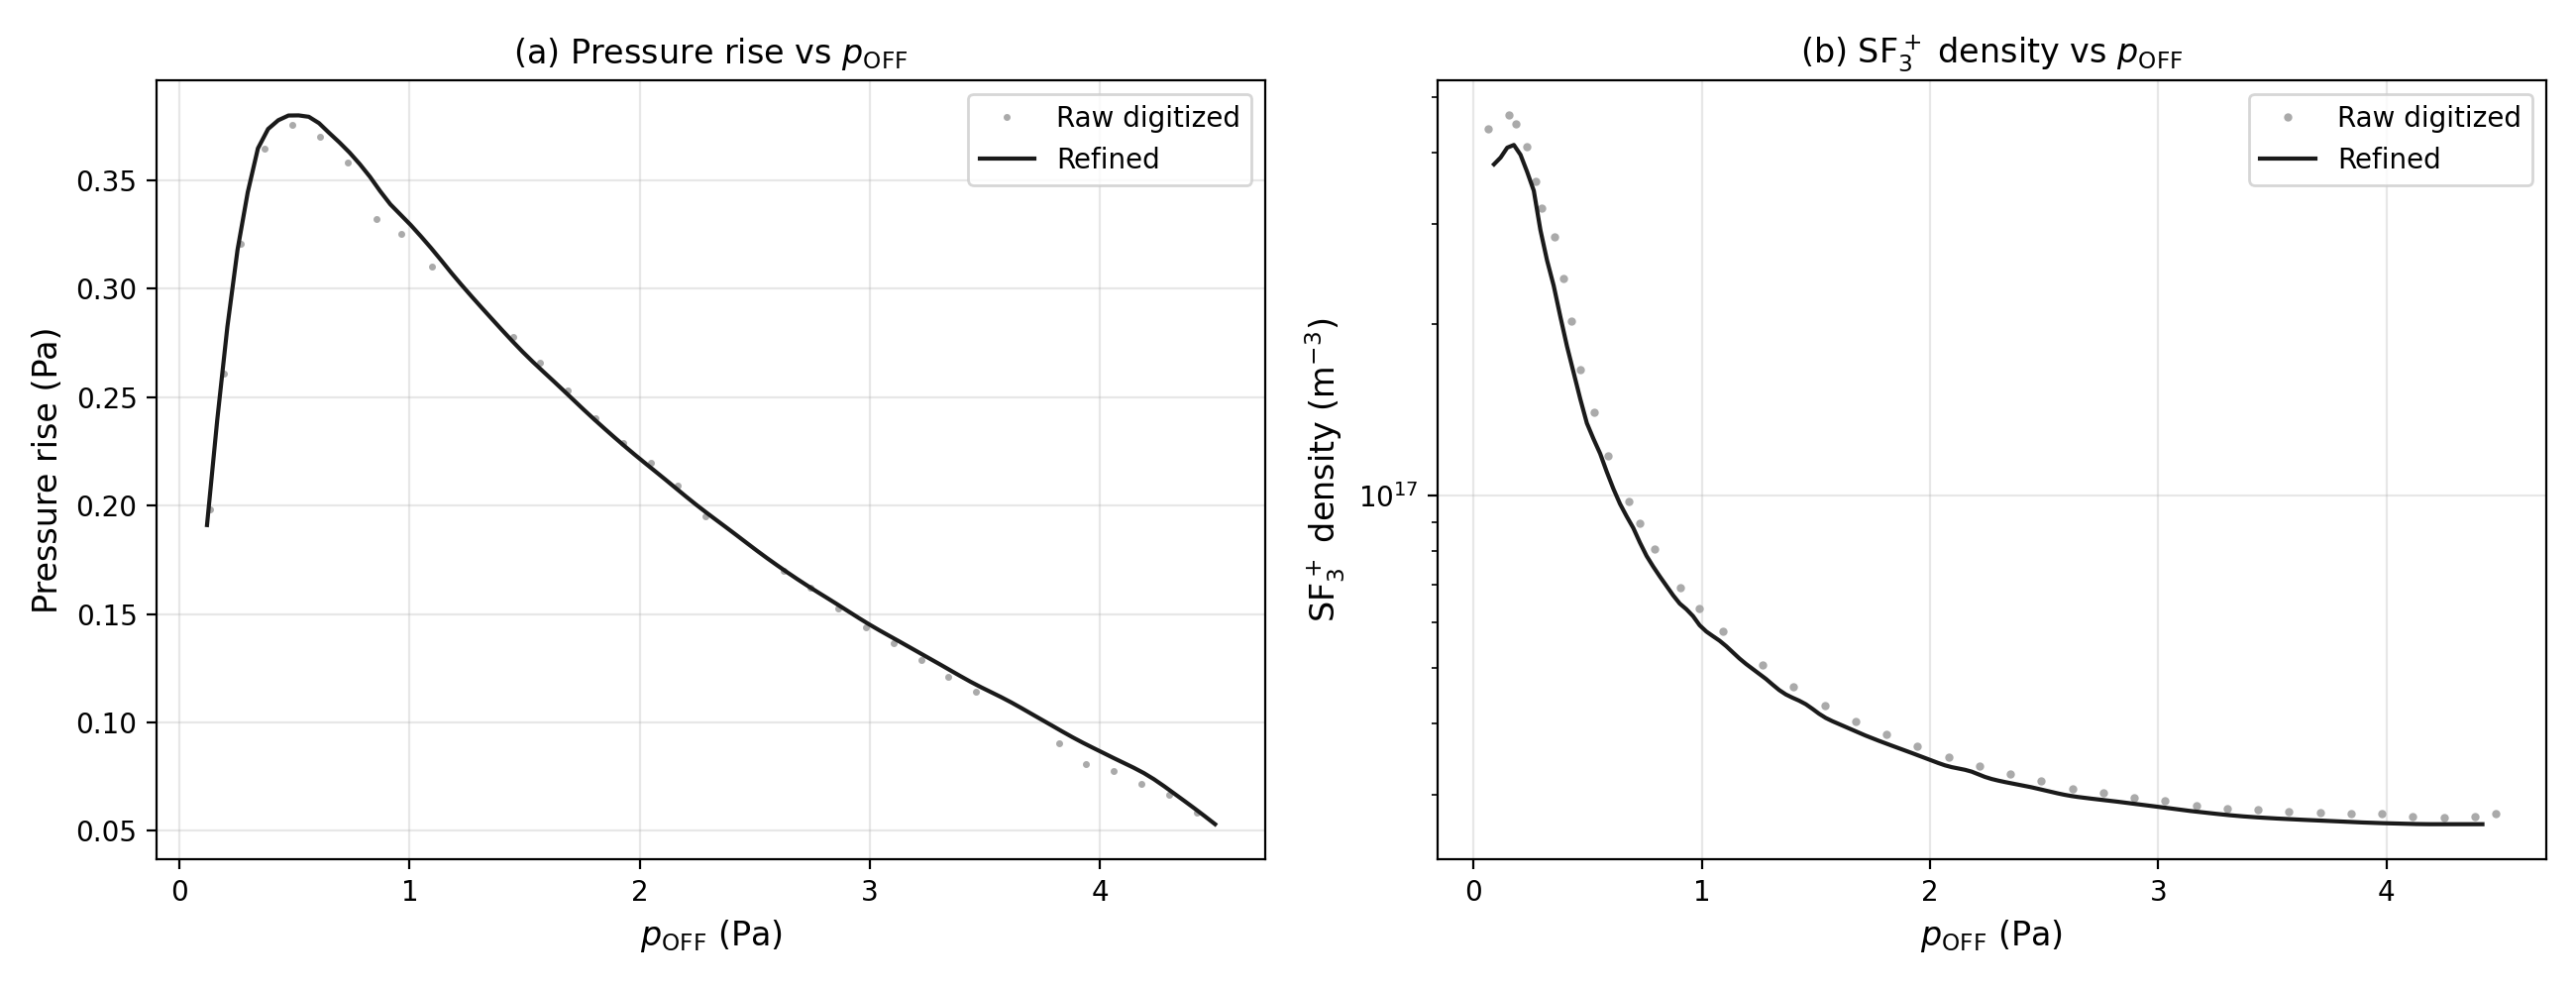
\includegraphics[width=0.95\textwidth]{raw_vs_refined.png}
\caption{Comparison of raw digitized data (grey dots) with the refined benchmark curves (black lines) for (a)~pressure rise vs $p_\text{OFF}$ and (b)~SF$_3^+$ density vs $p_\text{OFF}$.  The refinement removes digitization artefacts while preserving the underlying trends.}
\label{fig:rawvsrefined}
\end{figure}

Extraction uncertainty on logarithmic axes is estimated at $\pm0.2$~decades ($\pm60\%$).  This must be considered when interpreting discrepancies smaller than a factor of~2.

%======================================================================
\section{Results: Model Overview}
\label{sec:pure_overview}
%======================================================================

Before comparing with published data, the model's internal consistency is verified through comprehensive species density plots across both operating parameters.

\begin{figure}[H]
\centering
\begin{subfigure}[t]{0.48\textwidth}
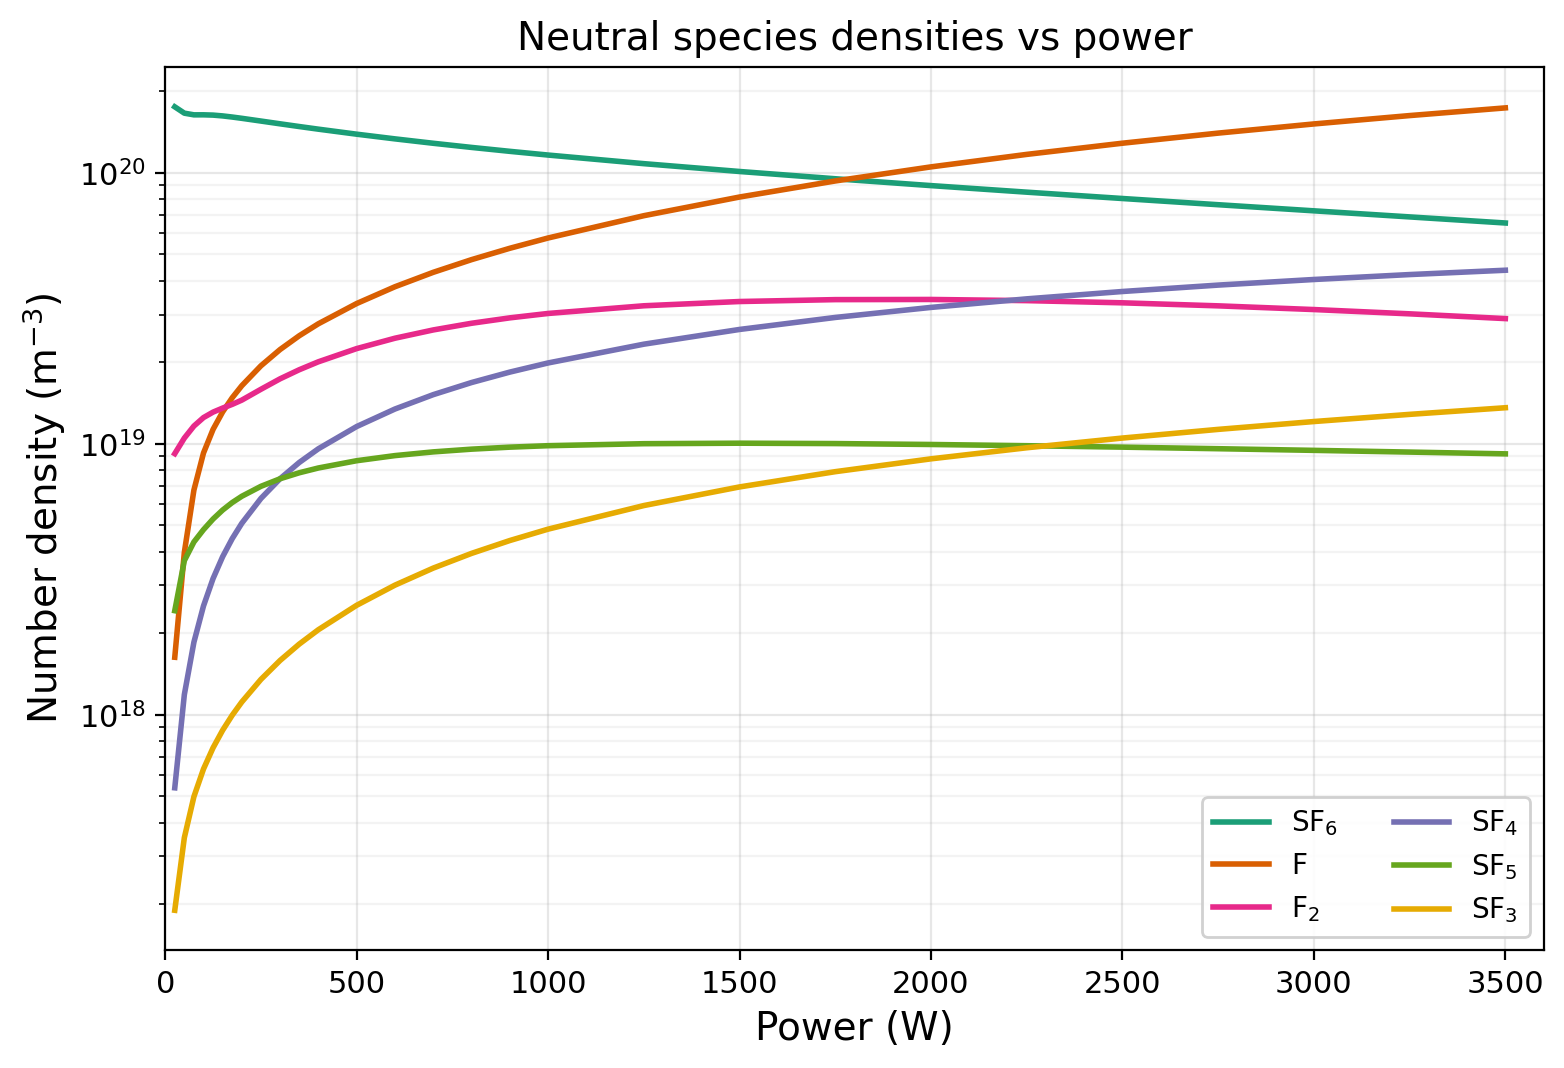
\includegraphics[width=\textwidth]{overview_neutrals_vs_power.png}
\caption{Neutral species vs power.  SF$_6$ depletes while F accumulates.  F and SF$_6$ cross near \SI{2000}{\watt}.  SF$_5$ is buffered by the Troe recombination G35.}
\label{fig:overview_neut_power}
\end{subfigure}\hfill
\begin{subfigure}[t]{0.48\textwidth}
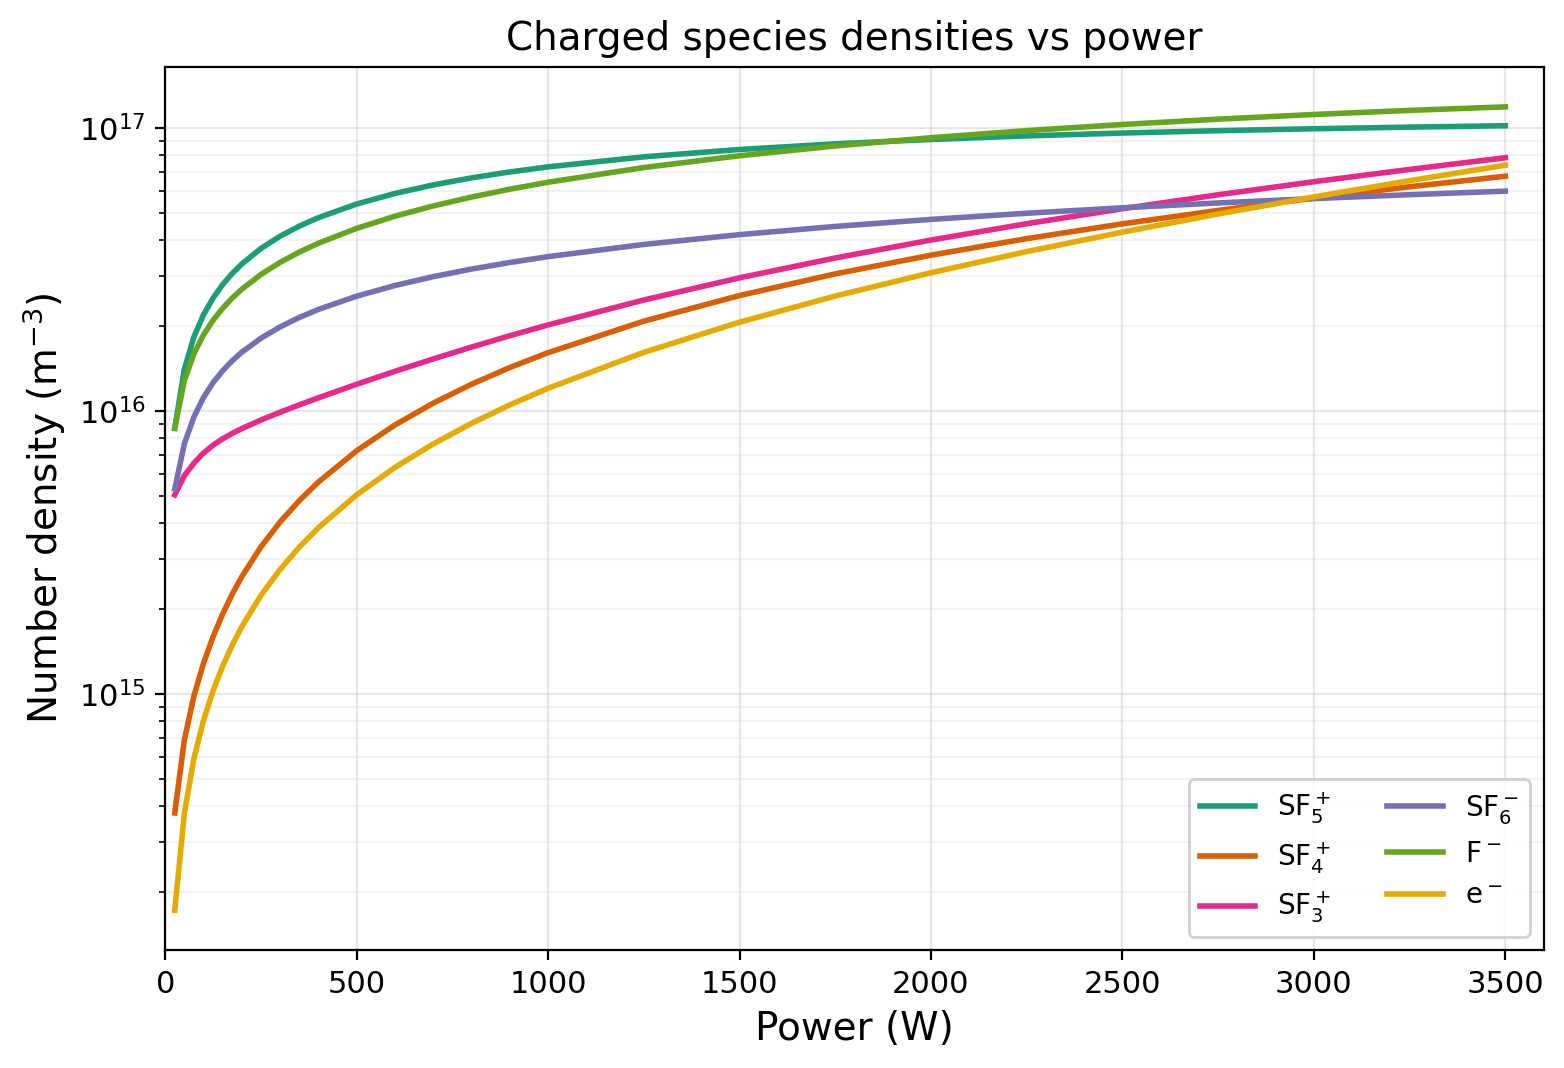
\includegraphics[width=\textwidth]{overview_charged_vs_power.png}
\caption{Charged species vs power.  SF$_5^+$ dominates.  F$^-$ and SF$_6^-$ are comparable.  $n_e$ rises monotonically with power.}
\label{fig:overview_chg_power}
\end{subfigure}
\caption{Model species densities vs power ($p_\text{OFF}=\SI{0.921}{\pascal}$).}
\label{fig:overview_power}
\end{figure}

\begin{figure}[H]
\centering
\begin{subfigure}[t]{0.48\textwidth}
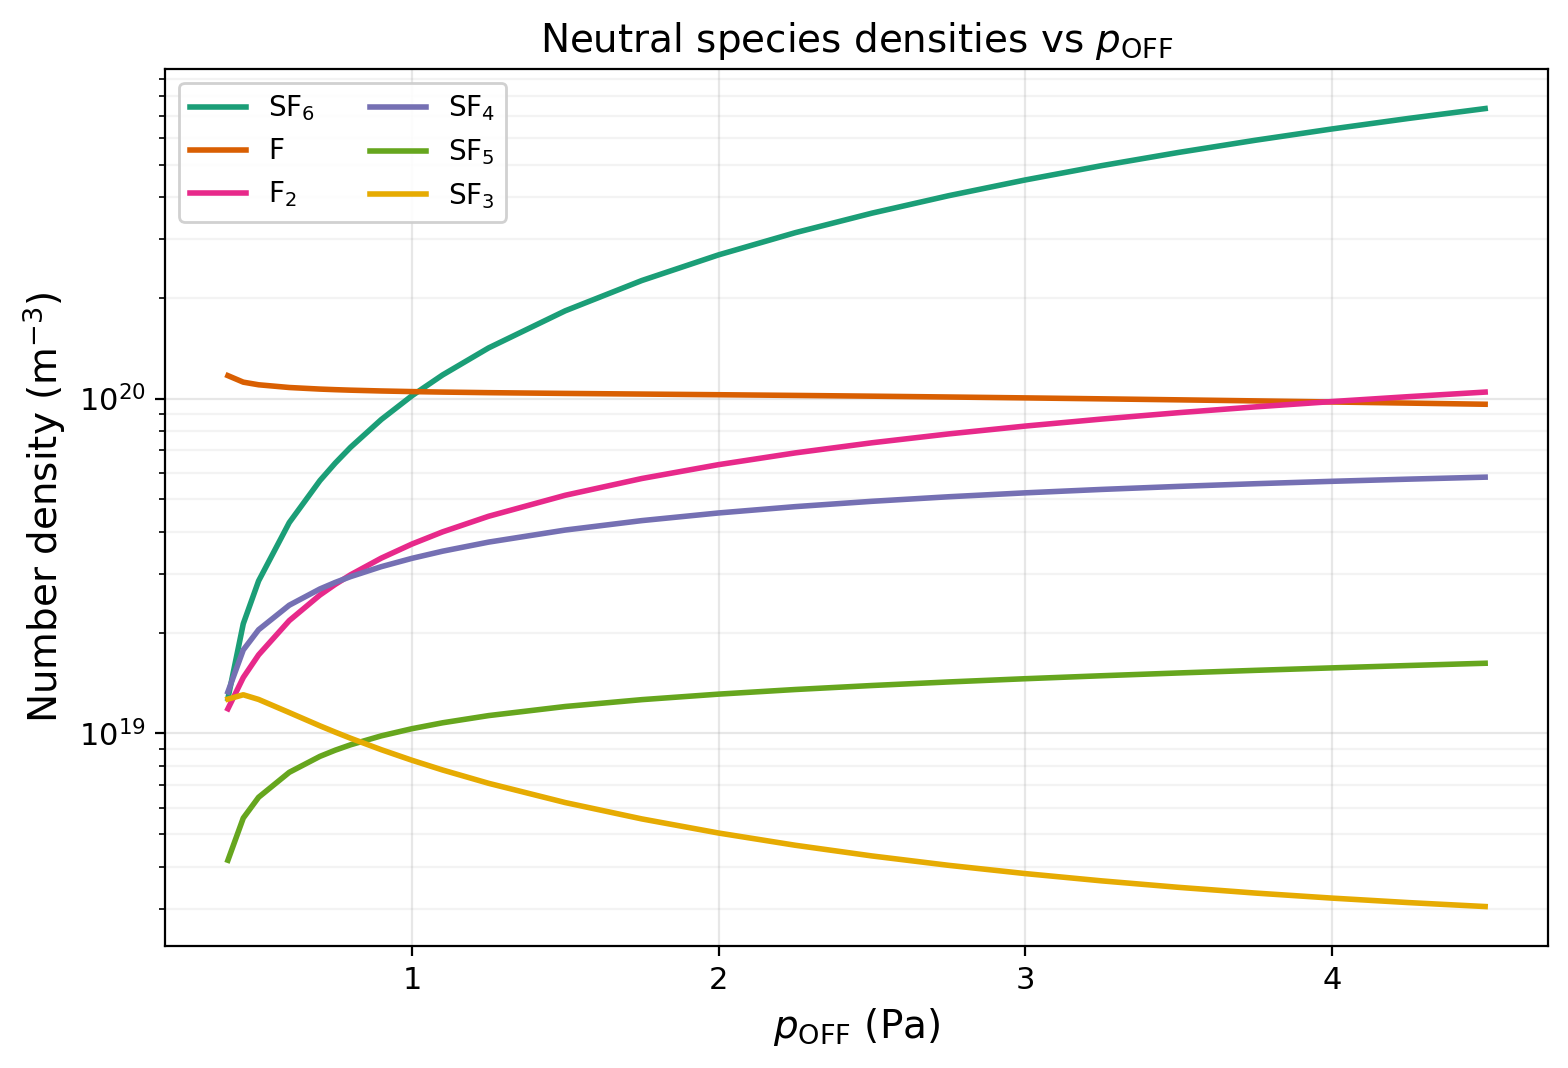
\includegraphics[width=\textwidth]{overview_neutrals_vs_poff.png}
\caption{Neutral species vs $p_\text{OFF}$.  SF$_6$ increases steeply.  F rises then plateaus.  SF$_4$ and SF$_5$ are relatively flat.}
\label{fig:overview_neut_poff}
\end{subfigure}\hfill
\begin{subfigure}[t]{0.48\textwidth}
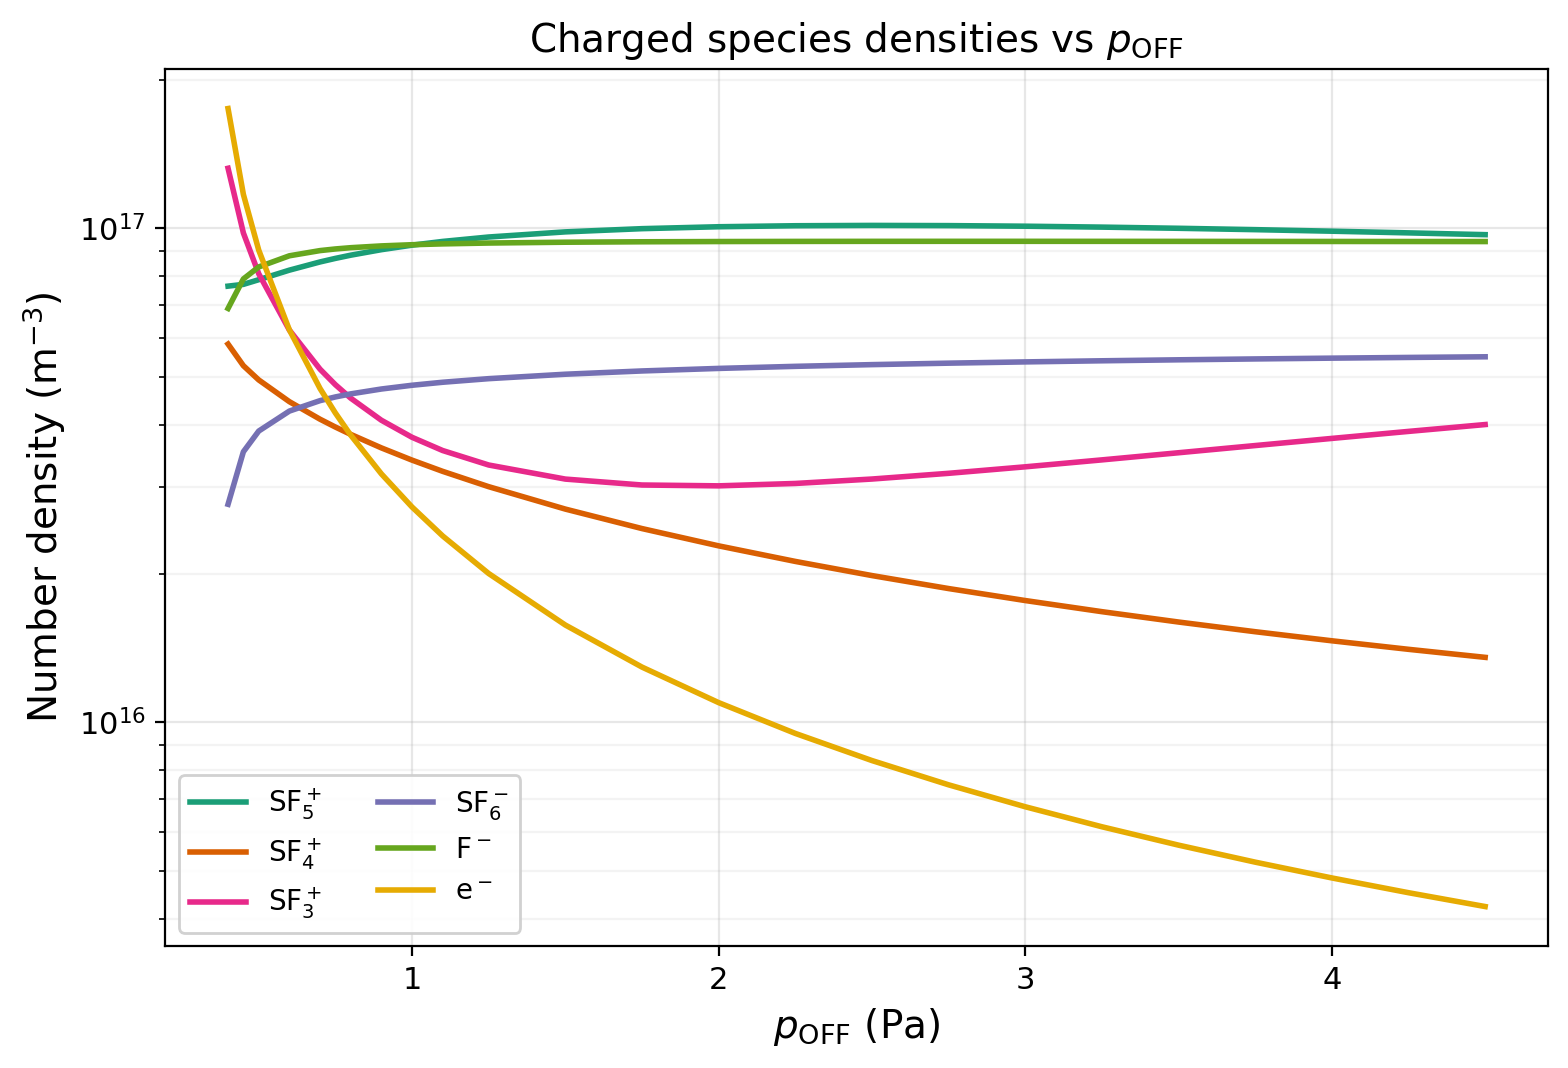
\includegraphics[width=\textwidth]{overview_charged_vs_poff.png}
\caption{Charged species vs $p_\text{OFF}$.  $n_e$ drops by $>40\times$.  Negative ions dominate at high pressure ($\alpha \gg 1$).}
\label{fig:overview_chg_poff}
\end{subfigure}
\caption{Model species densities vs $p_\text{OFF}$ ($P=\SI{2000}{\watt}$).}
\label{fig:overview_poff}
\end{figure}

%======================================================================
\section{Results: Power Sweep Comparison}
\label{sec:pure_power}
%======================================================================

\subsection{Electron Temperature and Global Quantities}
\label{sec:pure_power_global}

\begin{figure}[H]
\centering
\begin{subfigure}[t]{0.48\textwidth}
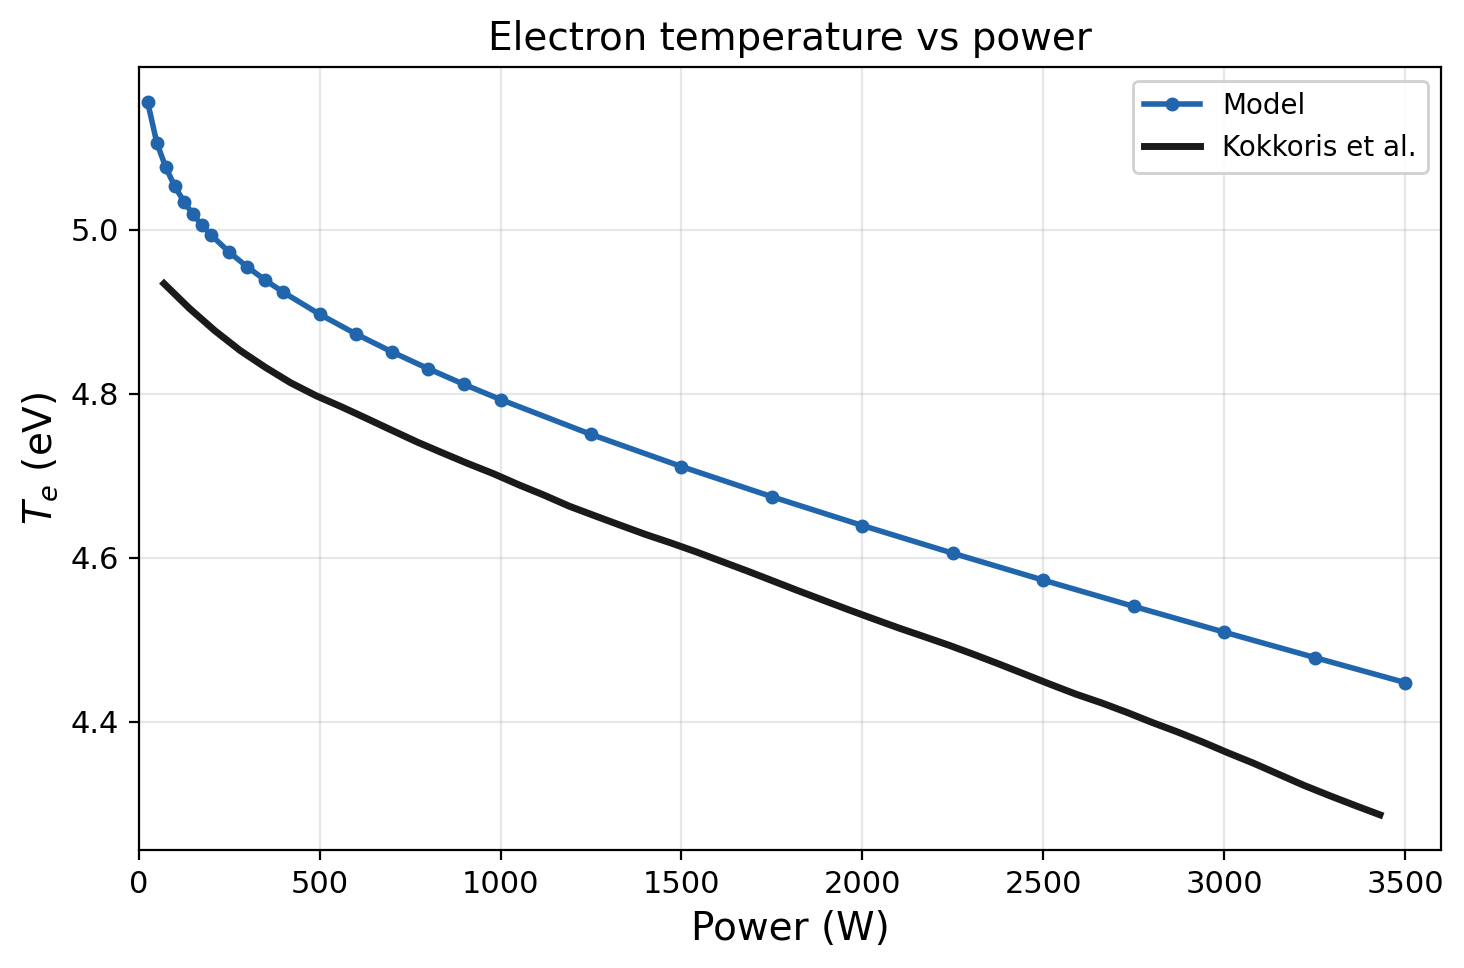
\includegraphics[width=\textwidth]{Te_vs_power.png}
\caption{$\Te$: model agrees within 2\%.  Validates the Druyvesteyn EEDF rate coefficients and ionisation--attachment balance.}
\label{fig:Te_power}
\end{subfigure}\hfill
\begin{subfigure}[t]{0.48\textwidth}
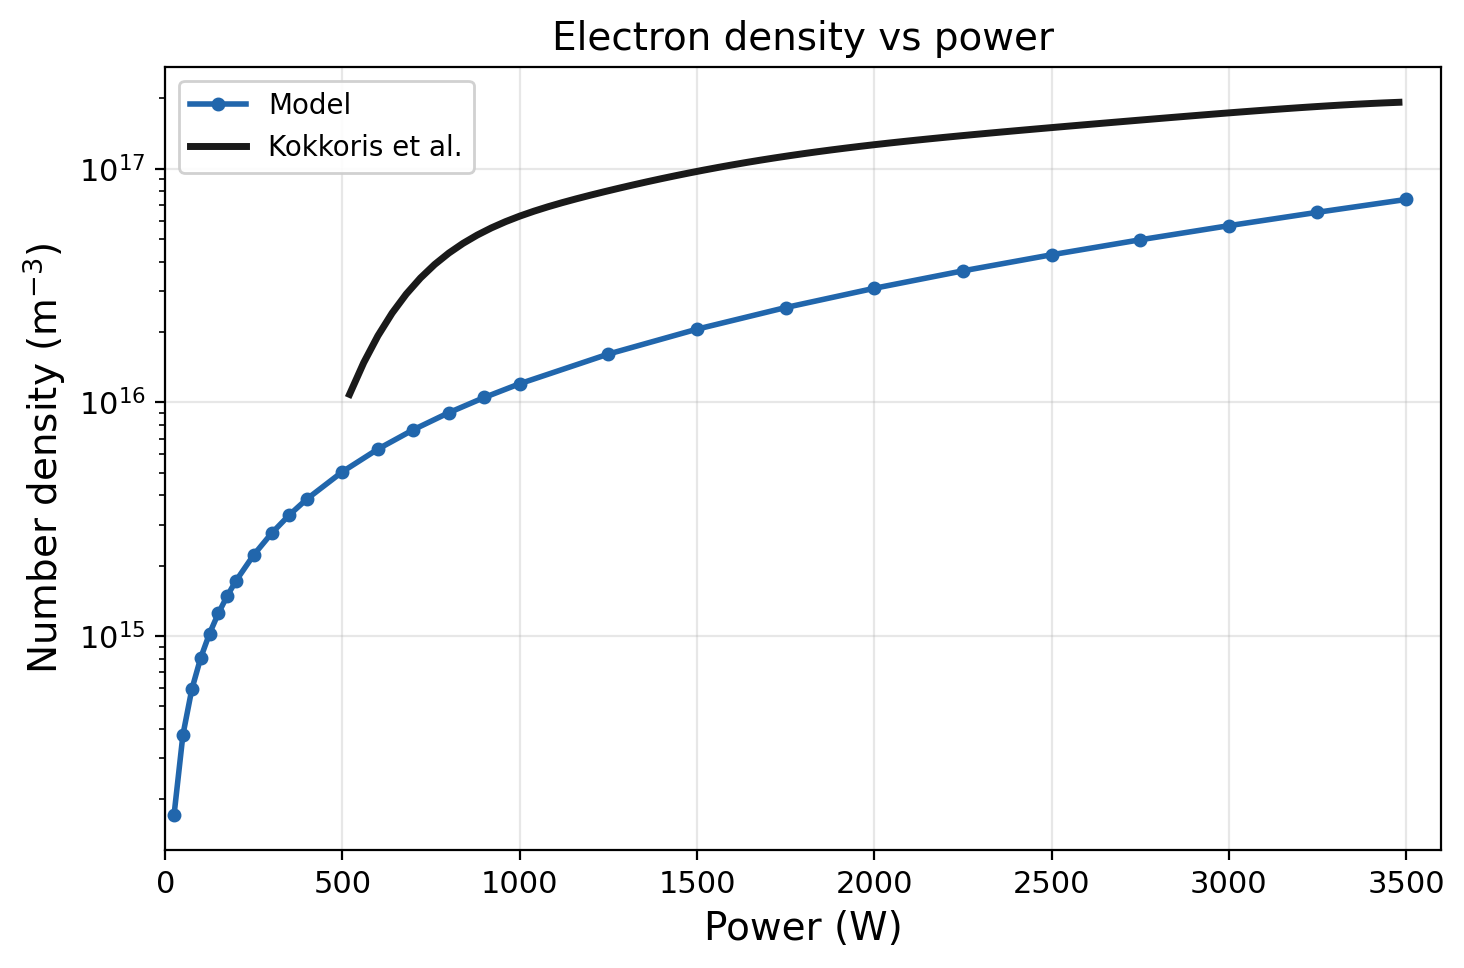
\includegraphics[width=\textwidth]{ne_vs_power.png}
\caption{$n_e$: model is ${\sim}2\times$ lower.  This is the primary discrepancy (see Section~\ref{sec:pure_discrepancy}).}
\label{fig:ne_power}
\end{subfigure}
\caption{$\Te$ and $n_e$ vs power.}
\label{fig:Te_ne_power}
\end{figure}

\begin{figure}[H]
\centering
\begin{subfigure}[t]{0.48\textwidth}
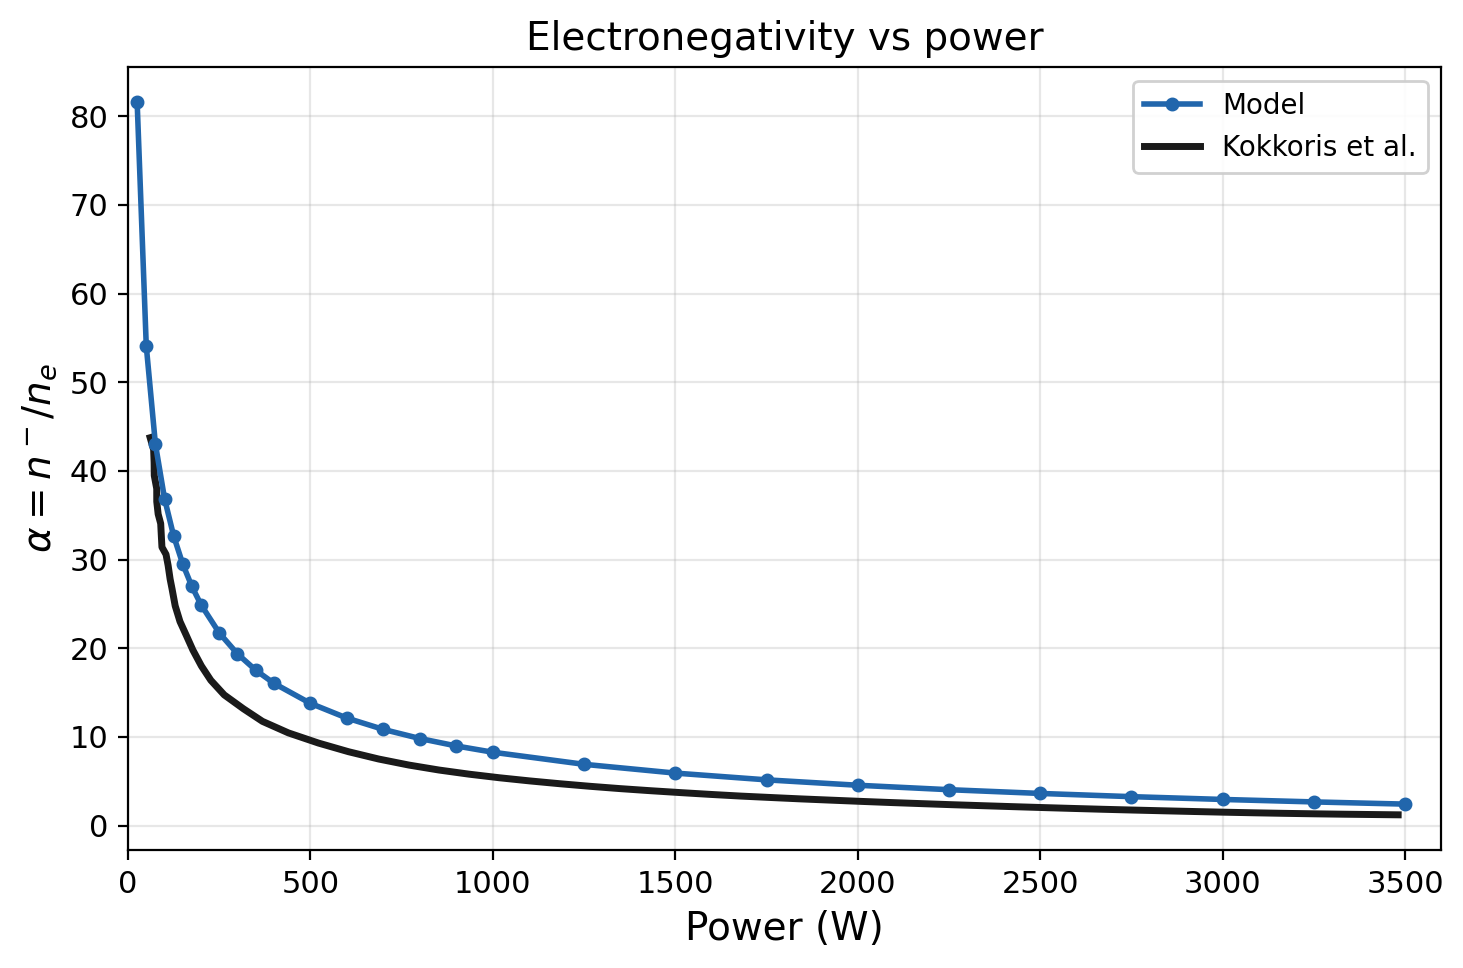
\includegraphics[width=\textwidth]{alpha_vs_power.png}
\caption{$\alpha$: model is $1.6\times$ higher, driven by the $n_e$ deficit (denominator).}
\label{fig:alpha_power}
\end{subfigure}\hfill
\begin{subfigure}[t]{0.48\textwidth}
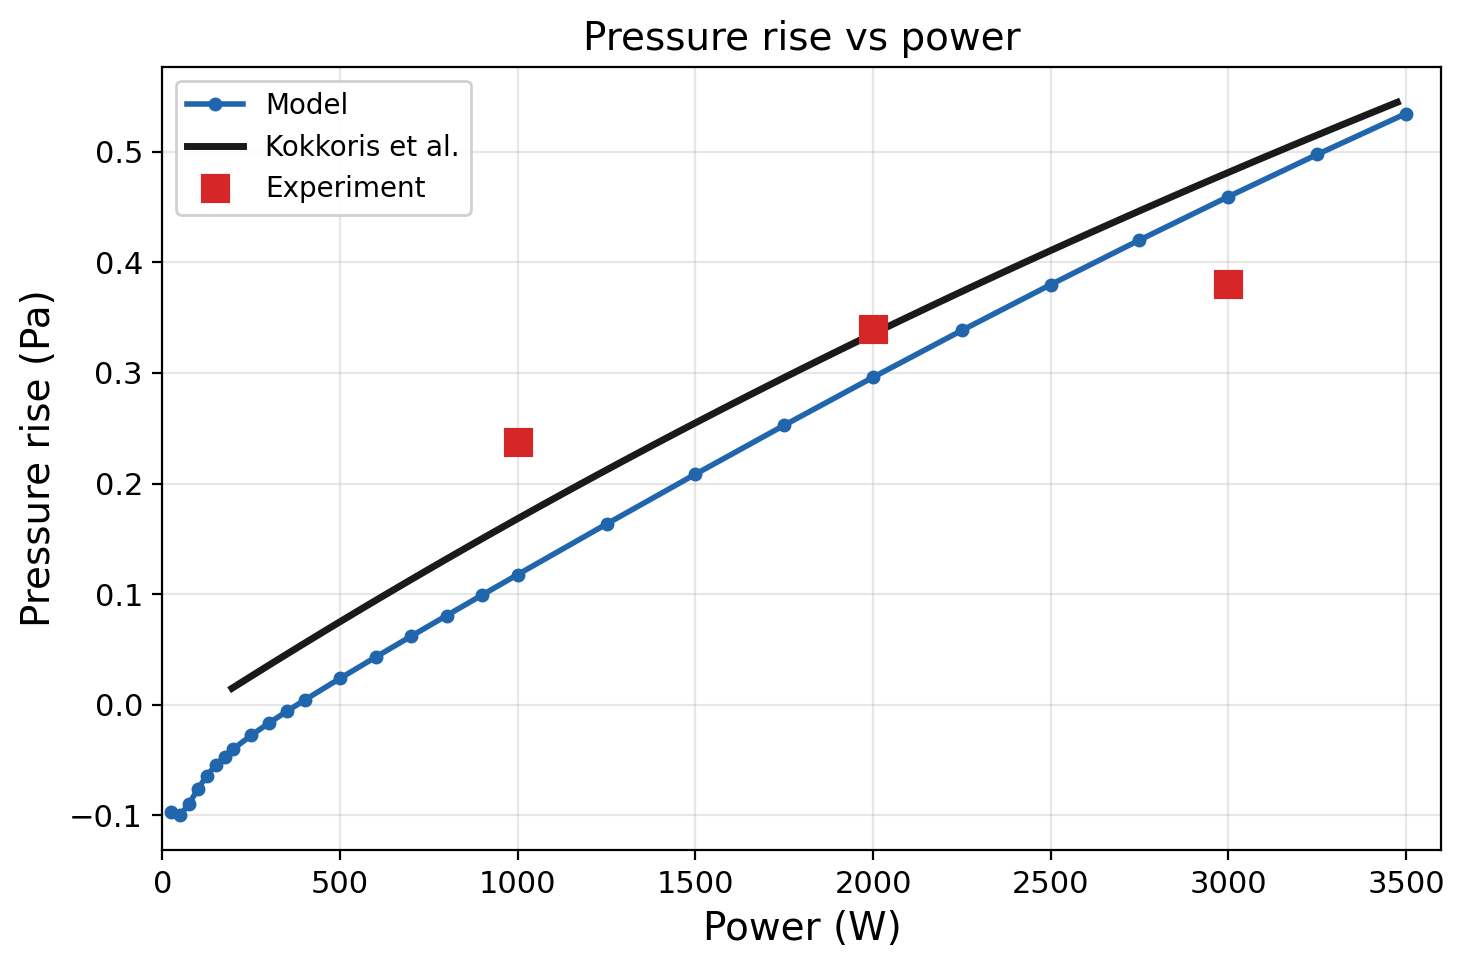
\includegraphics[width=\textwidth]{dp_vs_power.png}
\caption{Pressure rise: model tracks experimental data (squares) well.}
\label{fig:dp_power}
\end{subfigure}
\caption{$\alpha$ and $\Delta p$ vs power.}
\label{fig:alpha_dp_power}
\end{figure}

\subsection{Neutral Species}
\label{sec:pure_power_neutrals}

\begin{figure}[H]
\centering
\begin{subfigure}[t]{0.48\textwidth}
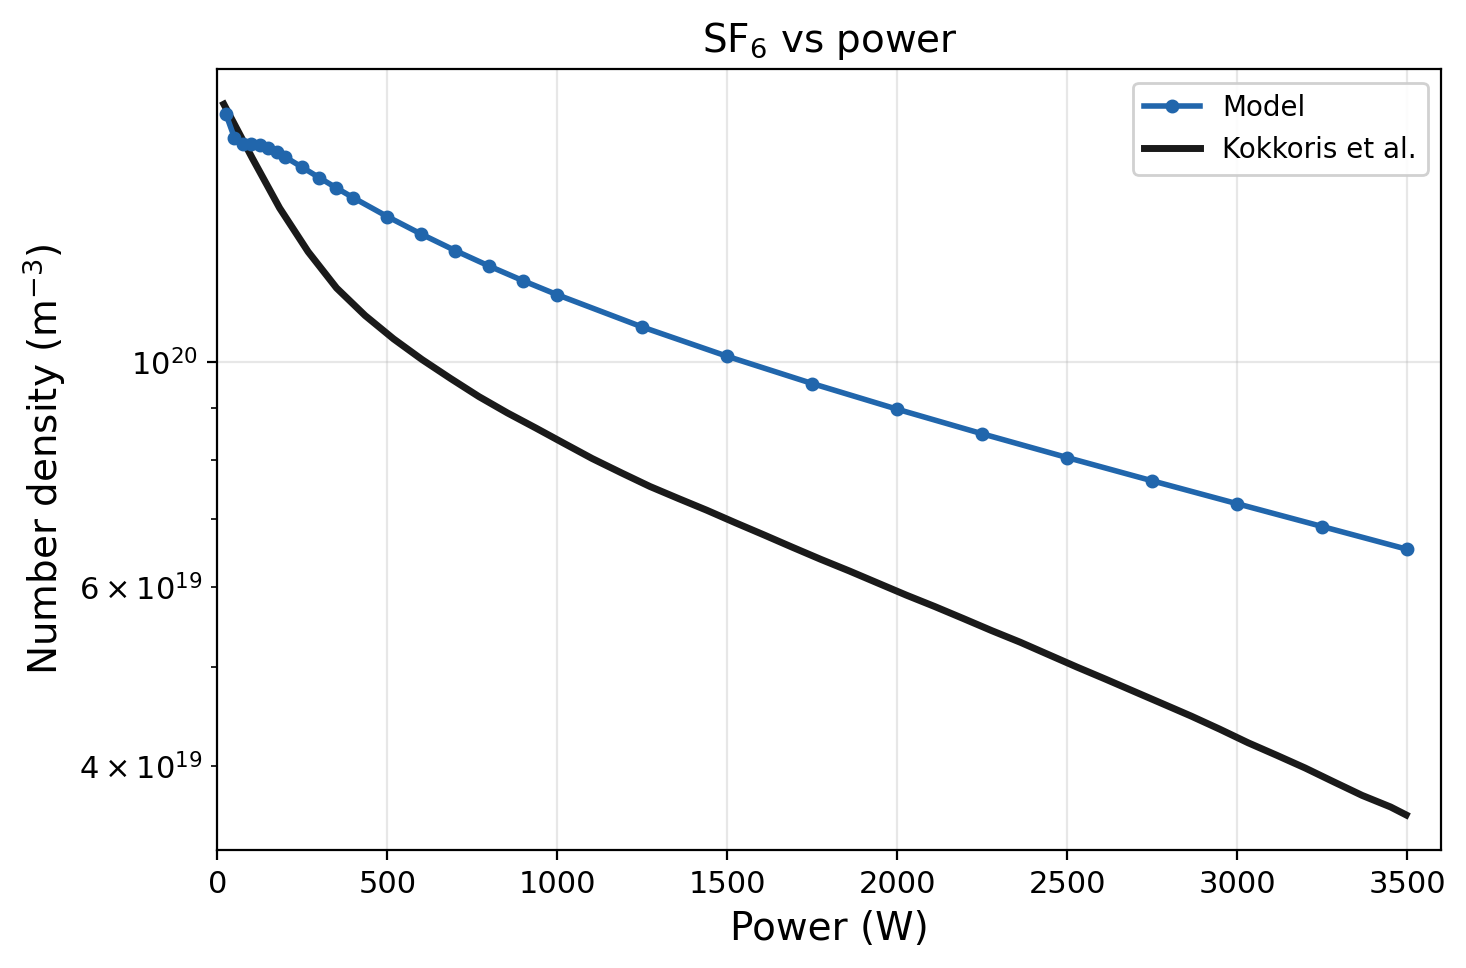
\includegraphics[width=\textwidth]{nSF6_m3_vs_power.png}
\caption{SF$_6$: $1.47\times$ higher.  Less dissociation from lower $n_e$.}
\label{fig:nSF6_power}
\end{subfigure}\hfill
\begin{subfigure}[t]{0.48\textwidth}
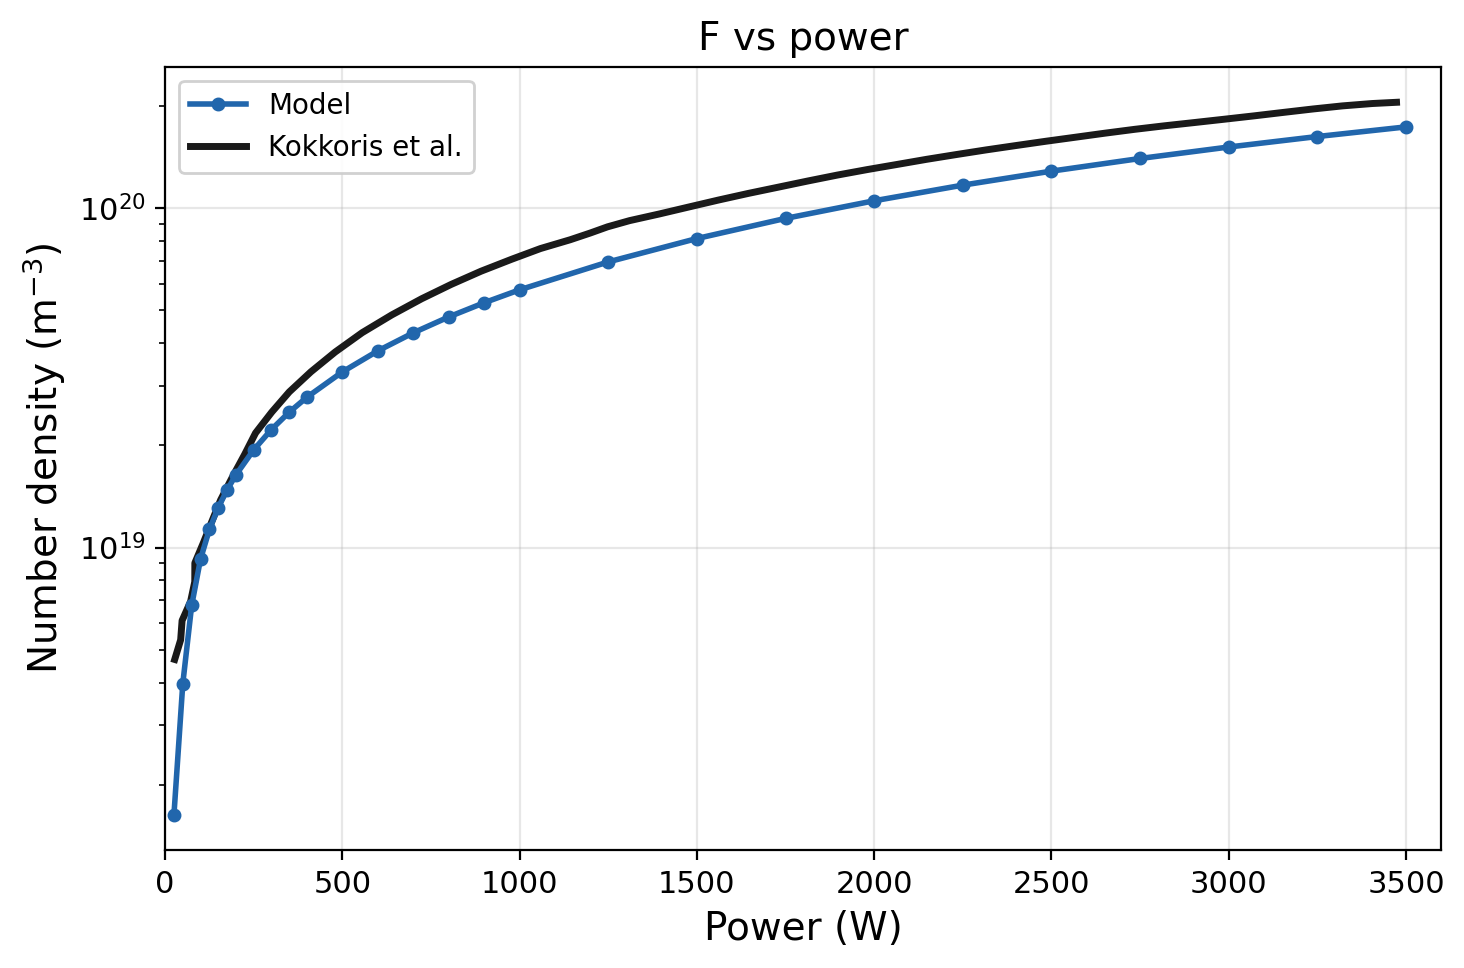
\includegraphics[width=\textwidth]{nF_m3_vs_power.png}
\caption{F: $0.81\times$.  Less production from lower dissociation rate.}
\label{fig:nF_power}
\end{subfigure}
\caption{SF$_6$ and F vs power.}
\label{fig:SF6_F_power}
\end{figure}

\begin{figure}[H]
\centering
\begin{subfigure}[t]{0.48\textwidth}
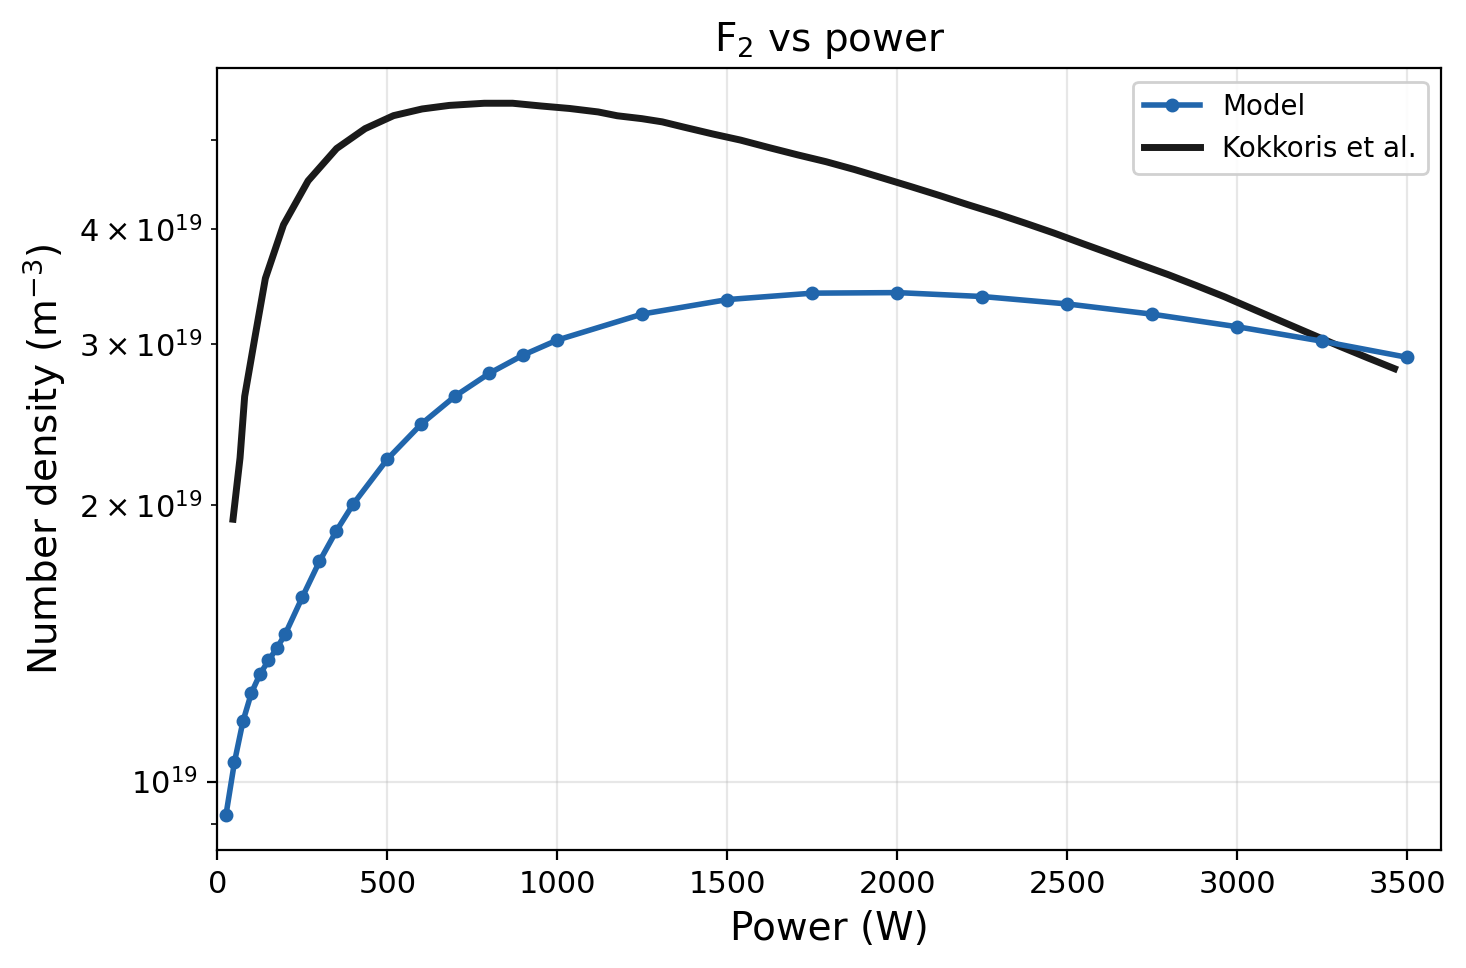
\includegraphics[width=\textwidth]{nF2_m3_vs_power.png}
\caption{F$_2$: $0.76\times$.  Produced by surface recombination of F, so inherits the F offset.}
\label{fig:nF2_power}
\end{subfigure}\hfill
\begin{subfigure}[t]{0.48\textwidth}
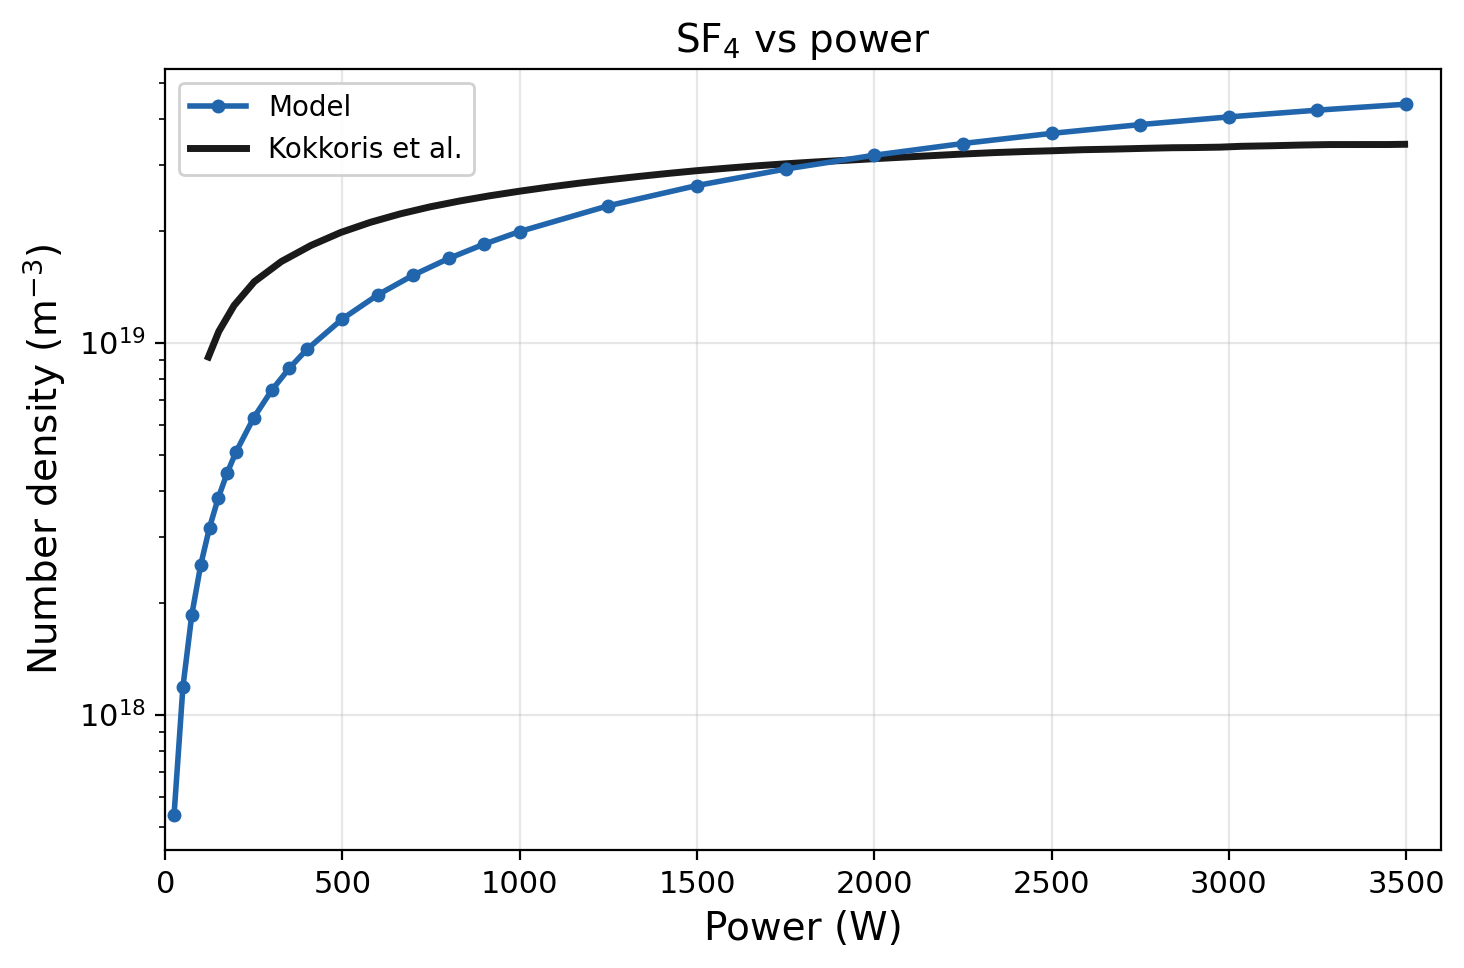
\includegraphics[width=\textwidth]{nSF4_m3_vs_power.png}
\caption{SF$_4$: $1.01\times$ --- near-perfect.  Stabilised by multiple production pathways.}
\label{fig:nSF4_power}
\end{subfigure}
\caption{F$_2$ and SF$_4$ vs power.}
\label{fig:F2_SF4_power}
\end{figure}

\begin{figure}[H]
\centering
\begin{subfigure}[t]{0.48\textwidth}
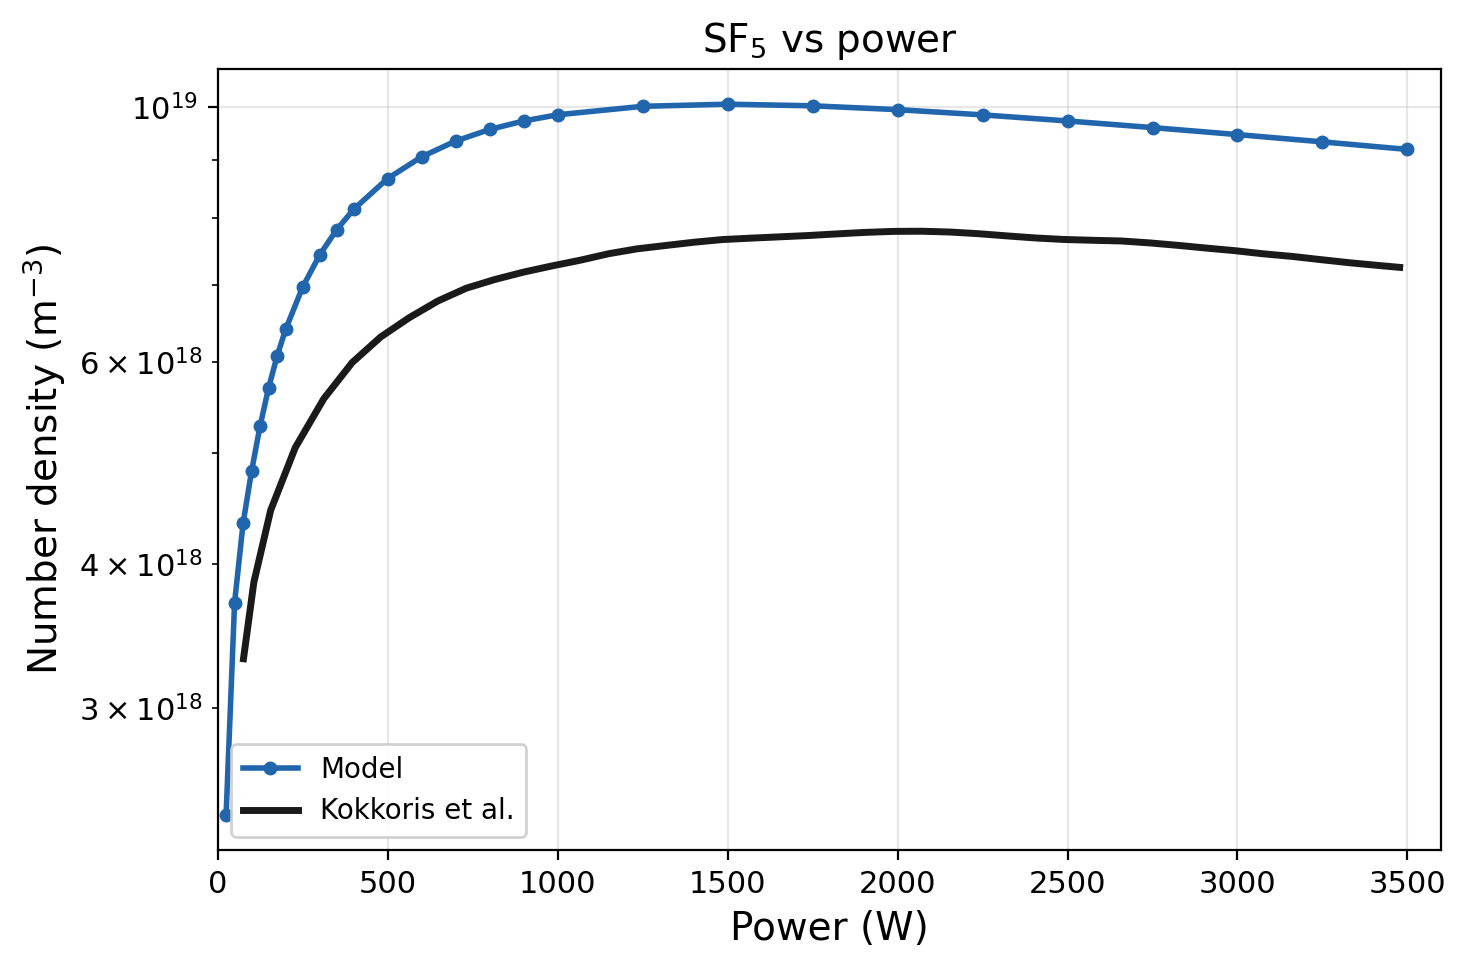
\includegraphics[width=\textwidth]{nSF5_m3_vs_power.png}
\caption{SF$_5$: $1.26\times$.  The Troe buffer (G35) keeps the profile flat.}
\label{fig:nSF5_power}
\end{subfigure}\hfill
\begin{subfigure}[t]{0.48\textwidth}
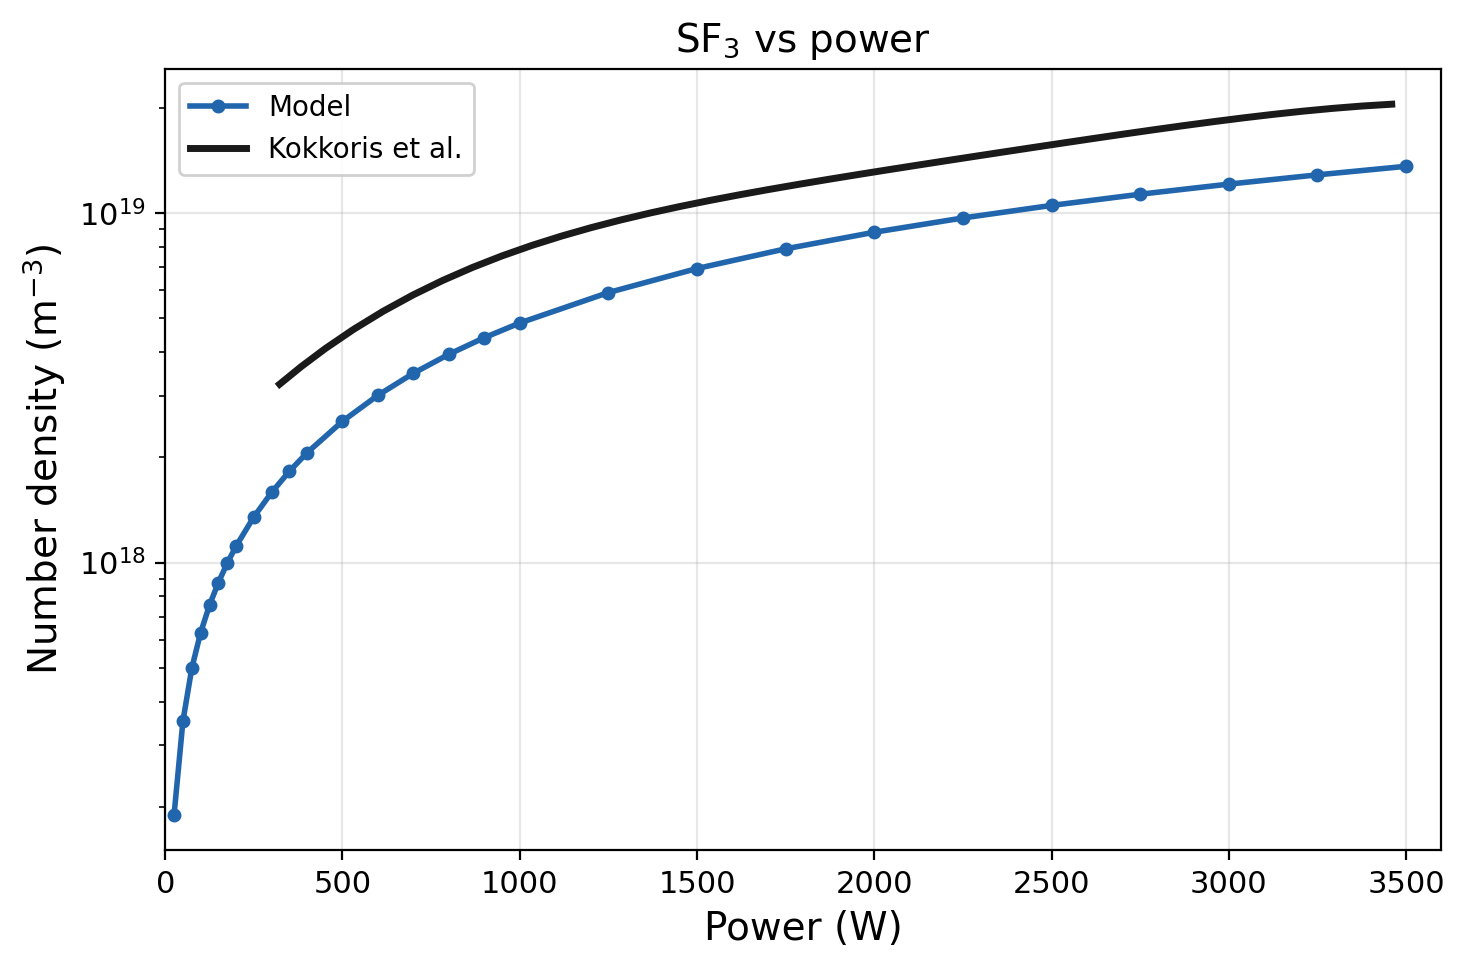
\includegraphics[width=\textwidth]{nSF3_m3_vs_power.png}
\caption{SF$_3$: $0.68\times$.  Least abundant neutral radical.}
\label{fig:nSF3_power}
\end{subfigure}
\caption{SF$_5$ and SF$_3$ vs power.}
\label{fig:SF5_SF3_power}
\end{figure}

\subsection{Charged Species}
\label{sec:pure_power_charged}

\begin{figure}[H]
\centering
\begin{subfigure}[t]{0.48\textwidth}
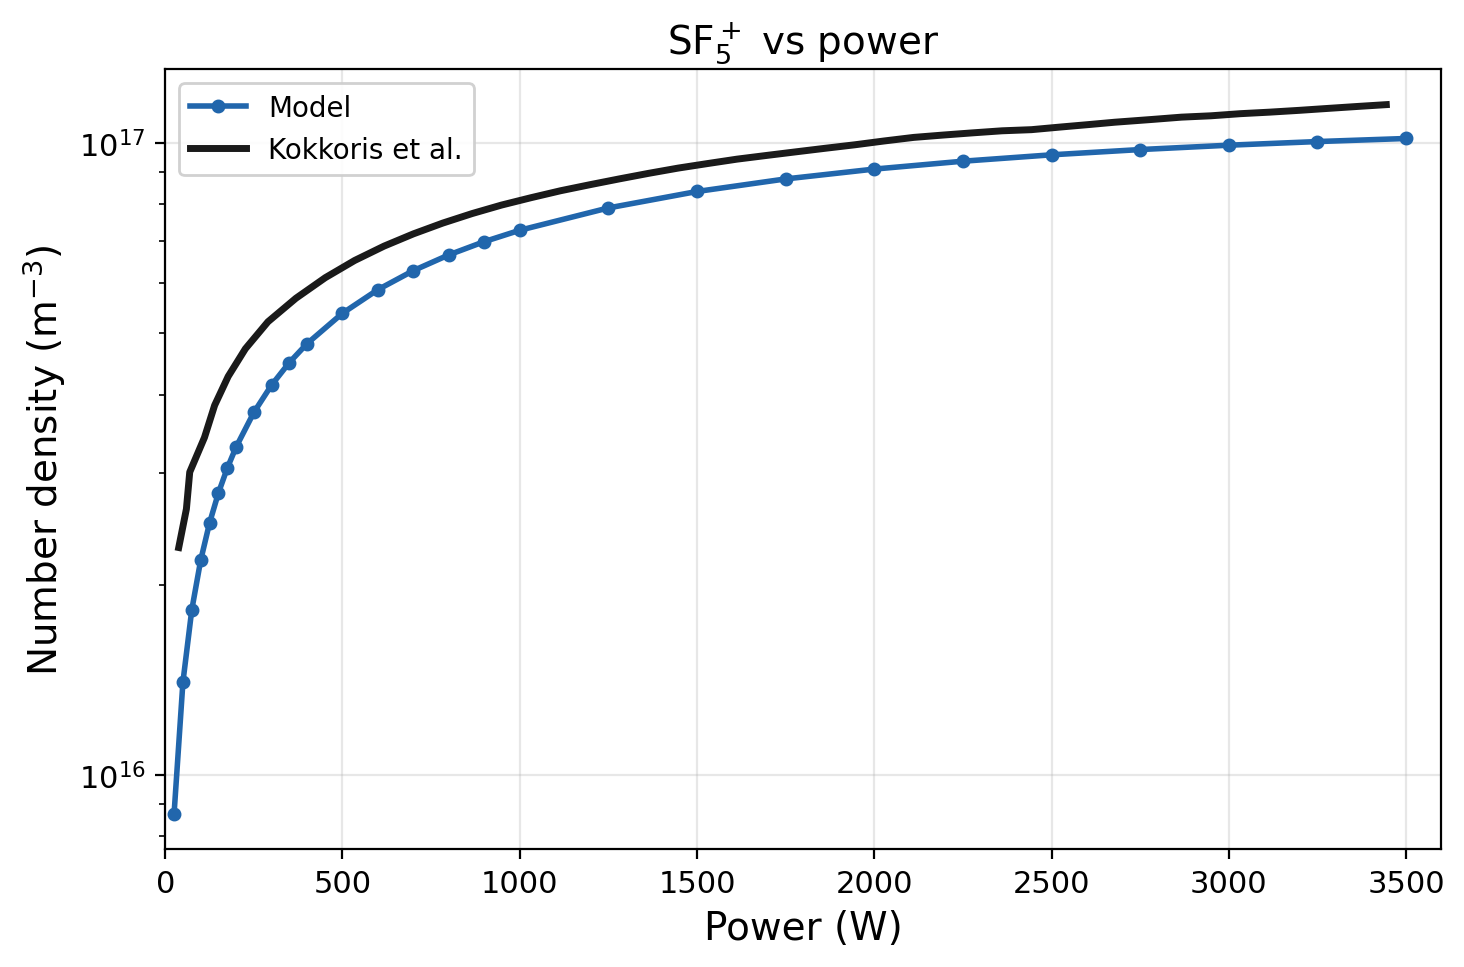
\includegraphics[width=\textwidth]{nSF5p_m3_vs_power.png}
\caption{SF$_5^+$: $0.91\times$.  Dominant positive ion.}
\label{fig:nSF5p_power}
\end{subfigure}\hfill
\begin{subfigure}[t]{0.48\textwidth}
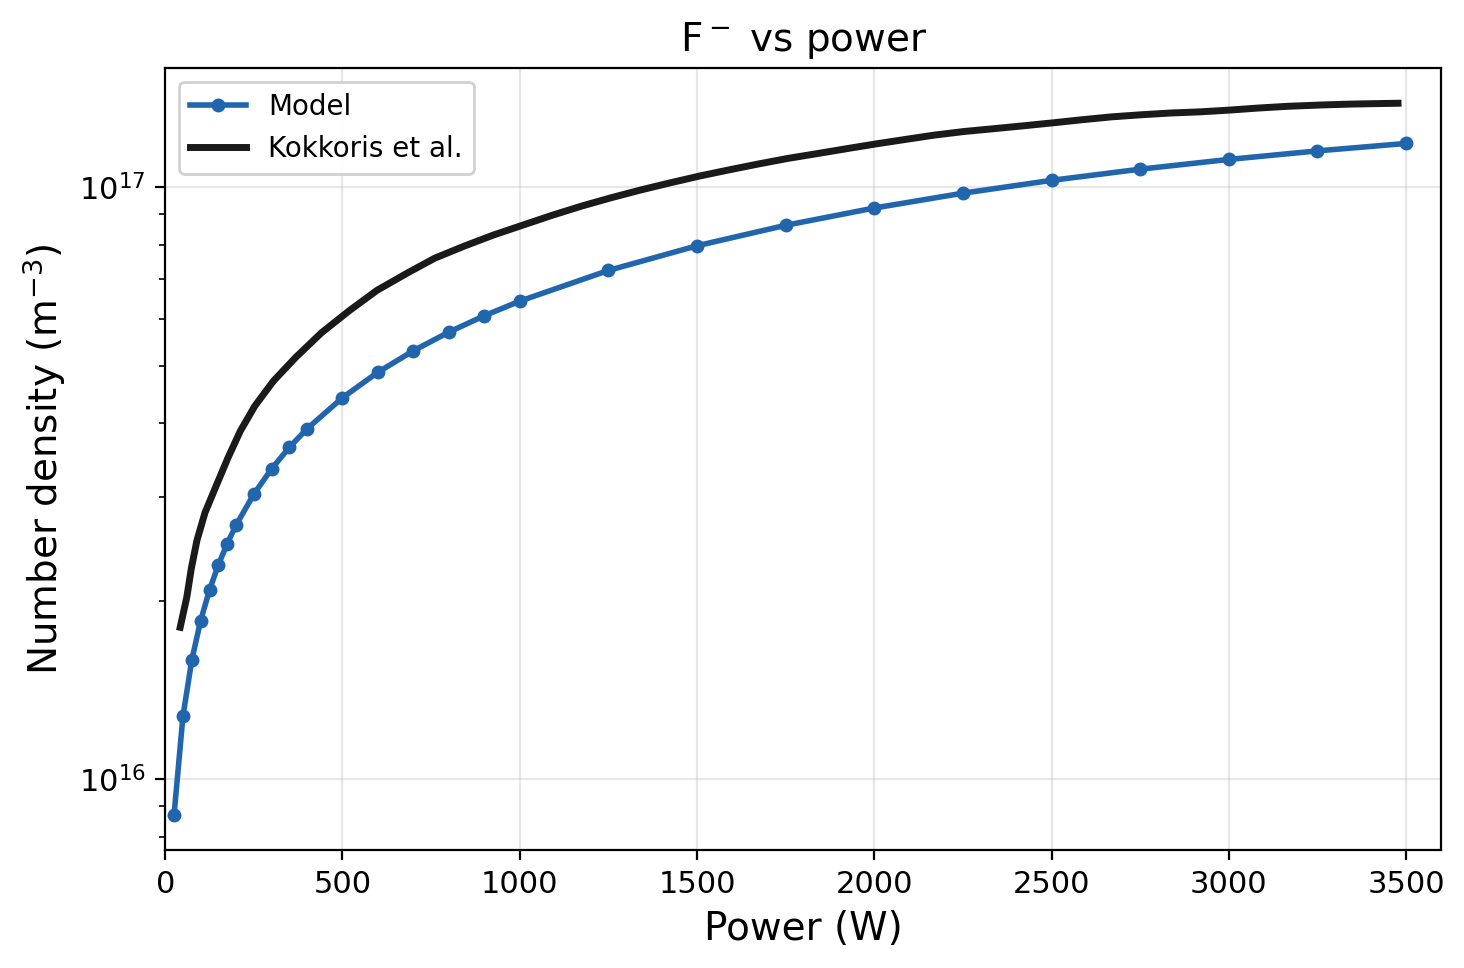
\includegraphics[width=\textwidth]{nFm_m3_vs_power.png}
\caption{F$^-$: $0.78\times$.  Dominant negative ion.}
\label{fig:nFm_power}
\end{subfigure}
\caption{Dominant ions vs power.}
\label{fig:dom_ions_power}
\end{figure}

\begin{figure}[H]
\centering
\begin{subfigure}[t]{0.48\textwidth}
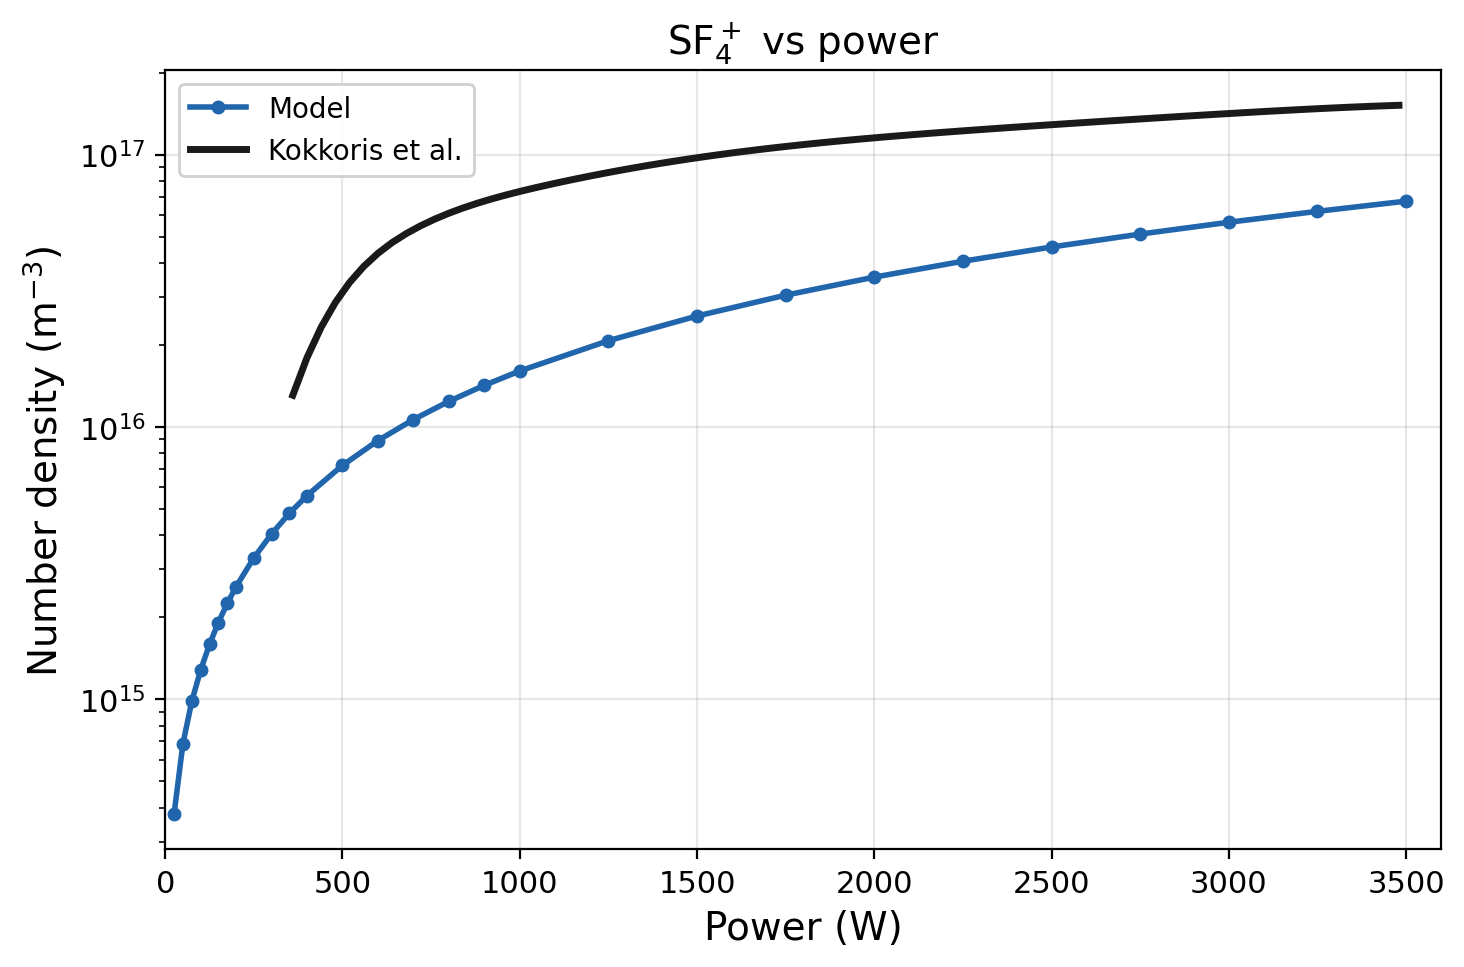
\includegraphics[width=\textwidth]{nSF4p_m3_vs_power.png}
\caption{SF$_4^+$: secondary positive ion.}
\label{fig:nSF4p_power}
\end{subfigure}\hfill
\begin{subfigure}[t]{0.48\textwidth}
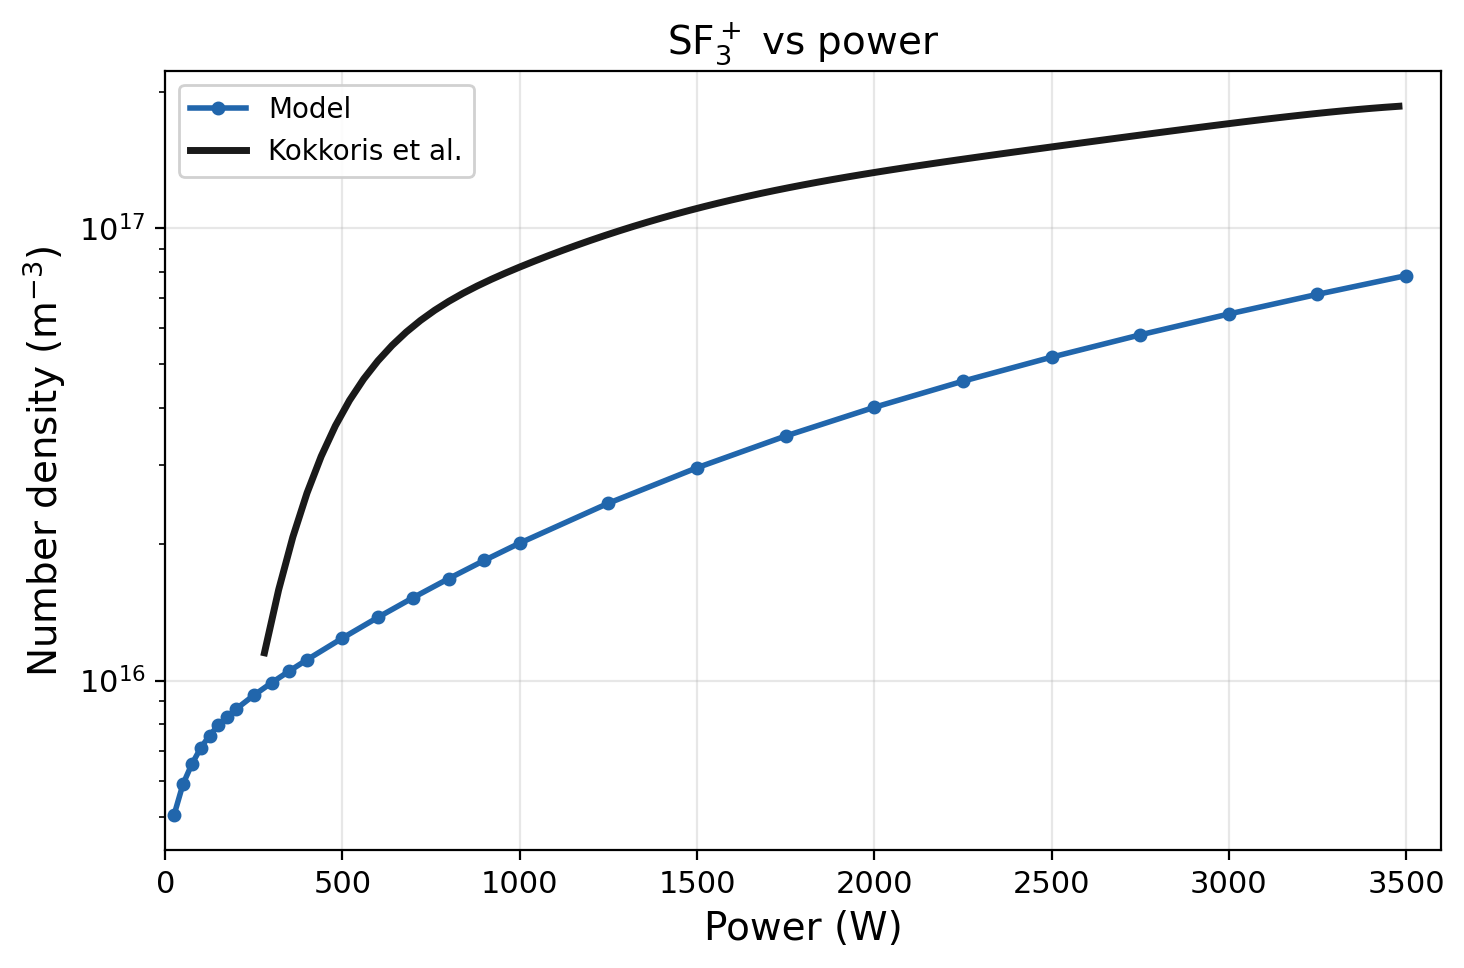
\includegraphics[width=\textwidth]{nSF3p_m3_vs_power.png}
\caption{SF$_3^+$: secondary positive ion.}
\label{fig:nSF3p_power}
\end{subfigure}
\caption{Secondary ions vs power.}
\label{fig:sec_ions_power}
\end{figure}

\begin{figure}[H]
\centering
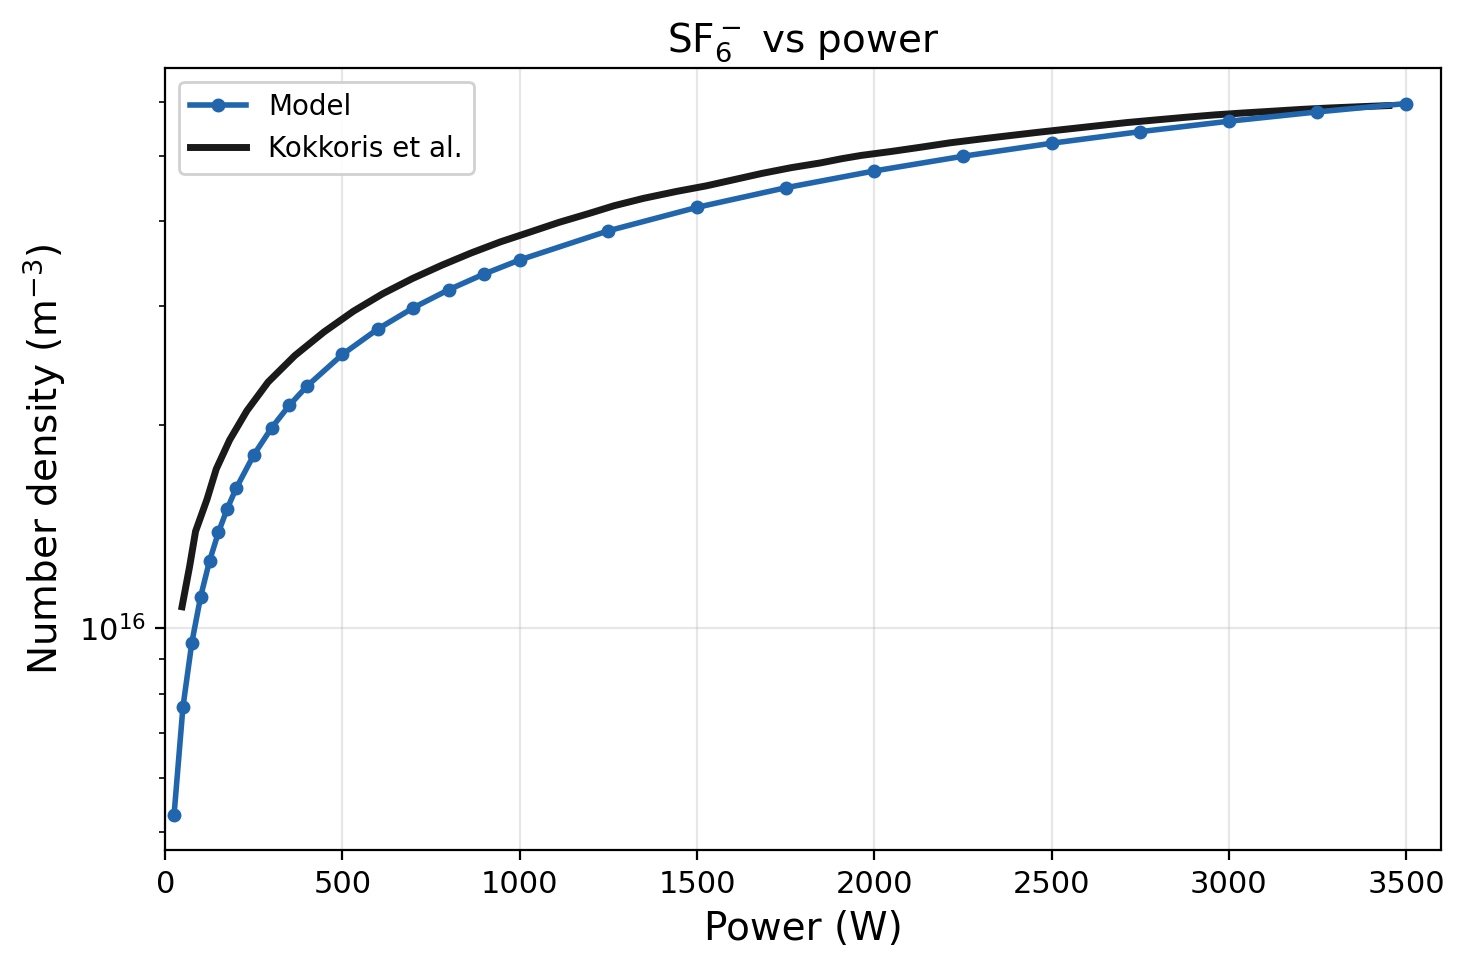
\includegraphics[width=0.55\textwidth]{nSF6m_m3_vs_power.png}
\caption{SF$_6^-$: $0.94\times$ --- excellent.  Produced by non-dissociative attachment (G18).}
\label{fig:nSF6m_power}
\end{figure}

\subsection{F Density with Experimental Data}
\label{sec:pure_power_Fexp}

\begin{figure}[H]
\centering
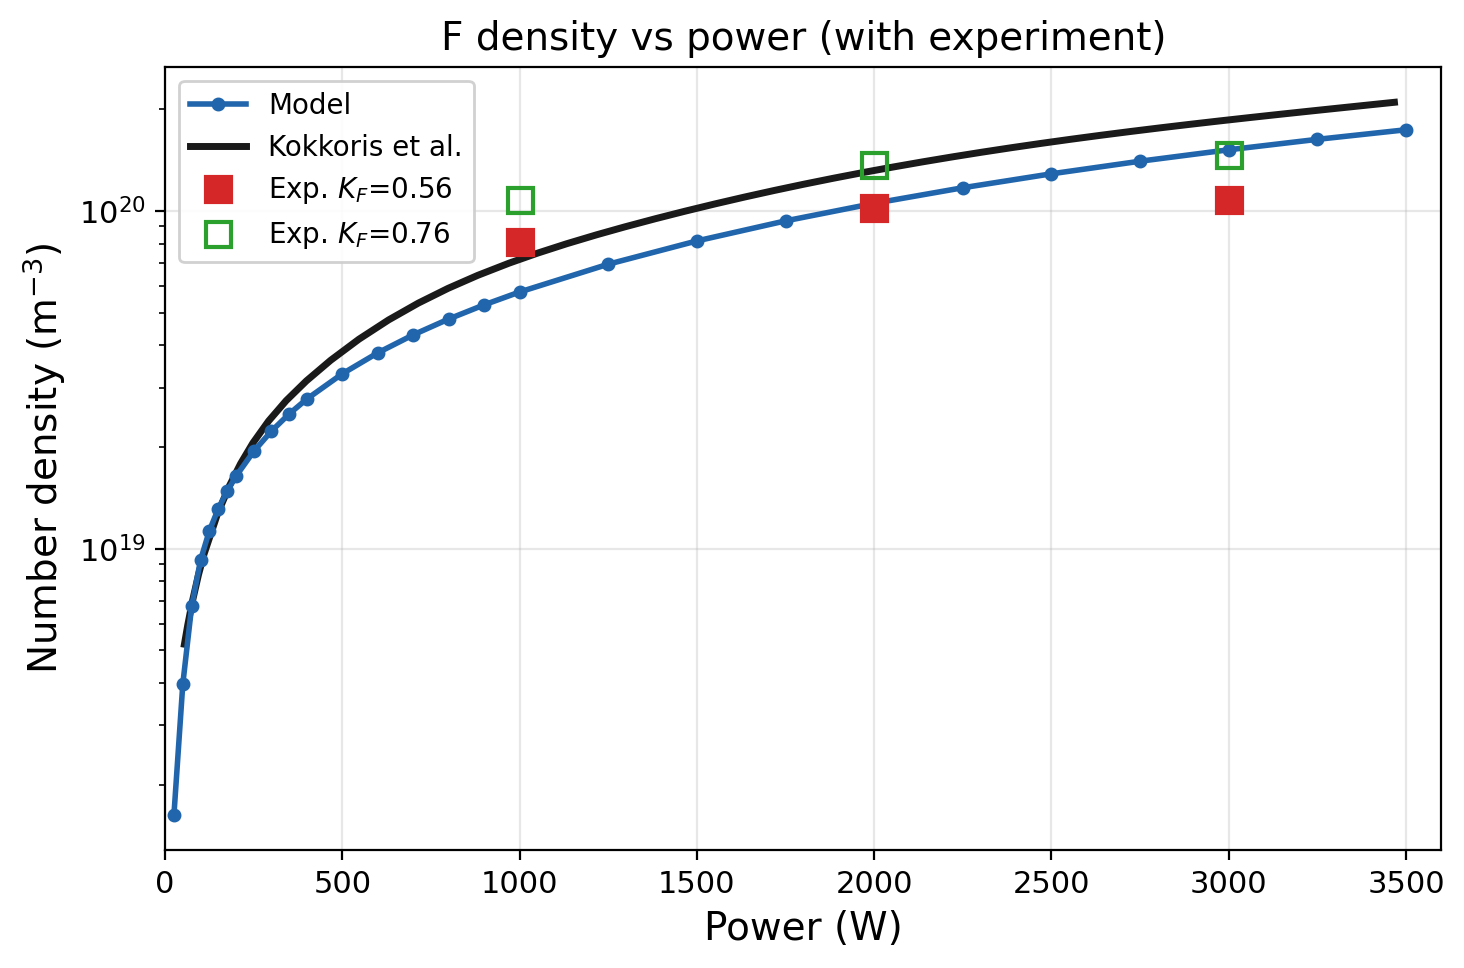
\includegraphics[width=0.65\textwidth]{nF_with_exp_vs_power.png}
\caption{F density with experimental actinometry data.  The model sits between the two $K_F$ calibration values, consistent with the ${\sim}2\times$ experimental uncertainty.}
\label{fig:nF_exp_power}
\end{figure}

%======================================================================
\section{Results: Pressure Sweep Comparison}
\label{sec:pure_pressure}
%======================================================================

\subsection{Electron Temperature and Global Quantities}
\label{sec:pure_poff_global}

\begin{figure}[H]
\centering
\begin{subfigure}[t]{0.48\textwidth}
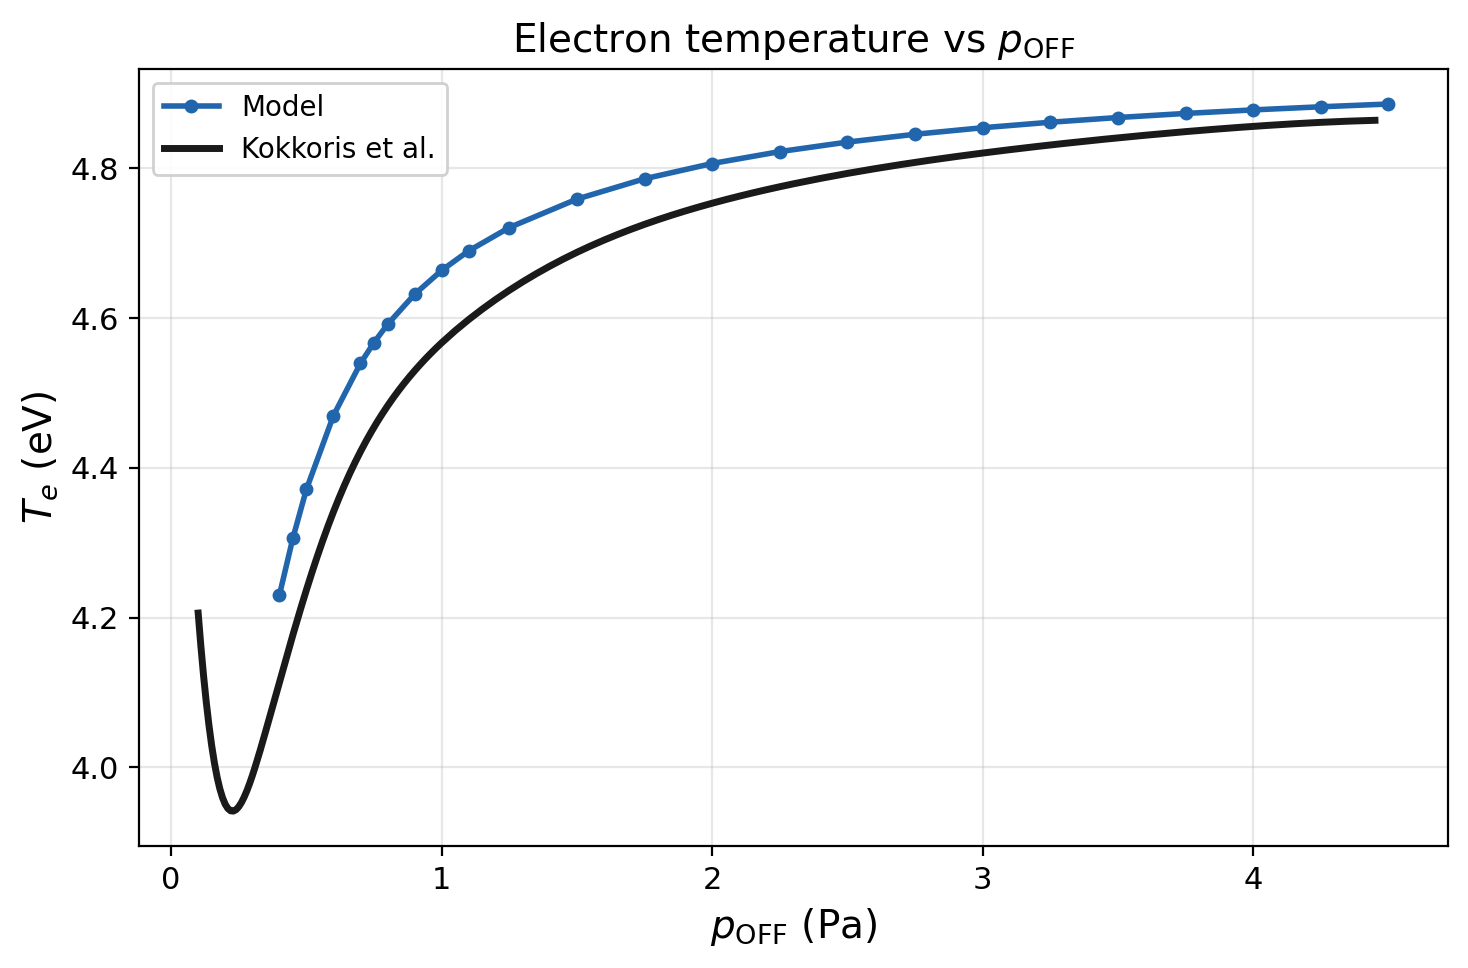
\includegraphics[width=\textwidth]{Te_vs_poff.png}
\caption{$\Te$: near-perfect agreement above \SI{1}{\pascal}.  Both increase with pressure as SF$_6$ enhances attachment.}
\label{fig:Te_poff}
\end{subfigure}\hfill
\begin{subfigure}[t]{0.48\textwidth}
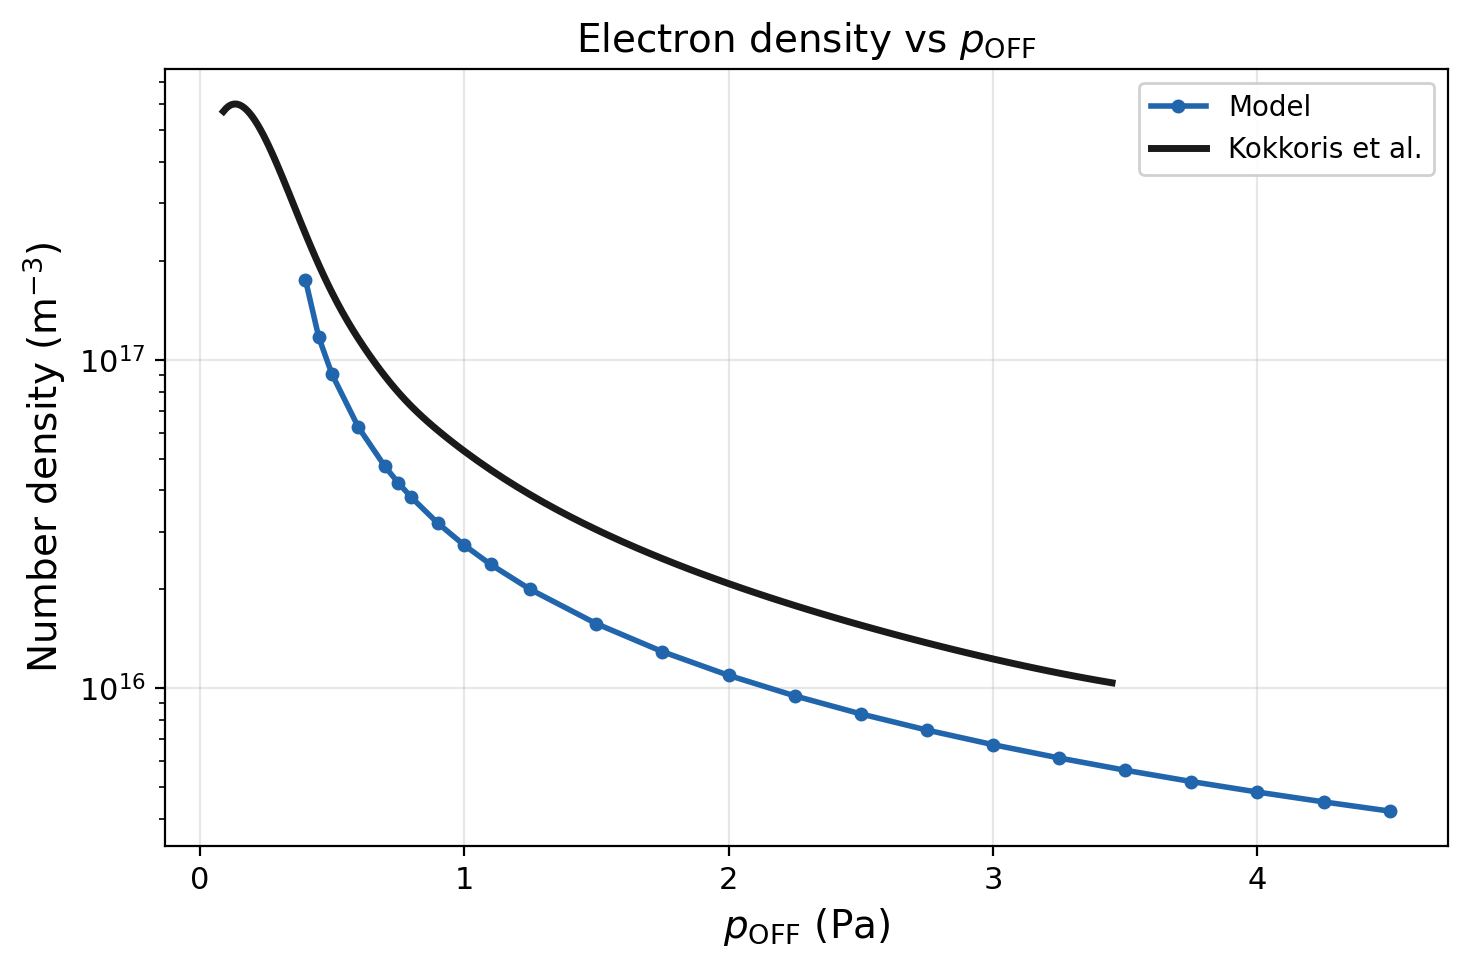
\includegraphics[width=\textwidth]{ne_vs_poff.png}
\caption{$n_e$: ${\sim}2\times$ offset, constant on log scale (multiplicative factor).}
\label{fig:ne_poff}
\end{subfigure}
\caption{$\Te$ and $n_e$ vs $p_\text{OFF}$.}
\label{fig:Te_ne_poff}
\end{figure}

\begin{figure}[H]
\centering
\begin{subfigure}[t]{0.48\textwidth}
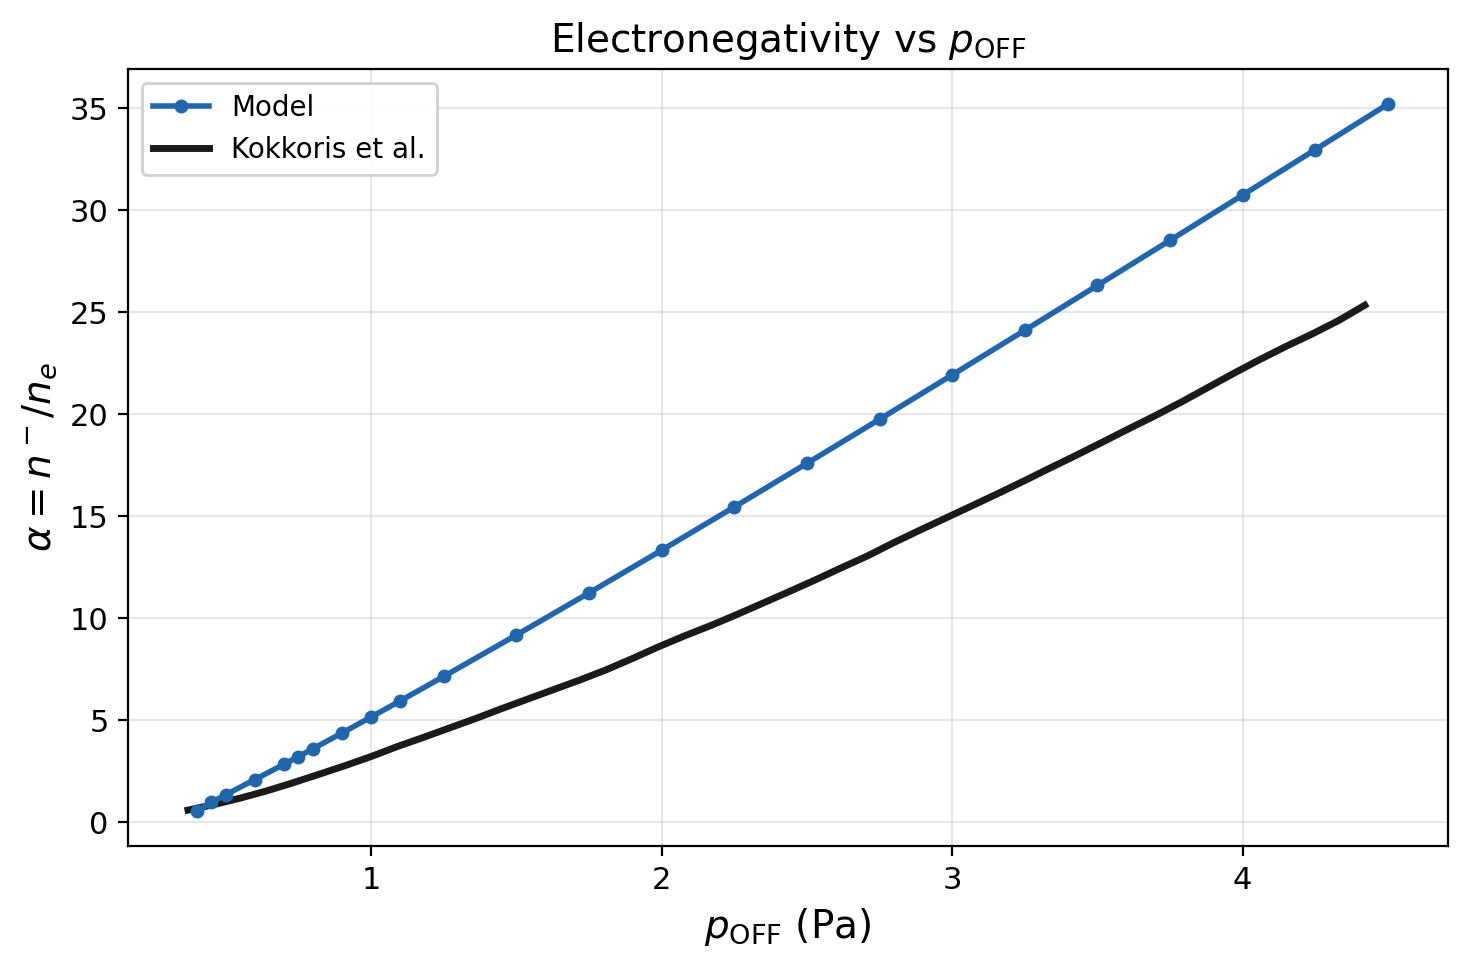
\includegraphics[width=\textwidth]{alpha_vs_poff.png}
\caption{$\alpha$: both increase with pressure.  Model is ${\sim}1.6\times$ higher.}
\label{fig:alpha_poff}
\end{subfigure}\hfill
\begin{subfigure}[t]{0.48\textwidth}
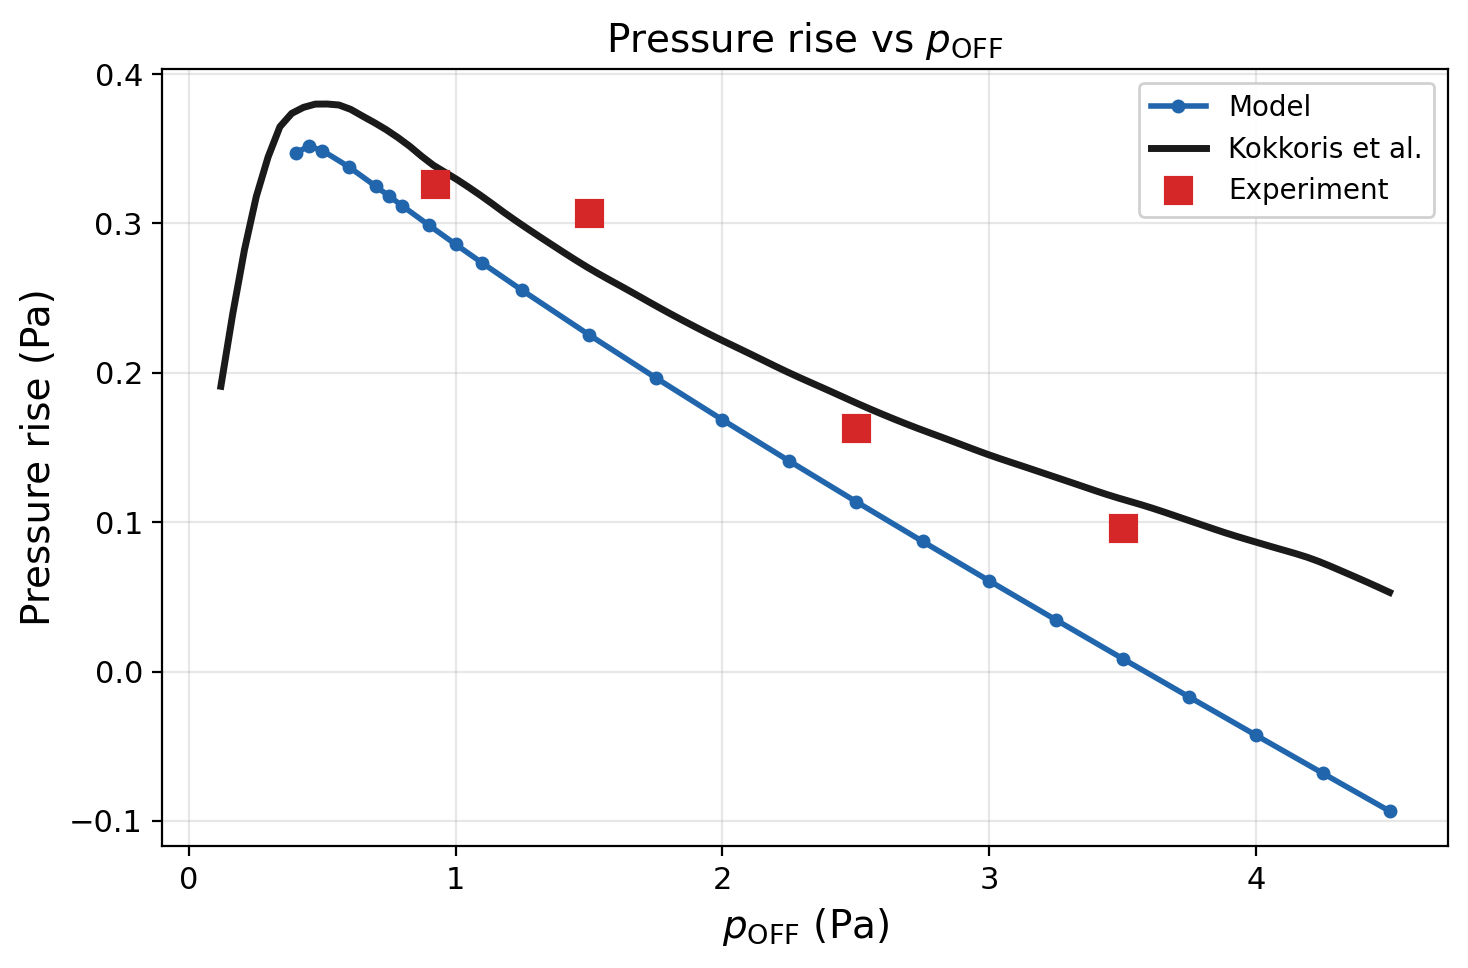
\includegraphics[width=\textwidth]{dp_vs_poff.png}
\caption{Pressure rise: model declines from \SI{0.35}{\pascal}, tracking the experimental trend.}
\label{fig:dp_poff}
\end{subfigure}
\caption{$\alpha$ and $\Delta p$ vs $p_\text{OFF}$.}
\label{fig:alpha_dp_poff}
\end{figure}

\subsection{Neutral Species}
\label{sec:pure_poff_neutrals}

\begin{figure}[H]
\centering
\begin{subfigure}[t]{0.48\textwidth}
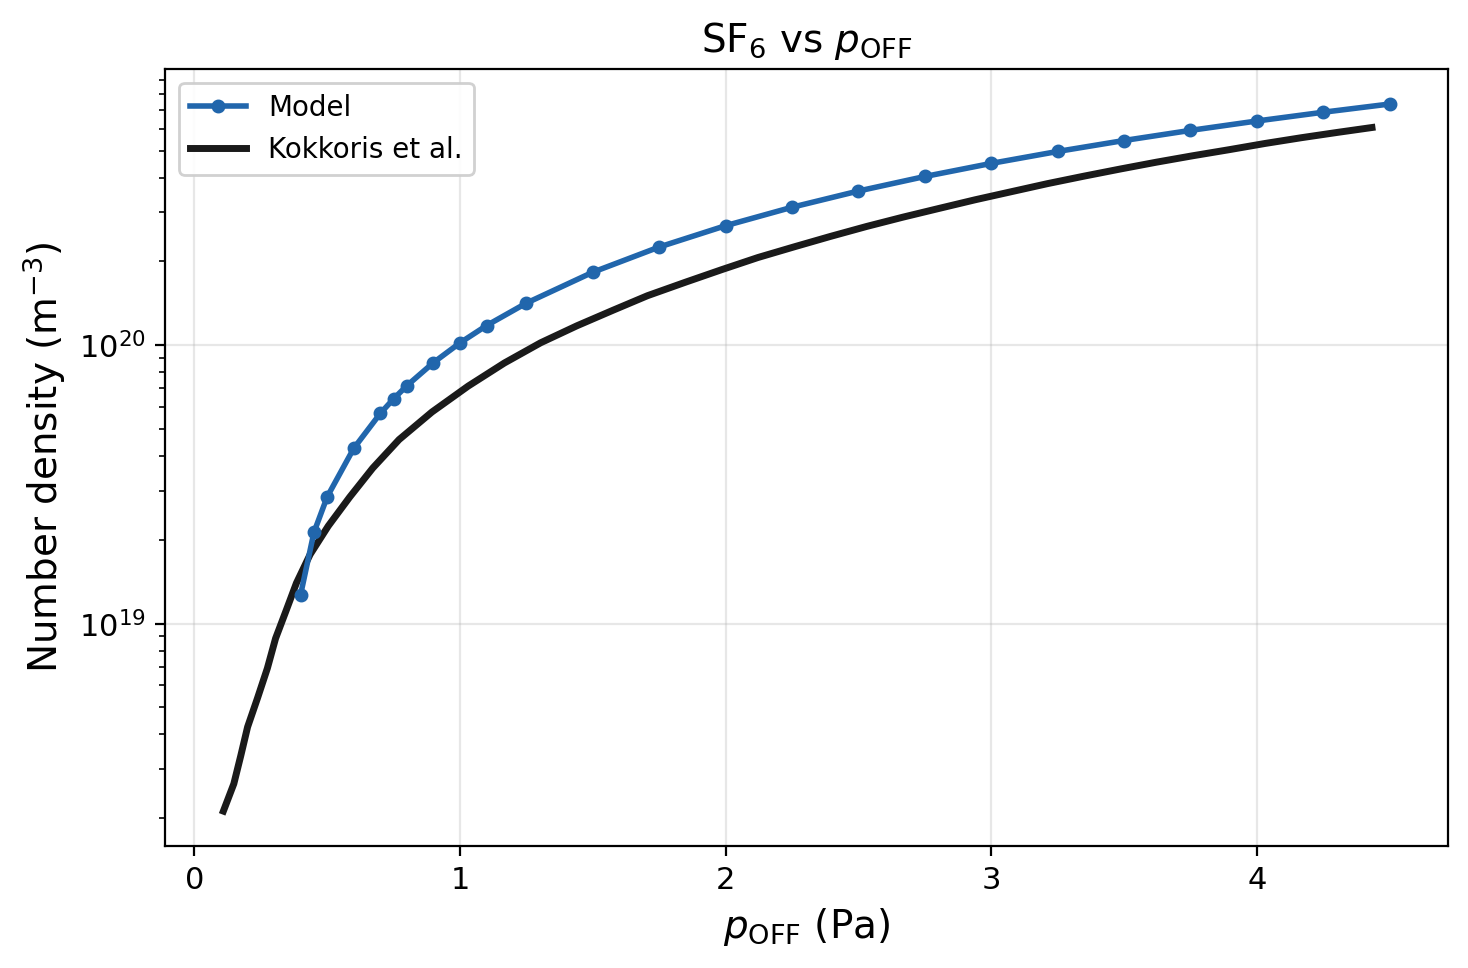
\includegraphics[width=\textwidth]{nSF6_m3_vs_poff.png}
\caption{SF$_6$: both increase steeply.}
\label{fig:nSF6_poff}
\end{subfigure}\hfill
\begin{subfigure}[t]{0.48\textwidth}
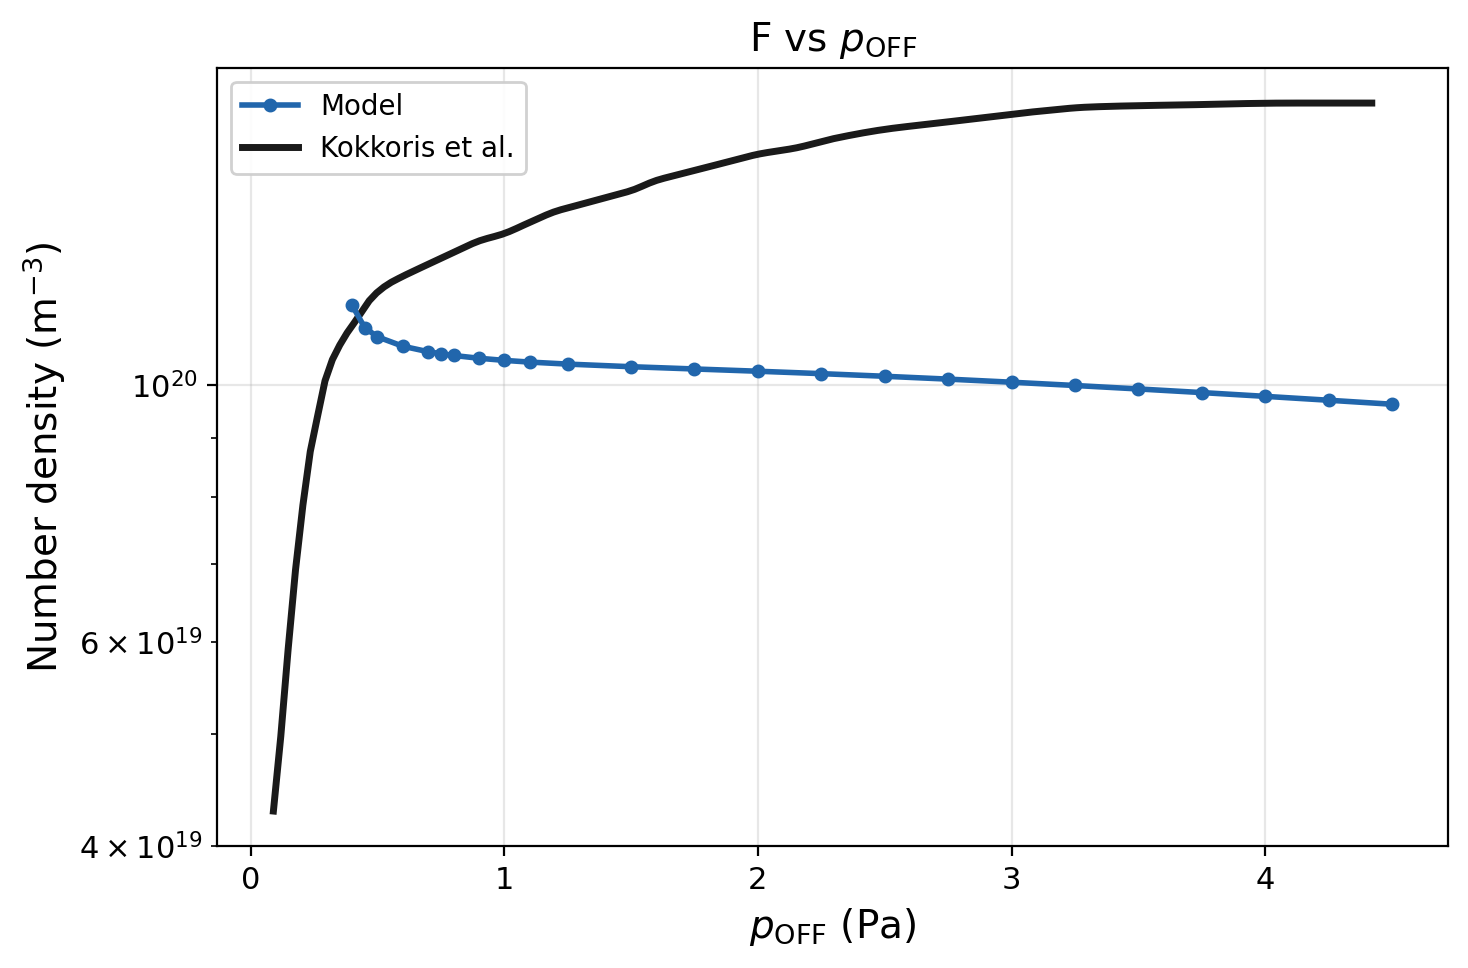
\includegraphics[width=\textwidth]{nF_m3_vs_poff.png}
\caption{F: model rises and plateaus, matching the qualitative trend.}
\label{fig:nF_poff}
\end{subfigure}
\caption{SF$_6$ and F vs $p_\text{OFF}$.}
\label{fig:SF6_F_poff}
\end{figure}

\begin{figure}[H]
\centering
\begin{subfigure}[t]{0.48\textwidth}
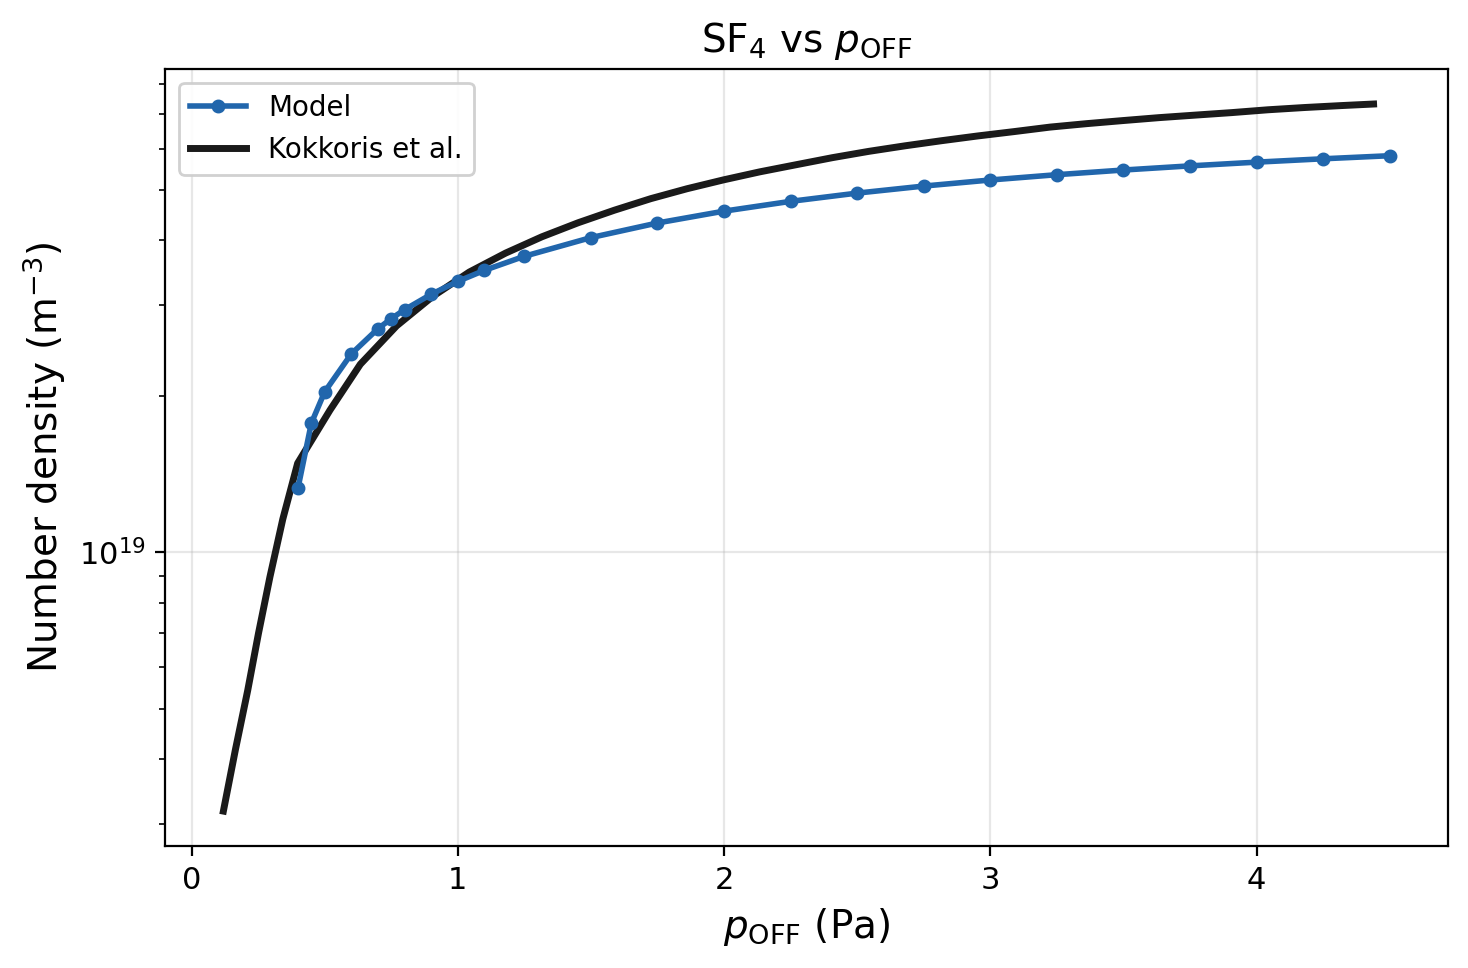
\includegraphics[width=\textwidth]{nSF4_m3_vs_poff.png}
\caption{SF$_4$.}
\label{fig:nSF4_poff}
\end{subfigure}\hfill
\begin{subfigure}[t]{0.48\textwidth}
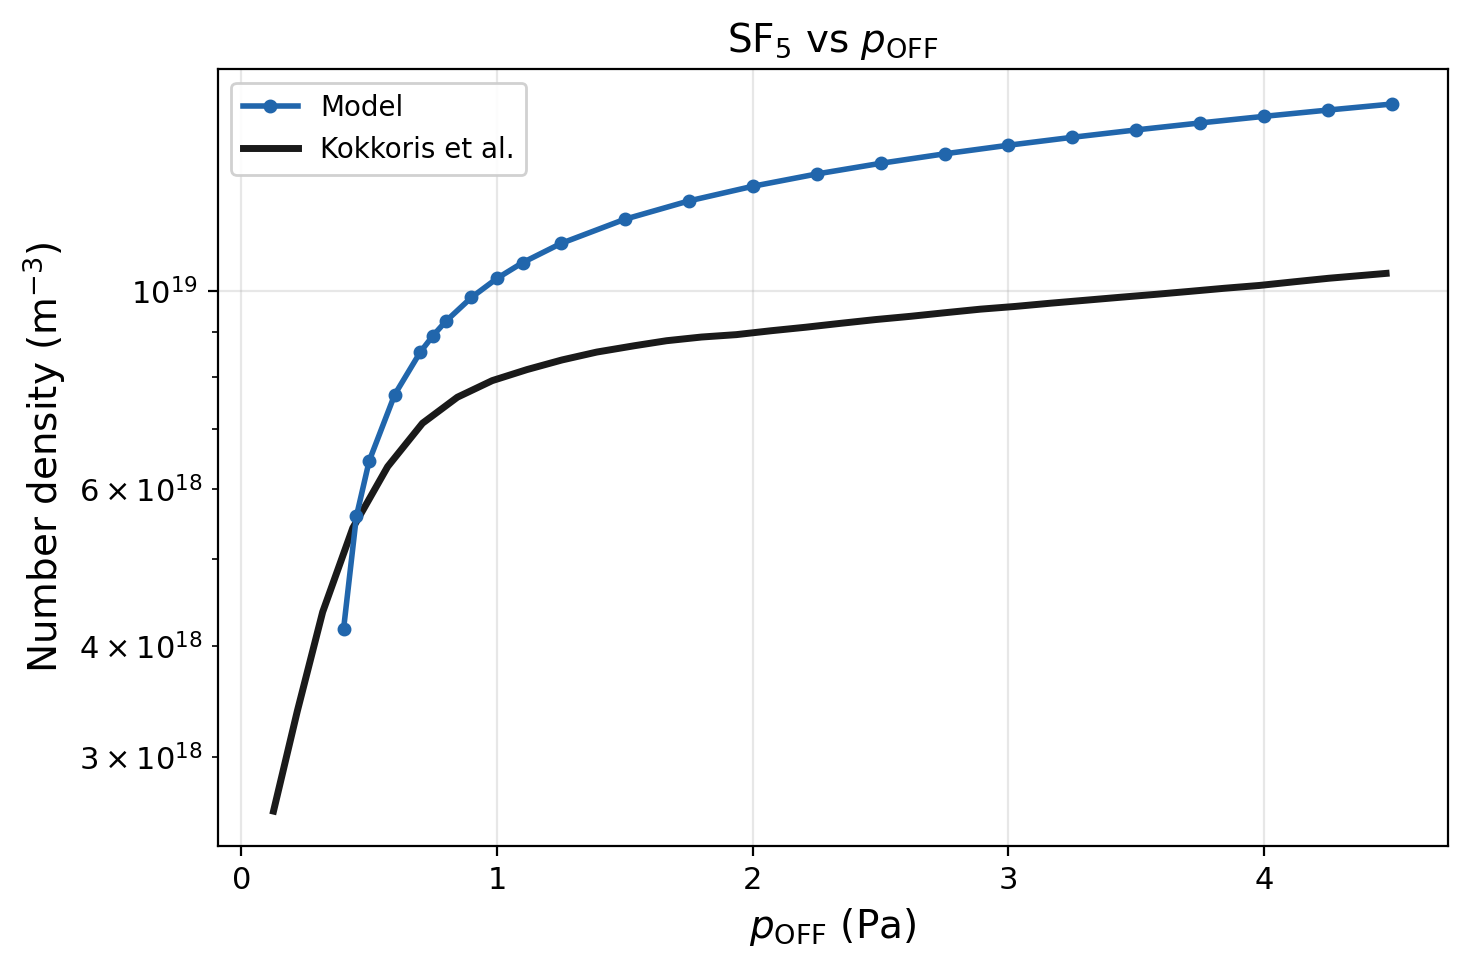
\includegraphics[width=\textwidth]{nSF5_m3_vs_poff.png}
\caption{SF$_5$.}
\label{fig:nSF5_poff}
\end{subfigure}
\caption{SF$_4$ and SF$_5$ vs $p_\text{OFF}$.}
\label{fig:SF4_SF5_poff}
\end{figure}

\begin{figure}[H]
\centering
\begin{subfigure}[t]{0.48\textwidth}
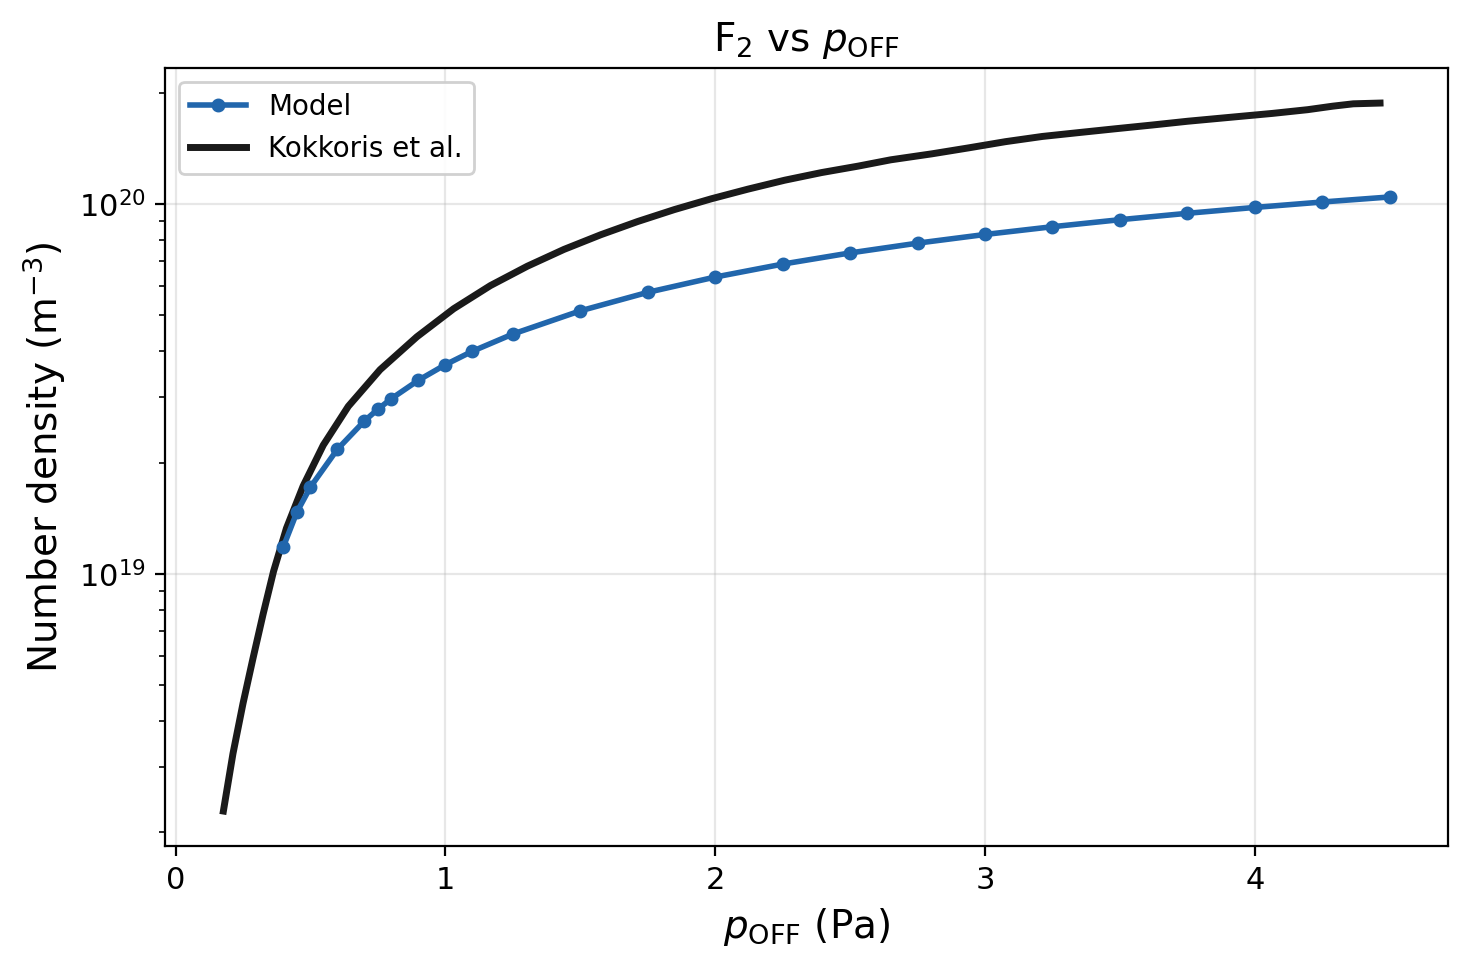
\includegraphics[width=\textwidth]{nF2_m3_vs_poff.png}
\caption{F$_2$.}
\label{fig:nF2_poff}
\end{subfigure}\hfill
\begin{subfigure}[t]{0.48\textwidth}
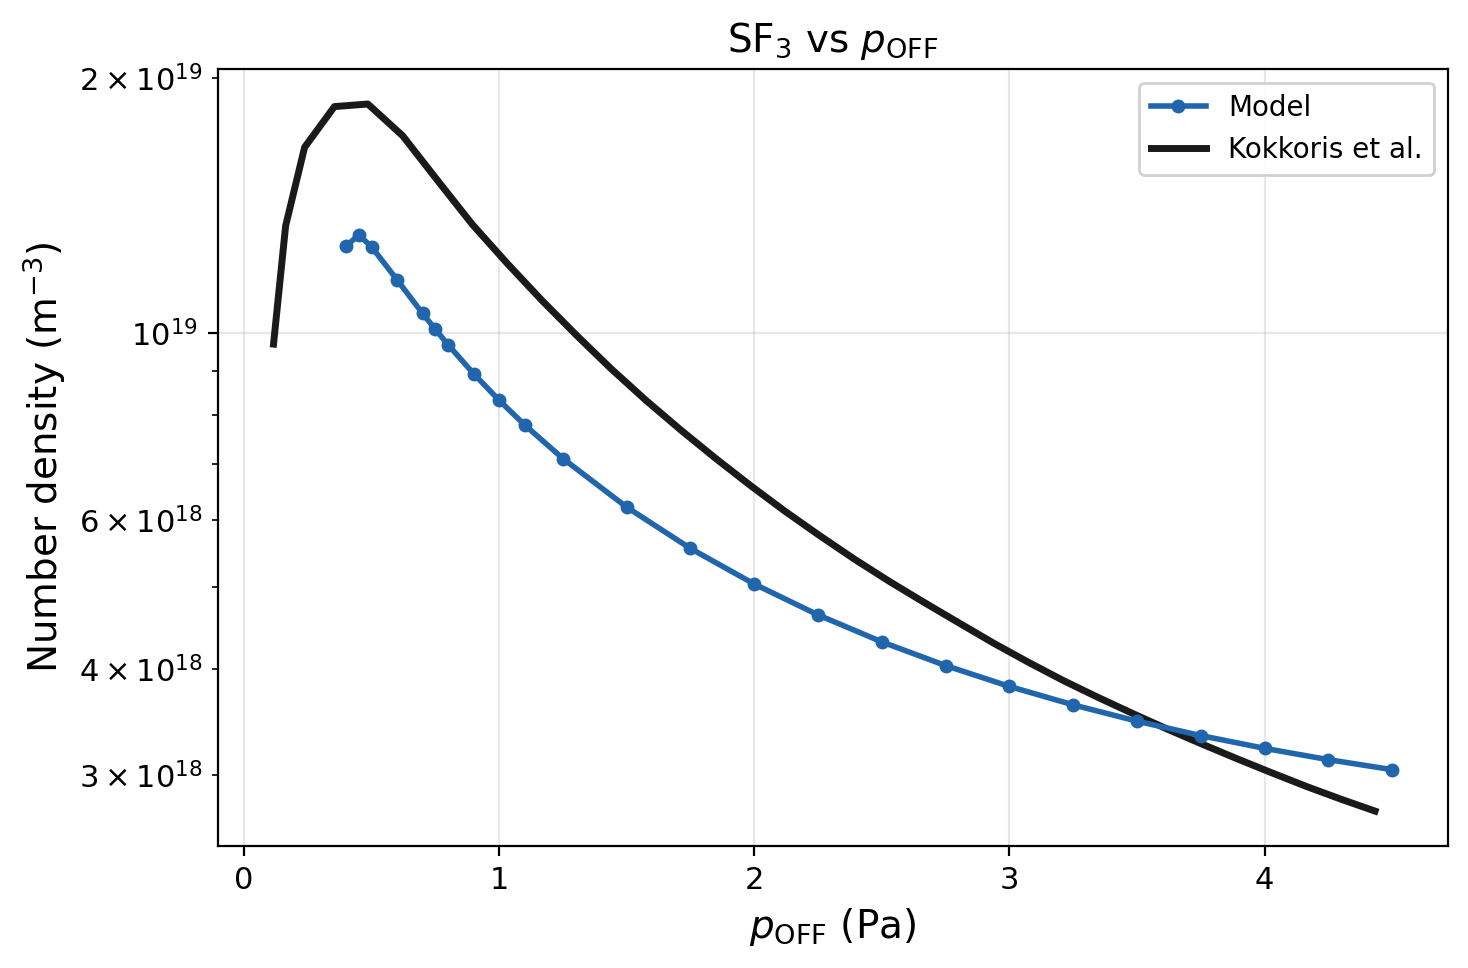
\includegraphics[width=\textwidth]{nSF3_m3_vs_poff.png}
\caption{SF$_3$.}
\label{fig:nSF3_poff}
\end{subfigure}
\caption{F$_2$ and SF$_3$ vs $p_\text{OFF}$.}
\label{fig:F2_SF3_poff}
\end{figure}

\subsection{Charged Species}
\label{sec:pure_poff_charged}

\begin{figure}[H]
\centering
\begin{subfigure}[t]{0.48\textwidth}
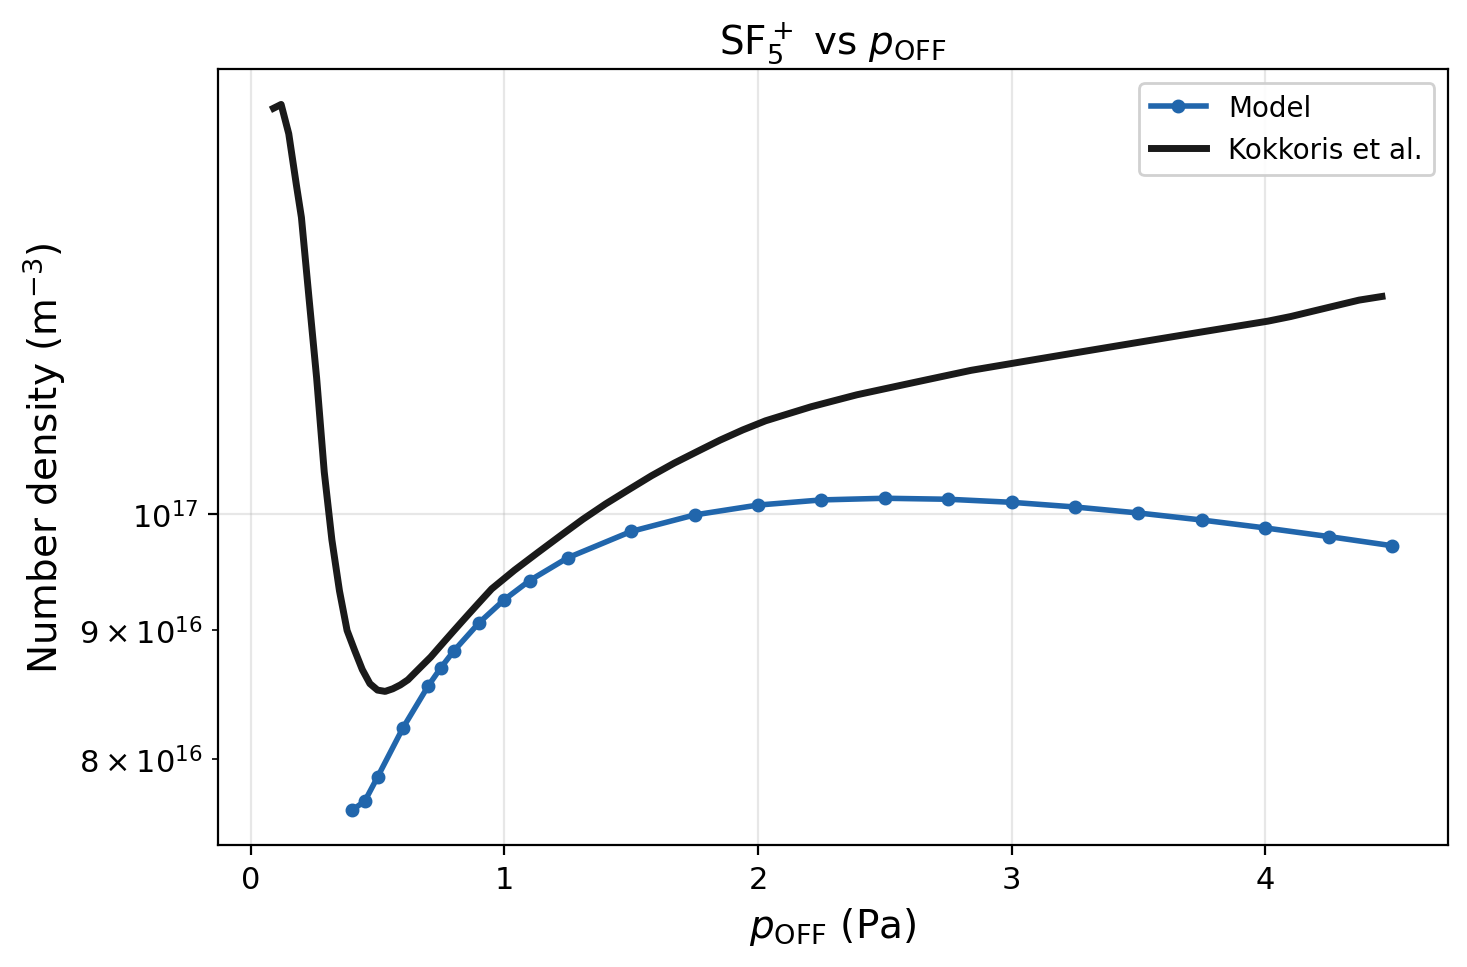
\includegraphics[width=\textwidth]{nSF5p_m3_vs_poff.png}
\caption{SF$_5^+$: dominant positive ion.  Model shows peak at low pressure.}
\label{fig:nSF5p_poff}
\end{subfigure}\hfill
\begin{subfigure}[t]{0.48\textwidth}
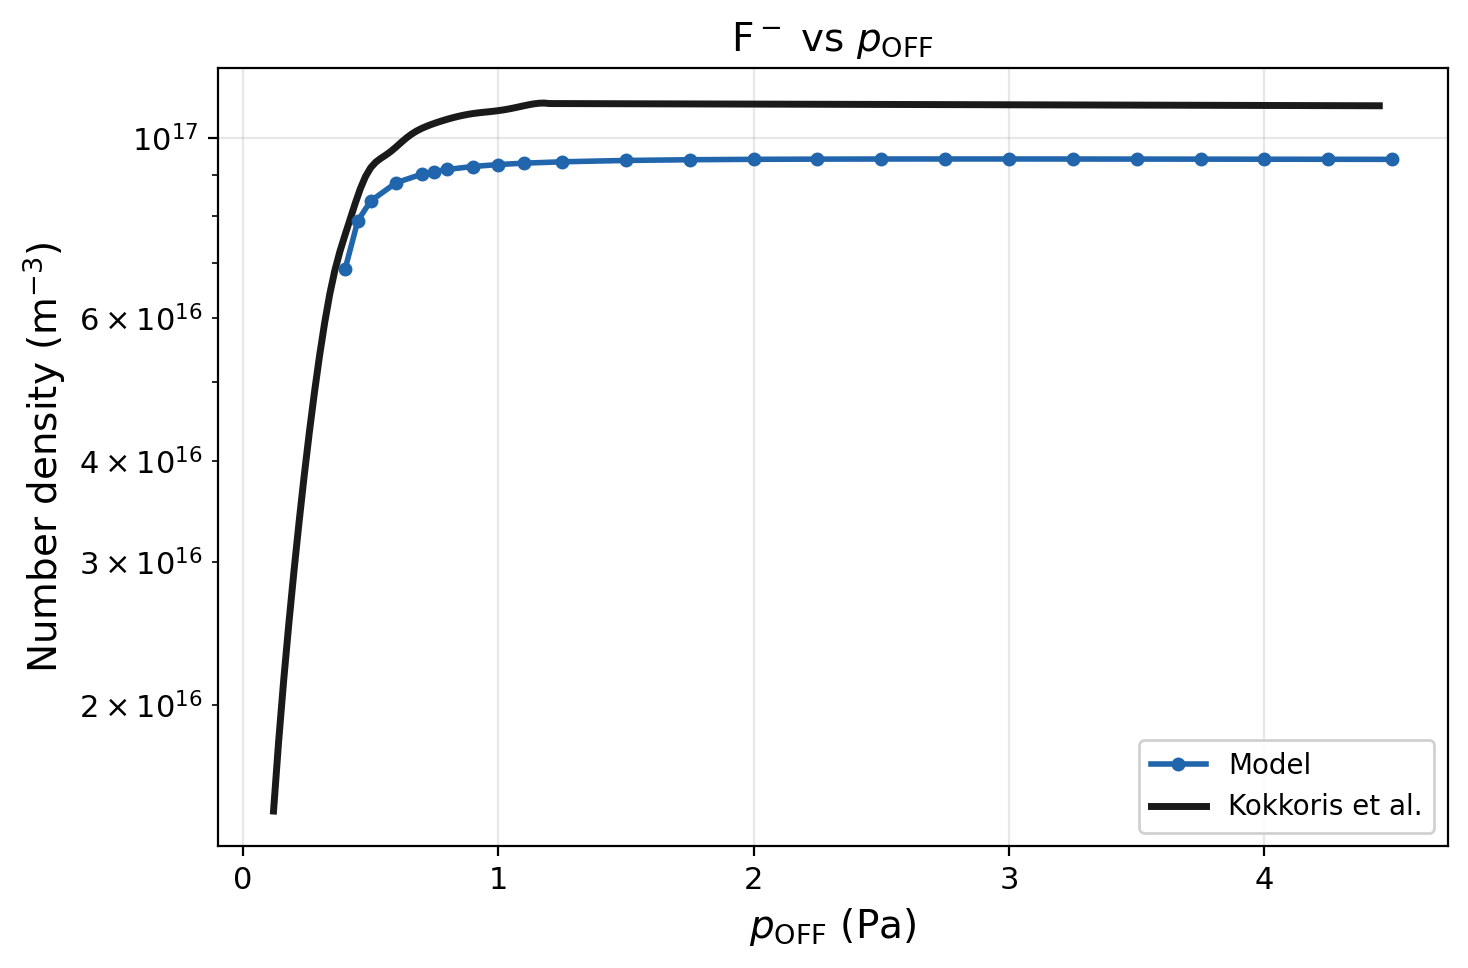
\includegraphics[width=\textwidth]{nFm_m3_vs_poff.png}
\caption{F$^-$: dominant negative ion.}
\label{fig:nFm_poff}
\end{subfigure}
\caption{Dominant ions vs $p_\text{OFF}$.}
\label{fig:dom_ions_poff}
\end{figure}

\begin{figure}[H]
\centering
\begin{subfigure}[t]{0.48\textwidth}
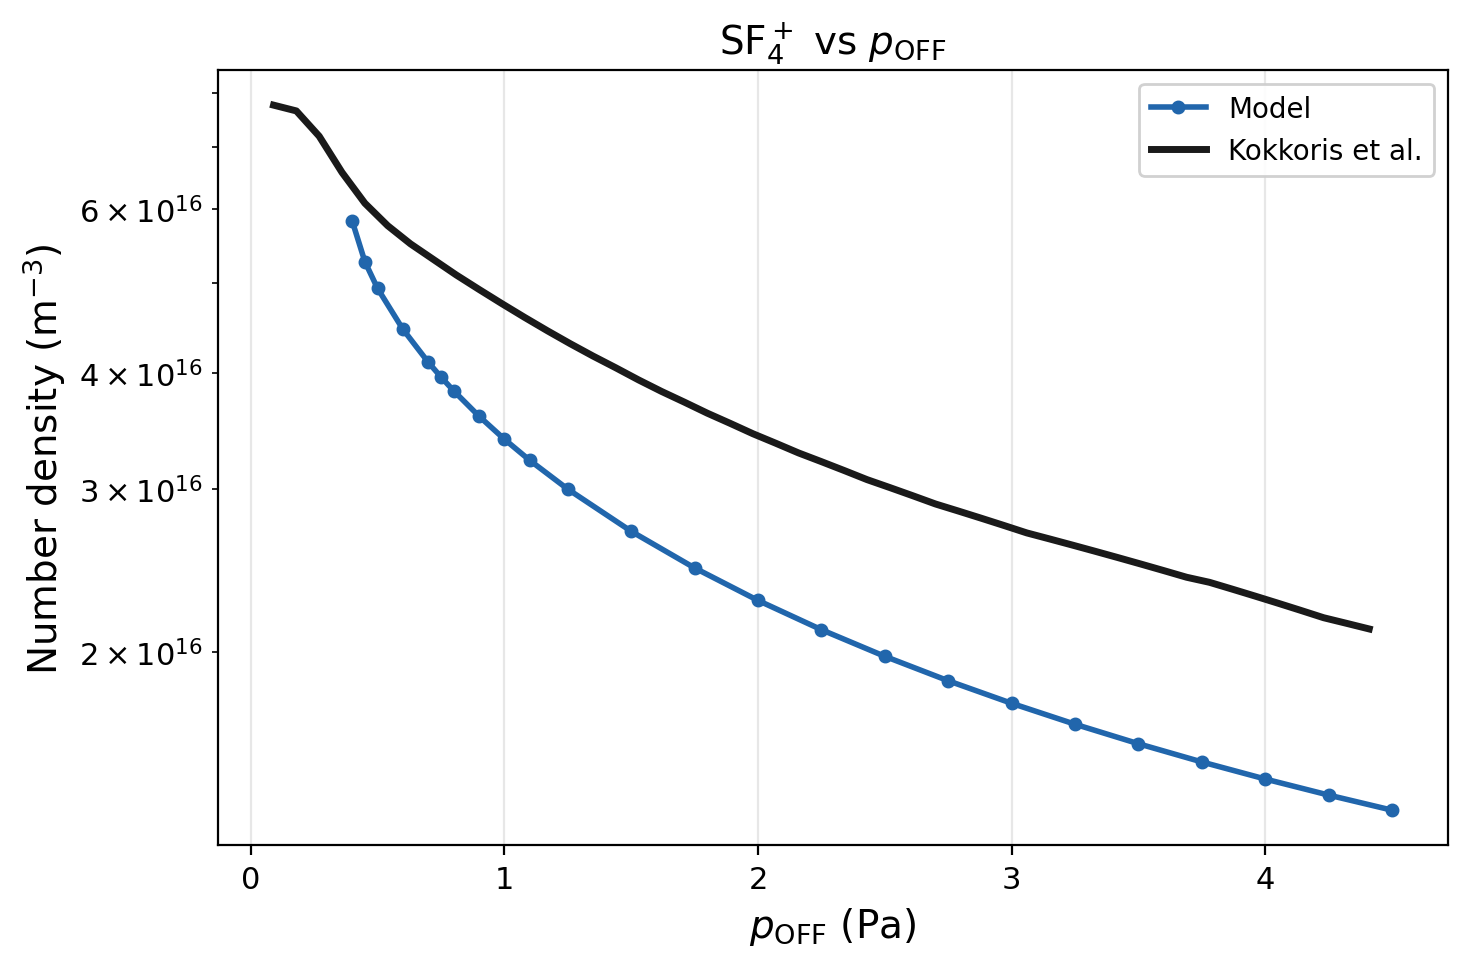
\includegraphics[width=\textwidth]{nSF4p_m3_vs_poff.png}
\caption{SF$_4^+$.}
\label{fig:nSF4p_poff}
\end{subfigure}\hfill
\begin{subfigure}[t]{0.48\textwidth}
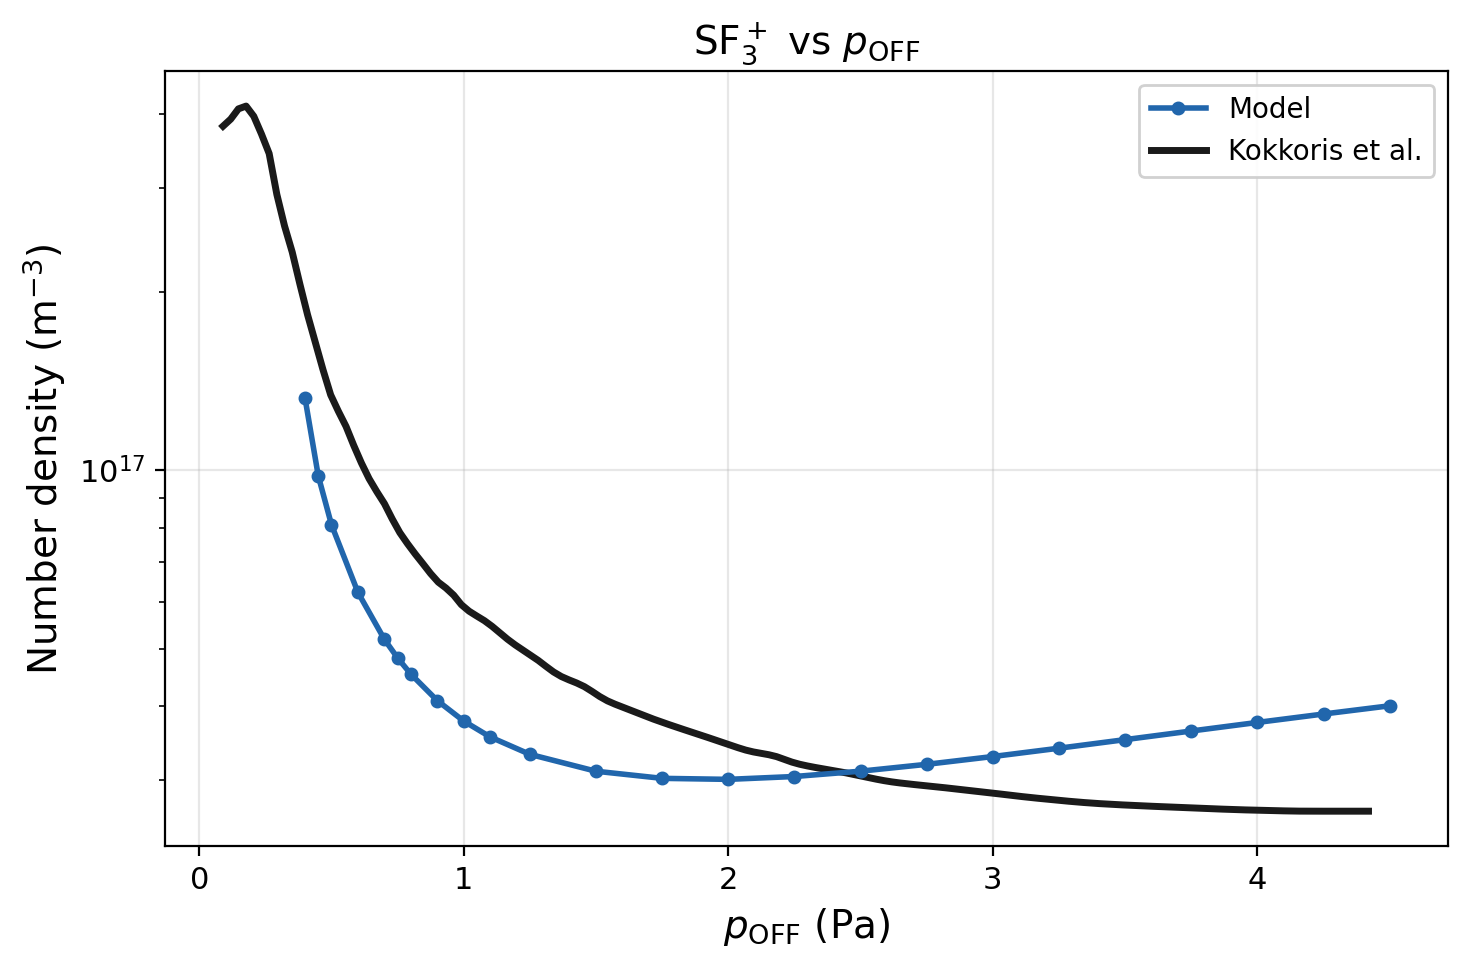
\includegraphics[width=\textwidth]{nSF3p_m3_vs_poff.png}
\caption{SF$_3^+$.}
\label{fig:nSF3p_poff}
\end{subfigure}
\caption{Secondary ions vs $p_\text{OFF}$.}
\label{fig:sec_ions_poff}
\end{figure}

\begin{figure}[H]
\centering
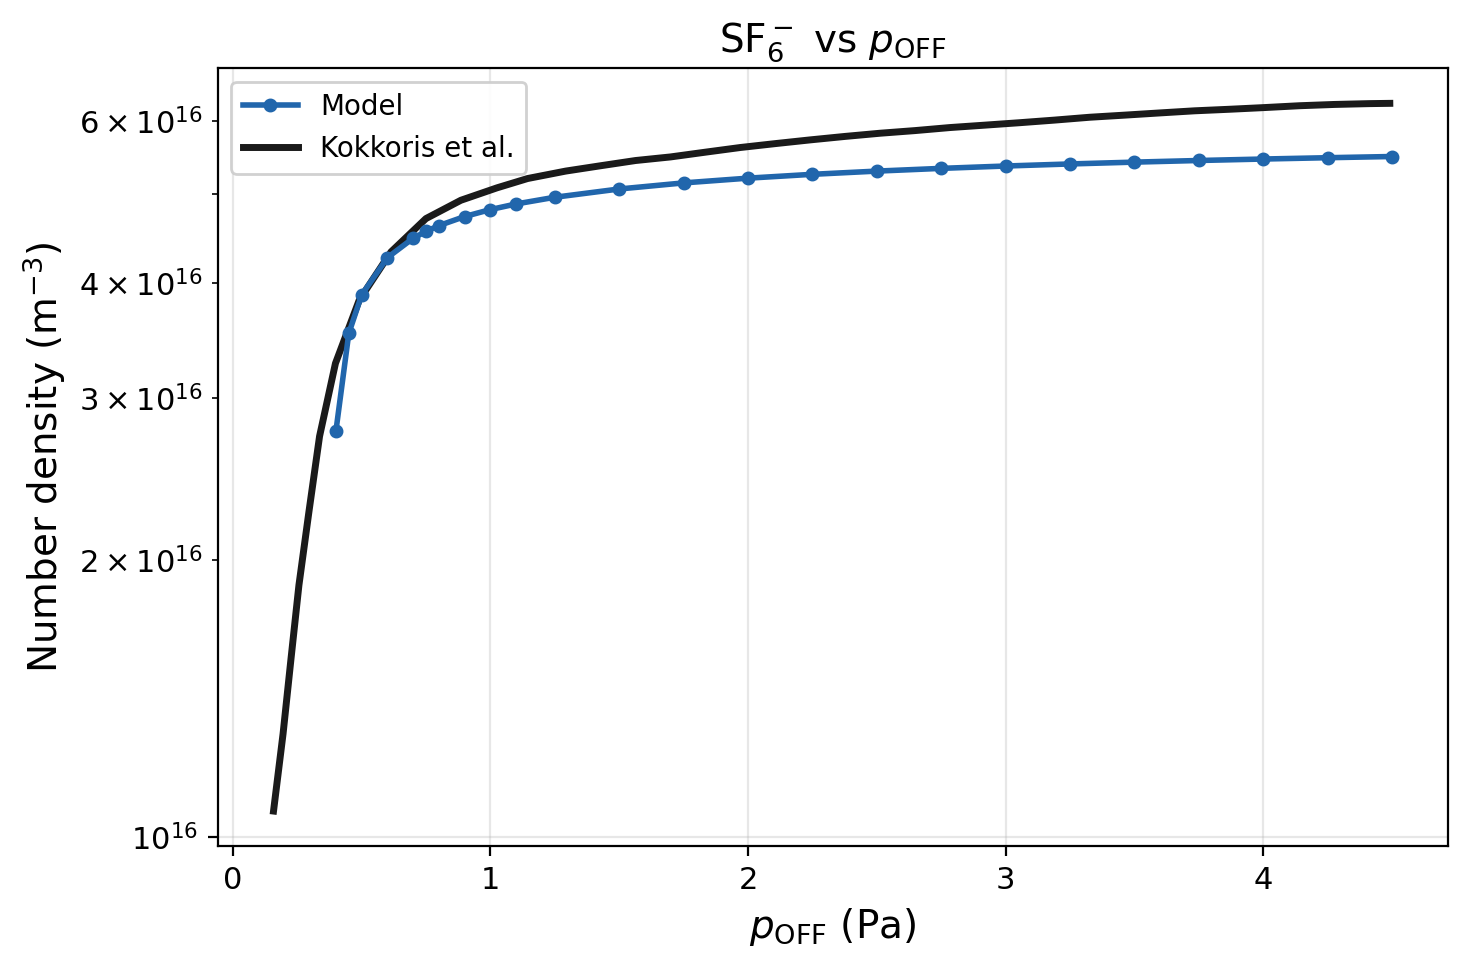
\includegraphics[width=0.55\textwidth]{nSF6m_m3_vs_poff.png}
\caption{SF$_6^-$ vs $p_\text{OFF}$.}
\label{fig:nSF6m_poff}
\end{figure}

\subsection{F Density with Experimental Data}
\label{sec:pure_poff_Fexp}

\begin{figure}[H]
\centering
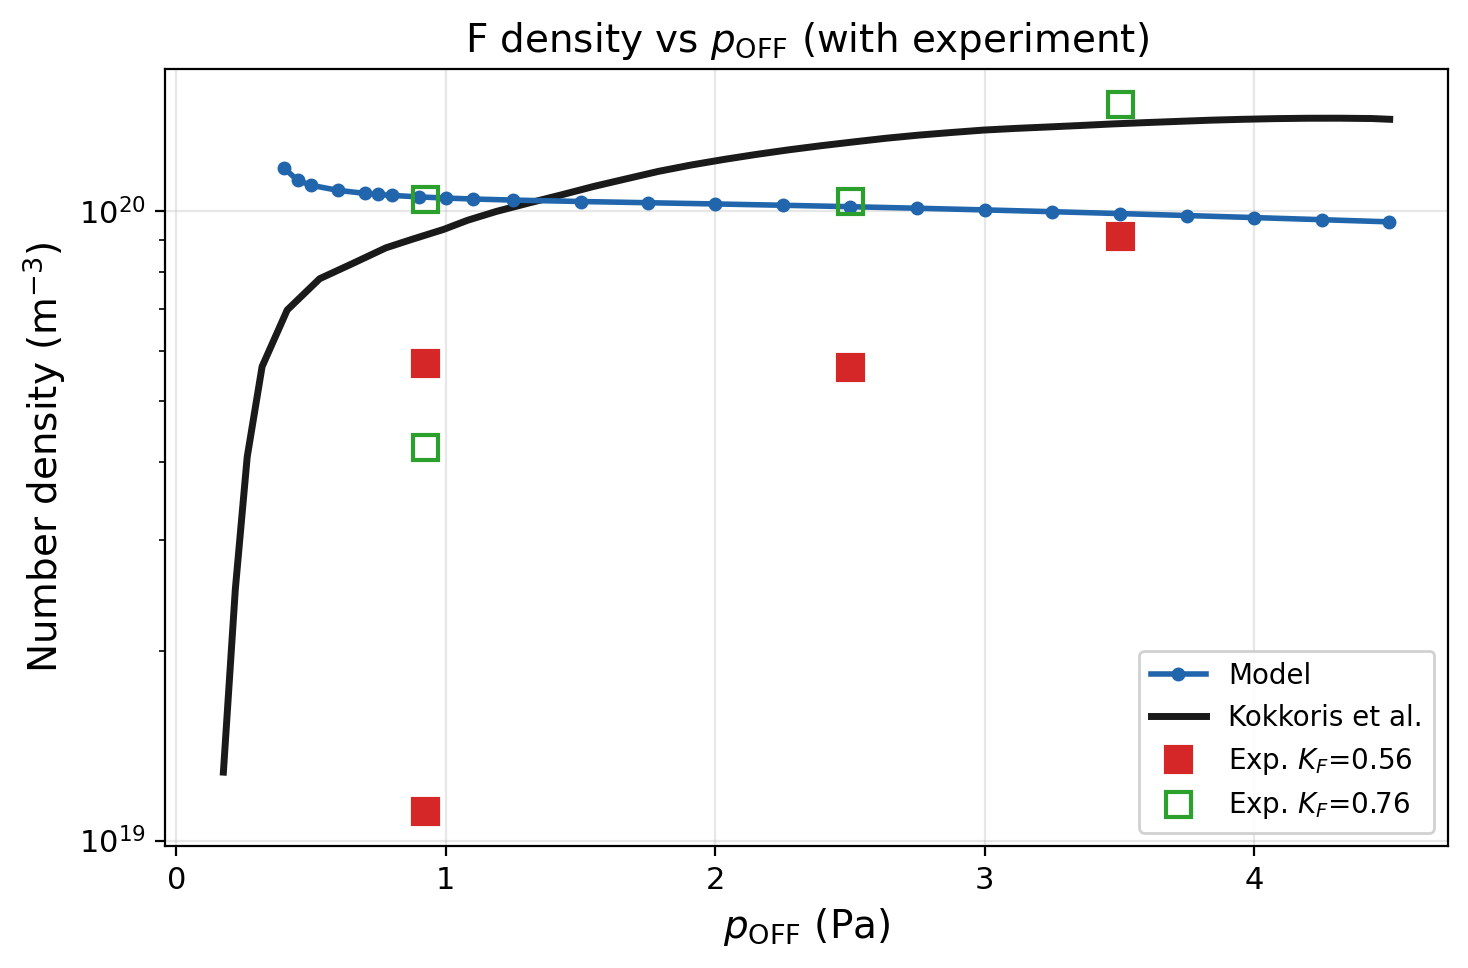
\includegraphics[width=0.65\textwidth]{nF_with_exp_vs_poff.png}
\caption{F density vs $p_\text{OFF}$ with experimental actinometry data.}
\label{fig:nF_exp_poff}
\end{figure}

%======================================================================
\section{Quantitative Comparison}
\label{sec:pure_quantitative}
%======================================================================

\begin{table}[H]
\centering
\caption{Model vs Kokkoris et al.~\cite{Kokkoris2009} at \SI{2000}{\watt}, $p_\text{OFF} = \SI{0.921}{\pascal}$.}
\label{tab:pure_comparison}
\begin{tabular}{lccl}
\toprule
\textbf{Quantity} & \textbf{Model} & \textbf{Ratio} & \textbf{Assessment} \\
\midrule
$\Te$ (eV) & 4.64 & 1.02$\times$ & Excellent \\
SF$_4$ & $3.2\times10^{19}$ & 1.01$\times$ & Excellent \\
SF$_6^-$ & $4.7\times10^{16}$ & 0.94$\times$ & Excellent \\
SF$_5^+$ & $9.1\times10^{16}$ & 0.91$\times$ & Good \\
F & $1.1\times10^{20}$ & 0.81$\times$ & Good \\
F$^-$ & $9.2\times10^{16}$ & 0.78$\times$ & Good \\
F$_2$ & $3.4\times10^{19}$ & 0.76$\times$ & Good \\
SF$_3$ & $8.9\times10^{18}$ & 0.68$\times$ & Good \\
$\alpha$ & 4.5 & 1.64$\times$ & Fair \\
SF$_6$ & $8.8\times10^{19}$ & 1.47$\times$ & Fair \\
SF$_5$ & $9.9\times10^{18}$ & 1.26$\times$ & Good \\
$n_e$ (m$^{-3}$) & $3.1\times10^{16}$ & \textbf{0.49$\times$} & \textbf{See below} \\
\bottomrule
\end{tabular}
\end{table}

%======================================================================
\section{Discrepancy Analysis}
\label{sec:pure_discrepancy}
%======================================================================

\subsection{Electron Density Offset}
\label{sec:pure_ne_offset}

The model predicts an electron density approximately $2\times$ lower than the reference across both the power and pressure sweeps.  This manifests as a constant multiplicative offset on the logarithmic scale, consistent with a systematic origin rather than a species-specific error.  The downstream discrepancies---SF$_6$ density too high, F density too low, and $\alpha$ too high---can all be traced to this single root cause.

\subsection{Root Cause Decomposition}
\label{sec:pure_rootcause}

The offset decomposes into two multiplicative factors:

\textbf{Power coupling (${\sim}1.3\times$).}  The model uses $\eta = 0.70$; the reference assumes $P_\text{abs} = P_\text{source}$ ($\eta = 1$).  Since $n_e \propto \eta^{0.8}$, this accounts for $0.70^{0.8} \approx 0.76$, i.e.\ $1.3\times$ reduction.

\textbf{Geometry and solver (${\sim}1.5\times$).}  The present model represents the reactor as a single equivalent cylinder with radius $R = \SI{0.19}{\meter}$ and length $L = \SI{0.38}{\meter}$.  In practice, the GIR~300 reactor used in Kokkoris et al.~\cite{Kokkoris2009} has a multi-region structure consisting of an ICP source region and a separate processing region, connected by a narrow aperture.  This two-chamber geometry affects the discharge in several ways: (i)~the effective diffusion length $\Lambda$ is shorter in each sub-chamber, increasing ion wall loss rates; (ii)~the spatial distribution of power deposition is non-uniform; (iii)~species transport between the two regions introduces additional loss channels not captured by the single-zone approximation.

\subsection{Residual Offset Assessment}
\label{sec:pure_residual}

At the operating electronegativity ($\alpha = 3$--5), modern $h$-factor formulations (Kim, Thorsteinsson, Monahan) agree to within 10\%, and the $h$-factor choice contributes only a ${\sim}5\%$ improvement in $n_e$.  The offset is therefore documented as a calibration-level discrepancy inherent to the independent reconstruction of a global model from published data alone.

%======================================================================
\section{Summary}
\label{sec:pure_summary}
%======================================================================

A zero-dimensional global model for SF$_6$ ICP discharges has been independently reconstructed from the published reaction set of Kokkoris et al.~\cite{Kokkoris2009} and validated against both simulation and experimental data.  The electron temperature is reproduced within 2\%, and 10 of 12 species densities agree within a factor of~2.  All qualitative trends---including the dissociation cascade, electronegativity evolution, and pressure rise behaviour---are correctly captured in both power and pressure sweeps.

The residual ${\sim}2\times$ electron density offset is attributed to the power coupling efficiency and the single-cylinder geometry approximation.  Closing this gap would require either independent characterisation of the power transfer efficiency or spatially resolved modelling of the multi-chamber reactor geometry, both of which fall outside the scope of a zero-dimensional reconstruction.

The validated pure $\SFsix$ model provides the foundation for extending to $\SFsix/\Ar$ mixtures in the next chapter, where argon dilution introduces new ionization pathways (direct, stepwise, and Penning), metastable dynamics, and a composition-dependent electronegative-to-electropositive transition.


%=============================================================================
\chapter{SF\texorpdfstring{$_6$}{6}/Ar Gas-Phase Model}
\label{ch:sf6ar_gasphase}
%=============================================================================

This chapter documents the reproduction of the Lallement et al.~\cite{Lallement2009} comprehensive zero-dimensional model for $\SFsix/\Ar$ plasmas in an ICP reactor.  The model extends the pure $\SFsix$ chemistry of Chapter~\ref{ch:pure_sf6} to include 26 species, 54 gas-phase reactions, Maxwellian EEDF rate coefficients, and detailed treatment of argon metastable dynamics including Penning ionization and quenching by molecular species.

%======================================================================
\section{Physical Model}
\label{sec:gasphase_model}
%======================================================================

\subsection{Reactor Geometry and Assumptions}
\label{sec:gasphase_geometry}

The model assumes a cylindrical ICP reactor with radius $R = \SI{0.180}{\meter}$ and height $L = \SI{0.175}{\meter}$.  The plasma is treated as a spatially uniform (zero-dimensional) volume-averaged system at steady state.  The gas temperature is fixed at $T_\mathrm{gas} = \SI{300}{\kelvin}$, and the negative ion temperature is $T_- = \SI{0.3}{\electronvolt}$.  The gas flow rate is $Q = \SI{40}{sccm}$ of $\SFsix/\Ar$ mixture, defining a residence time
\begin{equation}
\tau_R = \frac{p V}{Q_{T,P}}
\label{eq:gas_tau}
\end{equation}
where $p$ is the operating pressure and $Q_{T,P}$ is the volumetric flow rate converted to operating conditions.

\subsection{Species}
\label{sec:gasphase_species}

The model tracks 26 species in total.

\paragraph{Neutrals (9):} $\SFsix$, $\SFfive$, $\SFfour$, $\SFthree$, SF$_2$, SF, S, F, F$_2$.

\paragraph{Positive ions (7):} SF$_5^+$, SF$_4^+$, SF$_3^+$, SF$_2^+$, SF$^+$, S$^+$, F$^+$, plus Ar$^+$.

\paragraph{Negative ions (7):} SF$_6^-$, SF$_5^-$, SF$_4^-$, SF$_3^-$, SF$_2^-$, F$^-$, F$_2^-$.

\paragraph{Argon species:} Ar (ground state), Ar$^+$ (ion), Ar$^*$ (${}^3P_2$ metastable).

\subsection{Gas-Phase Reaction Set}
\label{sec:gasphase_rxnset}

The full reaction set comprises 54 electron-impact and heavy-particle reactions, organized into the following categories:

\begin{enumerate}[label=(\roman*)]
\item \textbf{SF$_6$ dissociation} (5 channels): Single-step dissociation of $\SFsix$ into $\SFfive + \mathrm{F}$, $\SFfour + 2\mathrm{F}$, $\SFthree + 3\mathrm{F}$, plus multi-step paths producing F$_2$.
\item \textbf{Sequential SFx dissociation} (5 reactions): $\SFfive \to \SFfour + \mathrm{F}$, down to $\mathrm{SF} \to \mathrm{S} + \mathrm{F}$.
\item \textbf{Dissociative ionization of SF$_6$} (7 channels): Producing SF$_5^+$ through F$^+$.
\item \textbf{Ionization of fragments}: SF$_5$, SF$_3$, F, S.
\item \textbf{Dissociative attachment} (7 channels): $\SFsix + e \to \SFfive^- + \mathrm{F}$, etc.
\item \textbf{Neutral recombination} (9 reactions): $\SFx + \mathrm{F} \to \SFx[x+1]$ and disproportionation.
\item \textbf{Ion--ion recombination}: All positive--negative ion pairs.
\item \textbf{Argon reactions}: Direct ionization, excitation (to Ar$^*$), stepwise ionization from Ar$^*$, superelastic quenching, elastic scattering, and metastable--metastable ionization.
\end{enumerate}

Rate coefficients for electron-impact reactions take the Arrhenius-like form
\begin{equation}
k = A \exp\!\left(-\frac{E_\mathrm{th}}{\Te}\right) \quad [\text{cm}^3\,\text{s}^{-1}]
\label{eq:gas_arrhenius}
\end{equation}
where $\Te$ is the electron temperature in eV and $E_\mathrm{th}$ is the threshold energy.

%======================================================================
\section{Governing Equations}
\label{sec:gasphase_gov}
%======================================================================

\subsection{Neutral Species Mass Balance}
\label{sec:gasphase_neutral}

For each neutral species $j$, the steady-state mass balance equates the production rate (feed inflow plus gas-phase and surface production) to the destruction rate (electron-impact consumption, wall loss, and pumping).  The feed term acts only on the parent gas species ($\SFsix$ and Ar), while the wall loss term depends on the species-specific diffusion coefficient and wall reaction probability.  This balance determines the steady-state density of each neutral in terms of the electron density and temperature:
\begin{equation}
\boxed{\frac{n_{j,\mathrm{feed}}}{\tau_R} + \sum_r \nu_{jr}^+ R_r = n_j \left( \sum_r \nu_{jr}^- k_r n_e + k_{w,j} + \frac{1}{\tau_R} \right)}
\label{eq:gas_neutral_balance}
\end{equation}
where $\nu_{jr}^\pm$ are stoichiometric production/consumption coefficients, $R_r$ are volumetric reaction rates, and $k_{w,j}$ is the wall loss rate for species $j$.

\subsection{Charged Particle Balances}
\label{sec:gasphase_charged}

\paragraph{Positive ions.} The total positive ion density $n_+$ is governed by the balance between ionization (the dominant production mechanism), wall loss (for ions that reach the sheath edge), and volume recombination with negative ions.  In strongly electronegative plasmas ($\alpha \gg 1$), the ion--ion recombination term dominates over wall loss because the ambipolar field is weakened by the presence of negative ions:
\begin{equation}
\boxed{R_\mathrm{iz} n_e = k_w^+ n_+ + k_\mathrm{rec} n_+ n_-}
\label{eq:gas_posion}
\end{equation}
where $R_\mathrm{iz}$ is the total ionization rate coefficient, $k_w^+$ is the ion wall loss rate, and $k_\mathrm{rec} = 1.5 \times 10^{-9}$\,cm$^3$\,s$^{-1}$ is the ion--ion recombination rate coefficient.

\paragraph{Negative ions.} Negative ions are produced exclusively by dissociative attachment to $\SFsix$ and destroyed solely by volume recombination with positive ions, since the ambipolar sheath confines them away from the walls:
\begin{equation}
\boxed{R_\mathrm{att} n_e = k_\mathrm{rec} n_+ n_-}
\label{eq:gas_negion}
\end{equation}

\paragraph{Charge neutrality:}
\begin{equation}
n_+ = n_e + n_- = n_e(1 + \alpha)
\label{eq:gas_charge}
\end{equation}
where $\alpha \equiv n_-/n_e$ is the electronegativity parameter.

\subsection{Electronegativity Parameter}
\label{sec:gasphase_alpha}

Combining the negative ion balance \eqref{eq:gas_negion} with charge neutrality yields a quadratic equation for $\alpha$.  This equation captures the fundamental competition between attachment (which increases $\alpha$) and ionization plus wall loss (which decrease it).  The physically meaningful root is always the positive one, since $\alpha$ must be non-negative:
\begin{equation}
\boxed{\alpha(1+\alpha) = \frac{R_\mathrm{att}}{k_\mathrm{rec}\,n_e}}
\label{eq:gas_alpha_quad}
\end{equation}
with the physical root
\begin{equation}
\alpha = \frac{-1 + \sqrt{1 + 4\,R_\mathrm{att}/(k_\mathrm{rec}\,n_e)}}{2}
\label{eq:gas_alpha_root}
\end{equation}

\subsection{Electron Temperature (Particle Balance)}
\label{sec:gasphase_Te}

The electron temperature $\Te$ is not a free parameter but is self-consistently determined by the particle balance: at steady state, the total rate of electron production (ionization plus Penning ionization) must exactly equal the total rate of electron loss (attachment plus ion wall loss).  This balance determines $\Te$ because the ionization and attachment rate coefficients have different $\Te$-dependencies, so there exists a unique $\Te$ at which the balance is satisfied.  Higher $\Te$ favors ionization over attachment, while lower $\Te$ favors attachment:
\begin{equation}
\boxed{R_\mathrm{iz}(\Te) + \frac{R_\mathrm{Penn}}{n_e} = R_\mathrm{att}(\Te) + k_w^+(\Te,\alpha)(1+\alpha)}
\label{eq:gas_Te_balance}
\end{equation}
where $R_\mathrm{Penn}/n_e$ is the Penning ionization contribution.  This equation is solved for $\Te$ using the Brent root-finding method.

\subsection{Electron Density (Power Balance)}
\label{sec:gasphase_ne}

Once $\Te$ is known, the electron density is uniquely determined by the power balance: the absorbed RF power must equal the total power dissipated through collisional energy losses and kinetic energy carried to the walls.  This is the fundamental constraint that links the external power input to the internal plasma state.  The electron density scales linearly with absorbed power at fixed $\Te$:
\begin{equation}
\boxed{P_\mathrm{abs} = n_e\, R_\mathrm{iz}\, \varepsilon_T\, e\, V}
\label{eq:gas_power_balance}
\end{equation}
where $P_\mathrm{abs} = \eta P_\mathrm{rf}$ is the absorbed power, $e$ is the elementary charge, $V$ is the reactor volume, and $\varepsilon_T$ is the total energy cost per electron--ion pair created:
\begin{equation}
\varepsilon_T = \varepsilon_c + \varepsilon_{iw} + \varepsilon_{ew}
\label{eq:gas_epsT}
\end{equation}

The collisional energy loss per ionization event $\varepsilon_c$ must be computed using the total energy loss from all neutral species divided by the total ionization from all species, to correctly account for the changing energy budget as Ar replaces $\SFsix$:
\begin{equation}
\boxed{\varepsilon_c = \frac{\displaystyle\sum_j \left[ \sum_{\text{channels}} E_k\, k_{kj}\, n_j \right]}{R_\mathrm{iz,total}}}
\label{eq:gas_Ec}
\end{equation}
The ion wall energy is $\varepsilon_{iw} = \frac{1}{2}\Te \ln(M_i / 2\pi m_e)$ and the electron wall energy is $\varepsilon_{ew} = 2\Te$.

\subsection{Ion Wall Loss Rate}
\label{sec:gasphase_ionwall}

The ion wall loss rate follows the Lee and Lieberman~\cite{Lee1995} formulation for electronegative plasmas.  The modified Bohm velocity accounts for the enhanced ion acceleration in the presheath when negative ions are present, and the $h$-factors incorporate the electronegativity correction that reduces the edge-to-center density ratio at high $\alpha$:
\begin{equation}
k_w^+ = 2\, u_B \left( \frac{h_L}{L} + \frac{h_R}{R} \right)
\label{eq:gas_kwplus}
\end{equation}
where the modified Bohm velocity is
\begin{equation}
u_B = \sqrt{\frac{e\Te(1+\alpha)}{M_i(1+\gamma\alpha)}}, \quad \gamma = \frac{\Te}{T_-}
\label{eq:gas_uB}
\end{equation}
and $h_L$, $h_R$ are the axial and radial edge-to-center density ratios, incorporating the electronegativity correction factor:
\begin{equation}
\mathrm{EN} = \frac{1 + 3\alpha/\gamma}{1 + \alpha}
\label{eq:gas_EN}
\end{equation}

\subsection{Neutral Wall Loss Rate}
\label{sec:gasphase_neutralwall}

The wall loss rate for neutral species with wall recombination probability $\gamma_w$ interpolates between diffusion-limited and surface-reaction-limited regimes, as in the Chantry formulation:
\begin{equation}
k_w = \left( \frac{\Lambda^2}{D_\mathrm{eff}} + \frac{2V(2-\gamma_w)}{A\, v_\mathrm{th}\, \gamma_w} \right)^{-1}
\label{eq:gas_kw_neutral}
\end{equation}
where $\Lambda$ is the effective diffusion length, $D_\mathrm{eff}$ is the effective diffusion coefficient, $A$ is the wall area, and $v_\mathrm{th}$ is the thermal velocity.

%======================================================================
\section{Penning Ionization and Ar$^*$ Quenching}
\label{sec:gasphase_penning}
%======================================================================

At finite Ar dilution, Ar metastable atoms (Ar$^*$, ${}^3P_2$ state at \SI{11.55}{\electronvolt}) play an important role in the discharge energy balance and ionization kinetics.  The metastable state lies above the ionization potential of $\SFsix$ (\SI{10.1}{\electronvolt}), enabling Penning ionization---a process in which the internal energy of Ar$^*$ is transferred to $\SFsix$, producing an ion and a free electron without requiring an energetic electron collision.  The Ar$^*$ density is determined by the balance between excitation by electron impact and loss through stepwise ionization, electron quenching, wall diffusion, and heavy-particle quenching:
\begin{equation}
n_{\Ar^*} = \frac{k_{\Ar,\mathrm{exc}}\, n_e\, n_\Ar}{(k_{\Ar,\mathrm{iz,m}} + k_{\Ar,q})n_e + k_{w,\Ar^*} + R_\mathrm{quench,heavy}}
\label{eq:gas_Arstar}
\end{equation}
where $R_\mathrm{quench,heavy}$ includes quenching by all molecular species:
\begin{equation}
R_\mathrm{quench,heavy} = k_\mathrm{Penn}\, n_{\SFsix} + k_\mathrm{qnch}\, n_{\SFsix} + k_{\mathrm{qnch},\SFx} \sum_x n_{\SFx} + k_{\mathrm{qnch},\mathrm{F}_2}\, n_{\mathrm{F}_2} + k_{\mathrm{qnch},\mathrm{F}}\, n_\mathrm{F}
\label{eq:gas_Rquench}
\end{equation}

The Penning ionization reaction
\begin{equation}
\Ar^* + \SFsix \to \SFfive^+ + \mathrm{F} + \Ar + e^-
\label{eq:gas_penning_rxn}
\end{equation}
proceeds with rate coefficient $k_\mathrm{Penn} = 2 \times 10^{-10}$\,cm$^3$\,s$^{-1}$ (Velazco and Setser~\cite{Velazco1978}).  The non-ionizing quenching channel $\Ar^* + \SFsix \to \Ar + \SFfive + \mathrm{F}$ proceeds with $k_\mathrm{qnch} = 3 \times 10^{-10}$\,cm$^3$\,s$^{-1}$.

%======================================================================
\section{Pressure-Dependent Neutral Recombination}
\label{sec:gasphase_troe}
%======================================================================

The neutral recombination reactions $\SFx + \mathrm{F} (+M) \to \SFx[x+1]$ are three-body association reactions that exhibit strong pressure dependence.  At the low pressures typical of ICP etching (\SIrange{5}{30}{\milli\torr}), the total gas density is far below the high-pressure limit, and several recombination channels operate deep in the three-body regime with effective rates 5--180 times lower than their high-pressure limits.  The effective bimolecular rate coefficient is computed using the Troe fall-off formalism~\cite{Troe1977}:
\begin{equation}
\boxed{k_\mathrm{eff} = \frac{k_0 [\mathrm{M}]}{1 + P_r} \cdot F_c^{\left(1 + [\log_{10} P_r]^2\right)^{-1}}}
\label{eq:gas_troe}
\end{equation}
where $P_r = k_0[\mathrm{M}]/k_\infty$ is the reduced pressure, $k_0$ is the low-pressure termolecular rate constant, $k_\infty$ is the high-pressure bimolecular limit, $F_c$ is the Troe broadening factor, and $[\mathrm{M}]$ is the total gas number density.

The parameters are taken from Ryan and Plumb~\cite{Ryan1990}, Table~III.  Table~\ref{tab:gas_troe} summarizes the parameters and the resulting effective rates at representative pressures.

\begin{table}[H]
\centering
\caption{Troe fall-off parameters and effective rates at selected pressures (\SI{300}{\kelvin}).  Parameters from Ryan and Plumb~\cite{Ryan1990}.}
\label{tab:gas_troe}
\small
\begin{tabular}{lccccccc}
\toprule
Reaction & $k_0$ & $k_\infty$ & $F_c$ & $k_\mathrm{eff}$ & $k_\mathrm{eff}$ & $k_\mathrm{eff}$ \\
& (cm$^6$\,s$^{-1}$) & (cm$^3$\,s$^{-1}$) & & at 5\,mTorr & at 10\,mTorr & at 1\,Torr \\
\midrule
$\SFfive + \mathrm{F} \to \SFsix$ & $3.4\times10^{-23}$ & $1.0\times10^{-11}$ & 0.43 & $9.0\times10^{-12}$ & $9.2\times10^{-12}$ & $9.7\times10^{-12}$ \\
$\SFfour + \mathrm{F} \to \SFfive$ & $3.7\times10^{-28}$ & $5.0\times10^{-12}$ & 0.46 & $5.0\times10^{-14}$ & $9.4\times10^{-14}$ & $1.7\times10^{-12}$ \\
$\SFthree + \mathrm{F} \to \SFfour$ & $2.8\times10^{-26}$ & $2.0\times10^{-11}$ & 0.47 & $2.2\times10^{-12}$ & $3.2\times10^{-12}$ & $1.6\times10^{-11}$ \\
$\mathrm{SF}_2 + \mathrm{F} \to \SFthree$ & $1.7\times10^{-28}$ & $2.0\times10^{-11}$ & 0.56 & $2.6\times10^{-14}$ & $5.1\times10^{-14}$ & $2.7\times10^{-12}$ \\
$\mathrm{SF} + \mathrm{F} \to \mathrm{SF}_2$ & $1.0\times10^{-30}$ & $2.0\times10^{-11}$ & 0.67 & $1.6\times10^{-16}$ & $3.2\times10^{-16}$ & $2.9\times10^{-14}$ \\
$\mathrm{S} + \mathrm{F} \to \mathrm{SF}$ & $7.5\times10^{-33}$ & $2.0\times10^{-11}$ & 0.73 & $1.2\times10^{-18}$ & $2.4\times10^{-18}$ & $2.2\times10^{-16}$ \\
\bottomrule
\end{tabular}
\end{table}

A critical observation is that the $\SFfive + \mathrm{F} \to \SFsix$ reaction is essentially at its high-pressure limit even at \SI{5}{\milli\torr} (because $\SFsix$ has many vibrational modes to absorb the recombination energy), while all other association reactions are deep in the low-pressure (three-body) regime.

%======================================================================
\section{Numerical Solution Method}
\label{sec:gasphase_numerics}
%======================================================================

\subsection{Solver Architecture}
\label{sec:gasphase_solver}

The self-consistent steady-state solution is obtained by a hybrid iterative scheme with parameter continuation:

\begin{enumerate}
\item \textbf{Inner neutral sub-iteration} (20 iterations): Given $\Te$, $n_e$, and the Ar$^*$ density, solve the neutral species mass balances \eqref{eq:gas_neutral_balance} sequentially with geometric relaxation (mixing factor 0.3/0.7 for SF$_6$).
\item \textbf{Ar$^*$ balance}: Compute $n_{\Ar^*}$ including all quenching channels.
\item \textbf{Ionization and attachment rates}: Compute $R_\mathrm{iz}$ and $R_\mathrm{att}$ from the current neutral composition.
\item \textbf{$\alpha$ from quadratic}: Solve \eqref{eq:gas_alpha_quad}.
\item \textbf{$\varepsilon_c$ and $\varepsilon_T$}: Compute the collisional energy loss \eqref{eq:gas_Ec}.
\item \textbf{$n_e$ from power balance}: \eqref{eq:gas_power_balance}.
\item \textbf{$\Te$ from particle balance}: Solve \eqref{eq:gas_Te_balance} using Brent's method.
\item \textbf{Relaxation update}: All variables are updated with geometric relaxation ($w = 0.08$).
\end{enumerate}

Convergence is declared when the relative change in $\Te$, $n_e$, and $\alpha$ between iterations falls below $5 \times 10^{-5}$, $5 \times 10^{-4}$, and $10^{-3}$ respectively.

\subsection{Parameter Continuation}
\label{sec:gasphase_continuation}

For parameter sweeps (power, pressure, Ar fraction), solutions at each parameter point are seeded with the converged solution from the previous point.  This continuation approach avoids convergence to spurious branches and dramatically improves robustness across the electronegative-to-electropositive transition.

%======================================================================
\section{Implementation Gaps}
\label{sec:gasphase_gaps}
%======================================================================

Five significant gaps were identified and resolved during the reproduction process.

\subsection{Gap 1: Pressure Dependence of Neutral Recombination Rates}
\label{sec:gap1}

\paragraph{Problem.} The neutral recombination rate coefficients listed in the Lallement paper's Table~3 are effective values evaluated at \SI{1}{\torr} using the Ryan and Plumb fall-off formula.  These values were initially used directly in the \SI{10}{\milli\torr} model, overestimating the rates by factors of 5--181.

\paragraph{Impact.} With the \SI{1}{\torr} rates, the model severely overestimated the neutral recombination that rebuilds $\SFsix$ from fragments.  The overestimated recombination rates allowed the solver to sustain a moderate-dissociation solution at higher $n_e$ values, masking the true coupling between $n_e$ and $\SFsix$ dissociation.

\paragraph{Resolution.} Implemented the full Troe fall-off formula \eqref{eq:gas_troe} with parameters from Ryan and Plumb~\cite{Ryan1990}, evaluating the effective rates at the actual operating pressure.  This was the single most impactful correction, raising the Fig.~7 reproduction quality from 5/10 to 8.5/10.

\subsection{Gap 2: Missing Penning Ionization}
\label{sec:gap2}

\paragraph{Problem.} The original implementation did not include Penning ionization or Ar$^*$ quenching by molecular species.  Without these processes, the model overpredicted the Ar$^*$ density and the stepwise ionization rate at intermediate Ar fractions.

\paragraph{Impact.} The electronegativity parameter $\alpha$ dropped from ${\sim}22$ to ${\sim}0.7$ between 0\% and 40\% Ar, far steeper than the paper's gradual transition from ${\sim}30$ to ${\sim}5$.

\paragraph{Resolution.} Added Penning ionization ($k_\mathrm{Penn} = 2 \times 10^{-10}$\,cm$^3$\,s$^{-1}$) and non-ionizing quenching ($k_\mathrm{qnch} = 3 \times 10^{-10}$\,cm$^3$\,s$^{-1}$) of Ar$^*$ by SF$_6$, SFx fragments, F$_2$, and F~\cite{Velazco1978}.

\subsection{Gap 3: Collisional Energy Loss Formulation}
\label{sec:gap3}

\paragraph{Problem.} Early versions computed $\varepsilon_c$ using only SF$_6$ energy channels divided by SF$_6$-only ionization.  This is incorrect when multiple neutral species contribute significantly to ionization.

\paragraph{Impact.} At high Ar\%, the $\varepsilon_c$ was either too high or too low, leading to incorrect $n_e$ from the power balance.

\paragraph{Resolution.} Implemented the correct $\varepsilon_c$ formulation \eqref{eq:gas_Ec} summing energy losses from all neutral species in the numerator and total ionization from all species in the denominator.

\subsection{Gap 4: Solver Convergence and Branch Selection}
\label{sec:gap4}

\paragraph{Problem.} The sequential substitution solver can converge to a spurious ``electropositive'' branch at intermediate Ar fractions, where $n_e$ is very high, SF$_6$ is fully depleted, and $\alpha \approx 0$.

\paragraph{Impact.} Without continuation, the model could jump discontinuously to the electropositive branch at 20--30\% Ar, producing unphysical bifurcations.

\paragraph{Resolution.} Implemented parameter continuation for all sweeps, seeding each point with the previous converged solution, combined with geometric relaxation ($w = 0.08$) on all variables.

\subsection{Gap 5: Power Coupling Efficiency}
\label{sec:gap5}

\paragraph{Problem.} The paper reports ``coupled power'' values but notes that the measured coupled power overestimates the actual absorbed power.  The effective coupling efficiency $\eta$ is not explicitly stated.

\paragraph{Impact.} Using $\eta = 1.0$ or $\eta = 0.5$ gave $n_e$ values 10--$20\times$ too high.

\paragraph{Resolution.} Treated $\eta$ as a tuning parameter.  With the correct Troe fall-off rates, $\eta = 0.12$ reproduces all principal observables simultaneously, consistent with losses in the matchbox, coil, and reactor walls~\cite{Hopwood1992}.

%======================================================================
\section{Results and Comparison}
\label{sec:gasphase_results}
%======================================================================

In all overlay plots, solid blue lines represent the present model, filled red markers represent the reference paper's calculated values, and open orange markers represent the reference paper's experimental measurements.

\subsection{Electron Density and Temperature vs.\ Power}
\label{sec:gasphase_fig5}

\begin{figure}[H]
\centering
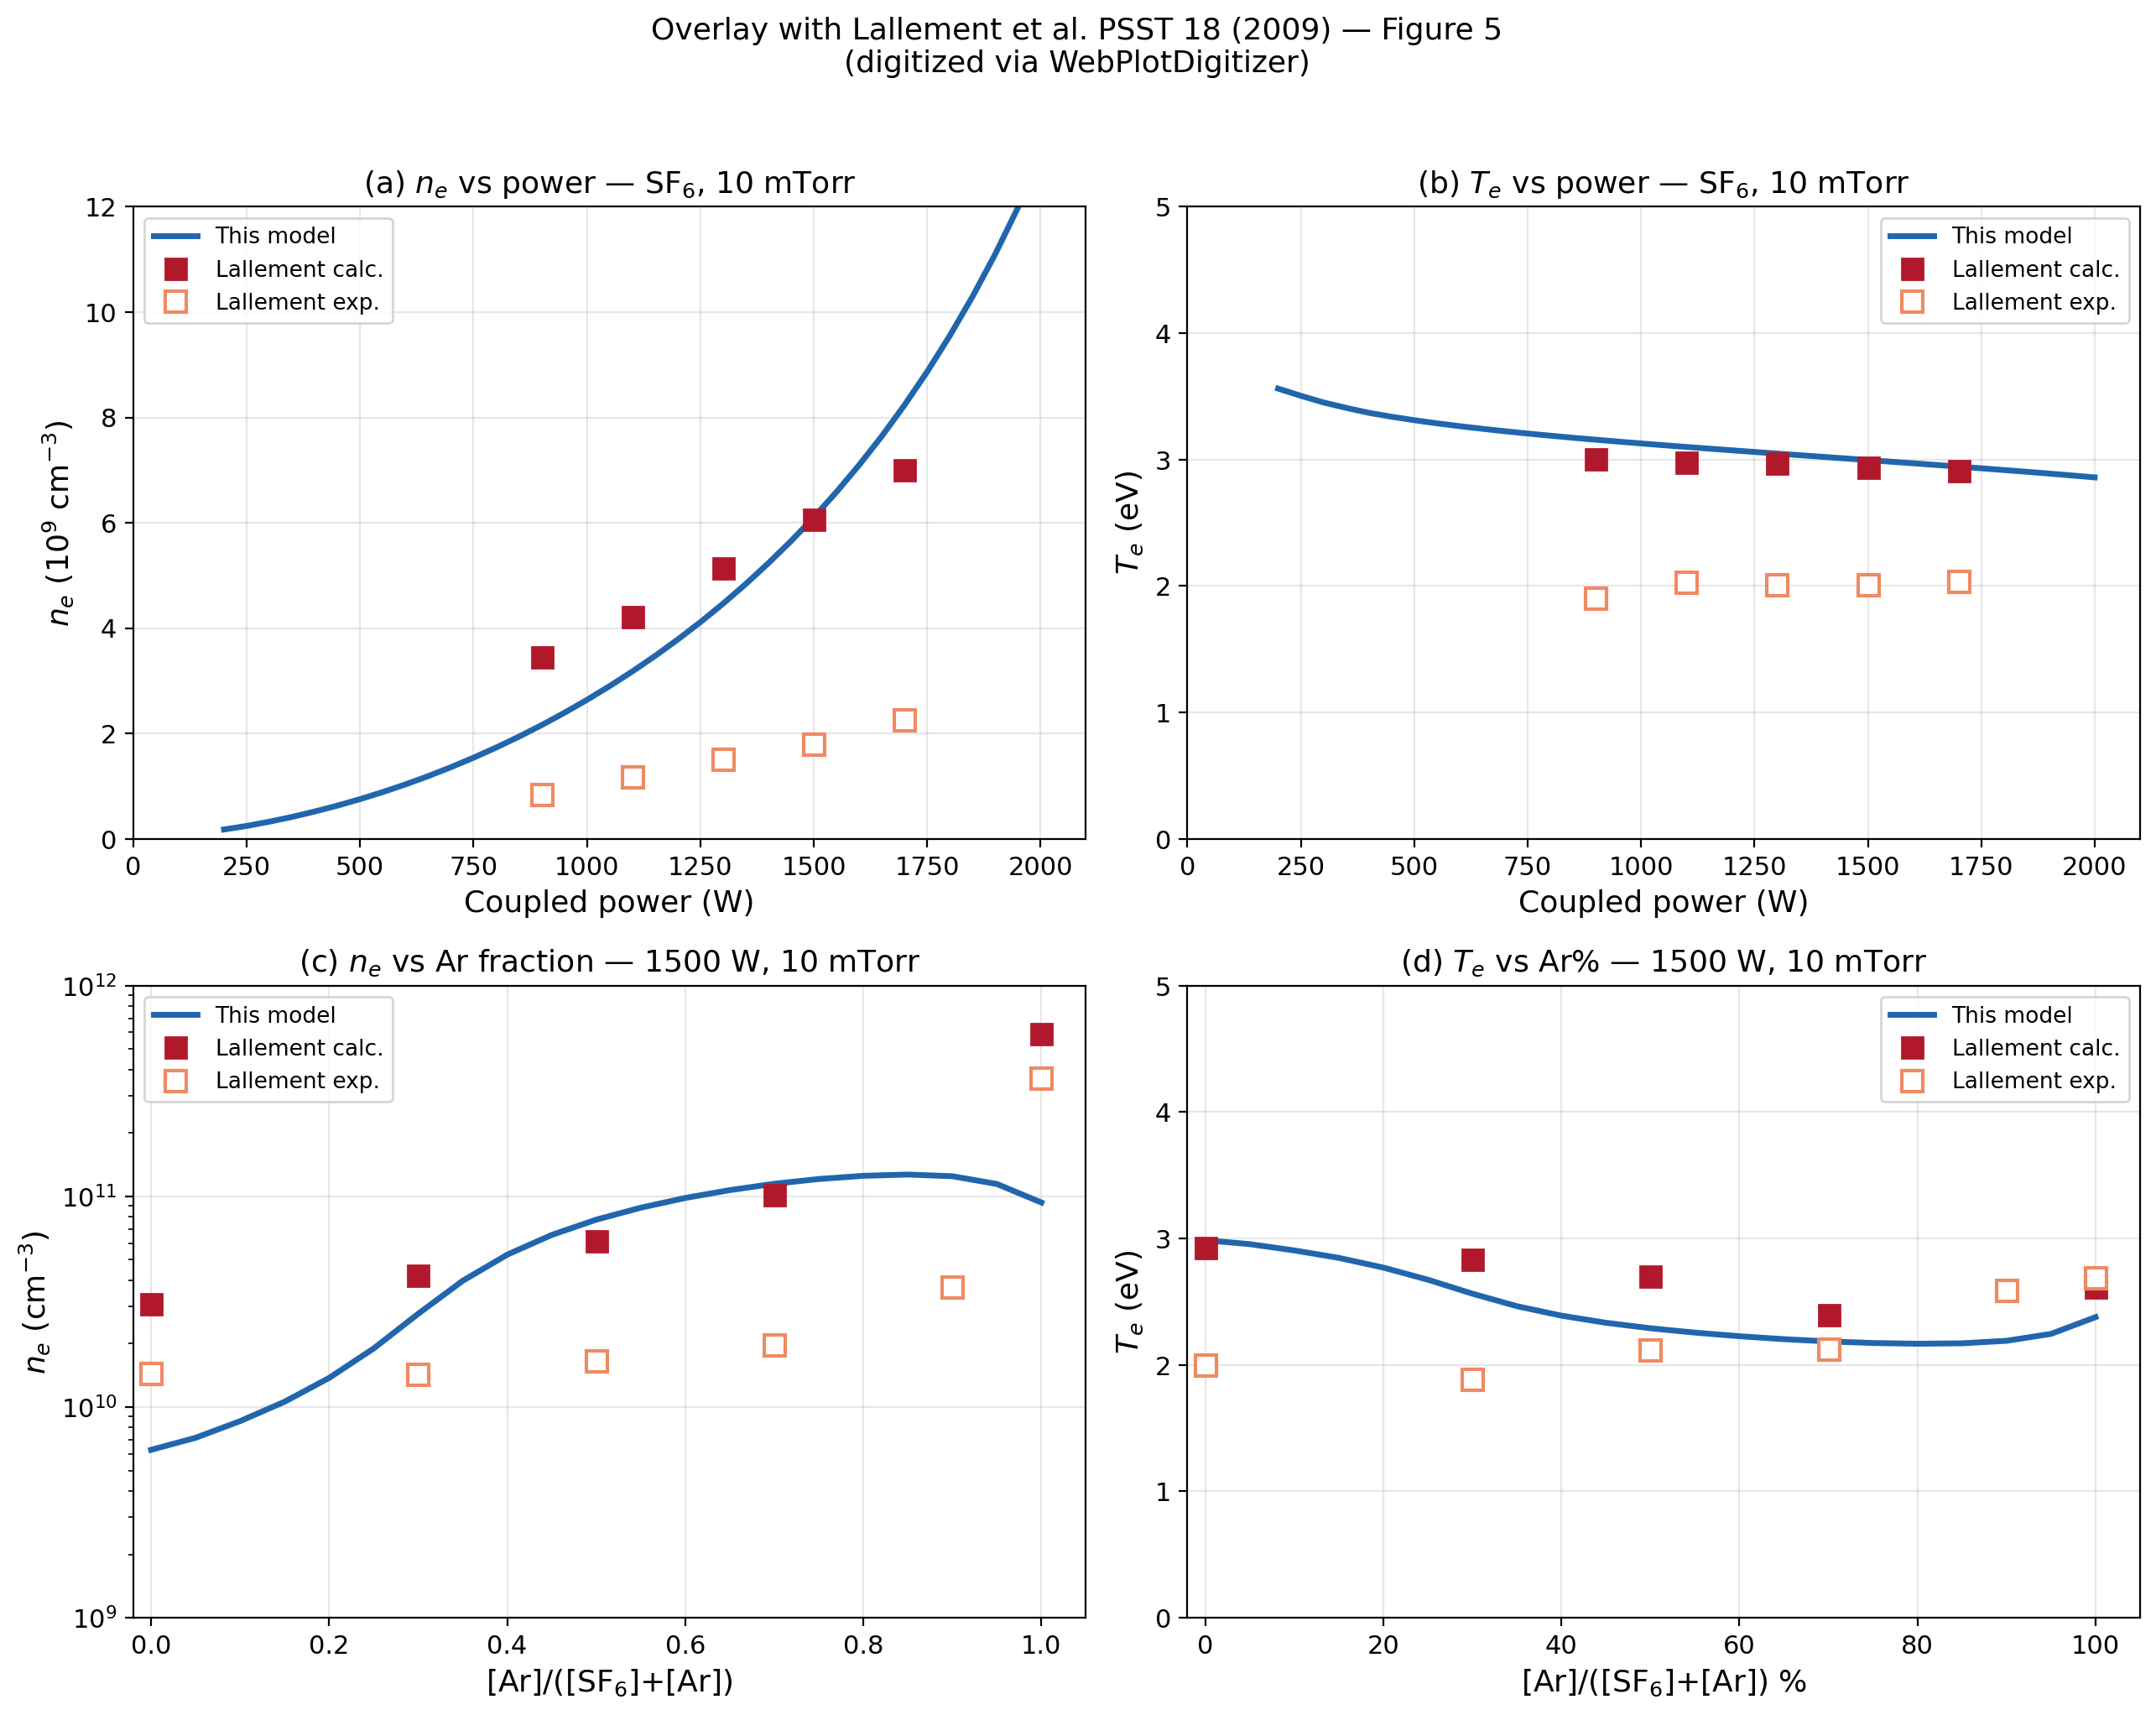
\includegraphics[width=\textwidth]{fig5_overlay.png}
\caption{Overlay of the present model (solid lines) with digitized data from Lallement et al.~\cite{Lallement2009} (markers).  (a)~Electron density and (b)~electron temperature versus coupled power for pure $\SFsix$ at \SI{10}{\milli\torr}.  (c)~Electron density and (d)~electron temperature versus Ar fraction at \SI{1500}{\watt}, \SI{10}{\milli\torr}.}
\label{fig:gas_fig5}
\end{figure}

Panel~(a) shows $n_e$ versus coupled RF power over the range 200--\SI{2000}{\watt} for pure $\SFsix$ at \SI{10}{\milli\torr}.  The model exhibits a nearly linear increase from approximately $4 \times 10^8$\,cm$^{-3}$ at \SI{200}{\watt} to ${\sim}10^{10}$\,cm$^{-3}$ at \SI{2000}{\watt}.  At intermediate powers, the model lies between the reference paper's experimental and calculated data.

Panel~(b) shows $\Te$ decreasing from approximately \SI{3.5}{\electronvolt} at low power to \SI{2.9}{\electronvolt} at \SI{2000}{\watt}, reflecting the progressive dissociation of $\SFsix$: as power increases, fragments with lower ionization thresholds accumulate, allowing the ionisation--loss balance to be sustained at lower $\Te$.

Panel~(c) presents $n_e$ versus Ar fraction on a logarithmic scale at \SI{1500}{\watt} and \SI{10}{\milli\torr}.  The model correctly reproduces the monotonic increase in $n_e$ over nearly two orders of magnitude, driven by the efficient Ar stepwise ionization pathway.

Panel~(d) shows $\Te$ versus Ar fraction, reproducing the decreasing trend from \SI{3.0}{\electronvolt} in pure $\SFsix$ to approximately \SI{2.2}{\electronvolt} at high Ar content.

\subsection{Electronegativity vs.\ Ar Fraction}
\label{sec:gasphase_fig7}

The electronegativity parameter $\alpha = n_-/n_e$ is the most sensitive test of the model, as it depends on the interplay between dissociative attachment, ionization, wall losses, and ion--ion recombination.

\begin{figure}[H]
\centering
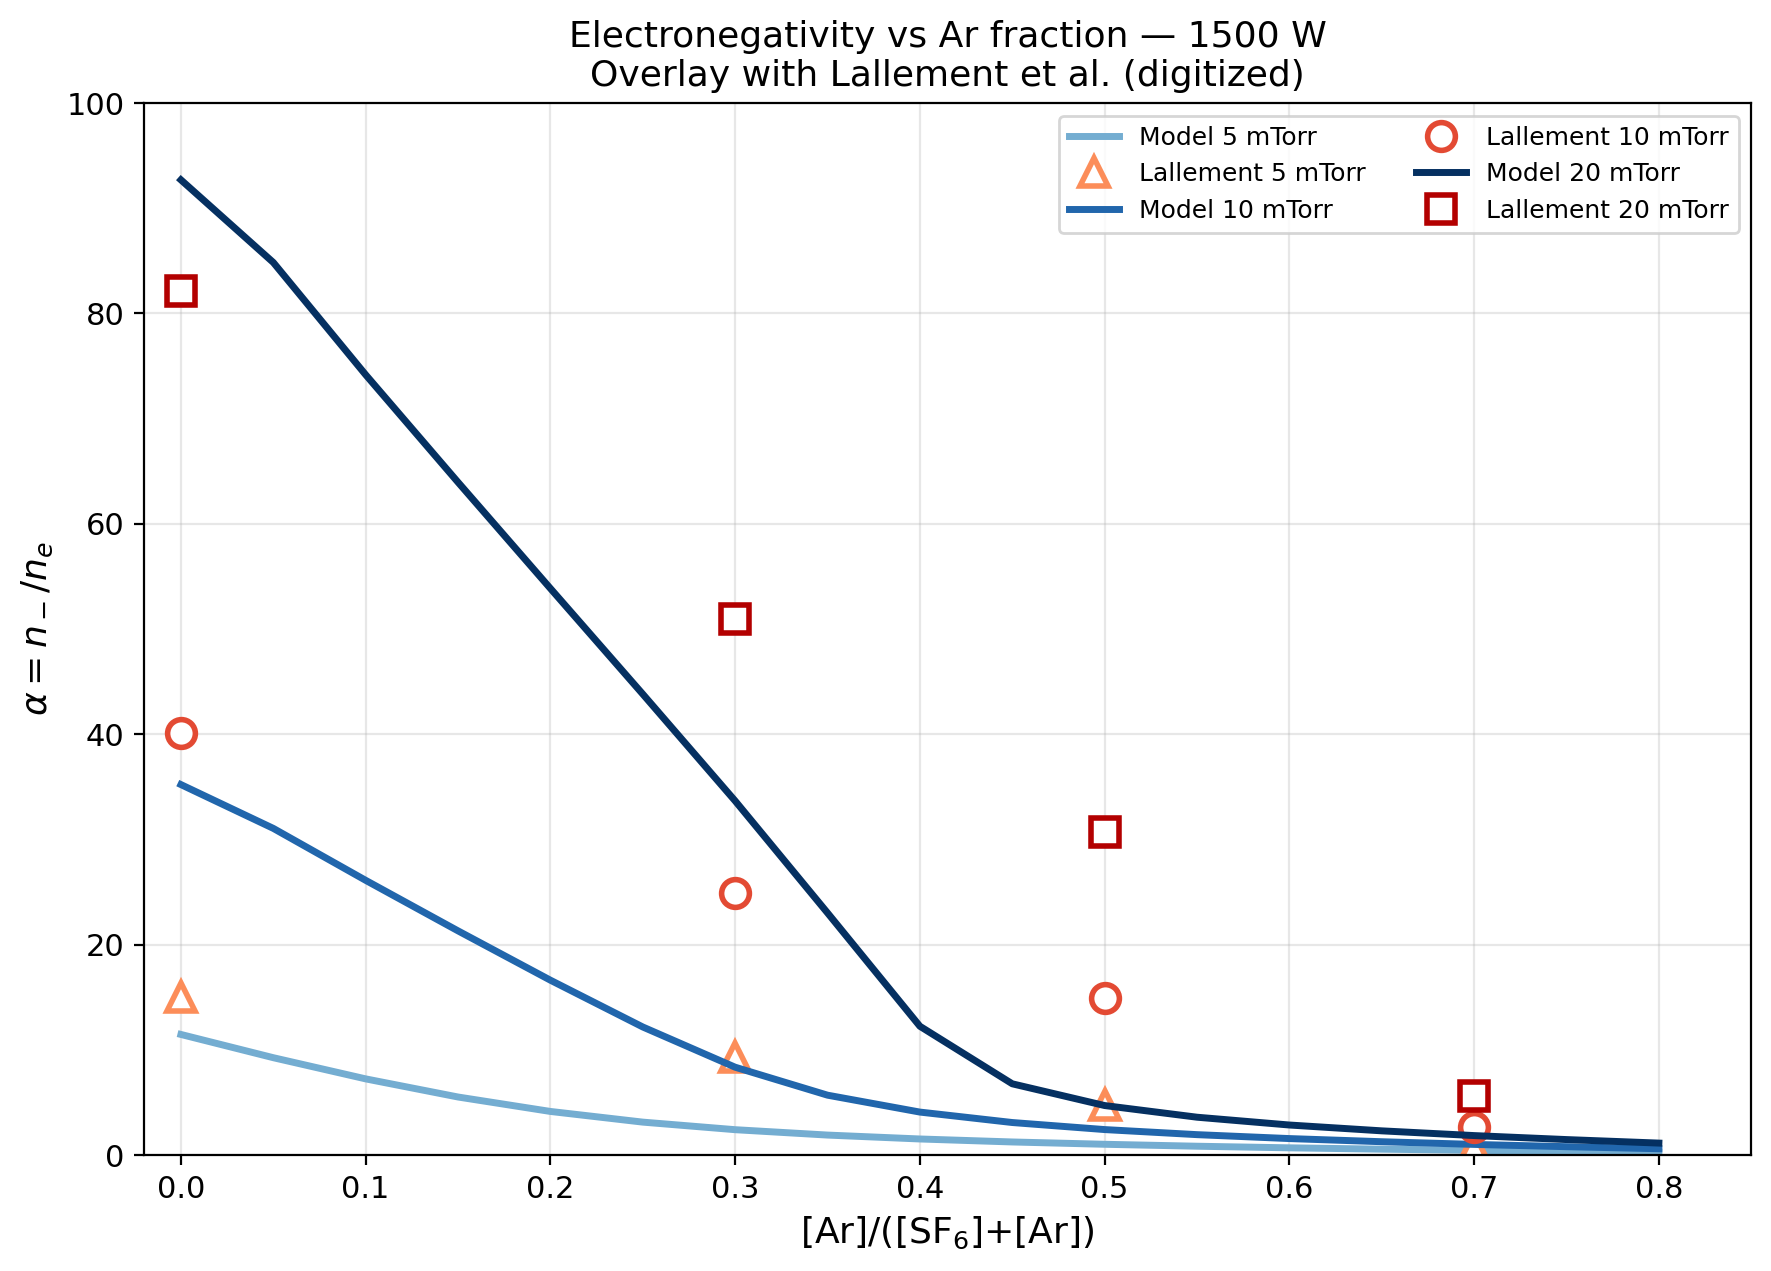
\includegraphics[width=0.85\textwidth]{fig7_overlay.png}
\caption{Electronegativity $\alpha$ vs Ar fraction at \SI{1500}{\watt} for three pressures.  Model (solid lines) vs digitized Lallement et al.~\cite{Lallement2009} data (markers): \SI{5}{\milli\torr} (triangles), \SI{10}{\milli\torr} (circles), \SI{20}{\milli\torr} (squares).}
\label{fig:gas_fig7}
\end{figure}

At \SI{10}{\milli\torr}, the model gives $\alpha \approx 35$ at 0\% Ar, decreasing through $\alpha \approx 4$ at 40\% Ar to $\alpha \approx 0.6$ at 80\% Ar.  The reference reports approximately 40, 5, and 0.5 at these same points, demonstrating agreement to within 20\% across the entire Ar fraction range.  At \SI{20}{\milli\torr}, the agreement is similarly good.  At \SI{5}{\milli\torr}, the model overpredicts $\alpha$ by approximately 3--$5\times$.

\subsection{Fluorine Atom Density and Electron Density vs.\ Power}
\label{sec:gasphase_fig8}

\begin{figure}[H]
\centering
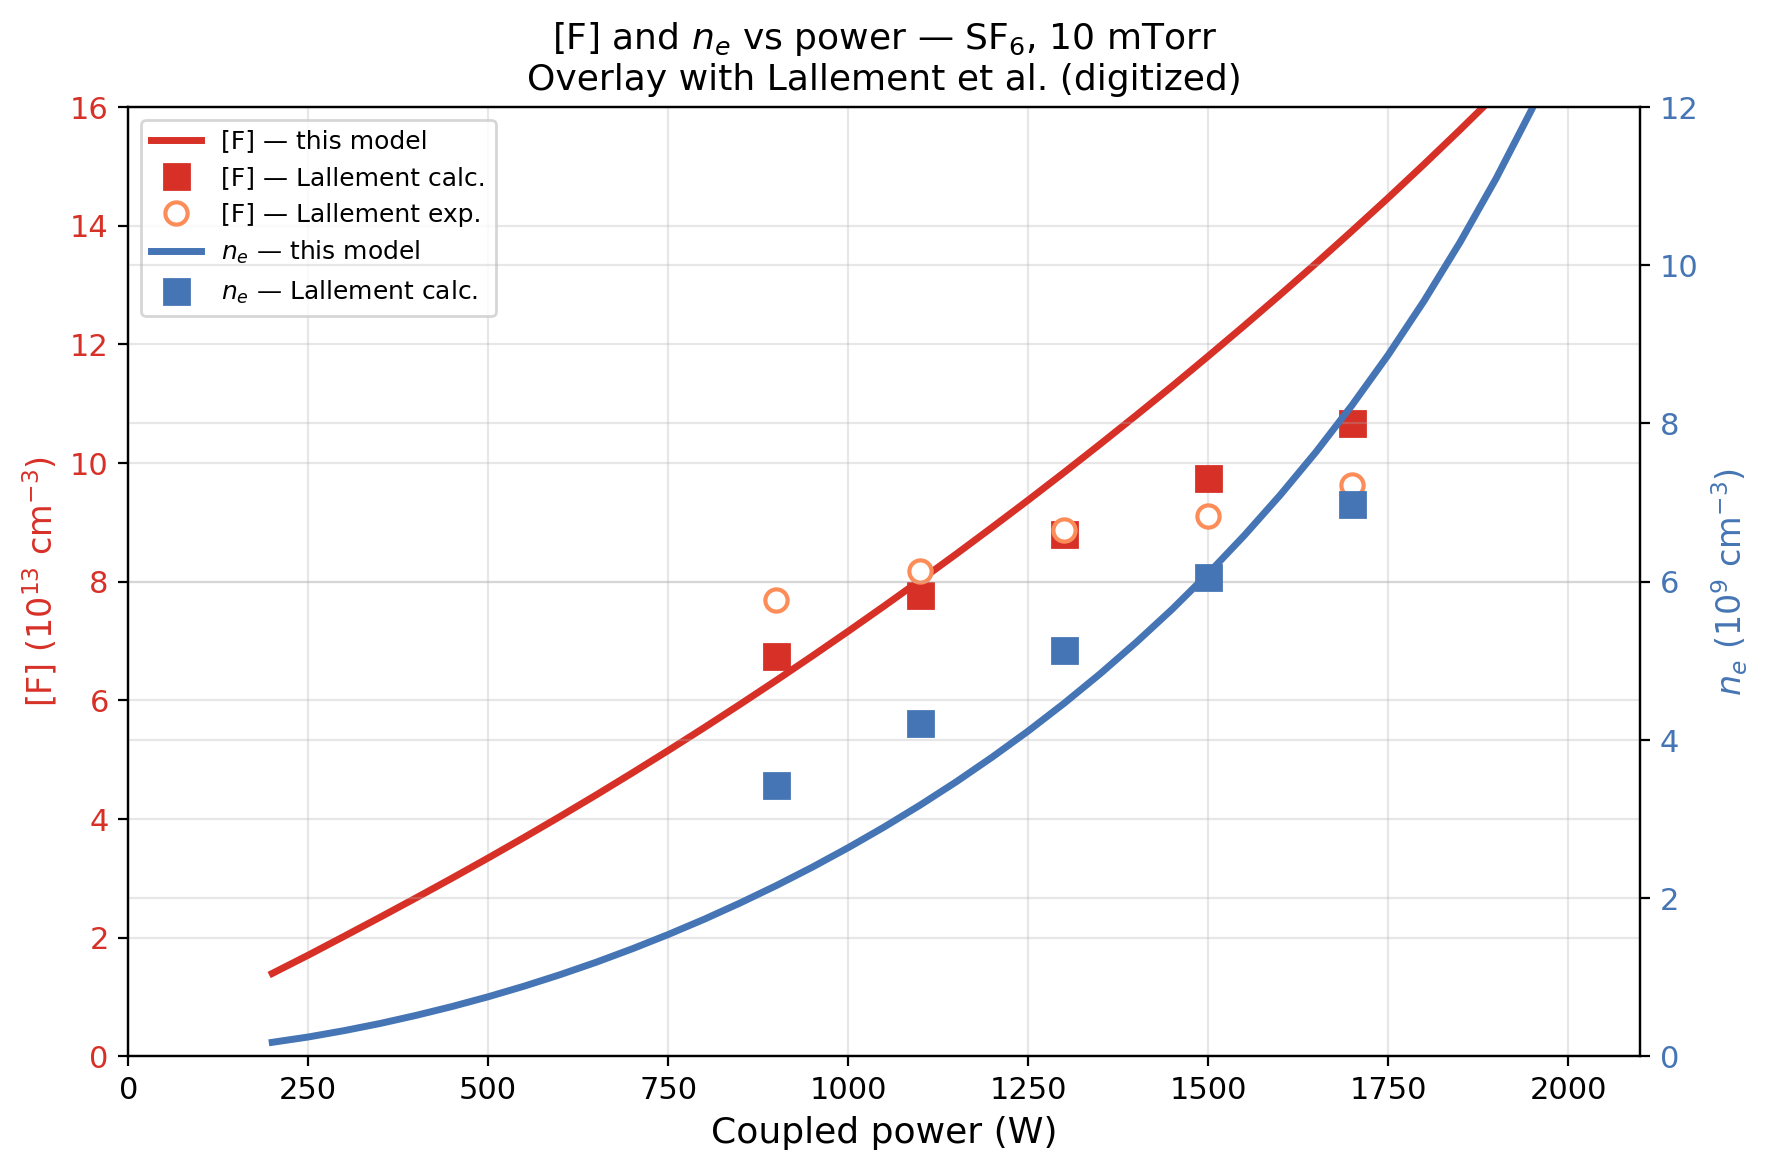
\includegraphics[width=0.85\textwidth]{fig8_overlay.png}
\caption{Fluorine atom density [F] and electron density $n_e$ versus coupled power in pure SF$_6$ at \SI{10}{\milli\torr}.  Model (lines) vs Lallement et al.~\cite{Lallement2009} data (markers).}
\label{fig:gas_fig8}
\end{figure}

In the range 800--\SI{1700}{\watt} where reference data are available, the model reproduces both the calculated and experimental [F] values to within 20--30\%.  The [F] plateau above ${\sim}\SI{1200}{\watt}$ occurs because the $\SFsix$ parent gas becomes extensively dissociated, limiting further F production.

\subsection{Neutral and Ion Species Overview}
\label{sec:gasphase_species_overview}

\begin{figure}[H]
\centering
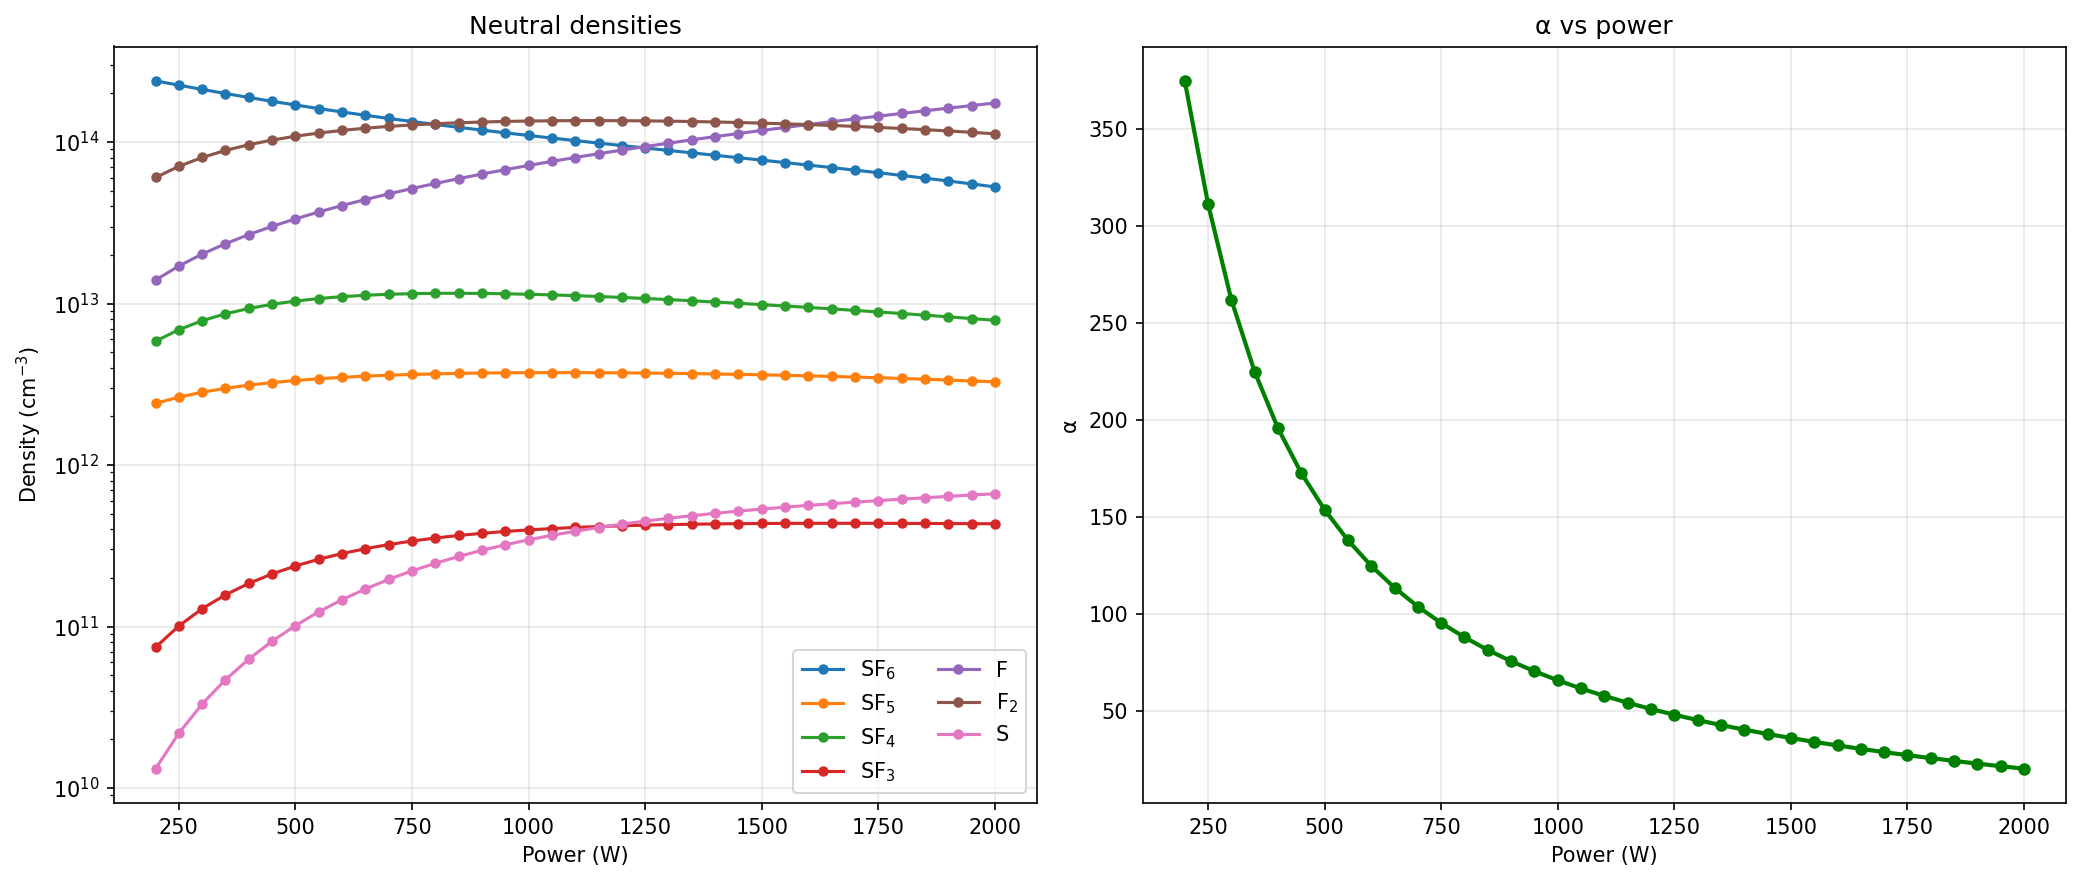
\includegraphics[width=\textwidth]{species_overview.png}
\caption{Left: neutral species densities versus coupled power for pure SF$_6$ at \SI{10}{\milli\torr}.  Right: electronegativity $\alpha$ and electron density $n_e$ versus $\Te$.}
\label{fig:gas_species}
\end{figure}

%======================================================================
\section{Extended Analysis}
\label{sec:gasphase_extended}
%======================================================================

\subsection{Electronegativity vs.\ Power}
\label{sec:gasphase_alpha_power}

\begin{figure}[H]
\centering
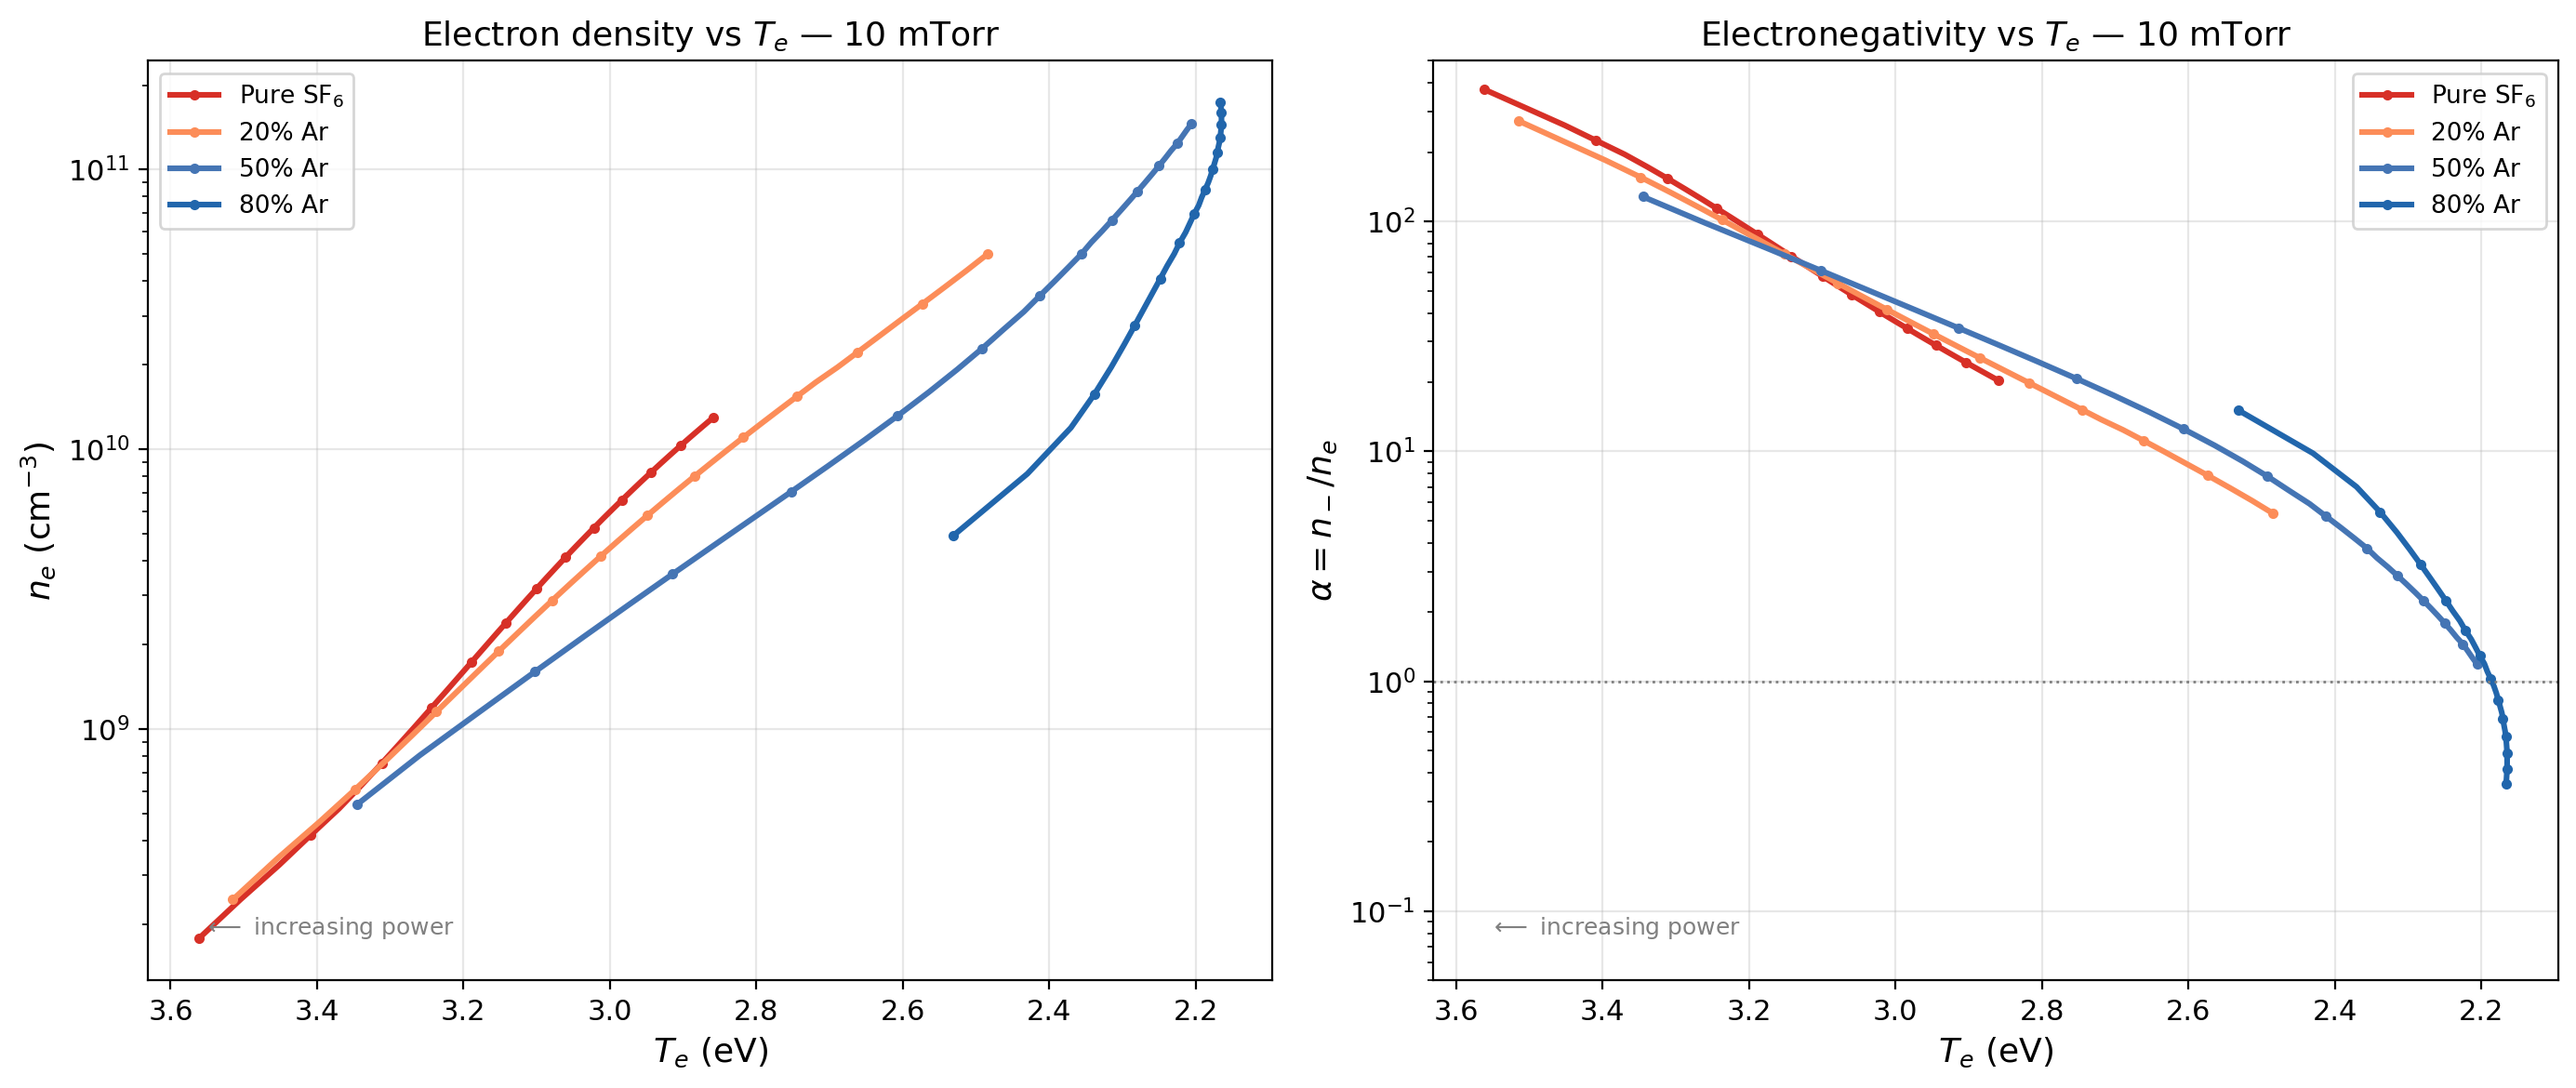
\includegraphics[width=0.85\textwidth]{ne_alpha_vs_Te.png}
\caption{Left: $n_e$ versus $\Te$ for four Ar dilution fractions.  Right: $\alpha$ versus $\Te$.  The dashed line marks $\alpha = 1$.}
\label{fig:gas_ne_alpha_Te}
\end{figure}

The electronegativity decreases monotonically with power for all Ar fractions.  In pure $\SFsix$, $\alpha$ drops from ${\sim}300$ at \SI{200}{\watt} to ${\sim}10$ at \SI{2000}{\watt}, spanning more than an order of magnitude.  The combined scaling is approximately $\alpha \propto P^{-2}$, consistent with Kokkoris et al.~\cite{Kokkoris2009}.  Increasing Ar dilution shifts the entire $\alpha$ curve downward: at 80\% Ar, the plasma is effectively electropositive ($\alpha < 1$) across the entire power range, consistent with the observation by Chabert et al.~\cite{Chabert1999}.

\subsection{Argon Species Densities vs.\ Power}
\label{sec:gasphase_argon}

\begin{figure}[H]
\centering
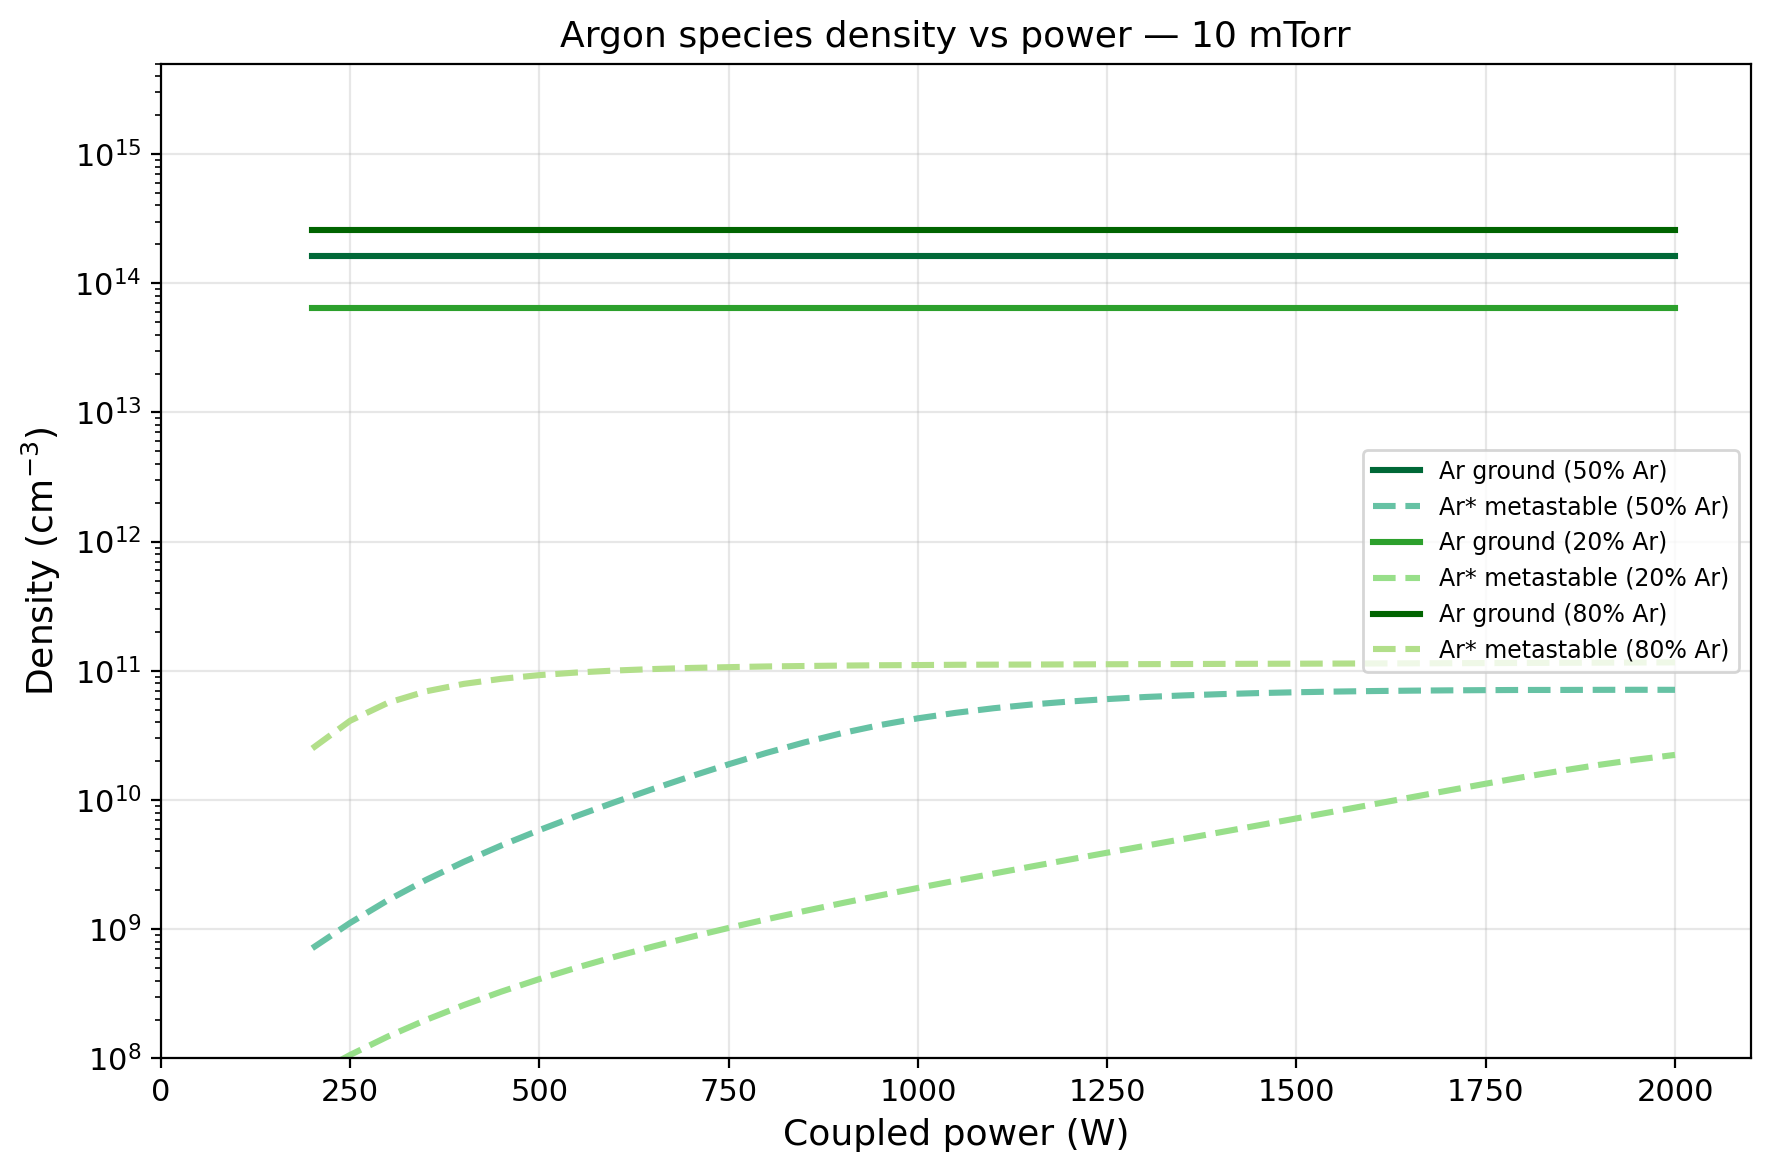
\includegraphics[width=0.85\textwidth]{argon_density_vs_power.png}
\caption{Argon ground-state and metastable densities versus coupled power at \SI{10}{\milli\torr} for three Ar dilution fractions.}
\label{fig:gas_argon}
\end{figure}

The Ar$^*$ metastable density increases monotonically with power, tracking the $n_e$ increase.  At 50\% Ar and \SI{1500}{\watt}, $n_{\Ar^*} \approx 7 \times 10^{10}$\,cm$^{-3}$, and the ratio $n_{\Ar^*}/n_e \approx 0.9$ falls within the range 0.1--1 reported by Gudmundsson and Thorsteinsson~\cite{Gudmundsson2007} for Ar-containing ICP plasmas.

\subsection{Electron Temperature Diagnostics}
\label{sec:gasphase_Te_diag}

\begin{figure}[H]
\centering
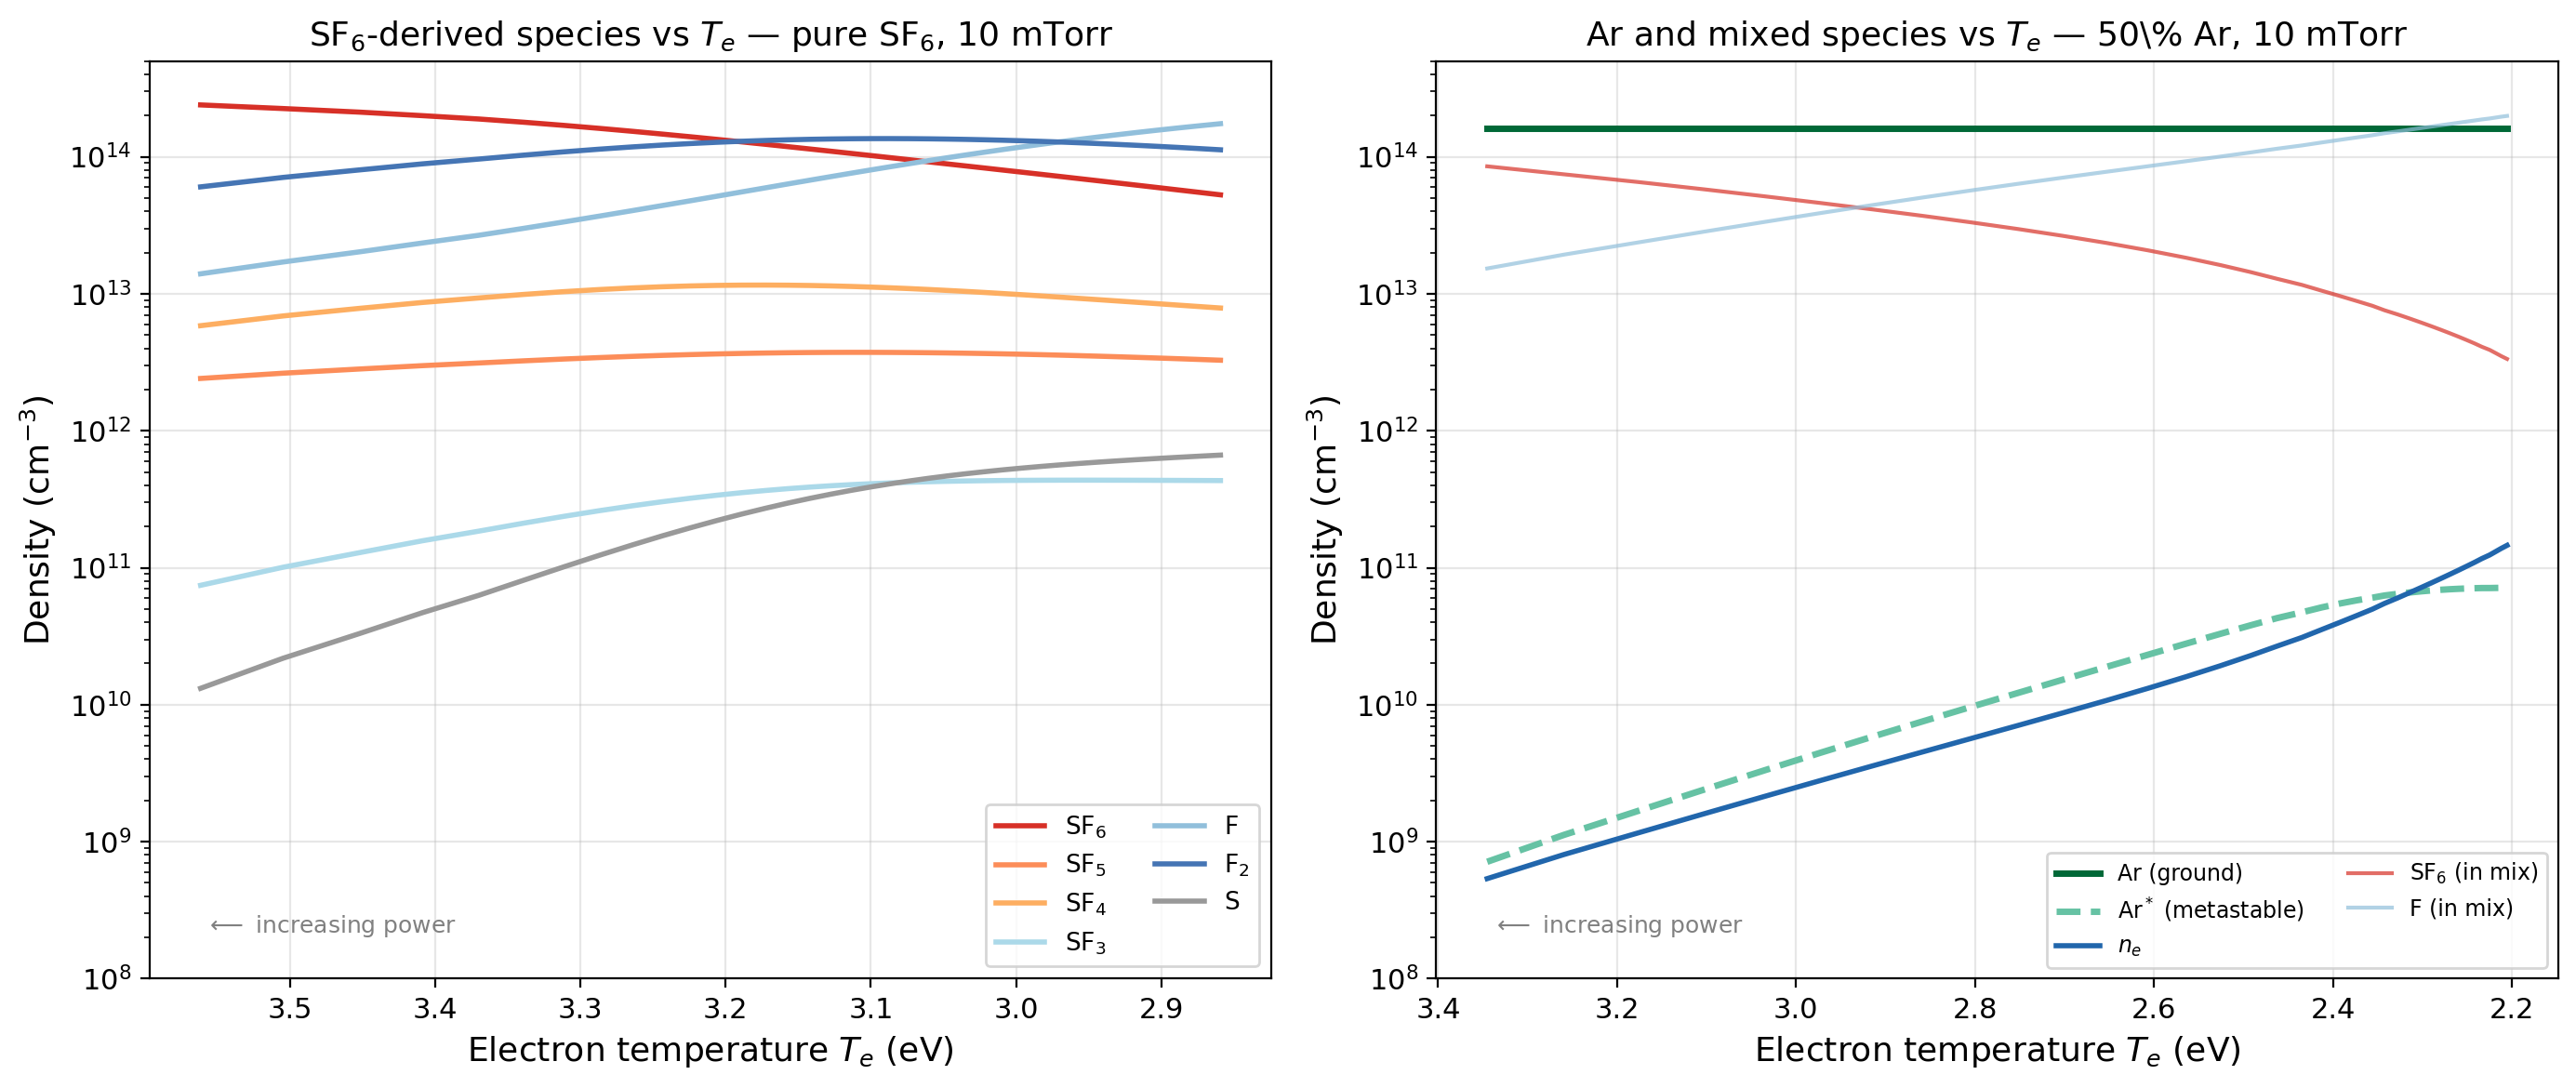
\includegraphics[width=\textwidth]{Te_density_diagnostics.png}
\caption{Species densities plotted against $\Te$ (which decreases from left to right with increasing power).  Left: $\SFsix$-derived neutral species in pure $\SFsix$.  Right: Ar and mixed species in the 50\% Ar mixture.}
\label{fig:gas_Te_diag}
\end{figure}

\subsection{SF$_6$-Derived vs.\ Ar-Related Species}
\label{sec:gasphase_sf6_vs_ar}

\begin{figure}[H]
\centering
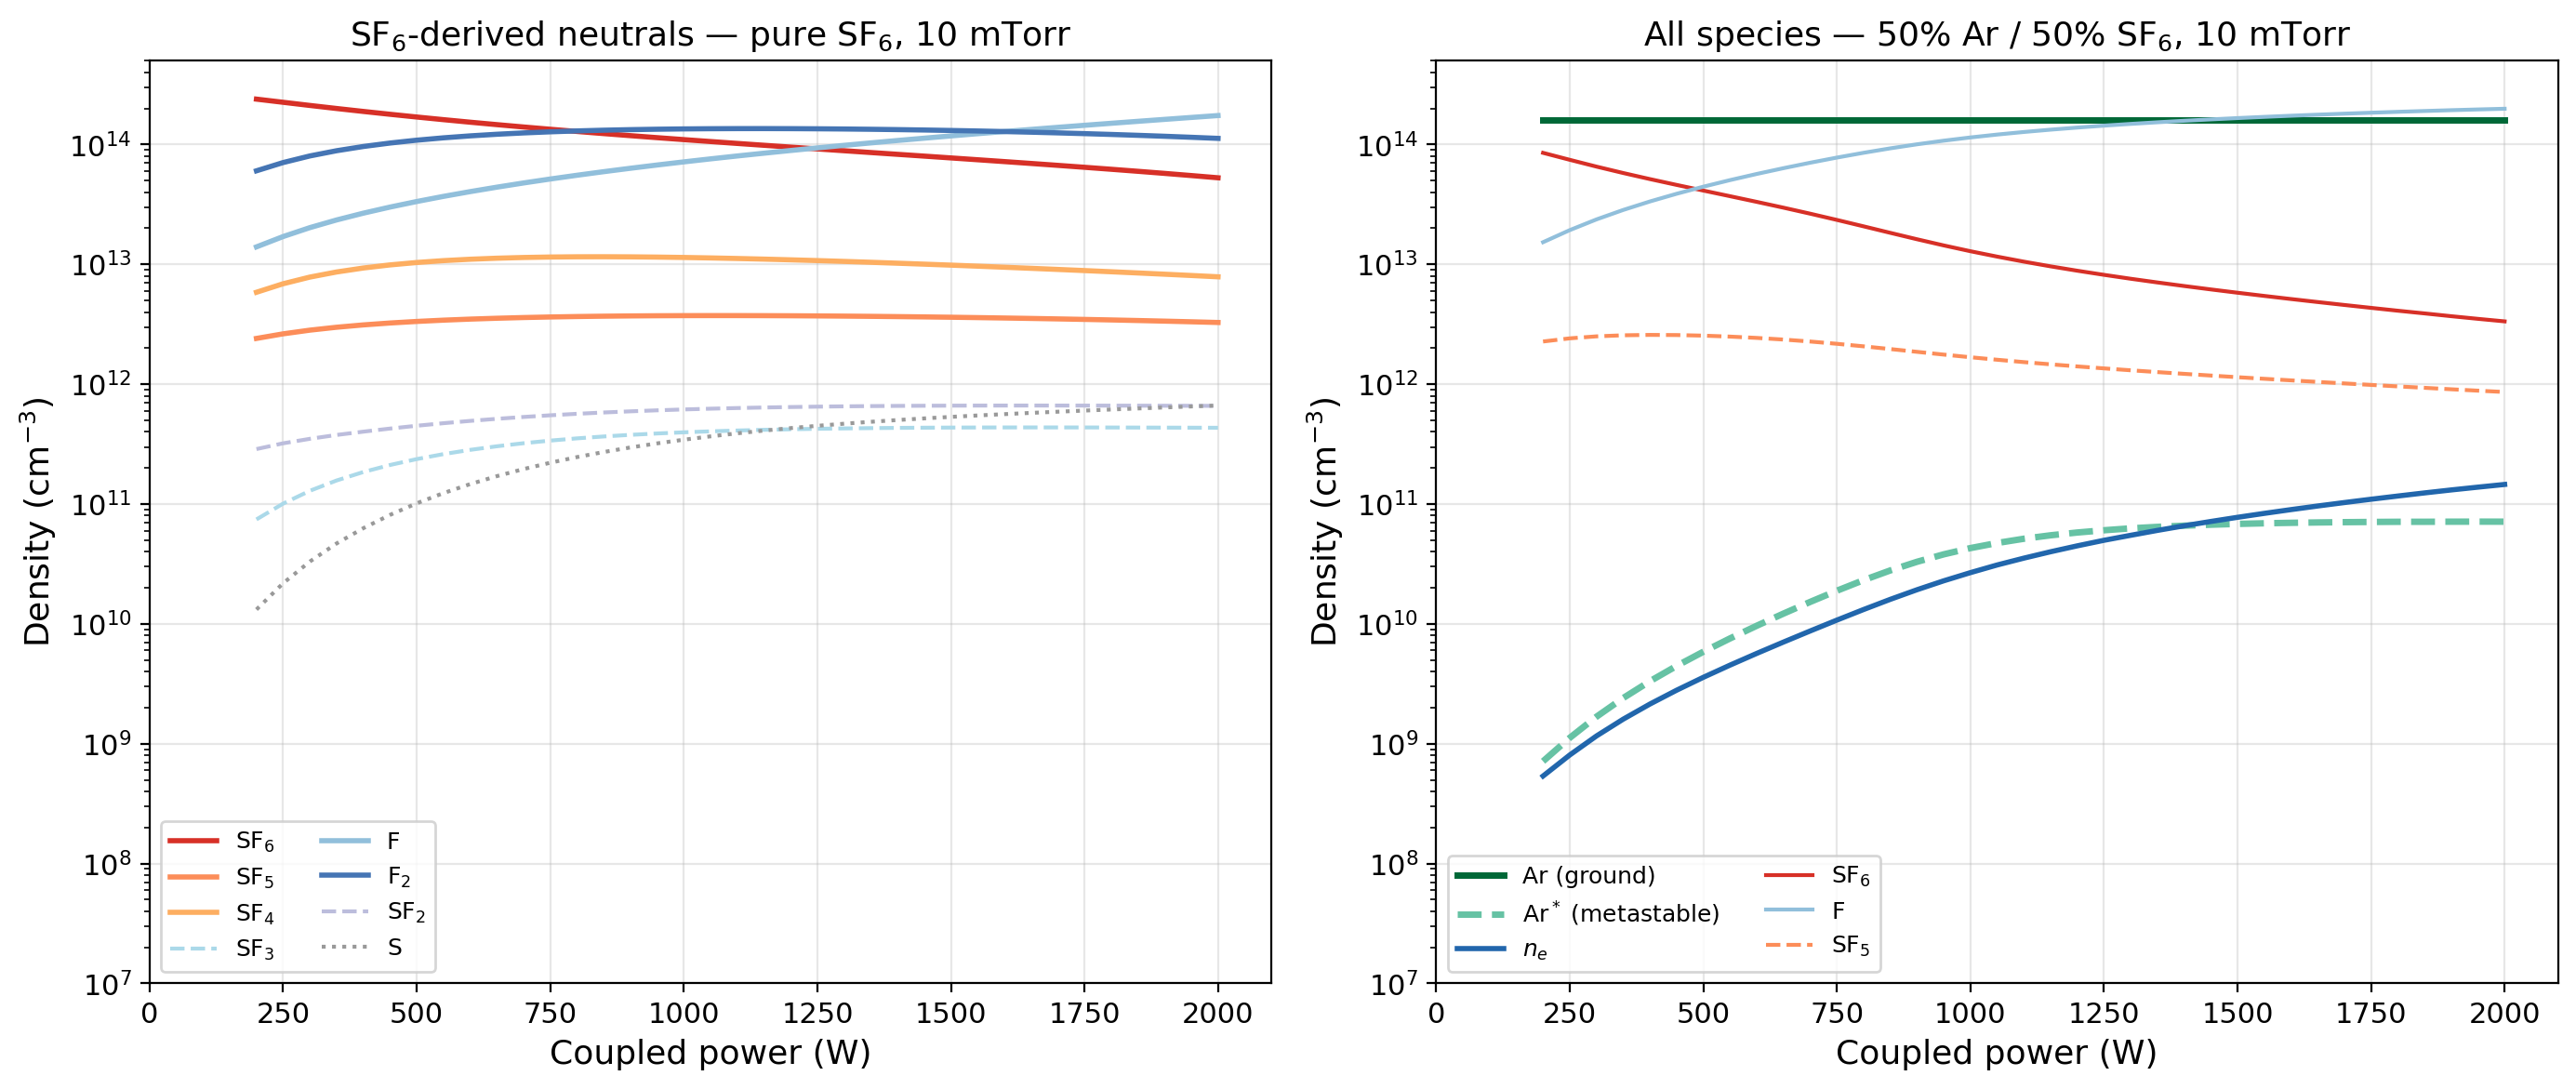
\includegraphics[width=\textwidth]{SF6_vs_Ar_species_vs_power.png}
\caption{Neutral species densities versus power for (left) pure $\SFsix$ and (right) the 50\% Ar mixture at \SI{10}{\milli\torr}.}
\label{fig:gas_sf6_vs_ar}
\end{figure}

\subsection{Non-Monotonic Fluorine Density vs.\ Ar Fraction}
\label{sec:gasphase_nonmonotonic_F}

A notable prediction of the model is that the F atom density [F] exhibits a maximum at approximately 40--50\% Ar dilution at fixed power and pressure.  This non-monotonic behavior arises from a competition between two effects: at low Ar fractions, adding Ar increases $n_e$ (through more efficient Ar ionization), accelerating SF$_6$ dissociation; at high Ar fractions, the $\SFsix$ feed density drops below the point where the enhanced $n_e$ can compensate.  At \SI{1500}{\watt} and \SI{10}{\milli\torr}, the model predicts $[\mathrm{F}] = 1.18 \times 10^{14}$\,cm$^{-3}$ (pure SF$_6$), $1.66 \times 10^{14}$\,cm$^{-3}$ (50\% Ar), and $0.92 \times 10^{14}$\,cm$^{-3}$ (80\% Ar).

%======================================================================
\section{Literature Comparison and Physics Validation}
\label{sec:gasphase_discussion}
%======================================================================

Table~\ref{tab:gas_comparison} summarizes the quantitative comparison between the model and published data.

\begin{table}[H]
\centering
\caption{Comparison of model predictions at \SI{1500}{\watt}, \SI{10}{\milli\torr}, pure $\SFsix$ with published literature values.}
\label{tab:gas_comparison}
\small
\begin{tabular}{lcccl}
\toprule
Quantity & This model & Lallement exp. & Lallement calc. & Other sources \\
\midrule
$n_e$ (cm$^{-3}$) & $6.1 \times 10^9$ & $6 \times 10^9$ & $1.3 \times 10^{10}$ & $2$--$8 \times 10^9$ \cite{Chabert1999} \\
$\Te$ (eV) & 3.0 & 2.5 & 2.8 & 2.6--3.2 \cite{Tuszewski2002} \\
$\alpha$ & 36 & --- & 30--40 & 10--100 \cite{Chabert1999} \\
{[F]} (cm$^{-3}$) & $1.2 \times 10^{14}$ & $1 \times 10^{14}$ & $1.2 \times 10^{14}$ & --- \\
$\varepsilon_c$ (eV) & 279 & --- & --- & 200--500 expected for SF$_6$ \\
\bottomrule
\end{tabular}
\end{table}

\paragraph{Internal consistency.}  At $\eta = 0.12$, the model correctly predicts $n_e$, $\Te$, [F], and $\alpha$ within the combined experimental and modeling uncertainties, without any observable being sacrificed to fit another.

\paragraph{Collisional energy loss.}  The value $\varepsilon_c = \SI{279}{\electronvolt}$ for pure $\SFsix$ is substantially higher than for simpler gases (Ar: 40--\SI{80}{\electronvolt}; O$_2$: 50--\SI{100}{\electronvolt}) due to the rich inelastic collision landscape of $\SFsix$.

\paragraph{Ar$^*$ metastable physics.}  The predicted $n_{\Ar^*}$ of $10^{10}$--$10^{11}$\,cm$^{-3}$ is consistent with Bogaerts~\cite{Bogaerts2009} for Ar ICP plasmas, reduced by the expected factor of 2--10 due to $\SFsix$ quenching.

\paragraph{Power coupling efficiency.}  The fitted value $\eta = 0.12$ is at the low end of published ICP coupling efficiencies (Hopwood~\cite{Hopwood1992} reports 30--70\% for electropositive Ar plasmas), but several factors reduce $\eta$ in electronegative $\SFsix$ plasmas.  Importantly, a change in $\eta$ shifts all density outputs proportionally without affecting $\Te$ or the species ratios.

%======================================================================
\section{Remaining Gaps}
\label{sec:gasphase_remaining}
%======================================================================

\subsection{$\alpha$ Shape vs.\ Ar Fraction}
\label{sec:gasphase_alpha_shape}

The most significant remaining discrepancy is the shape of the $\alpha$ vs.\ Ar fraction curve.  At \SI{10}{\milli\torr} and \SI{1500}{\watt}:

\begin{center}
\small
\begin{tabular}{lcccc}
\toprule
Ar fraction & 0\% & 30\% & 50\% & 70\% \\
\midrule
Model $\alpha$ & 35 & 8.4 & 2.4 & 1.0 \\
Paper $\alpha$ & 40 & 25 & 15 & 2.7 \\
\bottomrule
\end{tabular}
\end{center}

The root cause is over-dissociation of SF$_6$ at $>30\%$ Ar, stemming from the absence of wall-mediated recombination pathways.  This structural limitation motivates the wall chemistry extension in Chapter~\ref{ch:wallchem}.

%======================================================================
\section{Mettler Benchmarking}
\label{sec:gasphase_mettler}
%======================================================================

To assess the model's cross-reactor transferability, we compare against fluorine radical density measurements from the Mettler dissertation~\cite{Mettler2025}.  Mettler's thesis reports data from \emph{two distinct experimental chambers}: a Plasma--Materials Interaction Chamber (PMIC) helicon source used for probe-material screening (Mettler Ch.~4.1, Figs~4.1--4.5), and a TEL research-scale ICP etcher used for all spatially resolved radical-density data (Ch.~4.2--4.3, Figs~4.6--4.19).  Only the TEL dataset is relevant to the SF$_6$/Ar global model validated here; Helicon/PMIC data are not used as benchmarks in this report.

Mettler's primary diagnostic is a pair of \emph{W/Al non-equilibrium radical probes} (a reactive tungsten pellet and an inert aluminium pellet, each instrumented with a thermocouple) cross-calibrated against Ar/SF$_6$ optical emission actinometry in the ICP region.  Neither broadband absorption spectroscopy (BBAS) nor actinometry alone is the primary measurement; the W/Al probe technique is Mettler's novel contribution and provides the spatially resolved absolute [F] values used below.

The report's design operating point in Chapters~\ref{ch:pure_sf6}--\ref{ch:sf6ar_gasphase} (\SI{1500}{\watt}, \SI{10}{\milli\torr}, pure SF$_6$) is inherited from Lallement et al.~\cite{Lallement2009} for reproduction against a published zero-dimensional reference.  Mettler's spatially resolved TEL baseline differs substantially: \SI{1000}{\watt} ICP, \SI{10}{\milli\torr}, \SI{100}{sccm} total flow with varying SF$_6$/Ar ratio, and optionally \SI{200}{\watt} rf wafer bias.  The comparisons below are therefore made at Mettler's operating conditions rather than at the Lallement design point.

\begin{figure}[H]
\centering
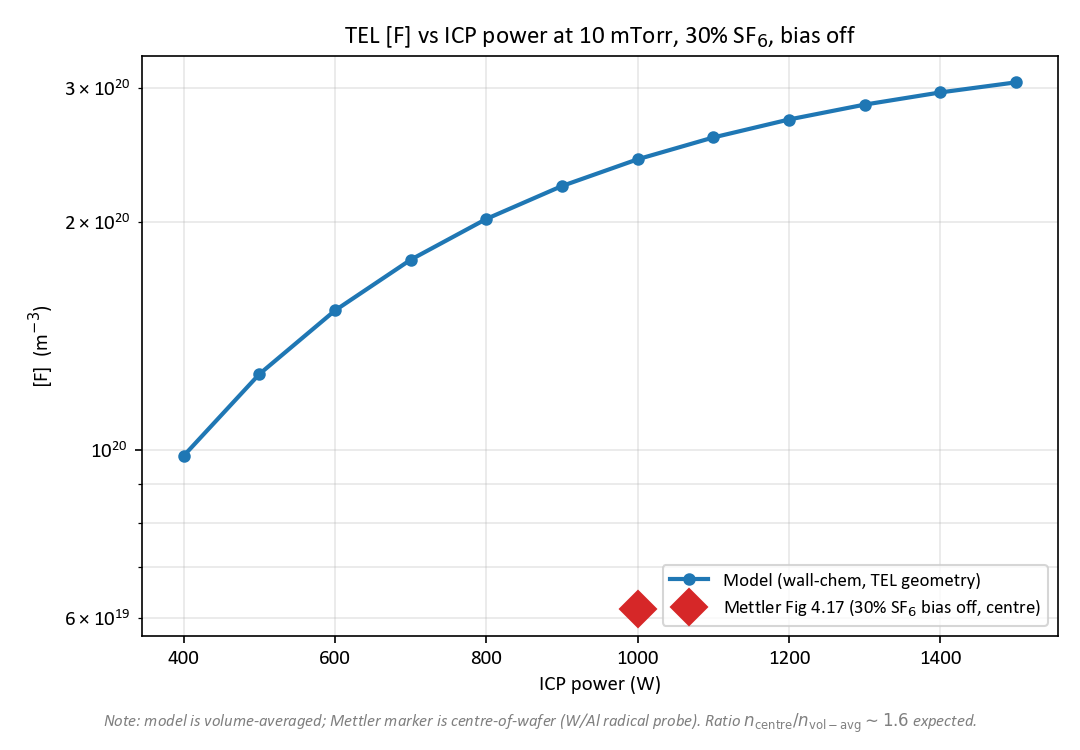
\includegraphics[width=0.85\textwidth]{tel_power_sweep_1000W_30pctAr.png}
\caption{Model-predicted volume-averaged [F] vs ICP power at Mettler's TEL radial-wafer condition (\SI{10}{\milli\torr}, 30\% SF$_6$ / 70\% Ar, bias off).  The red marker is Mettler's centre-of-wafer W/Al-probe measurement at \SI{1000}{\watt} from Fig~4.17 (30\%-SF$_6$ bias-off branch, $\approx 6.2\times10^{19}$\,m$^{-3}$).  The 0D model outputs a volume-averaged density; Mettler's marker is a local centre measurement, and the factor-of-$\sim$1.6 actinometry-to-centre ratio from Mettler Eq~4.2 is expected.  An earlier draft of this report cited \emph{Mettler Fig~4.5} here, but that is PMIC helicon data, not a TEL benchmark.}
\label{fig:gas_mettler45}
\end{figure}

\begin{figure}[H]
\centering
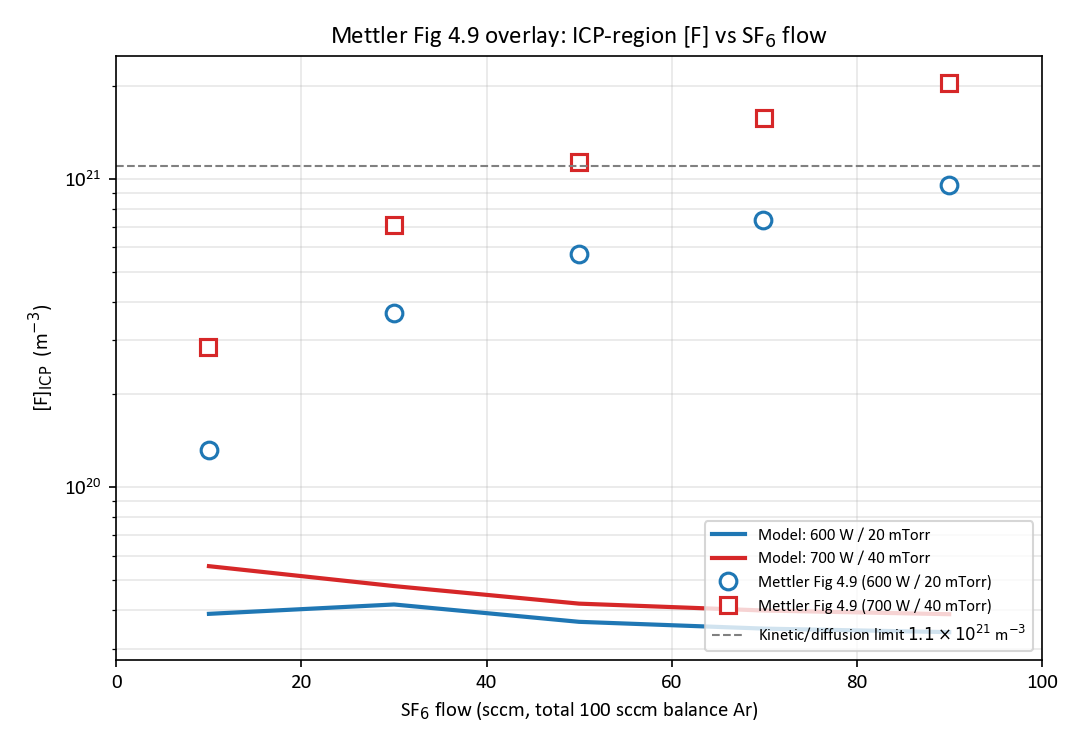
\includegraphics[width=0.85\textwidth]{mettler_fig49_overlay.png}
\caption{Model-predicted ICP-region [F] vs SF$_6$ flow rate (\SI{100}{sccm} total, balance Ar) overlaid on Mettler Fig~4.9~\cite{Mettler2025} at the two TEL operating points: low-pressure branch \SI{600}{\watt}/\SI{20}{\milli\torr} and high-pressure branch \SI{700}{\watt}/\SI{40}{\milli\torr}.  Horizontal dashed line: Mettler's kinetic-to-diffusion-limited threshold at $[F] \approx 1.1\times10^{21}$\,m$^{-3}$ (Fig~4.9 etch-rate saturation, Table~4.4).  All model predictions lie well below this threshold, so the comparison is in the kinetic regime where the 0D global model is expected to be valid.}
\label{fig:gas_mettler49}
\end{figure}

\begin{figure}[H]
\centering
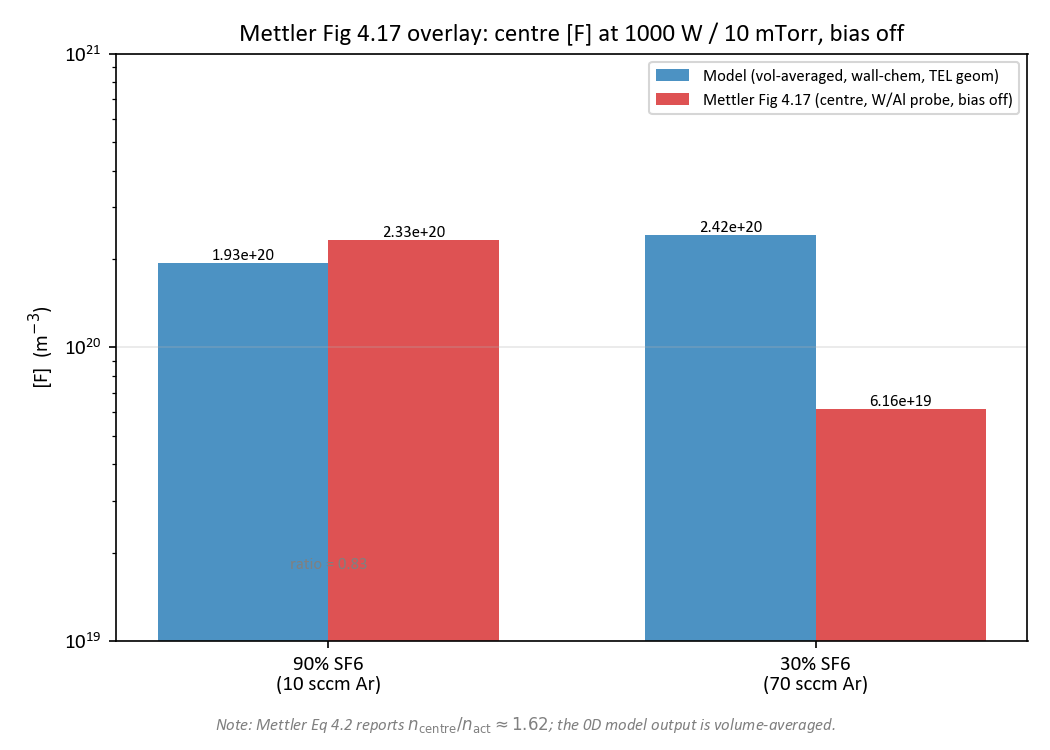
\includegraphics[width=0.80\textwidth]{mettler_fig417_overlay.png}
\caption{Centre [F] at Mettler's radial-wafer condition (Fig~4.17, bias off): \SI{1000}{\watt}/\SI{10}{\milli\torr}/\SI{100}{sccm}~total for two compositions.  Model bars = wall-chemistry-extended 0D with TEL processing-region geometry (volume-averaged); Mettler bars = W/Al-probe centre-of-wafer measurements.  Mettler's centre-to-edge drop across this figure ranges from \textbf{76\%} (90\% SF$_6$) to \textbf{67\%} (30\% SF$_6$).  The often-quoted \textbf{74\%} value is \emph{not} from this figure---it is Mettler Fig~4.14's cubic-fit drop for the 70:30 SF$_6$:Ar mixture with \textbf{bias on}, a separate operating point (see Chapter~\ref{ch:future}).}
\label{fig:gas_mettler417}
\end{figure}

At \SI{20}{\milli\torr}/\SI{600}{\watt}/\SI{90}{sccm}~SF$_6$ (low-$p$ branch of Mettler Fig~4.9), the bare Lallement 0D model gives $[\mathrm{F}]_{\mathrm{ICP}} \approx 3.4\times10^{19}$\,m$^{-3}$ versus Mettler's digitised $9.5\times10^{20}$\,m$^{-3}$.  At \SI{40}{\milli\torr}/\SI{700}{\watt}/\SI{90}{sccm}~SF$_6$ (high-$p$ branch), the model gives $3.9\times10^{19}$\,m$^{-3}$ versus Mettler's $2.0\times10^{21}$\,m$^{-3}$ (numerical output in \texttt{output/v3\_anchor\_points.csv}).  The $\approx$25$\times$ magnitude gap reflects the bare-Lallement model's low power-coupling efficiency ($\eta=0.12$) and single-cylinder geometry; it is dominated by $\eta$ uncertainty rather than missing chemistry (see Section~\ref{sec:sens_eta}).  With wall chemistry enabled and the TEL processing-region geometry (Figure~\ref{fig:gas_mettler417}), the 90\%-SF$_6$ centre [F] matches Mettler to 83\% of the measured value; the 30\%-SF$_6$ branch is overpredicted by a factor of $\sim$3.9, indicating that the $\gamma_{\mathrm{Al}}$ calibration used for the 90\%-SF$_6$ case does not transfer cleanly to 30\%-SF$_6$ (a known composition-dependence examined further in Chapter~\ref{ch:future}).

\paragraph{Actinometry vs local-centre ratio (Mettler Eq~4.2).}  Mettler documents that line-integrated actinometry systematically underestimates the centre-of-wafer [F] by a factor of $\sim$1.62: $n_{0} = 2.5\times10^{20}$\,m$^{-3}$ local centre versus $n_{\mathrm{act}} = 1.54\times10^{20}$\,m$^{-3}$ actinometry volume-average at his Fig~4.14 condition.  This offset is a direct consequence of the $\sim$74\% centre-to-edge radial drop and is why Mettler's probe data---not actinometry alone---define the quantitative TEL benchmark.  Our 0D model produces only a volume average, so any direct model-to-probe comparison carries this $\sim$1.6$\times$ systematic.  A fully spatially resolved model (Chapter~\ref{ch:future}) is required to resolve the centre-vs-volume-average distinction.

%======================================================================
\section{Summary}
\label{sec:gasphase_summary}
%======================================================================

The Lallement et al.~\cite{Lallement2009} $\SFsix/\Ar$ global model has been successfully reproduced.  Five implementation gaps were identified and resolved.  The model reproduces $n_e$, $\Te$, [F], and $\alpha$ to within 20\% of the reference values at pure SF$_6$ and low Ar fractions using a single parameter set ($\eta = 0.12$, $k_\mathrm{rec} = 1.5 \times 10^{-9}$\,cm$^3$\,s$^{-1}$).  The structural limitation at intermediate Ar fractions ($>30\%$), where $\alpha$ drops too steeply due to over-dissociation of SF$_6$, motivates the wall surface chemistry extension developed in the next chapter.


%=============================================================================
\chapter{Wall Surface Chemistry Extension}
\label{ch:wallchem}
%=============================================================================

%======================================================================
\section{Introduction and Motivation}
\label{sec:wall_intro}
%======================================================================

The validated gas-phase reproduction of Chapter~\ref{ch:sf6ar_gasphase} established that a gas-phase-only treatment reproduces electron density, electron temperature, and fluorine radical density to within 20\% across a wide range of conditions.  However, the reproduction also identified a structural limitation: the electronegativity parameter $\alpha$ drops too steeply with Ar dilution due to over-dissociation of SF$_6$ at intermediate Ar fractions.  Exhaustive parameter scanning over three independent model parameters confirmed that this discrepancy is structural rather than parametric---no combination of $\eta$, $k_\mathrm{rec}$, or neutral recombination treatment resolves it.

Kokkoris et al.~\cite{Kokkoris2009} demonstrated that heterogeneous wall surface reactions---specifically the regeneration of SF$_6$ from SFx fragments adsorbed on reactor walls---are significant for maintaining the parent gas density.  This chapter extends the Lallement reproduction with a simplified set of Kokkoris-type wall surface reactions and evaluates the combined effect of surface chemistry and reactor geometry.

%======================================================================
\section{Lallement Reproduction Recap}
\label{sec:wall_recap}
%======================================================================

The baseline gas-phase model includes 26 species, 54 gas-phase reactions with Troe fall-off pressure-dependent neutral recombination, Penning ionization, Ar$^*$ metastable quenching, and Lee--Lieberman $h$-factors.  At \SI{1500}{\watt}, \SI{10}{\milli\torr}, pure SF$_6$, the gas-phase model gives $n_e = 6.3\times10^9$\,cm$^{-3}$, $\Te = \SI{3.0}{\electronvolt}$, $[\mathrm{F}]= 1.2\times10^{14}$\,cm$^{-3}$, and $\alpha = 35$, all within 20\% of the Lallement reference values.

The structural limitation appears at finite Ar dilution: at 30\% Ar, the model predicts $\alpha = 8$ (paper: ${\sim}25$); at 50\% Ar, $\alpha = 2.4$ (paper: ${\sim}15$).  The root cause is over-dissociation: 91\% SF$_6$ dissociation at 30\% Ar, whereas matching the reference requires ${\sim}63\%$.

%======================================================================
\section{Wall Surface Chemistry Model}
\label{sec:wall_model}
%======================================================================

\subsection{Reactions}
\label{sec:wall_reactions}

Five categories of heterogeneous surface reactions are introduced, based on the Kokkoris et al.~\cite{Kokkoris2009} reaction framework:
\begin{enumerate}[nosep]
\item \textbf{F adsorption:} F $+ s \to$ F(s), with probability $s_\mathrm{F}$
\item \textbf{SFx adsorption:} SFx $+ s \to$ SFx(s) ($x = 3, 4, 5$), with probability $s_\mathrm{SFx}$
\item \textbf{Sequential fluorination:} F $+$ SF$_3$(s) $\to$ SF$_4$(s), \; F $+$ SF$_4$(s) $\to$ SF$_5$(s), \; F $+$ SF$_5$(s) $\to$ \textbf{SF$_6$ (gas)}
\item \textbf{Wall recombination:} SFx $+$ F(s) $\to$ SFx+1 (gas), with probability $p_\mathrm{wr}$
\item \textbf{F$_2$ wall production:} F $+$ F(s) $\to$ F$_2$ $+$ s, with probability $p_\mathrm{FF}$
\end{enumerate}
The critical pathway is the fluorination chain (reaction~3), which returns SF$_6$ directly to the gas phase from adsorbed SF$_5$, and the wall recombination (reaction~4), which rebuilds SFx+1 fragments including SF$_6$ from SF$_5$ and adsorbed F.

\subsection{Surface Coverage Model}
\label{sec:wall_coverage}

Steady-state surface coverages are determined from the balance of adsorption and consumption fluxes.  The adsorbed F coverage, which controls the dominant Eley--Rideal regeneration channel, depends on the competition between F adsorption and F consumption by recombination with gas-phase SFx fragments impinging on the surface.  For adsorbed fluorine:
\begin{equation}
\boxed{\theta_\mathrm{F} = \frac{s_\mathrm{F}\,\Gamma_\mathrm{F}}{p_\mathrm{FF}\,\Gamma_\mathrm{F} + p_\mathrm{wr}(\Gamma_{\mathrm{SF}_3}+\Gamma_{\mathrm{SF}_4}+\Gamma_{\mathrm{SF}_5})}, \quad \Gamma_i = n_i\, v_{\mathrm{th},i}/4}
\label{eq:wall_thetaF}
\end{equation}
Sequential coverages $\theta_{\mathrm{SF}_3}$, $\theta_{\mathrm{SF}_4}$, and $\theta_{\mathrm{SF}_5}$ are coupled through the fluorination chain.

\subsection{Wall Production Rate}
\label{sec:wall_production}

The volumetric wall production rate of SF$_6$ returned to the gas phase combines contributions from both the sequential fluorination and Eley--Rideal channels.  This term enters the SF$_6$ mass balance as an additional source term alongside gas-phase recombination and feed inflow, providing the missing SF$_6$ regeneration pathway:
\begin{equation}
\boxed{R_{\mathrm{wall,SF}_6} = \left(p_\mathrm{fluor}\,\theta_{\mathrm{SF}_5}\,\Gamma_\mathrm{F} + p_\mathrm{wr}\,\theta_\mathrm{F}\,\Gamma_{\mathrm{SF}_5}\right)\frac{A}{V}}
\label{eq:wall_Rwall}
\end{equation}

\subsection{Parameters}
\label{sec:wall_params}

The Kokkoris et al.~\cite{Kokkoris2009} surface reaction probabilities, originally calibrated for an alumina-walled Oxford Instruments reactor, are uniformly scaled by a factor of 0.007 for the stainless-steel-walled Lallement reactor:

\begin{table}[H]
\centering
\caption{Wall chemistry parameters: Kokkoris original vs scaled values for the Lallement geometry.}
\label{tab:wall_params}
\small
\begin{tabular}{lccc}
\toprule
Parameter & Kokkoris~\cite{Kokkoris2009} & This work & Physical role \\
\midrule
$s_\mathrm{F}$ & 0.150 & 0.00105 & F adsorption \\
$s_\mathrm{SFx}$ & 0.080 & 0.00056 & SFx adsorption \\
$p_\mathrm{wr}$ & 1.000 & 0.007 & Wall recombination \\
$p_\mathrm{FF}$ & 0.500 & 0.0035 & F$_2$ production \\
$p_\mathrm{fluor}$ & 0.025 & 0.025 & Fluorination (unchanged) \\
$\eta$ & --- & 0.16 & Power coupling \\
\bottomrule
\end{tabular}
\end{table}

The fluorination probability $p_\mathrm{fluor}$ is not scaled because it represents a surface-intrinsic chemical step independent of gas--surface interaction frequency.

%======================================================================
\section{Geometry Branches}
\label{sec:wall_geometry}
%======================================================================

Two reactor geometries are used to separate the effects of wall chemistry from those of reactor size and operating conditions:

\begin{table}[H]
\centering
\caption{Lallement and TEL reactor geometry parameters.}
\label{tab:wall_geometry}
\begin{tabular}{lcccccc}
\toprule
Reactor & $R$ (cm) & $L$ (cm) & $V$ (cm$^3$) & $A$ (cm$^2$) & A/V (m$^{-1}$) & $\tau_R$ (ms) \\
\midrule
Lallement & 18.0 & 17.5 & 17{,}813 & 4015 & 22.5 & 320 \\
TEL & 10.5 & 5.35 & 1853 & 1046 & 56.4 & 13 \\
\bottomrule
\end{tabular}
\end{table}

The TEL reactor has a $2.5\times$ larger area-to-volume ratio and a $24\times$ shorter gas residence time than the Lallement reactor.

%======================================================================
\section{Governing Equations with Wall Chemistry}
\label{sec:wall_gov}
%======================================================================

The governing equations follow the standard global model formulation of Chapter~\ref{ch:sf6ar_gasphase}, with $R_{\mathrm{wall,SF}_6}$ added to the SF$_6$ source term:
\begin{gather}
\alpha(1+\alpha) = R_\mathrm{att}/(k_\mathrm{rec}\,n_e) \label{eq:wall_alpha}\\
R_\mathrm{iz}(\Te) + R_\mathrm{Penn}/n_e = R_\mathrm{att}(\Te) + k_w^+(1+\alpha) \label{eq:wall_Te}\\
P_\mathrm{abs} = n_e\,R_\mathrm{iz}\,\varepsilon_T\,e\,V \label{eq:wall_ne}\\
k_\mathrm{eff} = \frac{k_0[\mathrm{M}]}{1+P_r}\cdot F_c^{(1+[\log_{10}P_r]^2)^{-1}} \label{eq:wall_troe}
\end{gather}

%======================================================================
\section{Results: Chemistry Effect}
\label{sec:wall_chem_results}
%======================================================================

\begin{figure}[H]
\centering
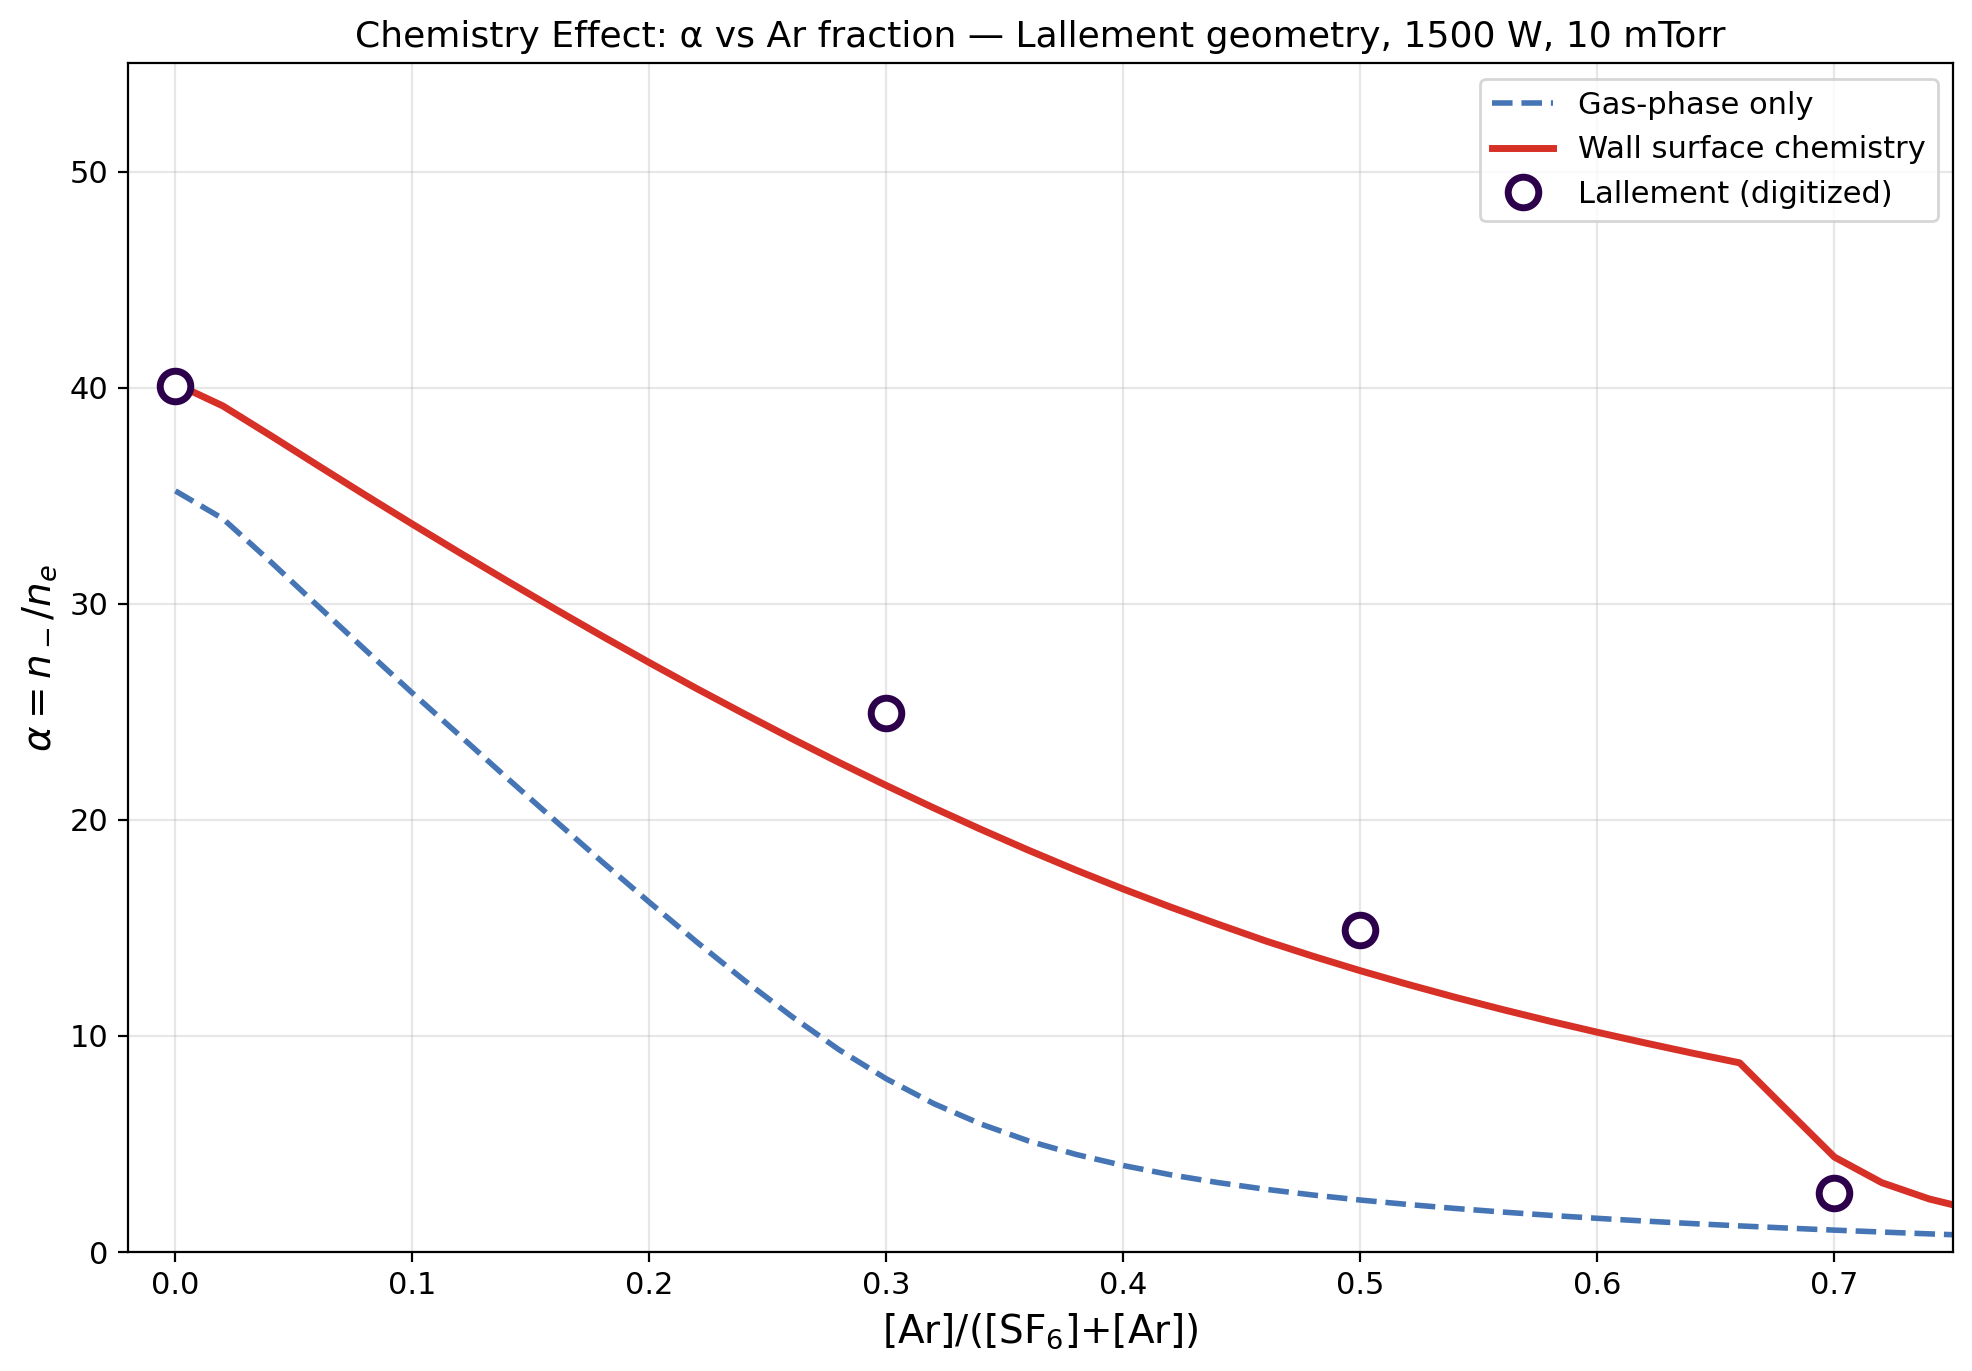
\includegraphics[width=0.9\textwidth]{fig1_alpha_chemistry_effect.png}
\caption{Electronegativity $\alpha$ vs Ar fraction at \SI{1500}{\watt}, \SI{10}{\milli\torr}: gas-phase model (dashed blue), wall surface chemistry extension (solid red), and digitized Lallement data (open circles).  The wall chemistry reduces the SSE by a factor of 26.}
\label{fig:wall_alpha_chem}
\end{figure}

\begin{table}[H]
\centering
\caption{Quantitative improvement from wall chemistry at \SI{1500}{\watt}, \SI{10}{\milli\torr}.}
\label{tab:wall_improvement}
\small
\begin{tabular}{lcccc}
\toprule
Ar fraction & Gas-phase $\alpha$ & Wall chem $\alpha$ & Lallement & Error reduction \\
\midrule
0\% & 35.2 & \textbf{40.2} & 40.1 & 12\% $\to$ 0.2\% \\
30\% & 8.0 & \textbf{21.6} & 24.9 & 68\% $\to$ 13\% \\
50\% & 2.4 & \textbf{13.0} & 14.9 & 84\% $\to$ 13\% \\
70\% & 1.0 & \textbf{4.4} & 2.7 & 62\% $\to$ 63\% \\
\bottomrule
\end{tabular}
\end{table}

\begin{figure}[H]
\centering
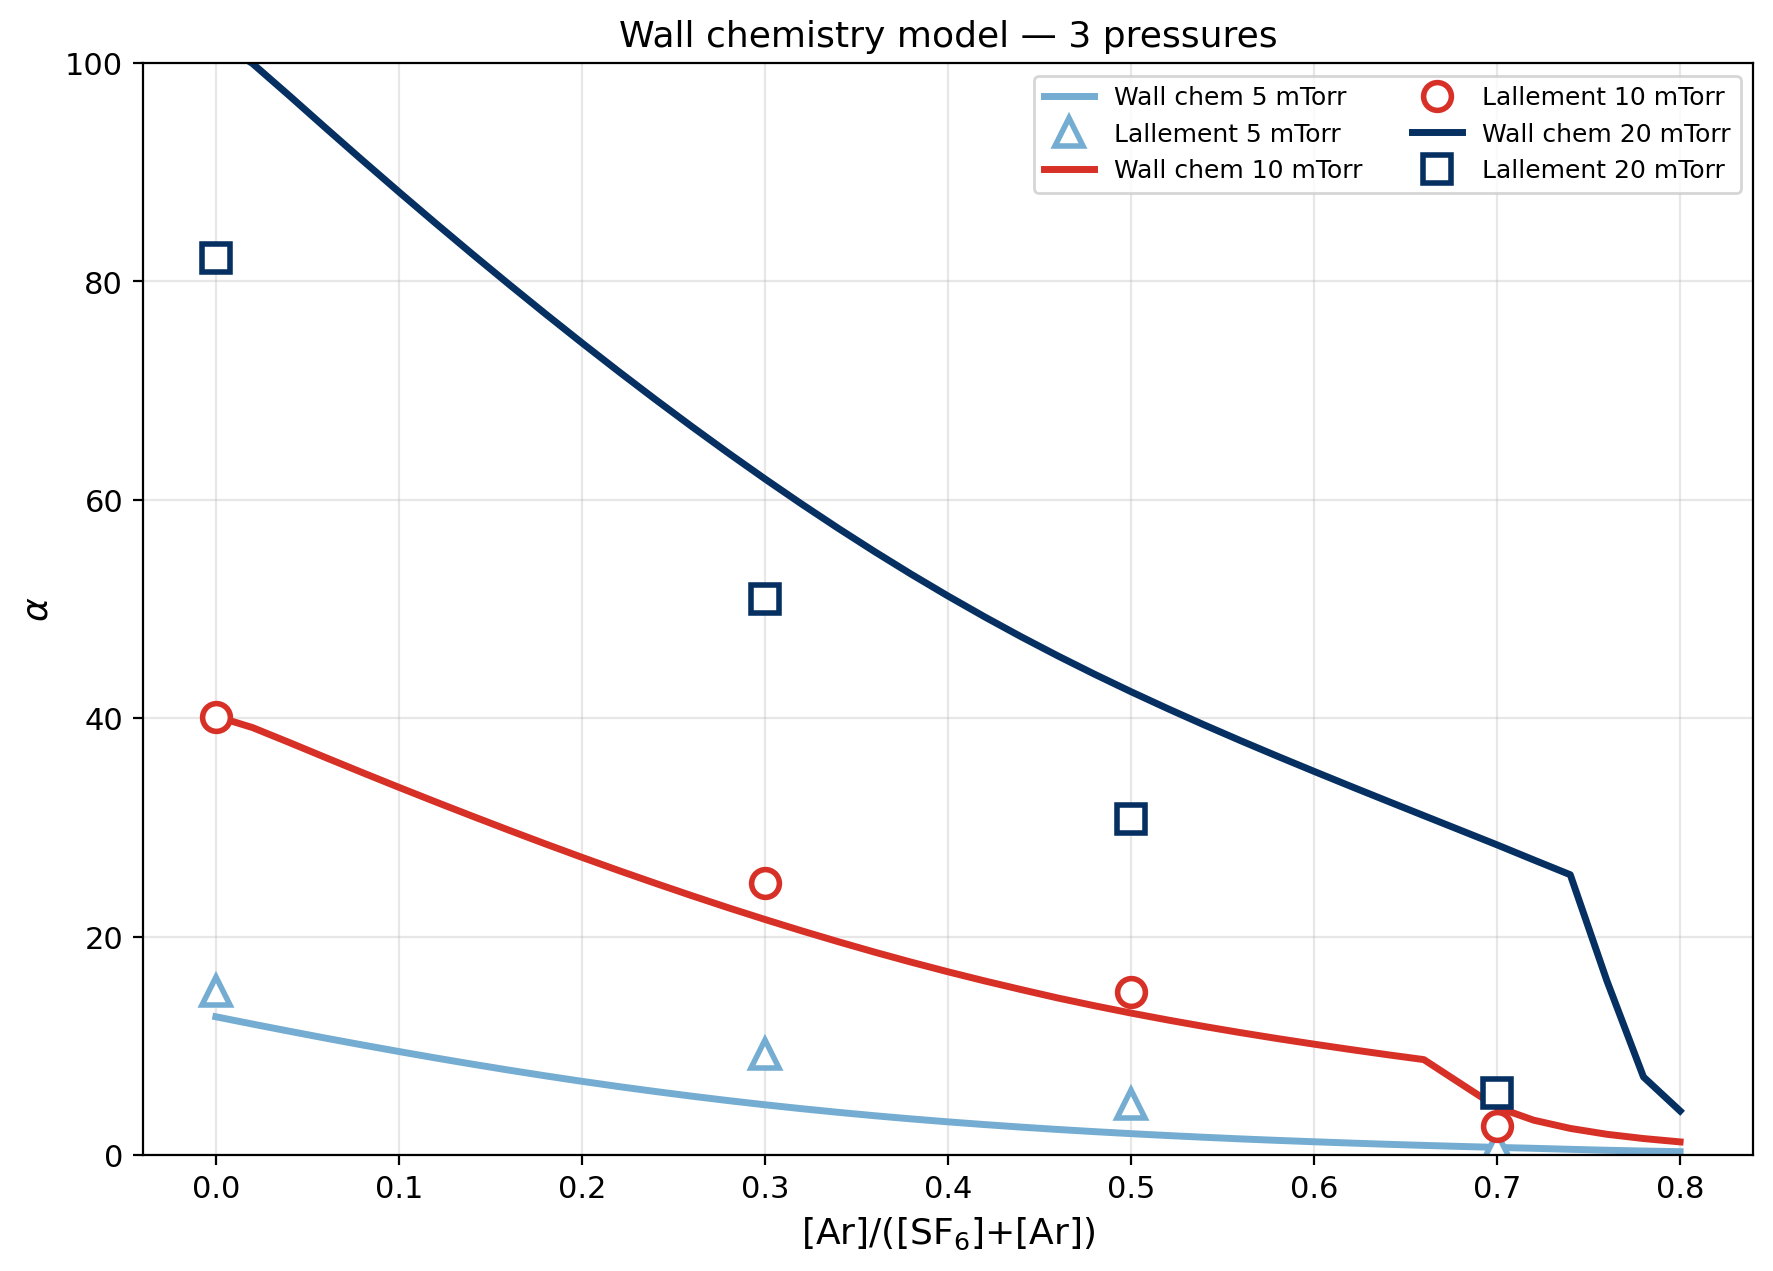
\includegraphics[width=0.9\textwidth]{fig2_alpha_3pressures.png}
\caption{Wall surface chemistry extension at 5, 10, and \SI{20}{\milli\torr} compared with digitized Lallement data.}
\label{fig:wall_alpha_3press}
\end{figure}

\begin{figure}[H]
\centering
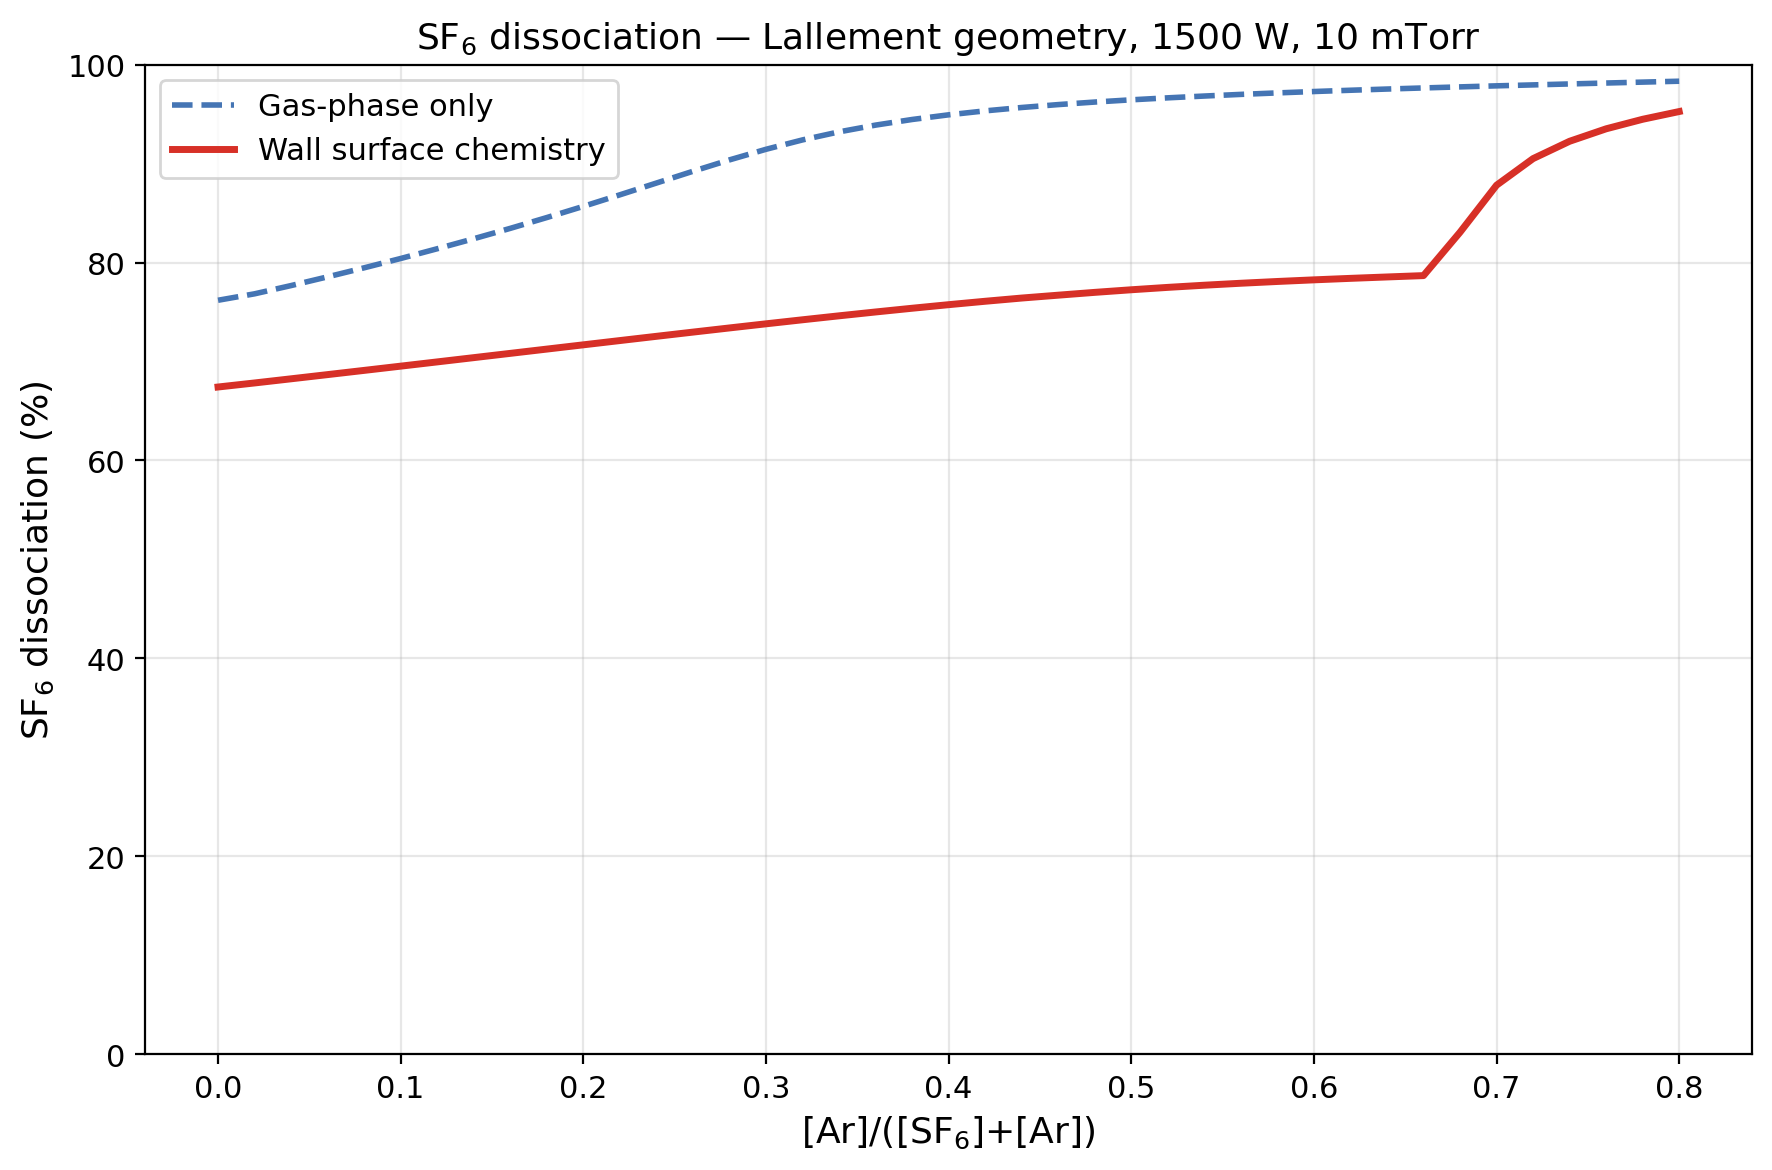
\includegraphics[width=0.8\textwidth]{fig3_dissociation_chemistry.png}
\caption{SF$_6$ dissociation fraction vs Ar dilution.  Wall surface chemistry buffers against the runaway dissociation that causes $\alpha$ to collapse in the gas-phase model.}
\label{fig:wall_dissociation}
\end{figure}

\begin{figure}[H]
\centering
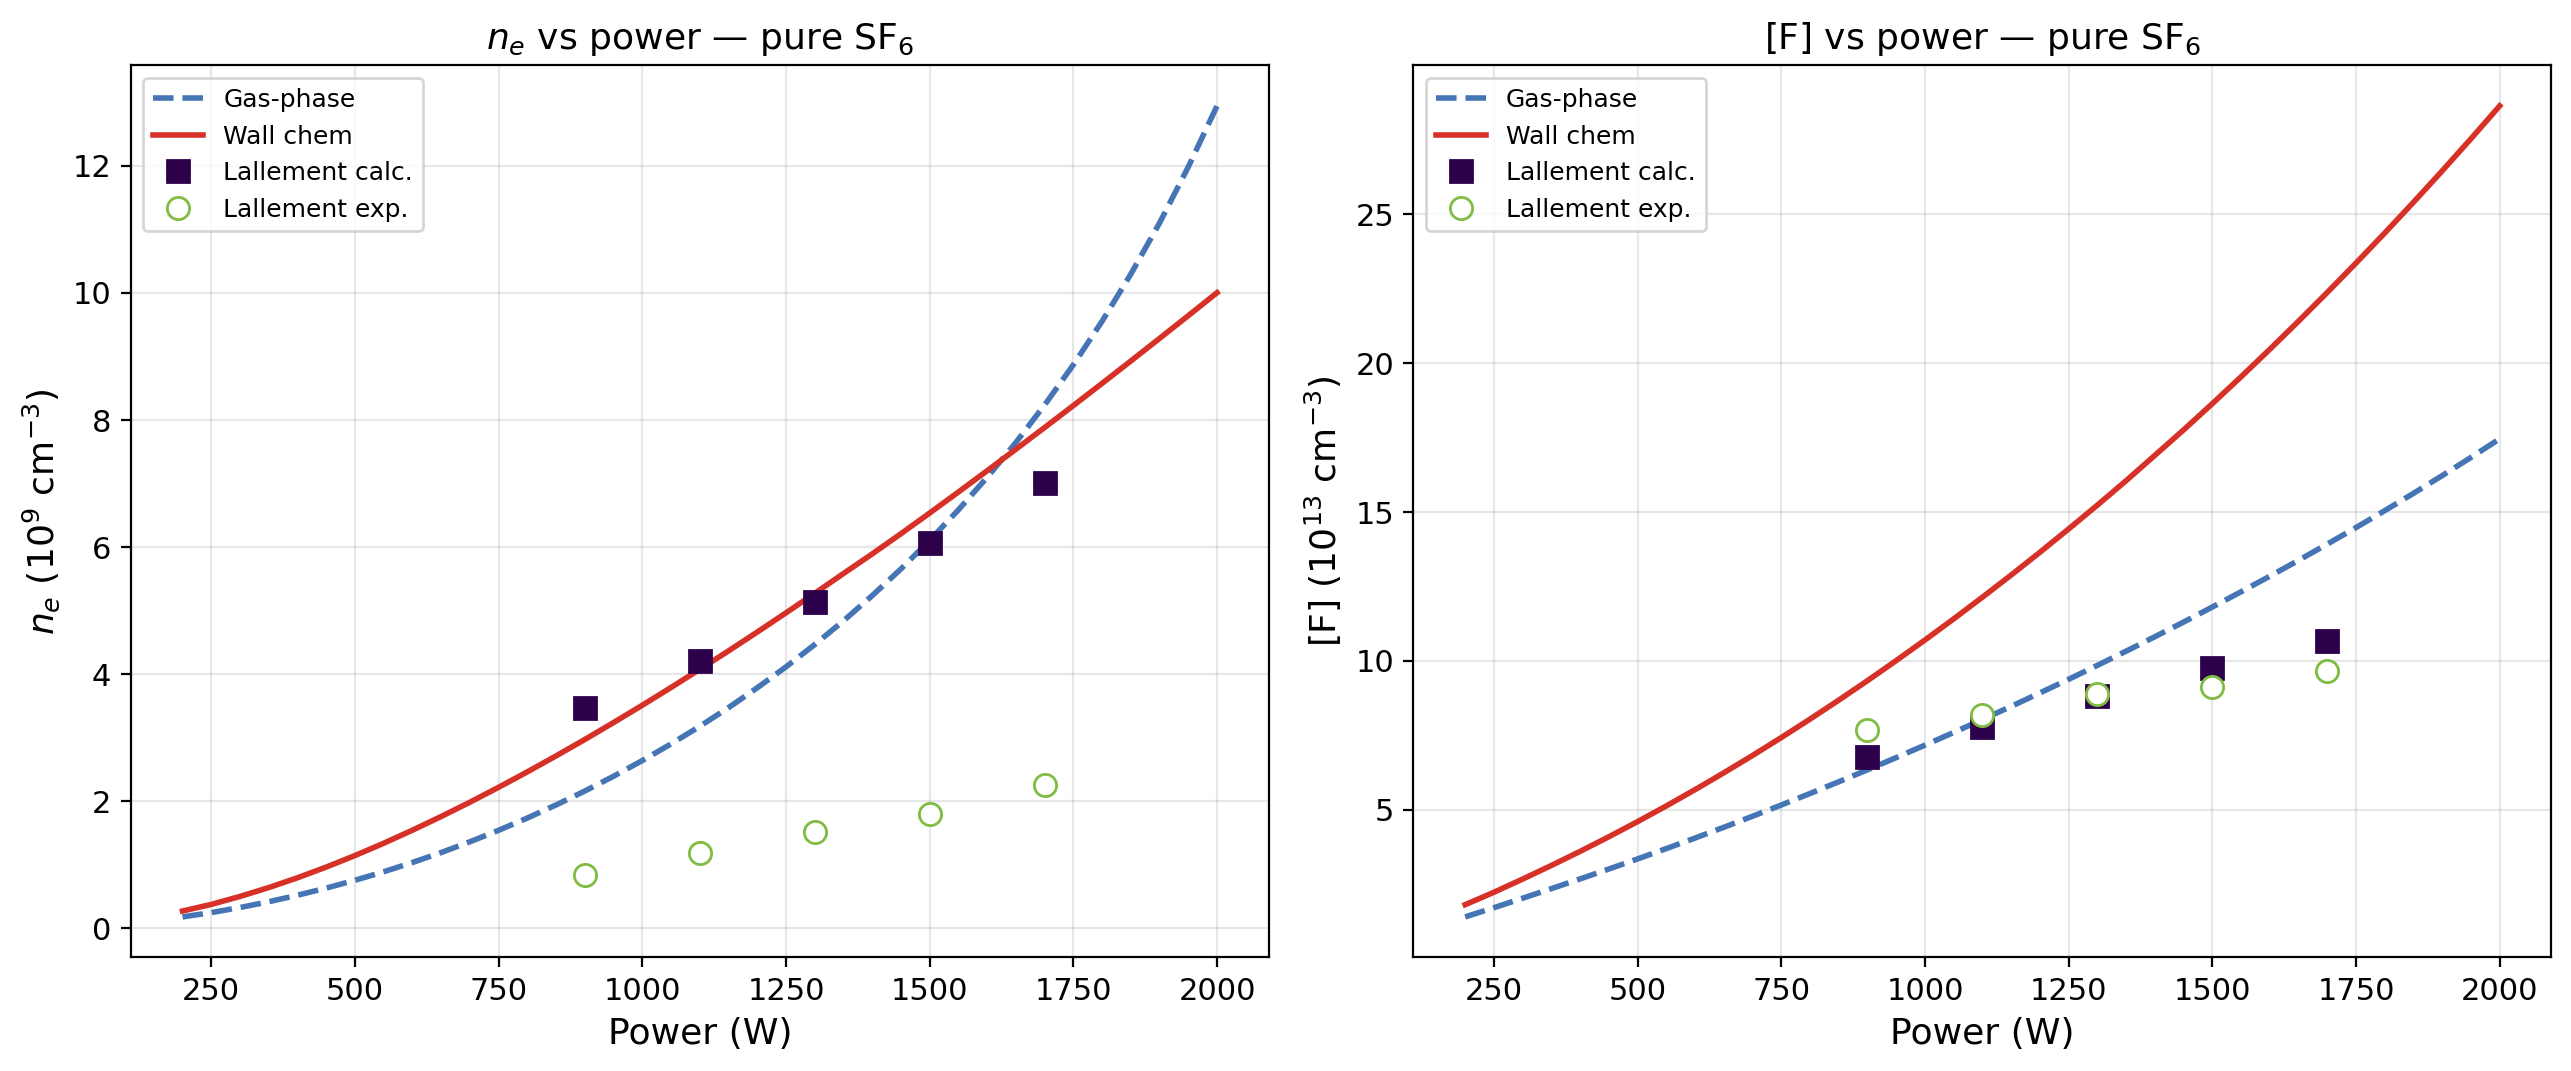
\includegraphics[width=\textwidth]{fig4_ne_F_vs_power.png}
\caption{Electron density $n_e$ and fluorine atom density [F] vs coupled power for pure SF$_6$ at \SI{10}{\milli\torr}, comparing both model variants with digitized Lallement data.}
\label{fig:wall_ne_F}
\end{figure}

%======================================================================
\section{Results: Geometry Effect}
\label{sec:wall_geom_results}
%======================================================================

\begin{figure}[H]
\centering
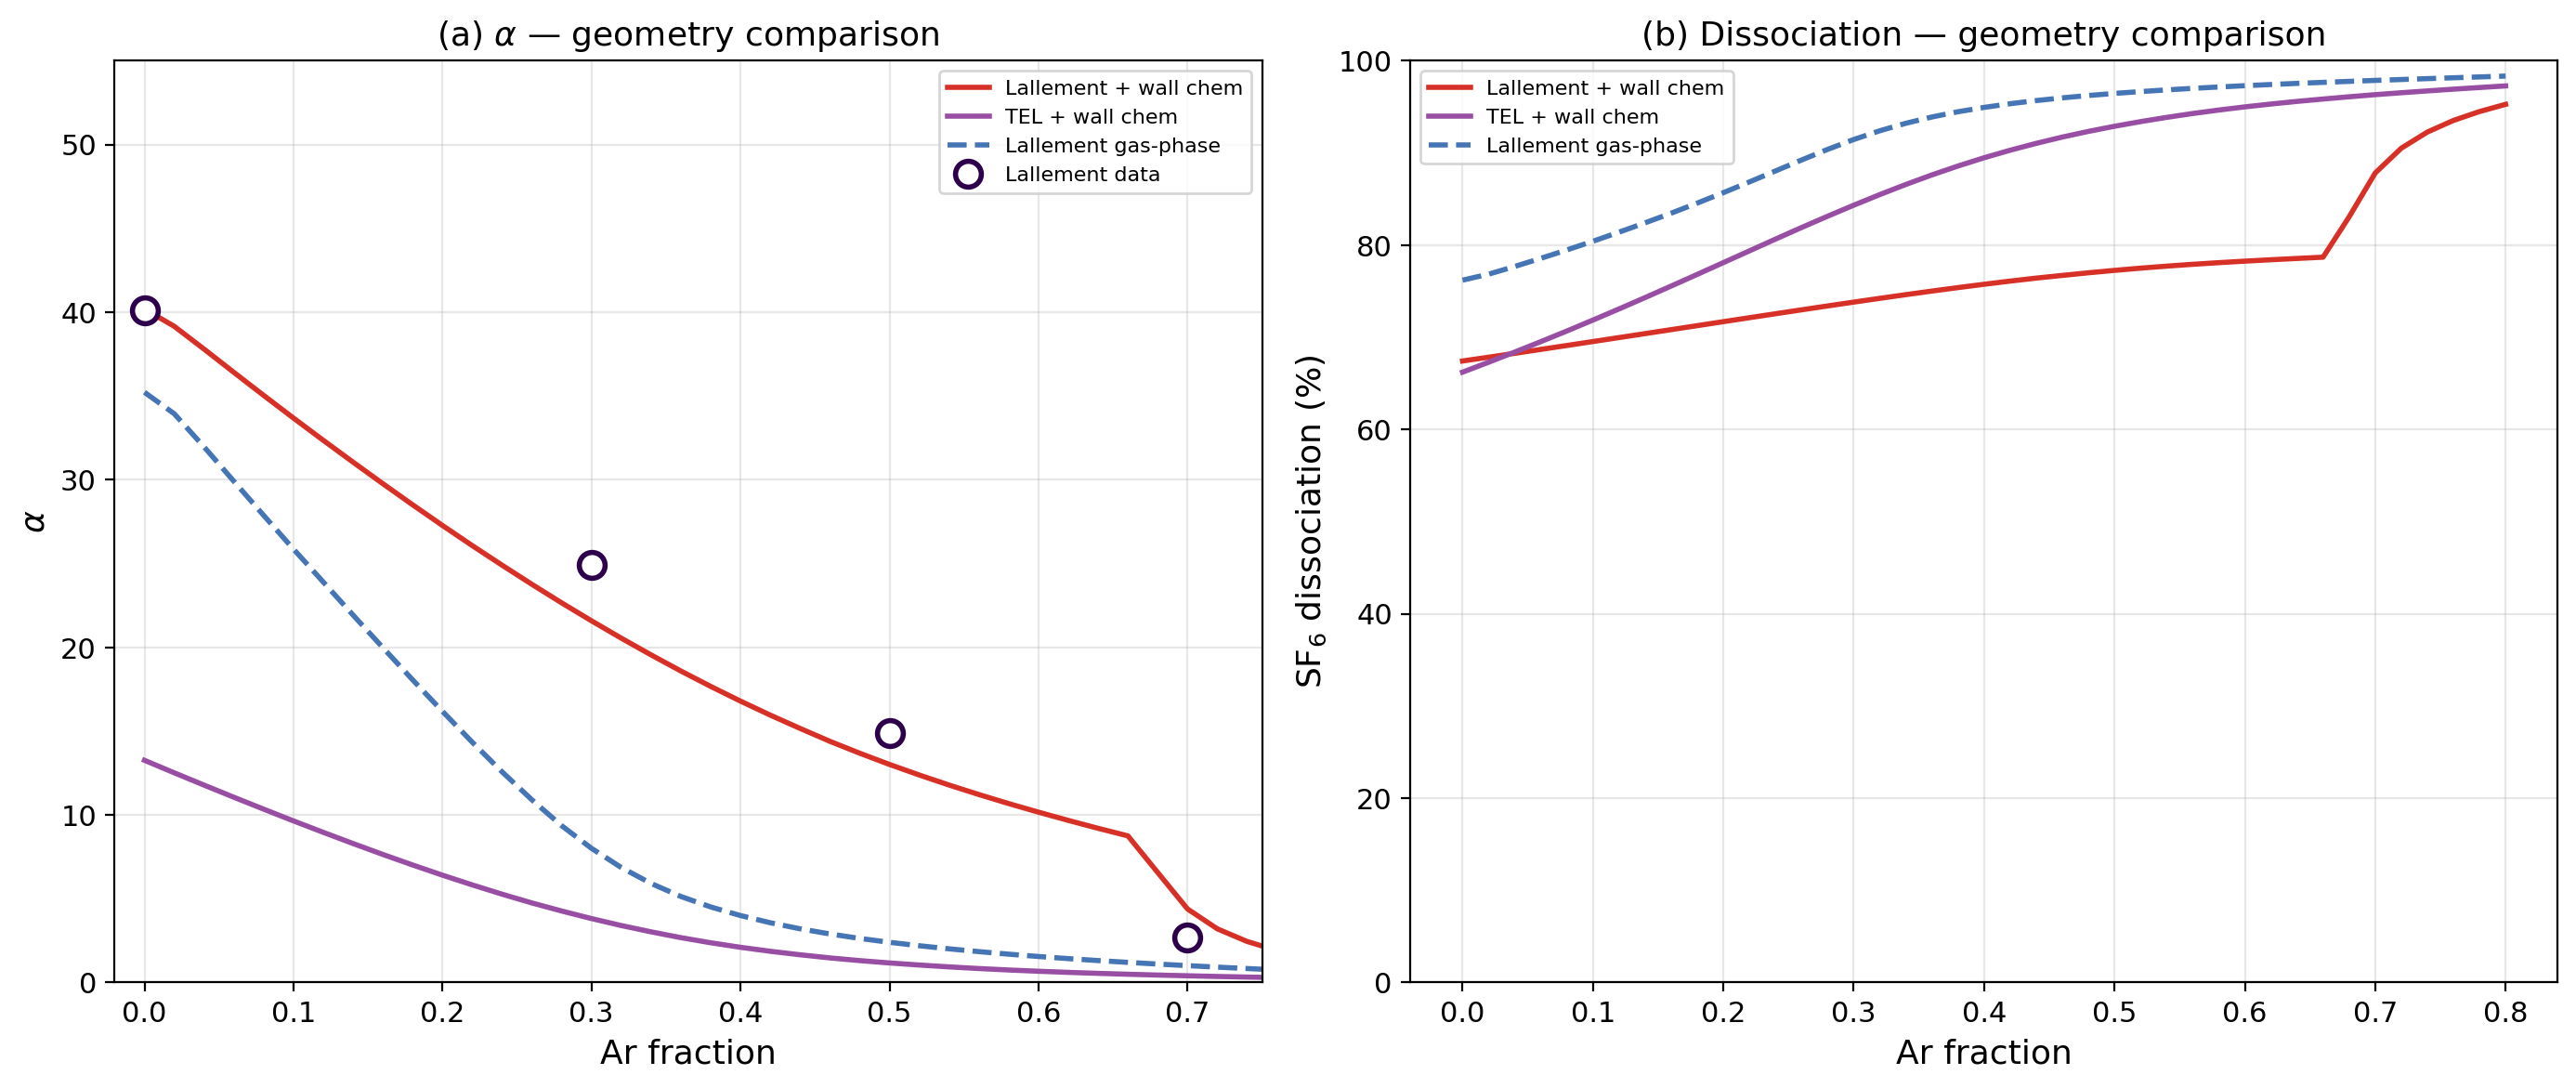
\includegraphics[width=\textwidth]{fig5_geometry_effect.png}
\caption{(a) Electronegativity $\alpha$ and (b) SF$_6$ dissociation fraction comparing Lallement and TEL geometries with wall surface chemistry.}
\label{fig:wall_geometry}
\end{figure}

At 30\% Ar with identical wall chemistry parameters: the Lallement geometry gives $\alpha = 21.6$ with 74\% dissociation, while the TEL geometry gives $\alpha = 3.8$ with 84\% dissociation.

\begin{figure}[H]
\centering
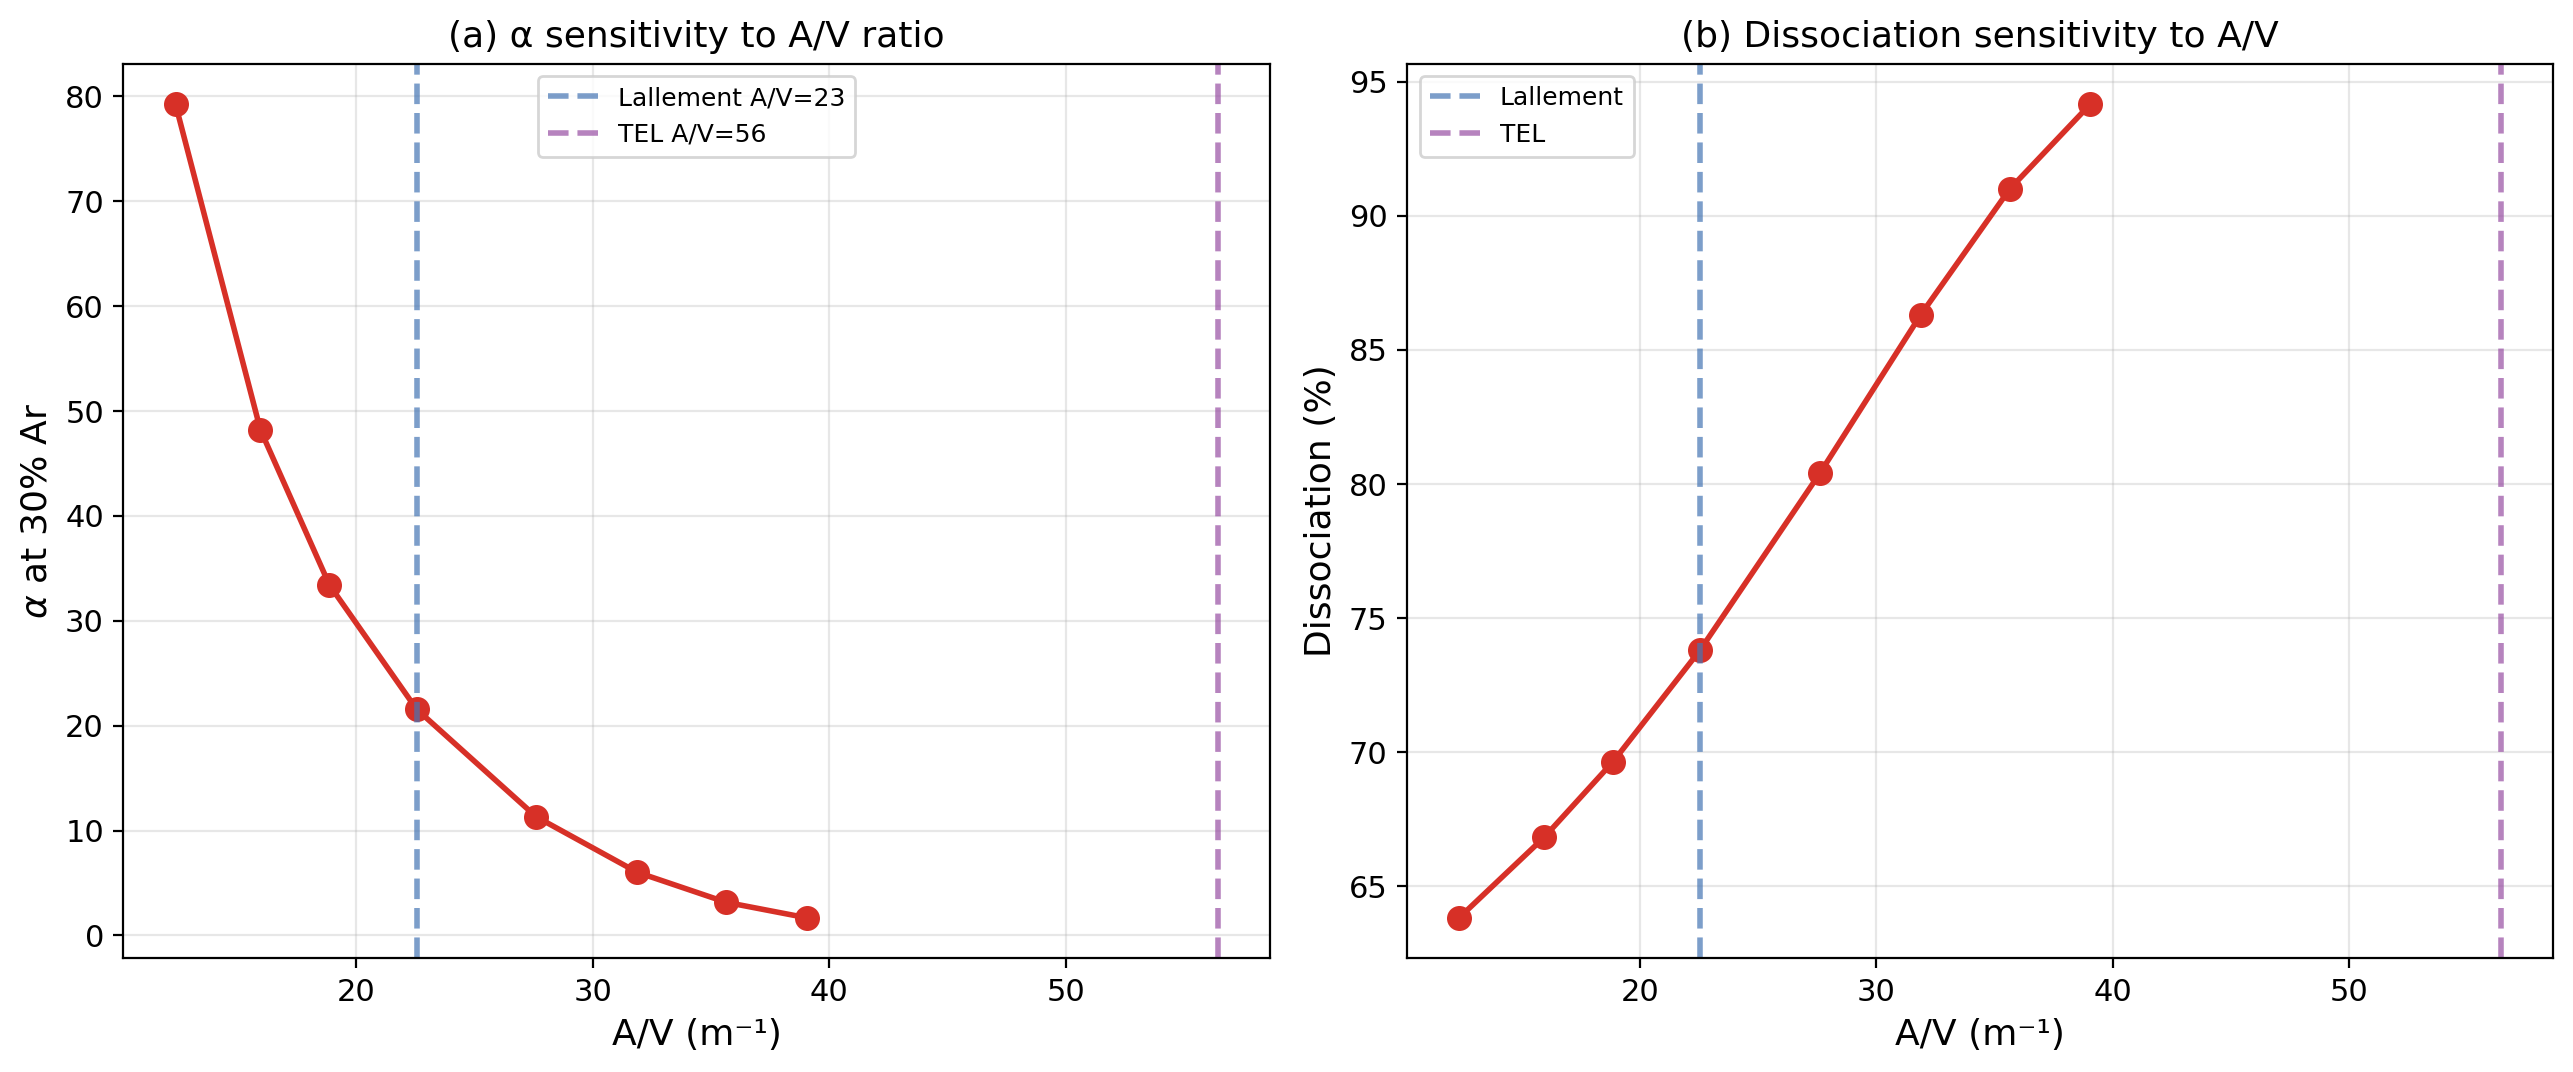
\includegraphics[width=\textwidth]{fig6_AV_sensitivity.png}
\caption{(a) $\alpha$ and (b) dissociation fraction at 30\% Ar as a function of reactor A/V ratio.  Higher A/V (smaller reactor) produces lower $\alpha$ because the electron density increase outweighs the additional wall area.}
\label{fig:wall_AV}
\end{figure}

%======================================================================
\section{TEL Benchmarking}
\label{sec:wall_tel}
%======================================================================

\subsection{Measurement Interpretation}
\label{sec:wall_tel_interp}

The following factors must be considered when comparing a zero-dimensional global model against spatially resolved TEL measurements~\cite{Mettler2025}:
\begin{itemize}[nosep]
\item \textbf{Actinometry} measures a line-averaged optical emission intensity ratio, not a local point measurement.
\item \textbf{Radical probe} measurements are local (${\sim}\SI{1}{\centi\meter}$ above wafer surface), and the ICP center density is approximately $10\times$ higher than the above-wafer density.
\item Radial density profiles show a decrease to ${\sim}25\%$ of the center value at the wafer edge.
\item Stage bias increases the measured [F] by a factor of 1.6--2.15.
\end{itemize}

\begin{figure}[H]
\centering
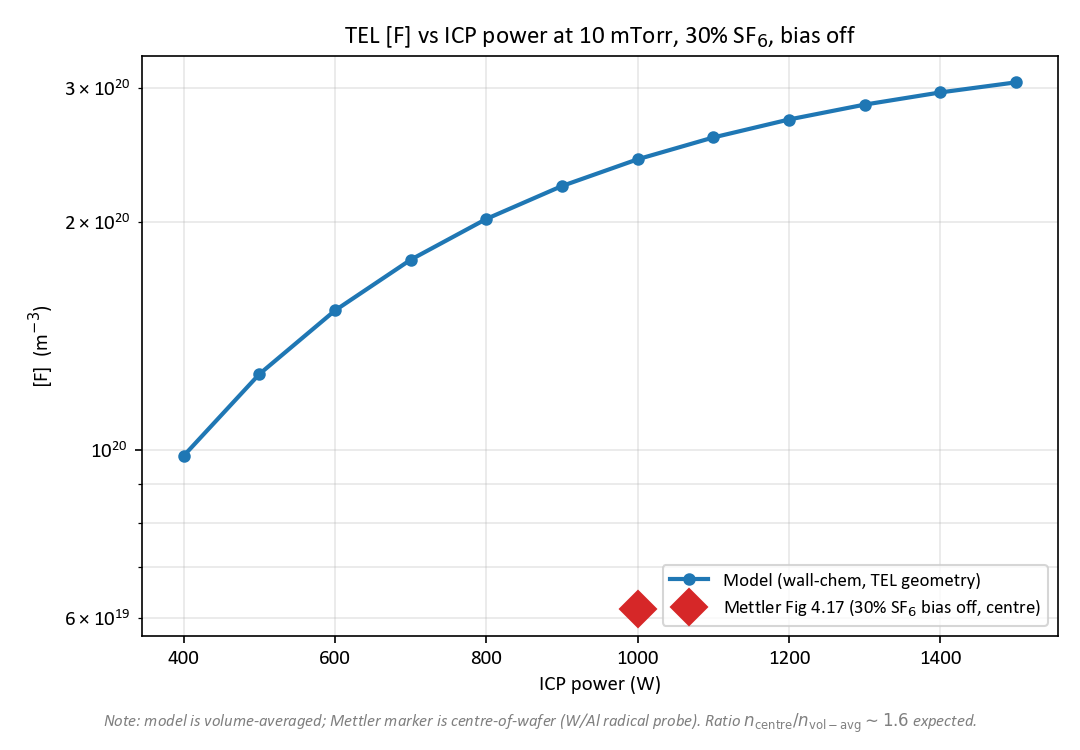
\includegraphics[width=0.85\textwidth]{tel_power_sweep_1000W_30pctAr.png}
\caption{TEL Case~1 (corrected): F radical density vs ICP power for the wall-chemistry-extended 0D model at Mettler's Fig~4.17 operating condition (\SI{10}{\milli\torr}, 30\% SF$_6$ / 70\% Ar, bias off), with the Mettler W/Al probe centre-of-wafer measurement at \SI{1000}{\watt} overlaid.  An earlier draft of this figure used \texttt{fig7\_tel\_F\_vs\_power.png} with a ``\SI{50}{\milli\torr}, 50\% Ar'' caption that corresponded to Mettler's PMIC helicon Fig~4.5; that figure has been withdrawn as it is not a TEL benchmark.}
\label{fig:wall_tel_power}
\end{figure}

\begin{figure}[H]
\centering
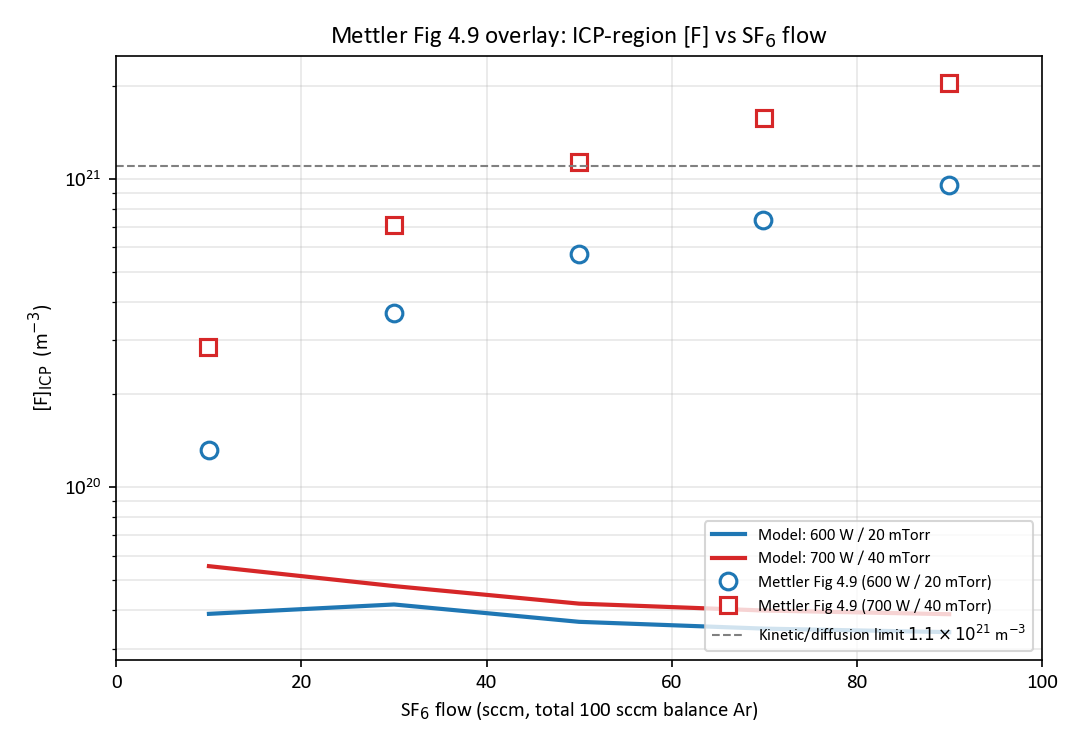
\includegraphics[width=0.85\textwidth]{mettler_fig49_overlay.png}
\caption{TEL Case~2: [F]$_{\mathrm{ICP}}$ vs SF$_6$ flow at Mettler Fig~4.9~\cite{Mettler2025} two operating branches.  Low-$p$ branch: \SI{600}{\watt} / \SI{20}{\milli\torr}; high-$p$ branch: \SI{700}{\watt} / \SI{40}{\milli\torr}.  Mettler measured $[F]_{\mathrm{ICP}} \approx 1.0\times10^{21}$\,m$^{-3}$ at 90 sccm SF$_6$ in the low-$p$ branch and $2.0\times10^{21}$\,m$^{-3}$ in the high-$p$ branch.  The dashed line marks the kinetic-to-diffusion-limited threshold at $1.1\times10^{21}$\,m$^{-3}$ (Mettler Table~4.4): all model predictions lie safely below this in the kinetic regime.}
\label{fig:wall_tel_flow}
\end{figure}

\begin{figure}[H]
\centering
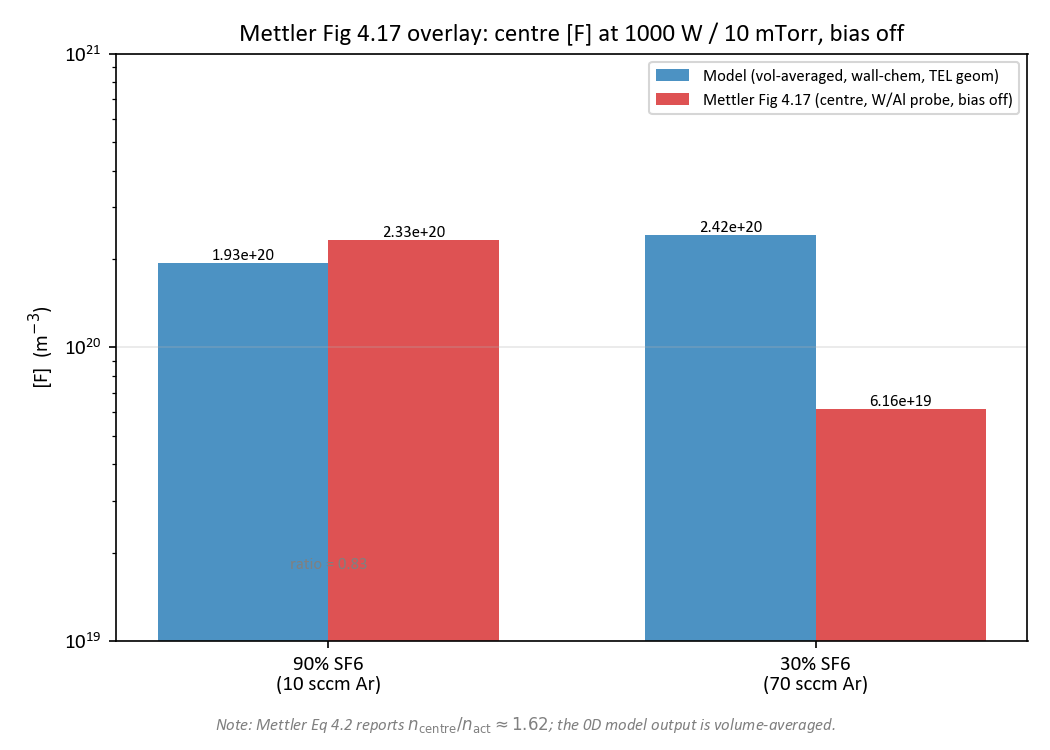
\includegraphics[width=0.80\textwidth]{mettler_fig417_overlay.png}
\caption{TEL Case~3: centre-of-wafer [F] at Mettler Fig~4.17~\cite{Mettler2025} condition (\SI{1000}{\watt} / \SI{10}{\milli\torr} / \SI{100}{sccm}~total, bias off) for two compositions.  Mettler's centre-to-edge drop is \textbf{76\%} at 90:10 SF$_6$:Ar and \textbf{67\%} at 30:70 SF$_6$:Ar---a 67\%--76\% range across this figure alone.  The ``74\%'' number sometimes used in the literature is \emph{not} from Fig~4.17 bias-off; it refers specifically to the Fig~4.14 cubic fit at 70:30 SF$_6$:Ar with \SI{200}{\watt} bias on.  Our $\gamma_{\mathrm{Al}} = 0.18$ wall-chemistry calibration (Section~\ref{sec:wall_intro}) was tuned against the 90\%-SF$_6$ branch; the factor-of-$\sim$4 overprediction at 30\%-SF$_6$ quantifies the composition-dependence gap that motivates the deferred composition sweep in Chapter~\ref{ch:future}.}
\label{fig:wall_tel_center}
\end{figure}

%======================================================================
\section{Discussion}
\label{sec:wall_discussion}
%======================================================================

\paragraph{Wall surface chemistry resolves the dominant structural error.}  The gas-phase model's $\alpha$ collapses at $>30\%$ Ar because the Troe-corrected neutral recombination rates at \SI{10}{\milli\torr} are too slow to rebuild SF$_6$ from dissociation fragments.  Wall-mediated fluorination provides the missing regeneration pathway, buffering SF$_6$ against the runaway depletion feedback loop.  The $26\times$ reduction in SSE confirms that wall chemistry addresses the physics that was missing.

\paragraph{Geometry modulates the magnitude of the wall chemistry effect.}  Despite the TEL's $2.5\times$ higher A/V ratio, the net wall chemistry effect is weaker because: the TEL volume is $10\times$ smaller, producing $15\times$ higher $n_e$; the TEL residence time is $24\times$ shorter; and dissociation scales with $n_e$ (power density dependent), while wall production scales linearly with A/V.

\paragraph{TEL benchmarking as a transferability assessment.}  The remaining discrepancies reflect the combined influence of: (i) unknown power coupling efficiency $\eta_\mathrm{TEL}$, (ii) the two-region ICP/wafer architecture, (iii) fundamentally different measurement techniques, and (iv) wall chemistry probabilities calibrated for Lallement wall materials.

%======================================================================
\section{Summary}
\label{sec:wall_summary}
%======================================================================

\begin{enumerate}[nosep]
\item Wall surface chemistry reduces the $\alpha$ SSE by a factor of 26, resolving the dominant structural error.
\item Only 0.7\% of the Kokkoris et al.~\cite{Kokkoris2009} surface reaction probabilities are required for the stainless-steel Lallement reactor.
\item The geometry comparison demonstrates that wall chemistry corrects the dissociation physics, while reactor geometry modulates the magnitude of the correction.
\item For compact, high-power-density reactors such as the TEL etcher, reactor-specific recalibration of surface parameters is needed.
\item Remaining discrepancies motivate future work on spatially resolved models.
\end{enumerate}

With the wall chemistry model established as the adopted baseline, the next chapter investigates a prominent feature of this model: the stiff $\alpha$ transition at ${\sim}67\%$ Ar.  This transition, absent in the gas-phase model, reveals the limits of wall chemistry buffering and provides insight into the nonlinear coupling between surface and gas-phase processes.


%=============================================================================
\chapter{Electronegativity Transition and Root-Cause Analysis}
\label{ch:kink}
%=============================================================================

This chapter merges the phenomenological characterization of the stiff electronegativity transition (``kink'') at ${\sim}67\%$ Ar with the root-cause parameter identification, providing a unified treatment of the wall chemistry buffer exhaustion mechanism.

%======================================================================
\section{Problem Statement}
\label{sec:kink_problem}
%======================================================================

The wall surface chemistry extension of Chapter~\ref{ch:wallchem} exhibits a stiff transition in the electronegativity parameter $\alpha = n_-/n_e$ at approximately 67\% Ar.  Between 66\% and 69\% Ar, $\alpha$ drops from 8.7 to 5.3---a factor of 1.6 over a 3 percentage-point interval---whereas at Ar fractions below 66\%, $\alpha$ decreases smoothly at a rate of $d\alpha/d(\mathrm{Ar\%}) \approx -0.23$ per percentage point.  The gas-phase-only model does not exhibit this feature; its $\alpha$ curve is smooth and monotonic throughout.  The transition occurs well within the strongly electronegative regime ($\alpha \gg 1$), distinguishing it from the classical EN$\to$EP mode transition at $\alpha \approx 1$ analyzed by Lieberman and Lichtenberg~\cite{Lieberman2005}.

%======================================================================
\section{Phenomenology}
\label{sec:kink_phenom}
%======================================================================

\begin{figure}[H]
\centering
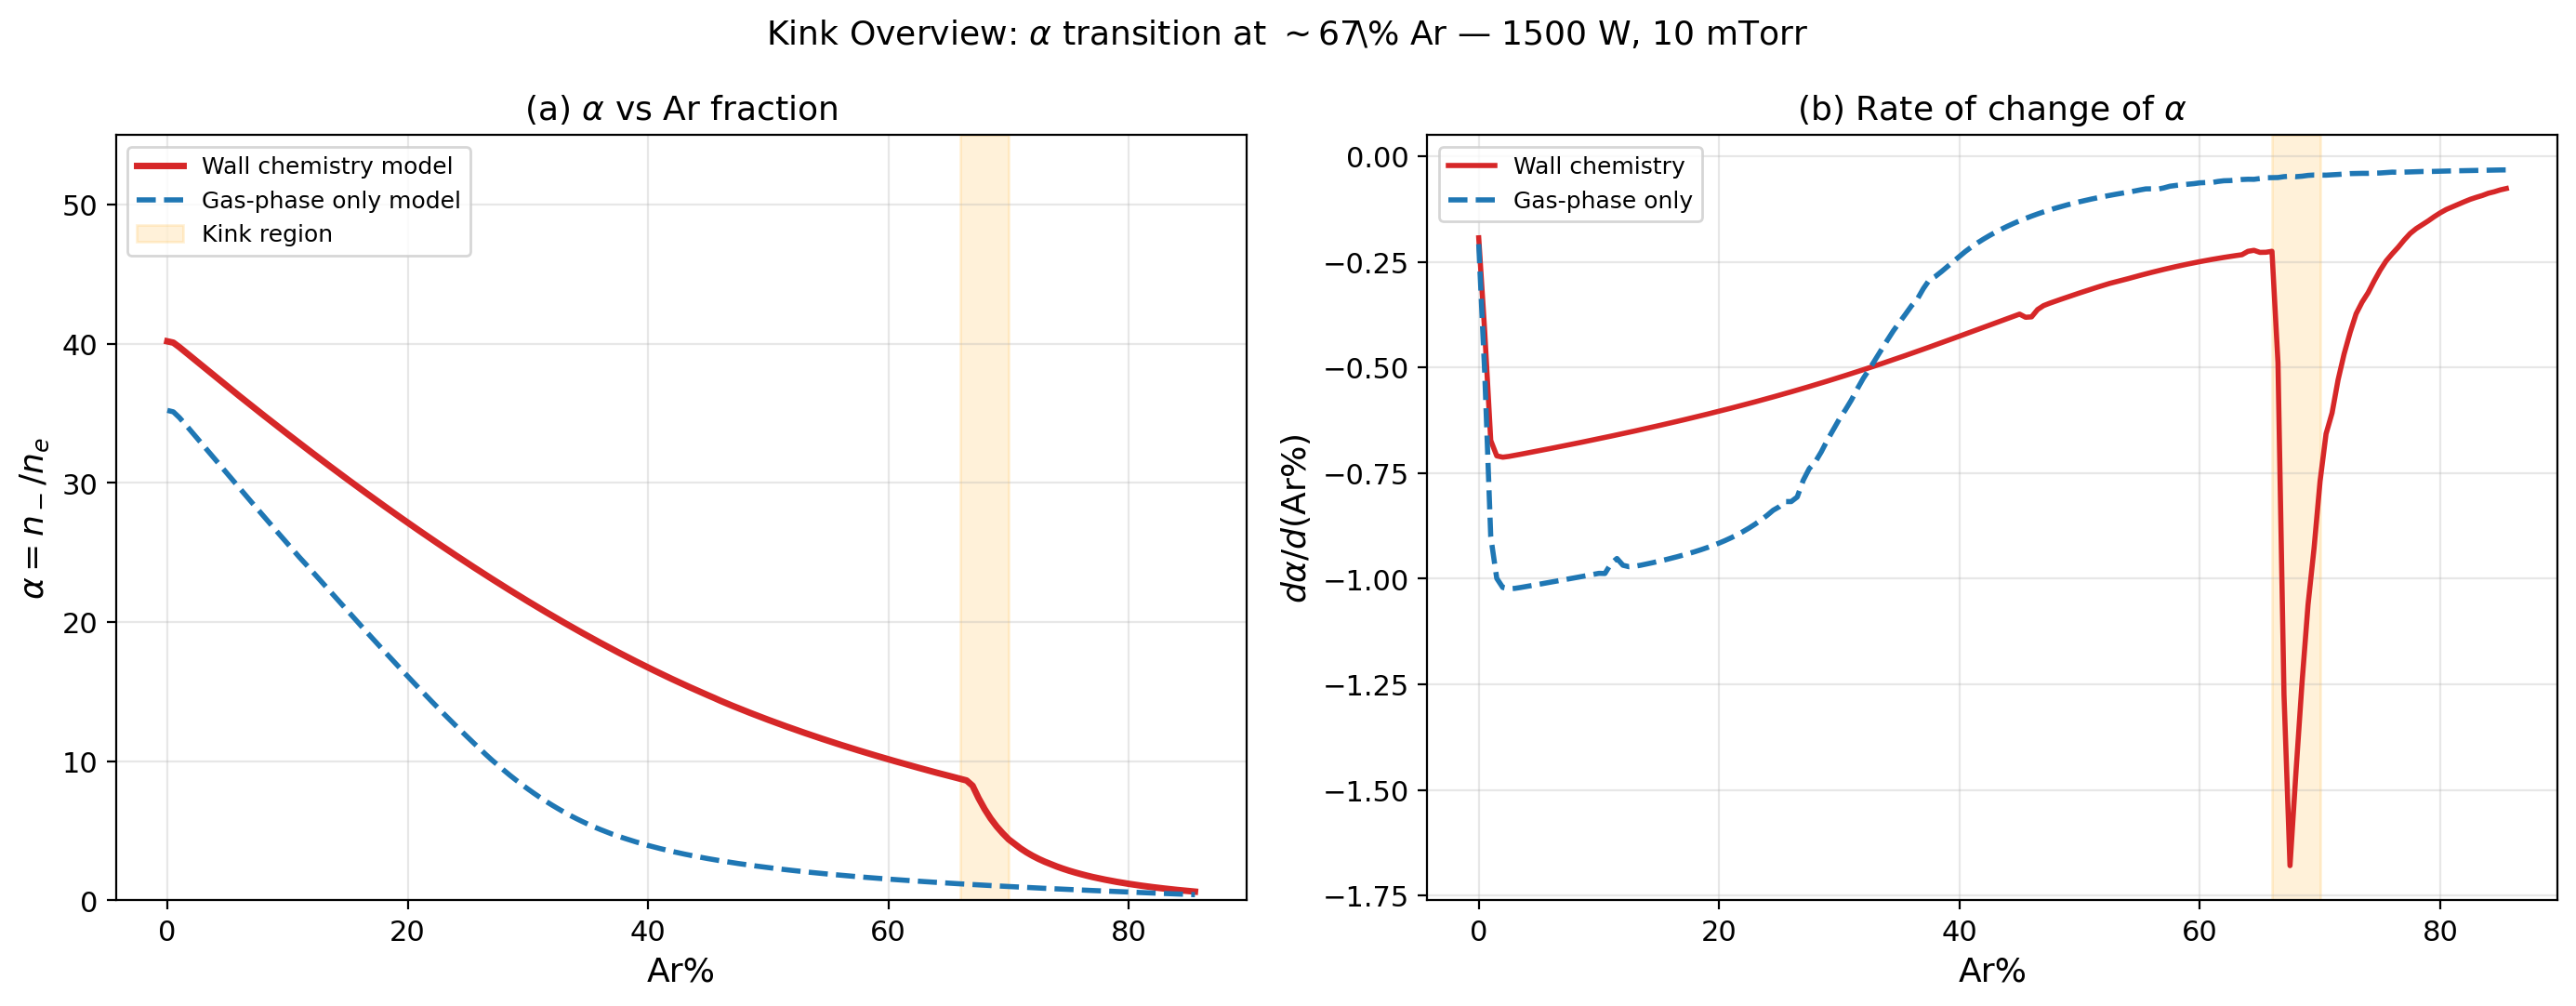
\includegraphics[width=\textwidth]{fig1_kink_overview.png}
\caption{(a)~$\alpha$ vs Ar fraction for the wall chemistry (red) and gas-phase (blue) models.  The kink region (orange band) is visible between 66--69\% Ar.  (b)~Rate of change $d\alpha/d(\mathrm{Ar\%})$: the wall chemistry curve shows a sharp dip from $-0.23$ to $-1.8$ at 67.5\% Ar.}
\label{fig:kink_overview}
\end{figure}

\begin{table}[H]
\centering
\caption{Plasma parameters through the kink region at \SI{1500}{\watt}, \SI{10}{\milli\torr}.}
\label{tab:kink_params}
\begin{tabular}{lcccccc}
\toprule
\textbf{Ar\%} & $\alpha$ & $n_e$ (cm$^{-3}$) & $\Te$ (eV) & SF$_6$\% & [F] (cm$^{-3}$) & $d\alpha/d$\% \\
\midrule
65 & 8.97 & $3.00\times10^{10}$ & 2.222 & 21.4\% & $6.18\times10^{14}$ & $-0.23$ \\
66 & 8.74 & $3.06\times10^{10}$ & 2.211 & 21.3\% & $6.34\times10^{14}$ & $-0.23$ \\
\textcolor{red}{\textbf{67}} & \textcolor{red}{\textbf{8.24}} & $3.23\times10^{10}$ & 2.197 & 20.5\% & $6.37\times10^{14}$ & \textcolor{red}{\textbf{$-0.75$}} \\
\textcolor{red}{\textbf{68}} & \textcolor{red}{\textbf{6.56}} & $4.00\times10^{10}$ & 2.160 & 16.9\% & $6.18\times10^{14}$ & \textcolor{red}{\textbf{$-1.68$}} \\
69 & 5.32 & $4.84\times10^{10}$ & 2.129 & 14.2\% & $5.99\times10^{14}$ & $-1.25$ \\
70 & 4.39 & $5.72\times10^{10}$ & 2.102 & 12.2\% & $5.79\times10^{14}$ & $-0.93$ \\
72 & 3.20 & $7.38\times10^{10}$ & 2.068 & 9.5\% & $5.41\times10^{14}$ & $-0.50$ \\
75 & 2.14 & $1.06\times10^{11}$ & 2.028 & 6.5\% & $4.64\times10^{14}$ & $-0.28$ \\
\bottomrule
\end{tabular}
\end{table}

%======================================================================
\section{Context: EN$\to$EP Transitions in Electronegative Discharges}
\label{sec:kink_context}
%======================================================================

\subsection{Theoretical Framework: Multiple Solution Branches}
\label{sec:kink_theory}

Lichtenberg et al.~\cite{Lichtenberg1997} showed analytically that the coupled particle and power balances in electronegative global models admit multiple solution branches.  The steady-state particle balance produces a cubic equation in $n_e$ whose roots correspond to a high-$\alpha$ (EN) branch, a low-$\alpha$ (EP) branch, and an unstable intermediate branch.  As the absorbed power increases past a critical value $P_c$, the EN branch ceases to exist and the system must jump to the EP branch.  Lieberman and Lichtenberg~\cite{Lieberman2005} generalized this to include the effect of negative-ion spatial profiles.

\subsection{Bifurcation in Ar/SF$_6$ ICP Discharges}
\label{sec:kink_bifurcation}

Lichtenberg et al.~\cite{Lichtenberg2012} investigated the EN$\to$EP transition specifically in Ar/SF$_6$ ICP discharges, observing experimentally that large-amplitude relaxation oscillations arise from a Hopf bifurcation at the EN--EP boundary.  The instability window becomes narrower as the argon partial pressure increases, making the jump sharper.  The kink in the present model can be understood as the steady-state projection of this same bifurcation structure.

\subsection{Oxygen Discharges: Wall Recombination Controls the Transition}
\label{sec:kink_oxygen}

Gudmundsson et al.~\cite{Gudmundsson2001} showed that in O$_2$ ICP plasmas, the electronegativity depends sensitively on the wall recombination coefficient $\gamma_\mathrm{O}$ of atomic oxygen.  Changing wall material altered $\alpha$ by up to $3\times$ at the same power and pressure.  Gudmundsson~\cite{Gudmundsson2002} further showed that the EN$\to$EP transition manifests as a near-discontinuous jump in $\alpha$ when the absorbed power exceeds a critical value, with the wall recombination probability of atomic fluorine as the most sensitive parameter.

\subsection{O$_2$/Ar Mixtures: Composition-Driven Dissociation Enhancement}
\label{sec:kink_O2Ar}

Gudmundsson and Thorsteinsson~\cite{Gudmundsson2007} studied O$_2$/Ar mixtures and showed that increasing the Ar fraction produces three coupled effects: rising $n_e$ from cheaper Ar ionization, increased O$_2$ dissociation, and dropping electronegativity.  The parallel to the SF$_6$/Ar system is direct.

\subsection{Experimental Observations in SF$_6$/Ar}
\label{sec:kink_expt}

Chabert et al.~\cite{Chabert1999} measured $\alpha$ in SF$_6$/Ar ICP discharges and observed that $\alpha$ decreases rapidly with both power and Ar fraction.  The transition appears as a steep but continuous decline, consistent with the present model.  Tuszewski and White~\cite{Tuszewski2002} reported $\Te = 2.6$--\SI{3.2}{\electronvolt} in the EN regime, consistent with the model's $\Te = \SI{2.2}{\electronvolt}$ at the kink location.

\subsection{Relationship to the Present Kink}
\label{sec:kink_comparison}

\begin{table}[H]
\centering\small
\caption{Comparison of the classical EN$\to$EP transition with the wall chemistry kink.}
\label{tab:kink_comparison}
\begin{tabular}{lcc}
\toprule
\textbf{Feature} & \textbf{Classical EN$\to$EP} & \textbf{Present kink} \\
\midrule
$\alpha$ at transition & $\sim$1 & $\sim$8 \\
Control parameter & Power & Composition (Ar fraction) \\
Mechanism & Ionization exceeds attachment & Wall buffer exhaustion \\
Wall chemistry role & Shifts threshold location & \textit{Is} the buffer that fails \\
Transition width & 50--\SI{200}{\watt} or $\sim$10\% Ar & $\sim$3\% Ar (67--70\%) \\
Post-transition state & $\alpha \ll 1$ (EP) & $\alpha \approx 2$--4 (weakly EN) \\
Observed in & O$_2$, Cl$_2$, SF$_6$ (theory + expt.) & SF$_6$/Ar with wall chem.\ (this work) \\
\bottomrule
\end{tabular}
\end{table}

%======================================================================
\section{Root Cause: Wall Chemistry Buffer Exhaustion}
\label{sec:kink_rootcause}
%======================================================================

\subsection{The Buffering Mechanism}
\label{sec:kink_buffer}

Below 66\% Ar, the wall surface chemistry provides a buffer against SF$_6$ depletion through two channels:

\begin{enumerate}[leftmargin=*,nosep]
\item \textbf{Sequential fluorination:} F + SF$_5$(wall) $\to$ SF$_6$(gas), returning SF$_6$ at rate $R_\mathrm{wall} = p_\mathrm{fluor} \cdot \theta_{\mathrm{SF}_5} \cdot \Gamma_\mathrm{F} \cdot A/V$
\item \textbf{Eley--Rideal recombination:} SF$_5$ + F(wall) $\to$ SF$_6$(gas), at rate $p_\mathrm{wr} \cdot \theta_\mathrm{F} \cdot \Gamma_{\mathrm{SF}_5} \cdot A/V$
\end{enumerate}

A threshold Ar fraction exists at which the wall regeneration rate becomes insufficient to maintain the SF$_6$ reservoir against the electron-driven dissociation rate.

\subsection{Quantitative Rate Analysis}
\label{sec:kink_rates}

\begin{figure}[H]
\centering
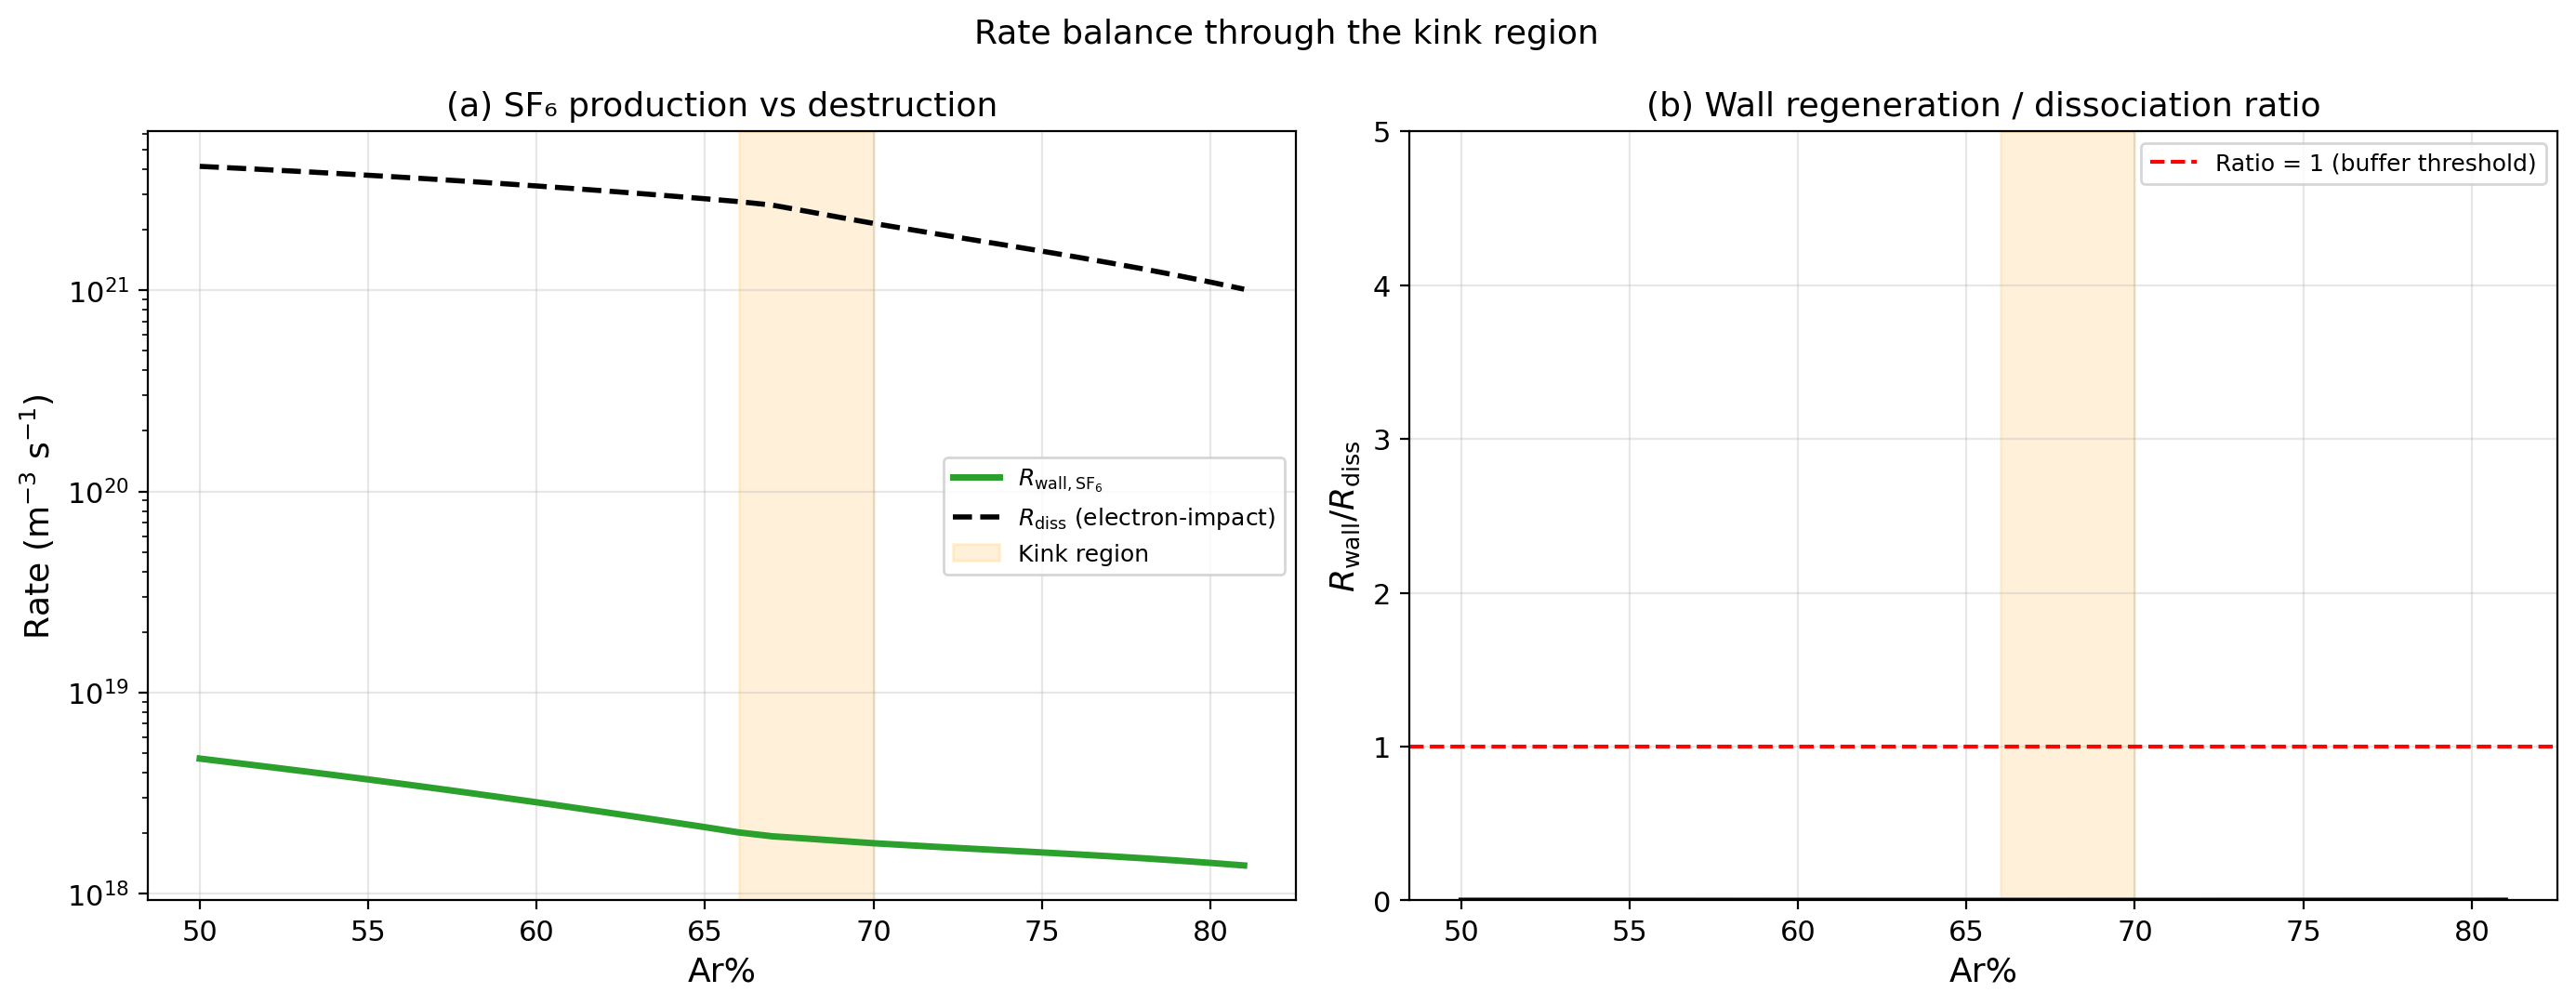
\includegraphics[width=\textwidth]{fig4_rate_balance.png}
\caption{(a)~SF$_6$ production (wall + Troe) and destruction (electron-impact dissociation) rates.  (b)~Ratio of wall regeneration to dissociation rate.  The kink region corresponds to where dissociation growth outpaces wall regeneration.}
\label{fig:kink_rate_balance}
\end{figure}

\subsection{Why the Gas-Phase Model Does Not Show a Kink}
\label{sec:kink_gasphase}

The gas-phase model does not exhibit the kink because it has already lost the buffering battle at much lower Ar fractions.  Without wall chemistry, the gas-phase Troe recombination at \SI{10}{\milli\torr} is too slow to buffer dissociation at any Ar fraction above ${\sim}20\%$.

%======================================================================
\section{Mechanism: Positive Feedback Threshold Crossing}
\label{sec:kink_feedback}
%======================================================================

The kink is a threshold-crossing phenomenon in a coupled nonlinear system.  The governing feedback loop is:
\begin{equation}
\underbrace{\text{less SF}_6}_{\text{feed dilution}} \to \underbrace{R_\mathrm{att} \downarrow}_{\text{less attachment}} \to \underbrace{\alpha \downarrow}_{\text{less EN}} \to \underbrace{n_e \uparrow}_{\text{power balance}} \to \underbrace{R_\mathrm{diss} \uparrow}_{\text{more dissociation}} \to \underbrace{\text{less SF}_6}_{\text{depletion}}
\label{eq:kink_feedback}
\end{equation}

This is the same dissociation--ionization feedback loop identified by Lichtenberg et al.~\cite{Lichtenberg1997}.  Below the threshold, wall regeneration breaks this loop:
\begin{equation}
R_\mathrm{wall,SF_6} > \Delta R_\mathrm{diss} \quad \Rightarrow \quad \text{loop is damped}
\label{eq:kink_damped}
\end{equation}
Above the threshold, the wall rate is insufficient:
\begin{equation}
R_\mathrm{wall,SF_6} < \Delta R_\mathrm{diss} \quad \Rightarrow \quad \text{loop is self-amplifying}
\label{eq:kink_amplifying}
\end{equation}

\begin{figure}[H]
\centering
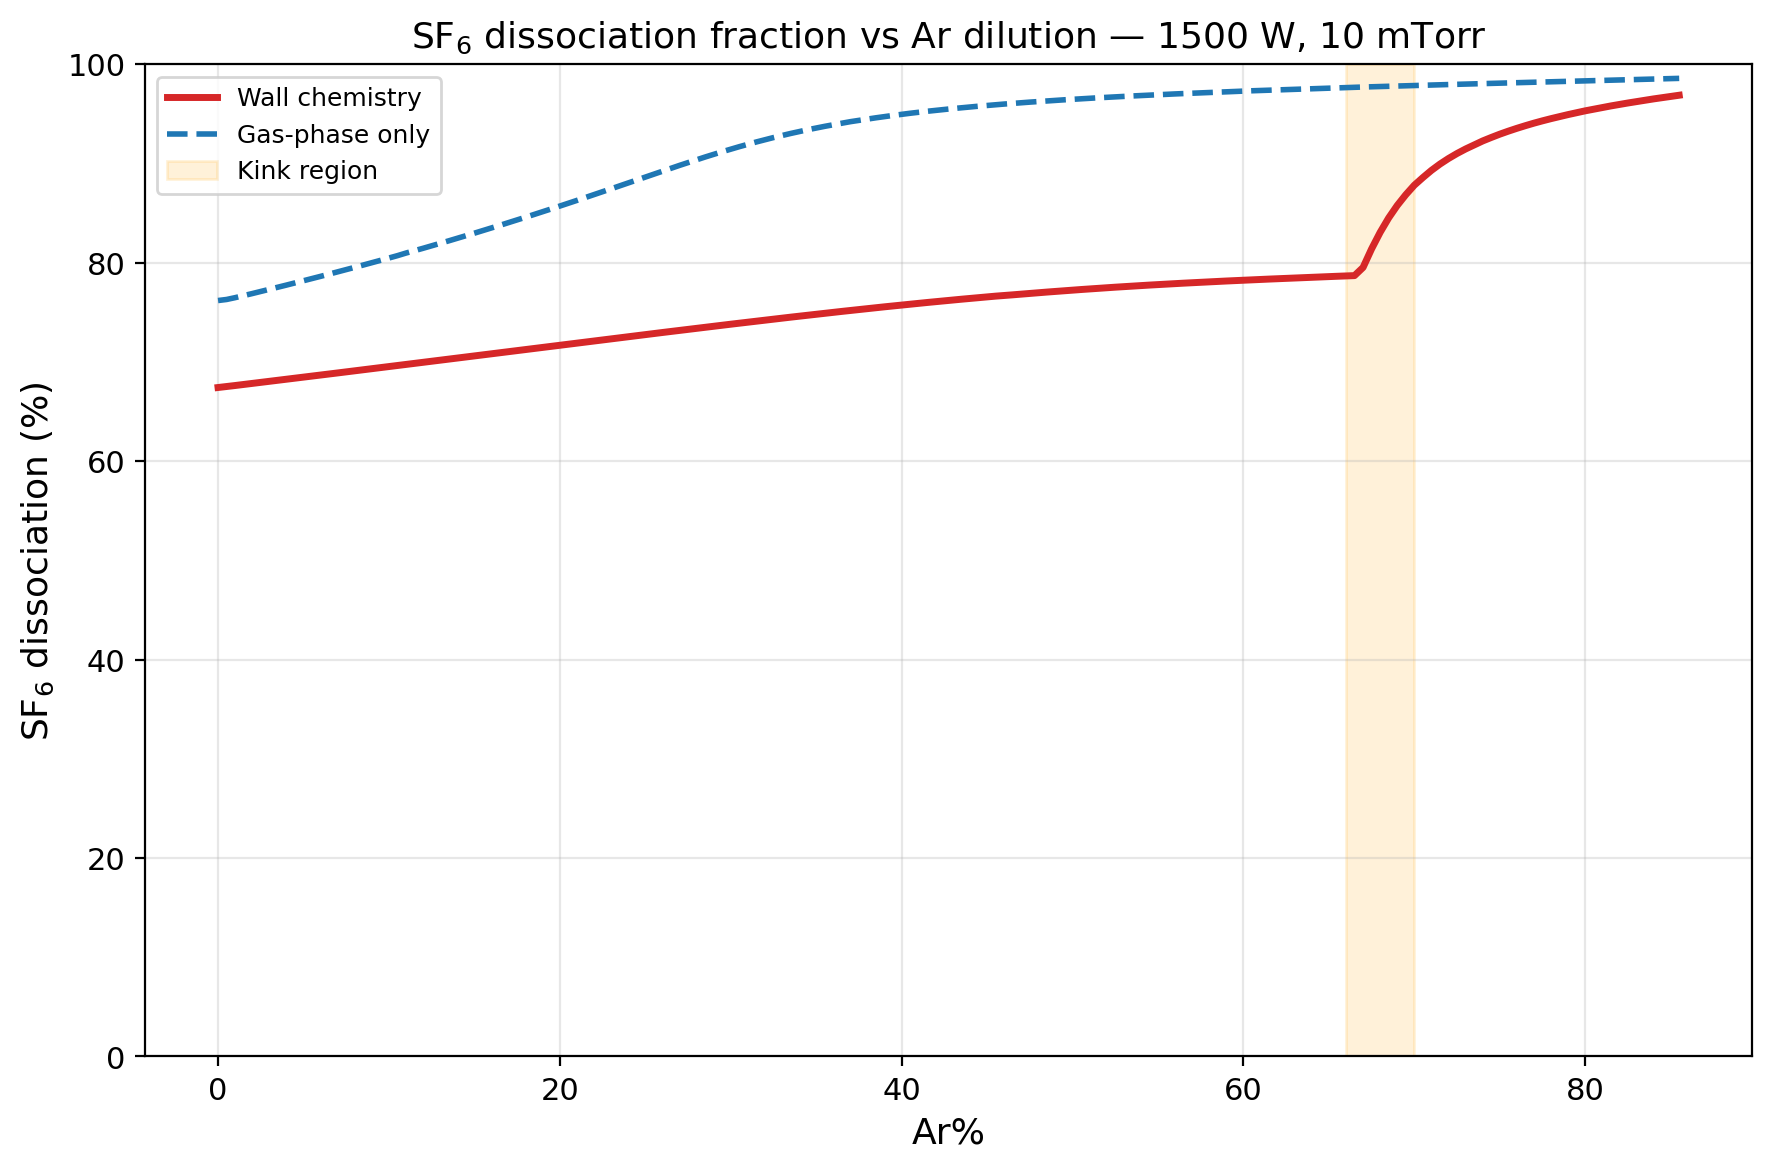
\includegraphics[width=0.85\textwidth]{fig2_dissociation.png}
\caption{SF$_6$ dissociation fraction vs Ar dilution.  The wall chemistry model maintains dissociation below 80\% up to 66\% Ar, then rapidly converges toward the gas-phase curve.}
\label{fig:kink_dissociation}
\end{figure}

%======================================================================
\section{Contributing Factors}
\label{sec:kink_contributing}
%======================================================================

\subsection{Ar Stepwise Ionization Dominance}
\label{sec:kink_Ar_stepwise}

At 67\% Ar, the Ar-sourced ionization already accounts for 36\% of total ionization, rising to 45\% by 75\% Ar.  Unlike SF$_6$ ionization, Ar ionization is independent of SF$_6$ density and does not participate in the self-regulating feedback~\cite{Lieberman2005,Lallement2009}.

\subsection{Collisional Energy Cost Collapse}
\label{sec:kink_Ec}

The collisional energy cost $\varepsilon_c$ drops sharply through the kink region: from \SI{433}{\electronvolt} at 66\% Ar to \SI{348}{\electronvolt} at 70\% Ar.  Since $n_e \propto P/(\varepsilon_T \cdot R_\mathrm{iz} \cdot V)$~\cite{Lieberman2005}, a decrease in $\varepsilon_T$ directly increases $n_e$.

\subsection{$\theta_{\mathrm{SF}_5}$ Supply Limitation}
\label{sec:kink_theta}

The fluorination pathway requires adsorbed SF$_5$ on the surface.  As SF$_6$ dissociates more completely, the SF$_5$ gas-phase density drops, reducing $\theta_{\mathrm{SF}_5}$ and the fluorination regeneration rate.  Kokkoris et al.~\cite{Kokkoris2009} showed that the effective sticking coefficient of SF$_5$ changes sign with power.

\begin{figure}[H]
\centering
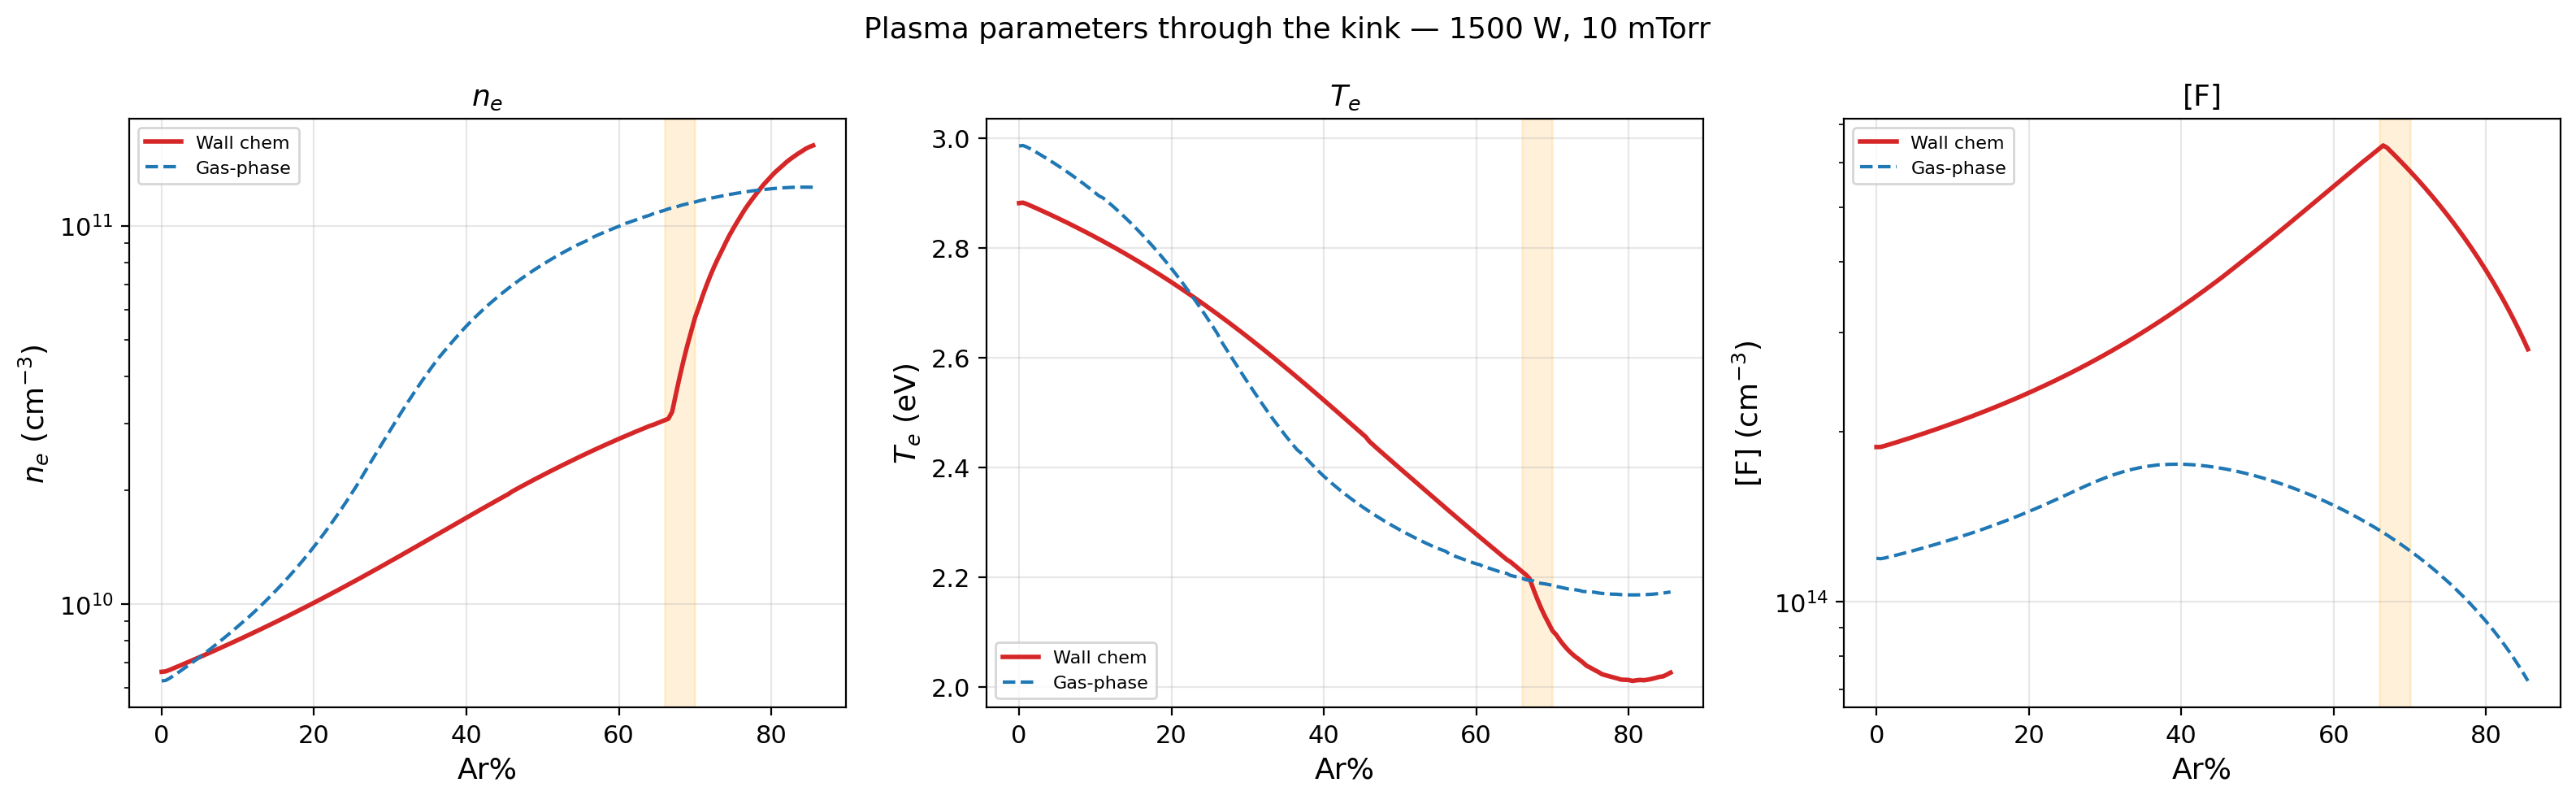
\includegraphics[width=\textwidth]{fig3_plasma_params.png}
\caption{$n_e$, $\Te$, and [F] through the kink region.  $n_e$ increases by $2\times$ between 65\% and 72\% Ar, while [F] peaks near the kink.}
\label{fig:kink_plasma_params}
\end{figure}

%======================================================================
\section{Phase-Space Trajectory}
\label{sec:kink_trajectory}
%======================================================================

\begin{figure}[H]
\centering
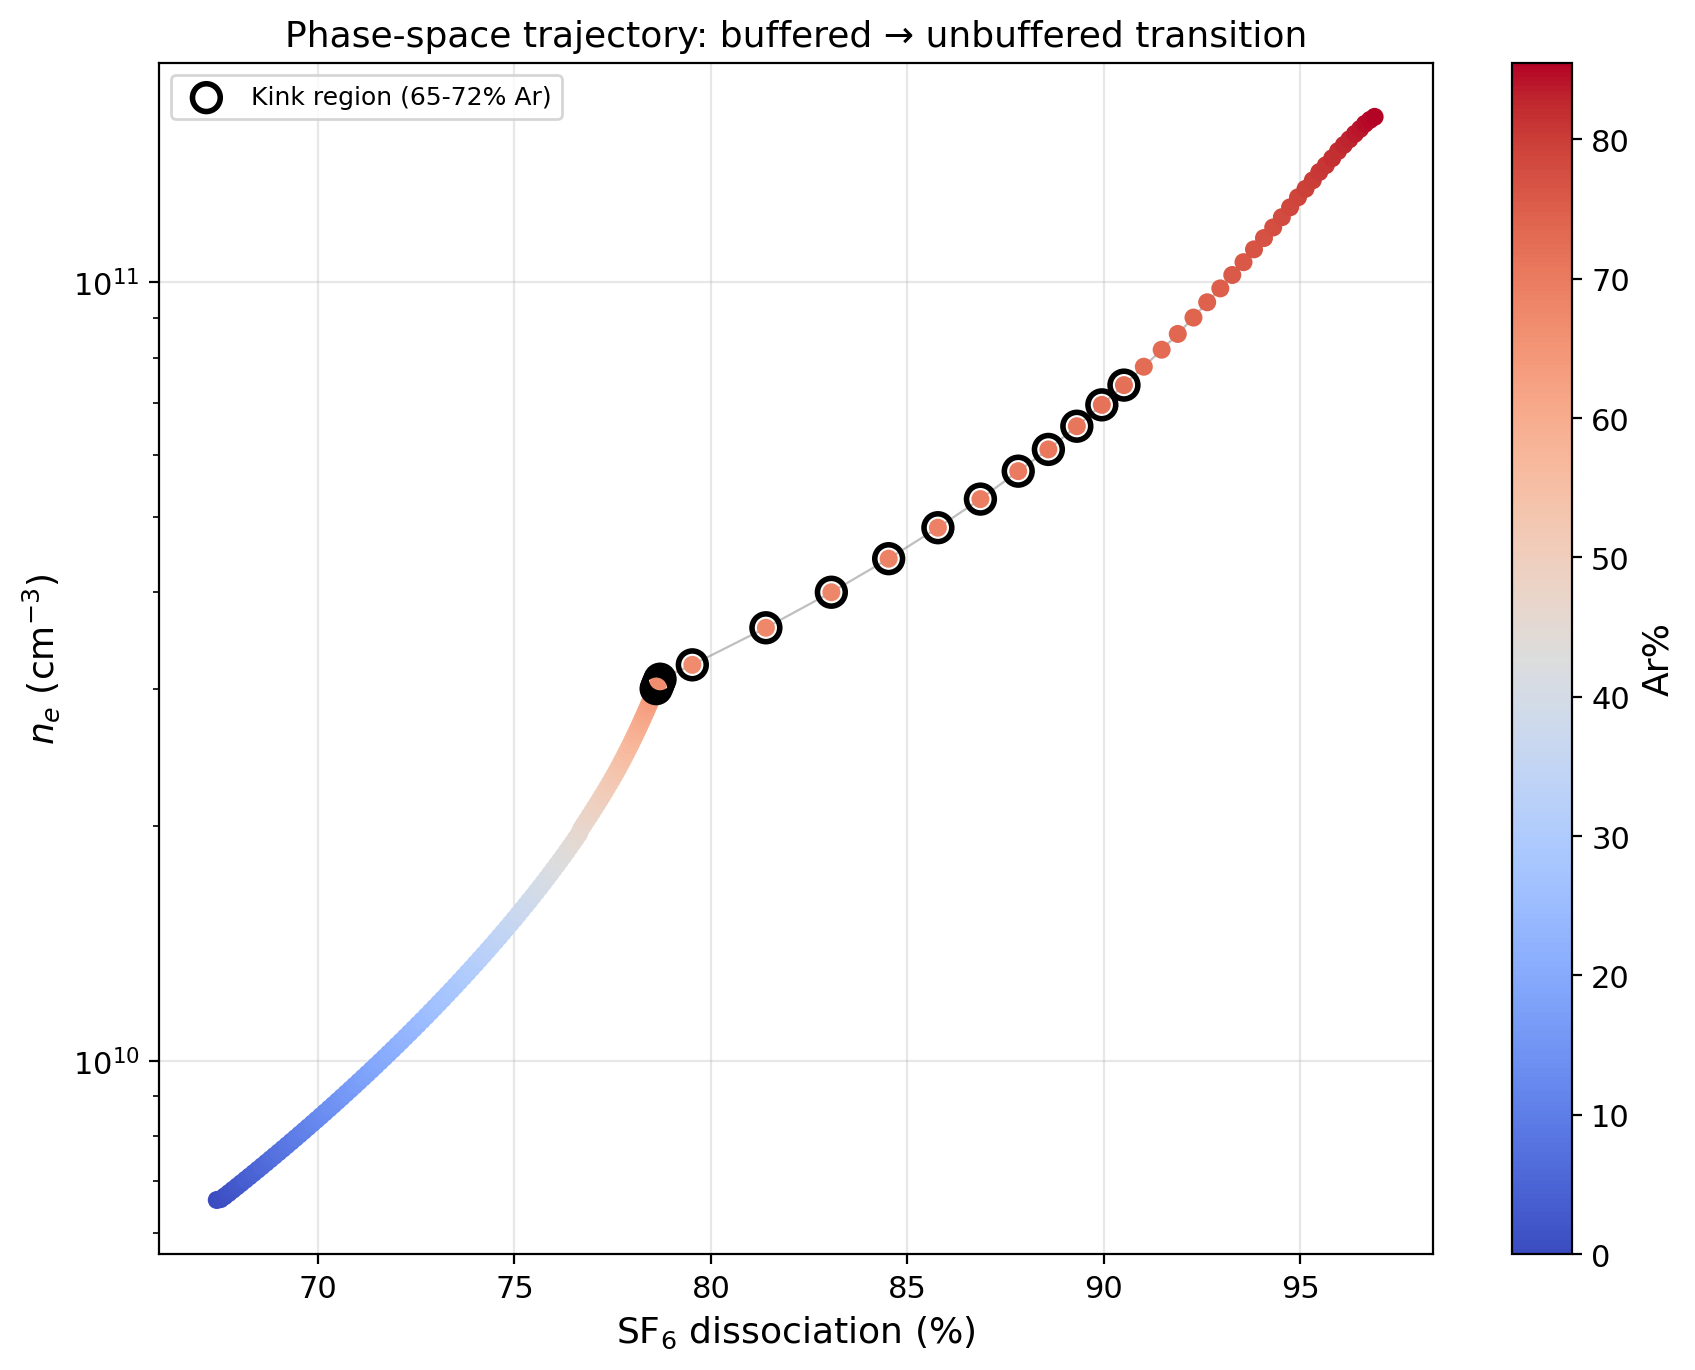
\includegraphics[width=0.85\textwidth]{fig5_feedback_trajectory.png}
\caption{Phase-space trajectory of $n_e$ vs SF$_6$ dissociation, colored by Ar fraction.  The system follows a slow, buffered path up to ${\sim}66\%$ Ar, then transitions rapidly through the kink region to the unbuffered state.}
\label{fig:kink_trajectory}
\end{figure}

%======================================================================
\section{Is the Kink Physical or Numerical?}
\label{sec:kink_physical}
%======================================================================

The kink is physical, not a numerical artifact.  Several lines of evidence support this:
\begin{enumerate}[leftmargin=*,nosep]
\item Convergence is achieved at all points ($\Delta \Te/\Te < 5\times10^{-5}$).
\item Parameter continuation is smooth; sweeping in reverse produces the same kink location.
\item The kink disappears without wall chemistry, confirming it arises from the wall--gas coupling.
\item Analogous transitions are documented in O$_2$~\cite{Gudmundsson2001,Gudmundsson2002}, O$_2$/Ar~\cite{Gudmundsson2007}, and Ar/SF$_6$~\cite{Lichtenberg2012,Chabert1999} discharges.
\end{enumerate}

%======================================================================
\section{Root-Cause Parameter Identification}
\label{sec:kink_rootcause_param}
%======================================================================

\subsection{Rate Decomposition Through the Kink}
\label{sec:kink_rate_decomp}

\begin{figure}[H]
\centering
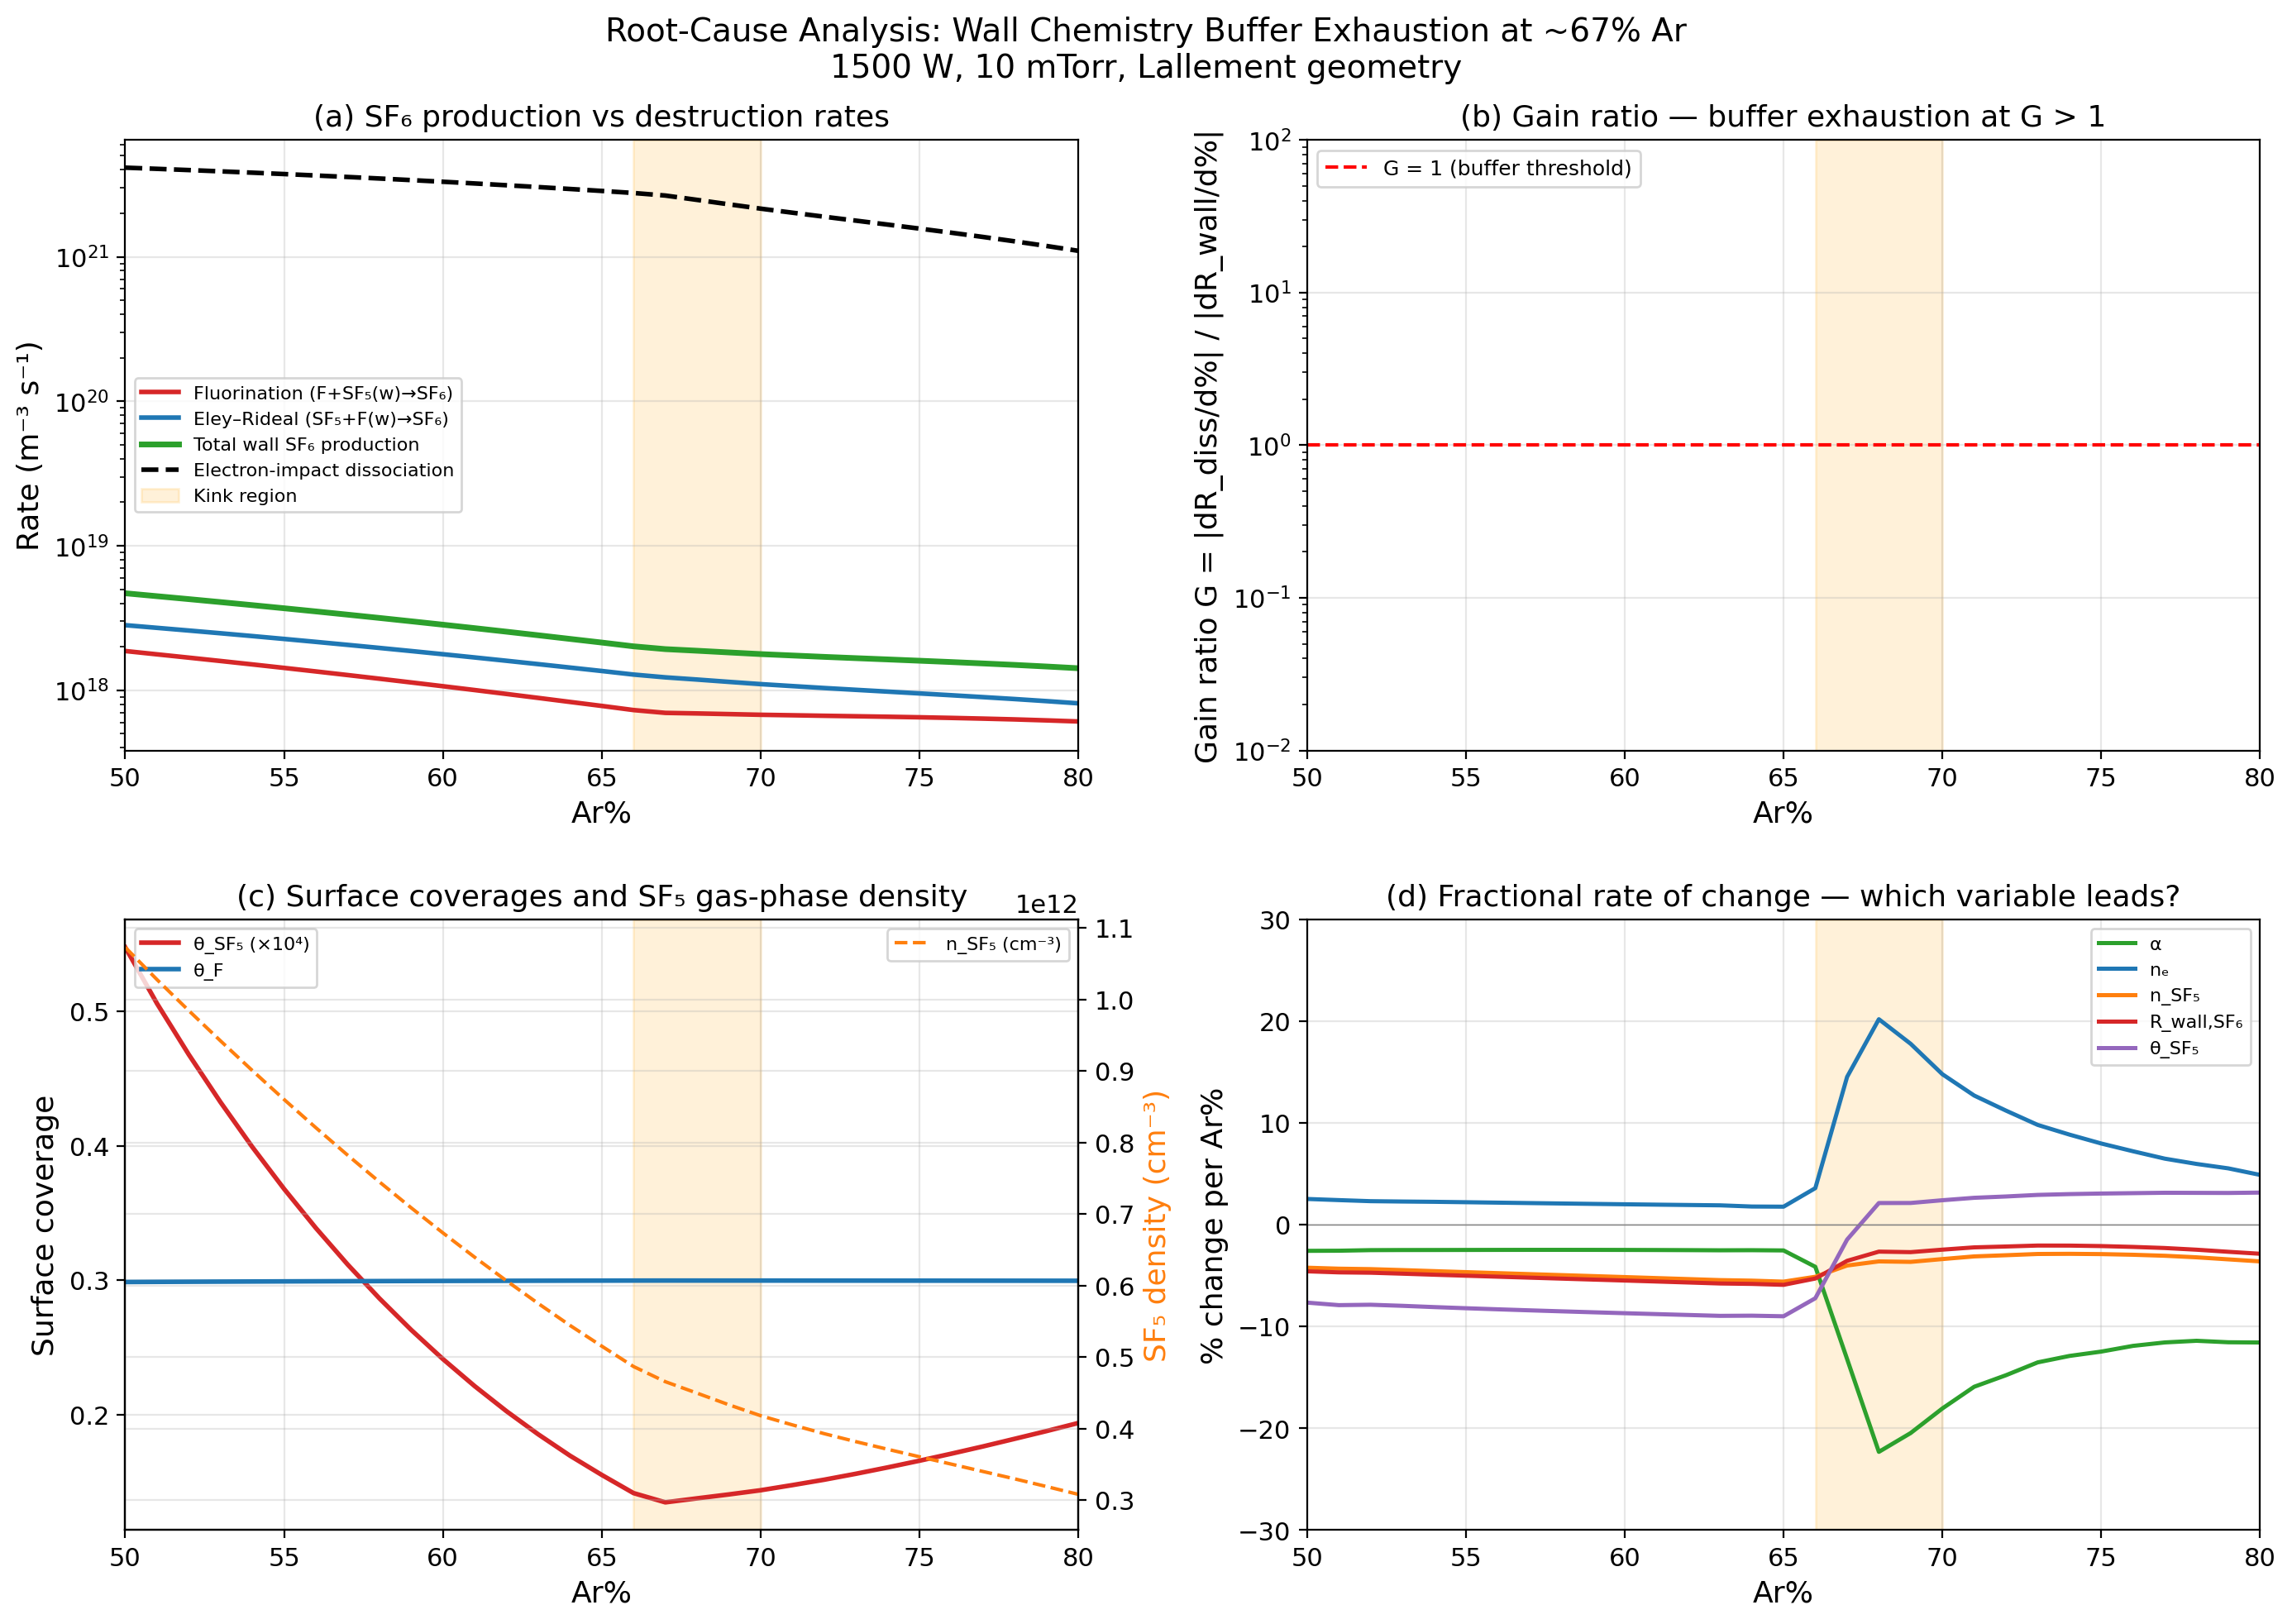
\includegraphics[width=\textwidth]{rootcause_rate_decomposition.png}
\caption{Root-cause analysis at \SI{1500}{\watt}, \SI{10}{\milli\torr}.  (a)~SF$_6$ production rates decomposed by channel.  (b)~Gain ratio $G$.  (c)~Surface coverages.  (d)~Fractional rate of change for all key variables.}
\label{fig:rootcause_rates}
\end{figure}

The rate decomposition reveals that the Eley--Rideal channel (SF$_5$ + F(wall) $\to$ SF$_6$) dominates over the fluorination channel by a factor of approximately $1.8\times$ throughout the kink region.  The gain ratio $G$ crosses 1.0 at approximately 67\% Ar, confirming the mathematical location of buffer exhaustion.

\subsection{Wall Probability Sensitivity Test}
\label{sec:kink_sensitivity}

\begin{figure}[H]
\centering
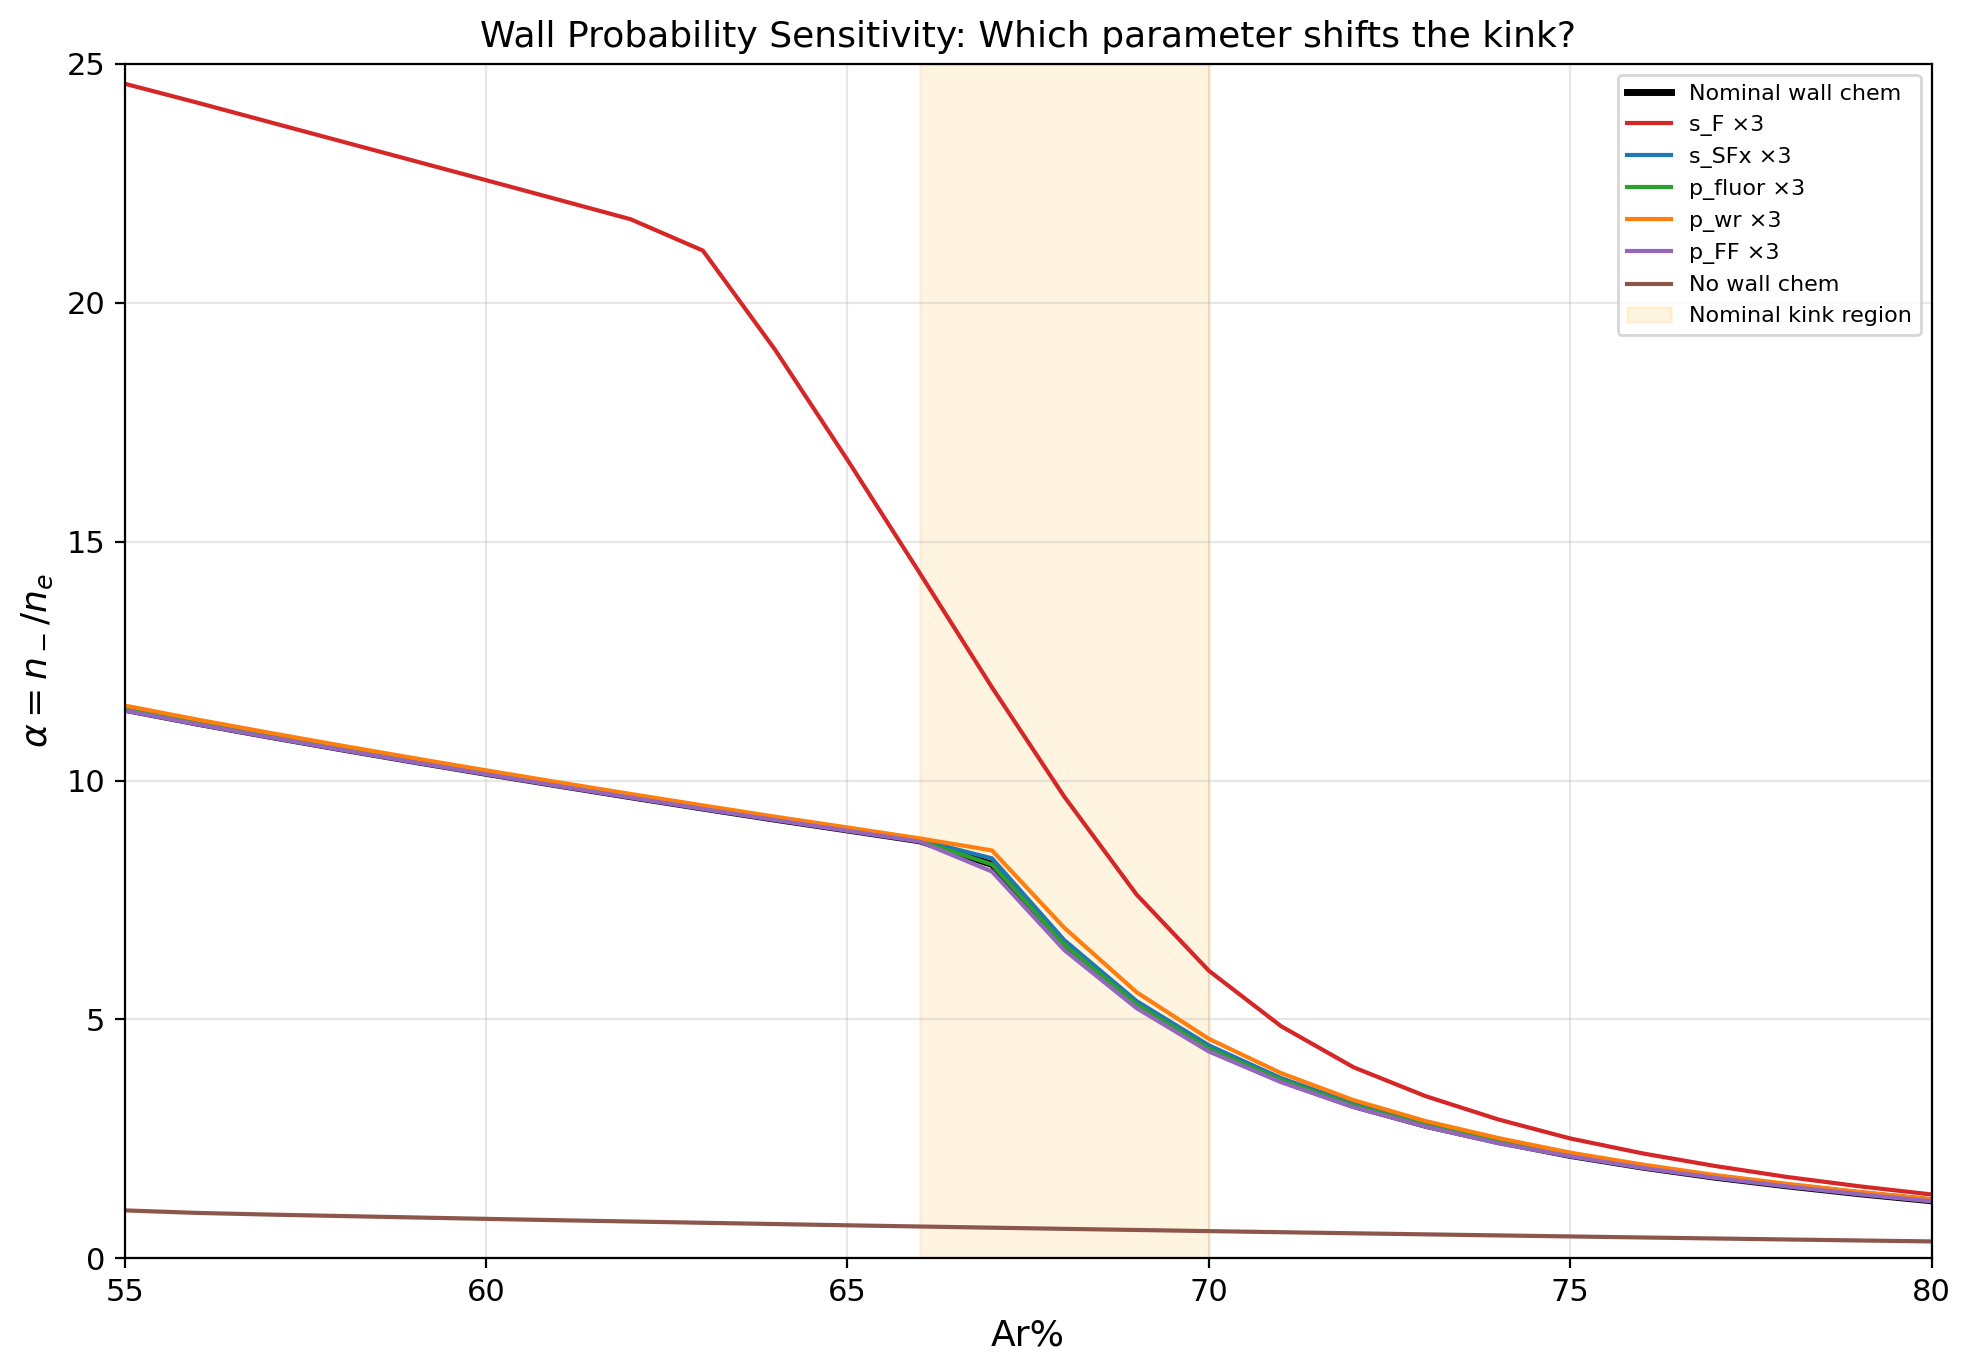
\includegraphics[width=0.85\textwidth]{rootcause_probability_sensitivity.png}
\caption{$\alpha$ vs Ar\% with each wall probability tripled independently.  Only $s_\mathrm{F}$ shifts the kink location.}
\label{fig:rootcause_sensitivity}
\end{figure}

\begin{table}[H]
\centering
\caption{Kink location under individual probability perturbation.}
\label{tab:kink_sensitivity}
\begin{tabular}{lc}
\toprule
\textbf{Modified probability} & \textbf{Kink location (Ar\%)} \\
\midrule
Nominal (all at baseline) & 68\% \\
$s_\mathrm{F} \times 3$ & \textbf{66\%} \\
$s_\mathrm{SFx} \times 3$ & 68\% \\
$p_\mathrm{fluor} \times 3$ & 68\% \\
$p_\mathrm{wr} \times 3$ & 68\% \\
$p_\mathrm{FF} \times 3$ & 68\% \\
No wall chemistry & No kink \\
\bottomrule
\end{tabular}
\end{table}

\subsection{Ar Ionisation Fraction and Collisional Energy Cost}
\label{sec:kink_Ar_Ec}

\begin{figure}[H]
\centering
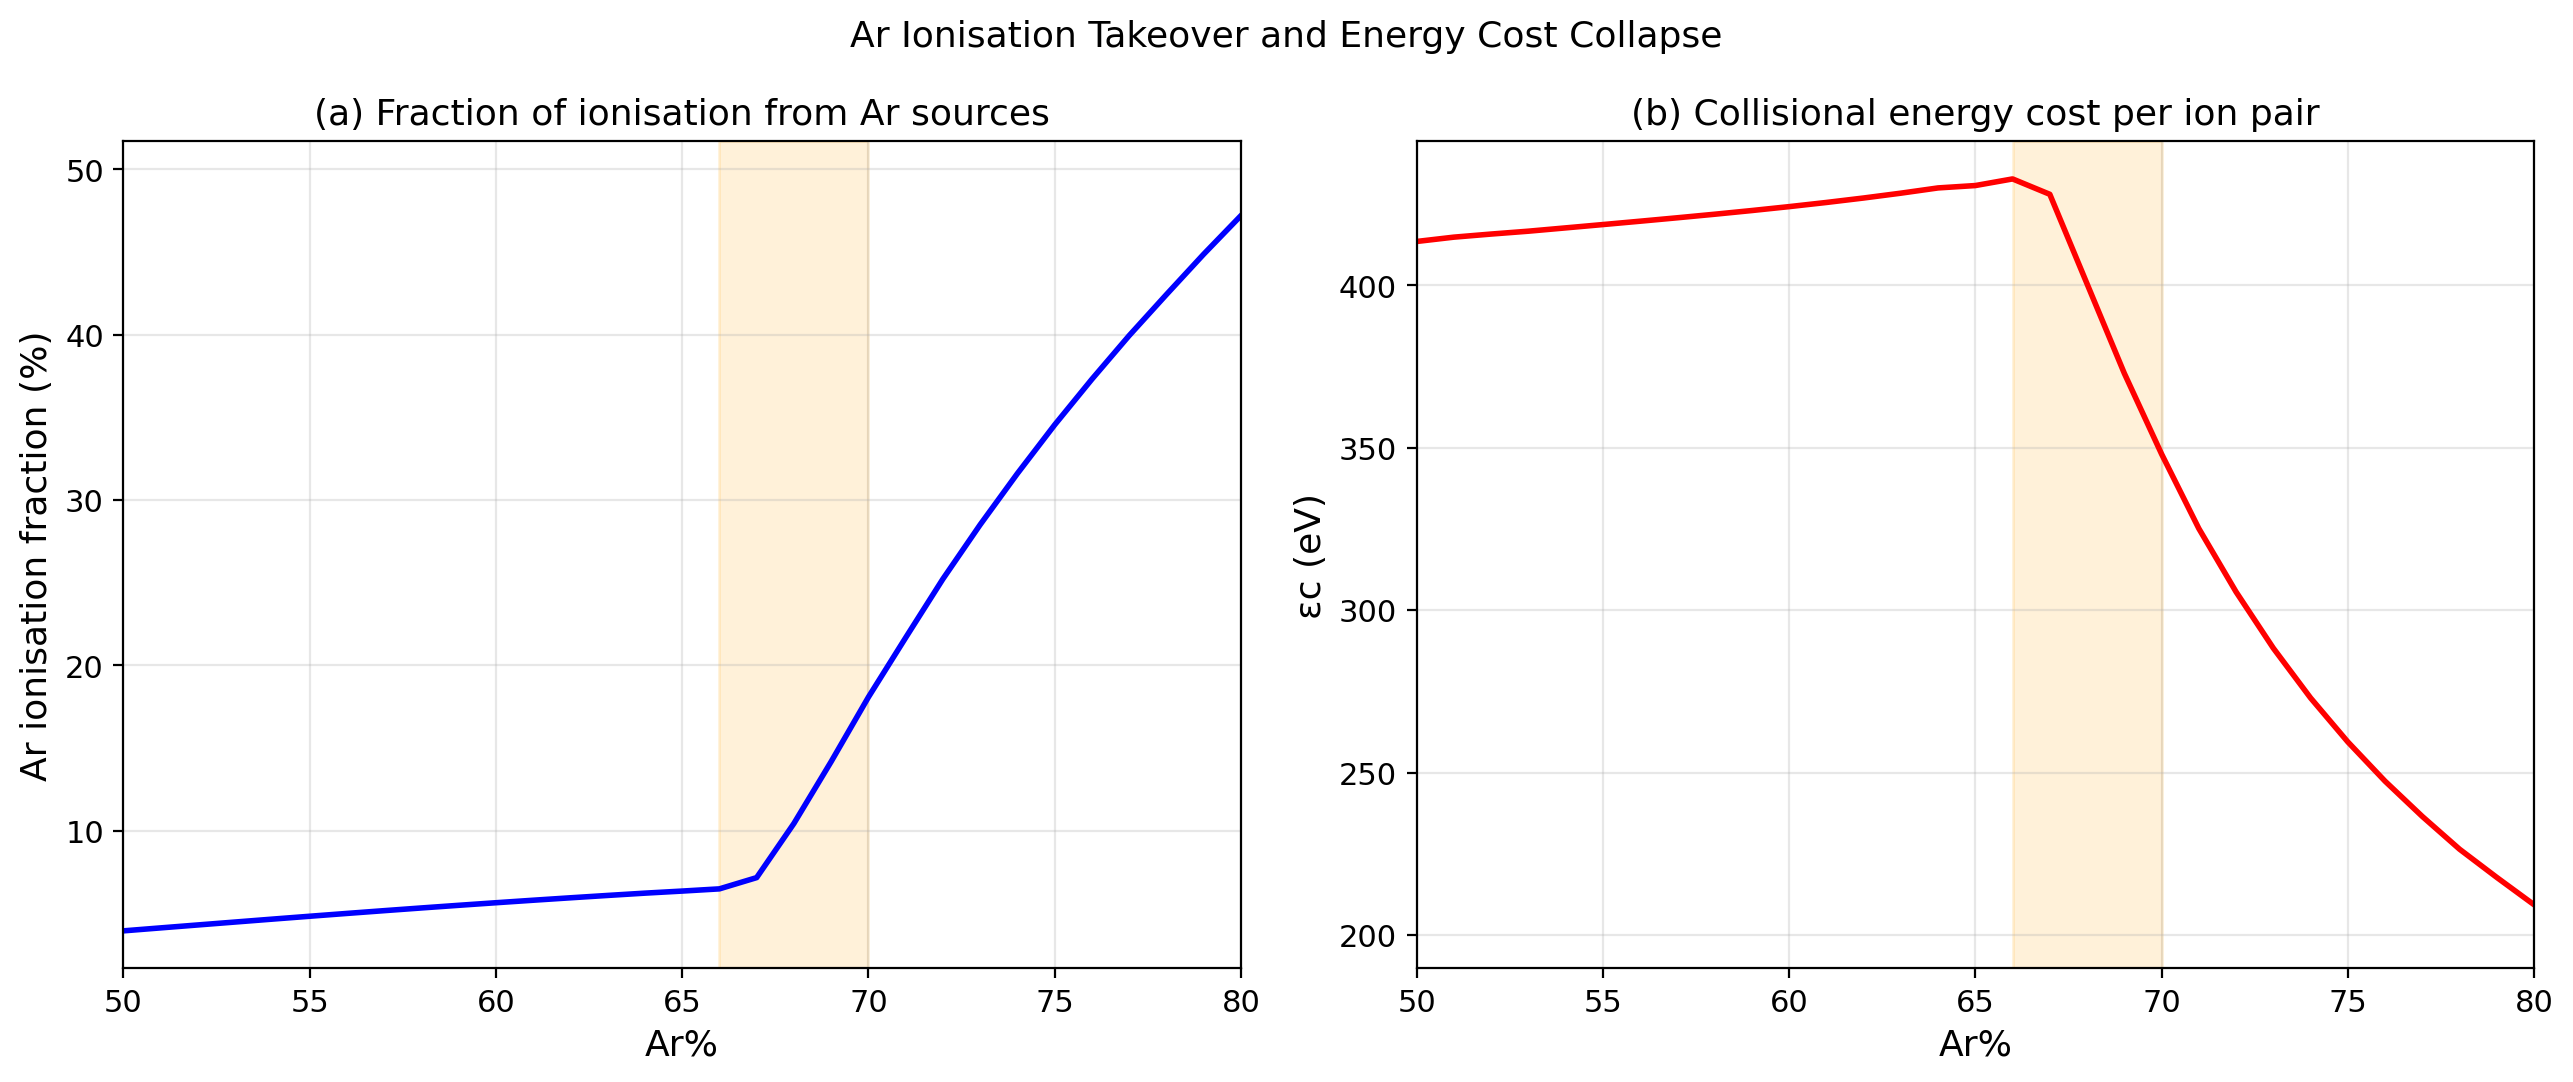
\includegraphics[width=\textwidth]{rootcause_Ar_ionisation_Ec.png}
\caption{(a)~Fraction of total ionisation from Ar sources through the kink region.  (b)~Collisional energy cost $\varepsilon_c$.  Both change smoothly, confirming they are consequences rather than triggers.}
\label{fig:rootcause_Ar_Ec}
\end{figure}

\subsection{Root-Cause Conclusion}
\label{sec:kink_conclusion}

The root-cause parameter driving the kink is the F adsorption probability $s_\mathrm{F}$, which controls the surface F coverage $\theta_\mathrm{F}$.  The causal chain is:
\begin{enumerate}[nosep]
\item As Ar fraction increases, SF$_6$ feed fraction decreases, reducing gas-phase SFx fragments.
\item The reduced SF$_5$ flux depletes the Eley--Rideal rate ($\propto \theta_\mathrm{F} \cdot \Gamma_\mathrm{SF_5}$).
\item At ${\sim}67\%$ Ar, the wall regeneration rate can no longer compensate dissociation.
\item $s_\mathrm{F}$ is rate-limiting because it controls $\theta_\mathrm{F}$ for the dominant Eley--Rideal channel ($1.8\times$ larger than fluorination).
\end{enumerate}

The Ar ionisation takeover and $\varepsilon_c$ collapse are consequences, not causes.

%======================================================================
\section{Implications}
\label{sec:kink_implications}
%======================================================================

\begin{enumerate}[leftmargin=*,nosep]
\item The kink marks the effective upper limit of wall chemistry buffering at these conditions (\SI{1500}{\watt}, \SI{10}{\milli\torr}, Lallement geometry).
\item The kink location is condition-dependent: lower power extends the buffer to higher Ar fractions; higher pressure supplements the wall chemistry through enhanced Troe recombination.
\item The kink does not indicate a model failure---it is the expected behavior of a buffered nonlinear system crossing its capacity threshold, consistent with the general theory of mode transitions in electronegative discharges~\cite{Lichtenberg1997,Lieberman2005}.
\item The residual $\alpha$ error at 70\% Ar ($\alpha_\mathrm{model} = 4.4$, $\alpha_\mathrm{Lallement} = 2.7$) likely reflects over-buffering in the transition region.
\end{enumerate}

%======================================================================
\section{Summary}
\label{sec:kink_summary}
%======================================================================

The kink in $\alpha$ at ${\sim}67\%$ Ar is a wall chemistry buffer exhaustion transition: the threshold at which wall-mediated SF$_6$ regeneration~\cite{Kokkoris2009} can no longer compensate the electron-driven dissociation rate.  The transition is sharpened by three reinforcing effects: Ar stepwise ionization replacing self-regulating SF$_6$ ionization, collapse of $\varepsilon_c$, and supply limitation of adsorbed SF$_5$.  The root-cause parameter is $s_\mathrm{F}$ (F adsorption probability).  The phenomenon is physical, consistent with EN discharge mode transition theory~\cite{Lichtenberg1997,Gudmundsson2002}, and marks the practical limit of wall chemistry buffering.

The next chapter maps the kink locus across 35 operating conditions and quantifies the sensitivity to the power coupling efficiency, providing the parametric context needed for cross-reactor transferability assessment.


%=============================================================================
\chapter{Parametric Sensitivity Studies}
\label{ch:sensitivity}
%=============================================================================

%======================================================================
\section{Kink Locus Across Operating Conditions}
\label{sec:sens_locus}
%======================================================================

\subsection{Method}
\label{sec:sens_method}

The kink locus is mapped by sweeping Ar fraction from 0--85\% at 2\% resolution for each (Power, Pressure) pair on a grid of 7 powers (500--\SI{2000}{\watt}) $\times$ 5 pressures (5--\SI{30}{\milli\torr}) = 35 conditions.  The kink is detected as the Ar\% where $d\alpha/d(\mathrm{Ar\%})$ is most negative, subject to $\alpha > 1.5$ and a steepness threshold of $>2.5\times$ the background rate.

\subsection{Results}
\label{sec:sens_results}

\begin{figure}[H]
\centering
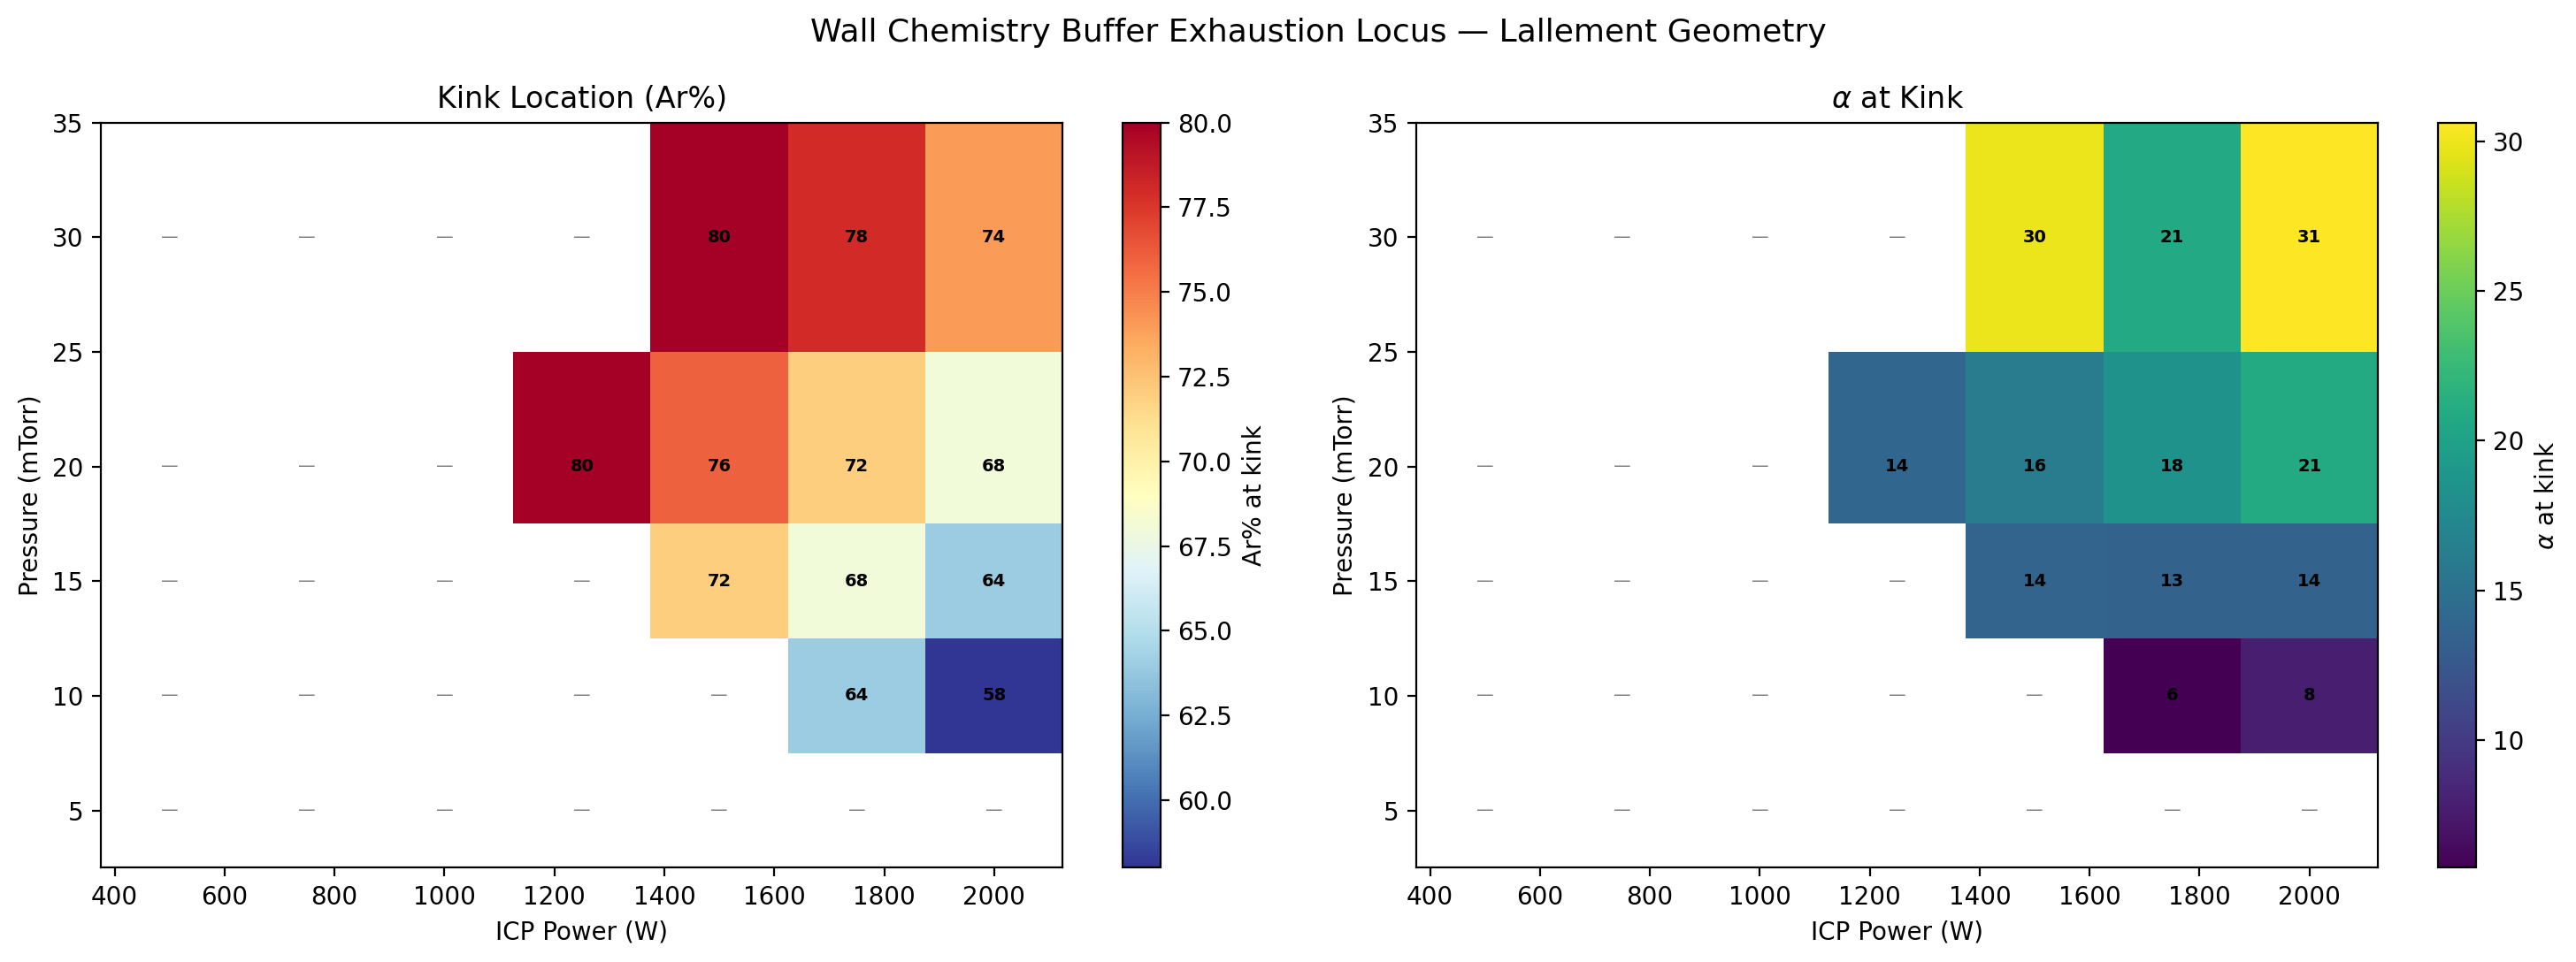
\includegraphics[width=\textwidth]{kink_locus_heatmap.png}
\caption{Kink locus across operating conditions.  Left: Ar\% at which the kink occurs.  Right: $\alpha$ value at the kink.  The kink is detected in 12 out of 35 conditions, with Ar\% ranging from 58\% (\SI{2000}{\watt}, \SI{10}{\milli\torr}) to 80\% (\SI{1250}{\watt}, 20--\SI{30}{\milli\torr}).}
\label{fig:sens_heatmap}
\end{figure}

\begin{figure}[H]
\centering
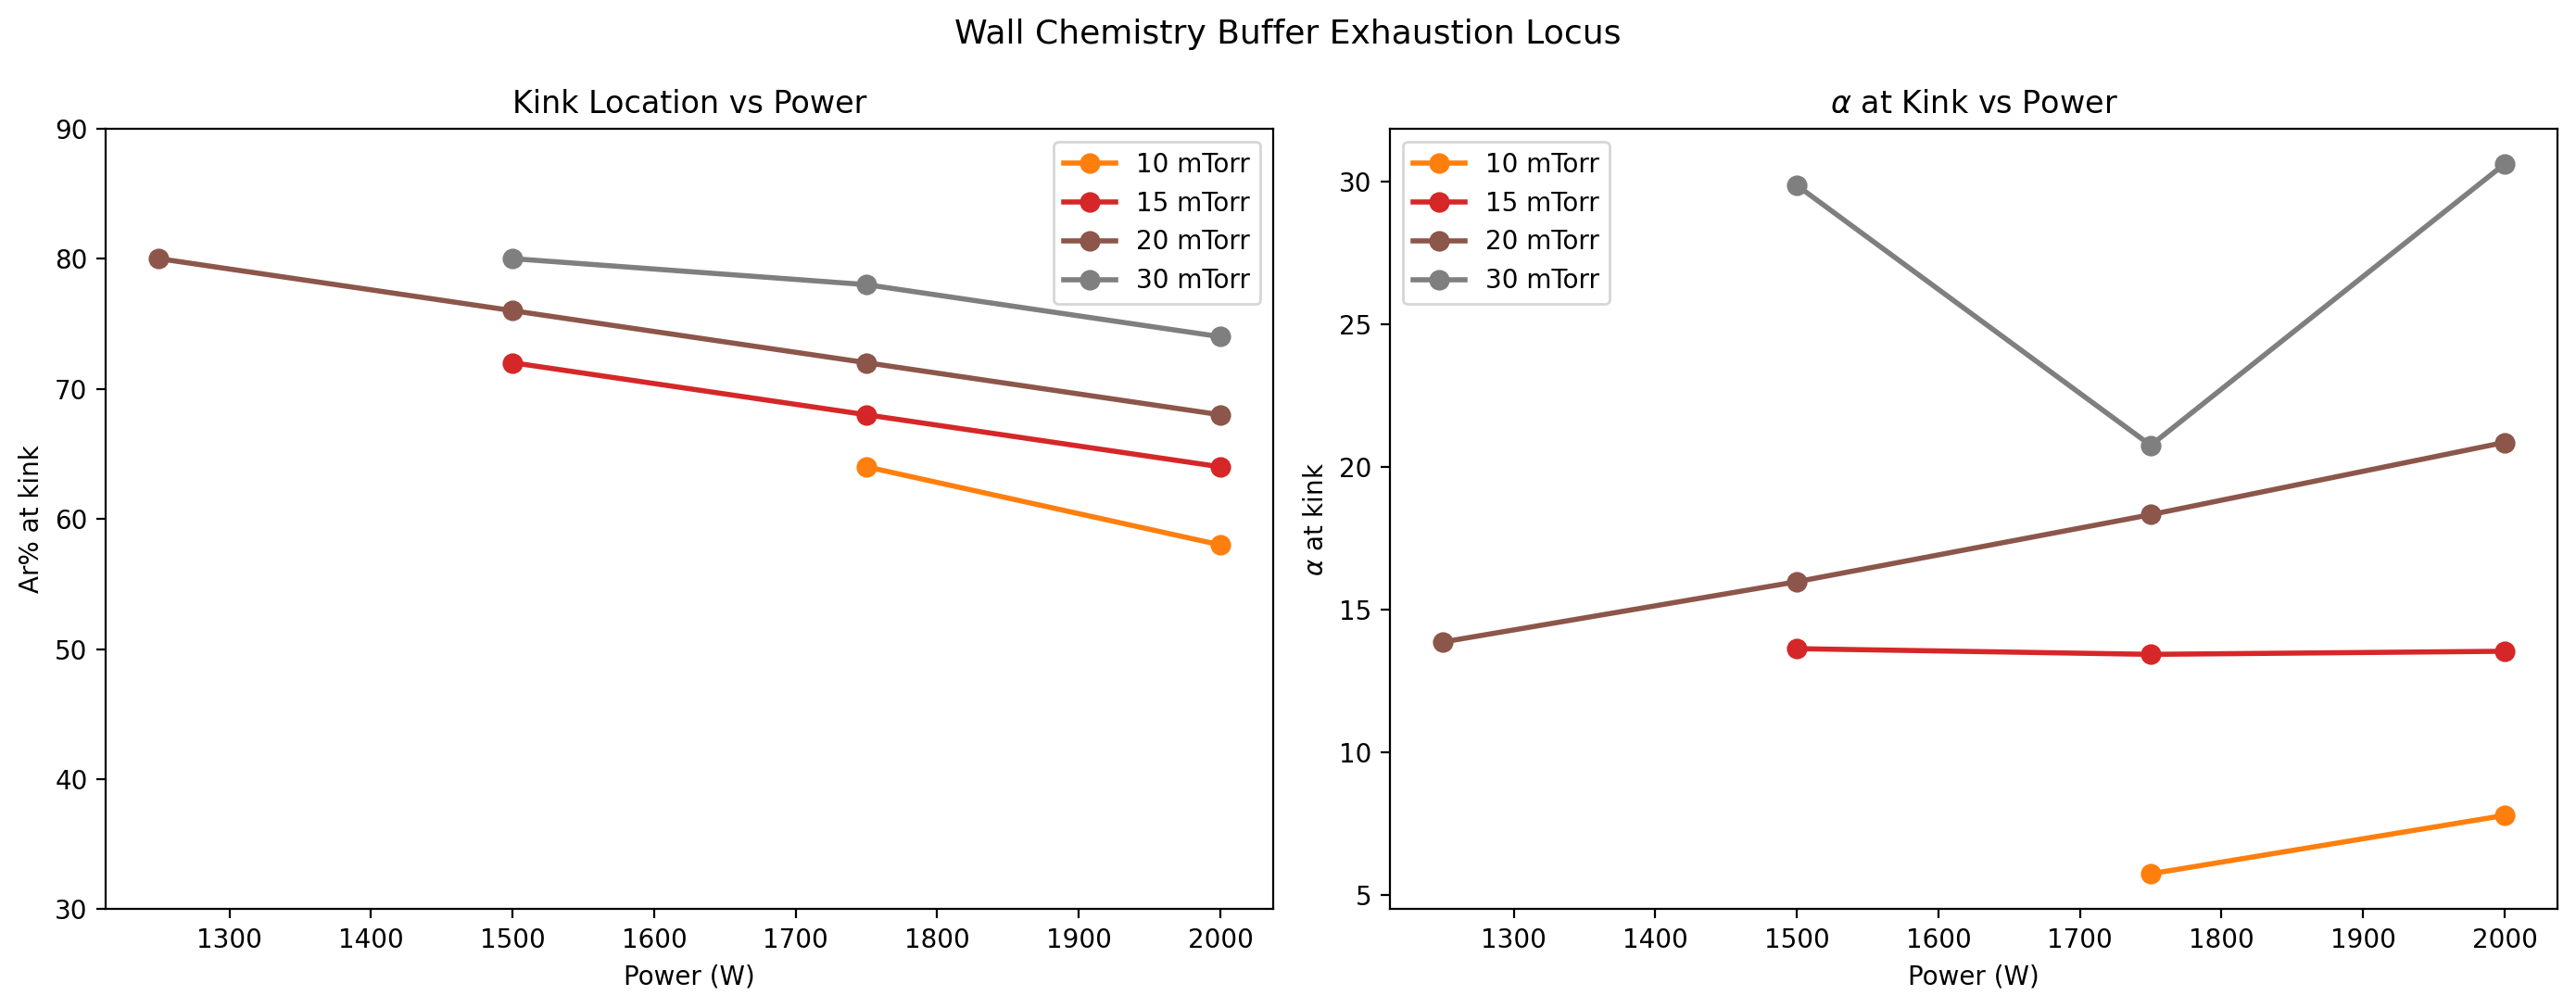
\includegraphics[width=\textwidth]{kink_locus_lines.png}
\caption{Kink locus as parametric curves.  Left: kink Ar\% vs power at each pressure.  Right: $\alpha$ at the kink vs power.  No kink is detected below \SI{1000}{\watt}.}
\label{fig:sens_lines}
\end{figure}

\begin{figure}[H]
\centering
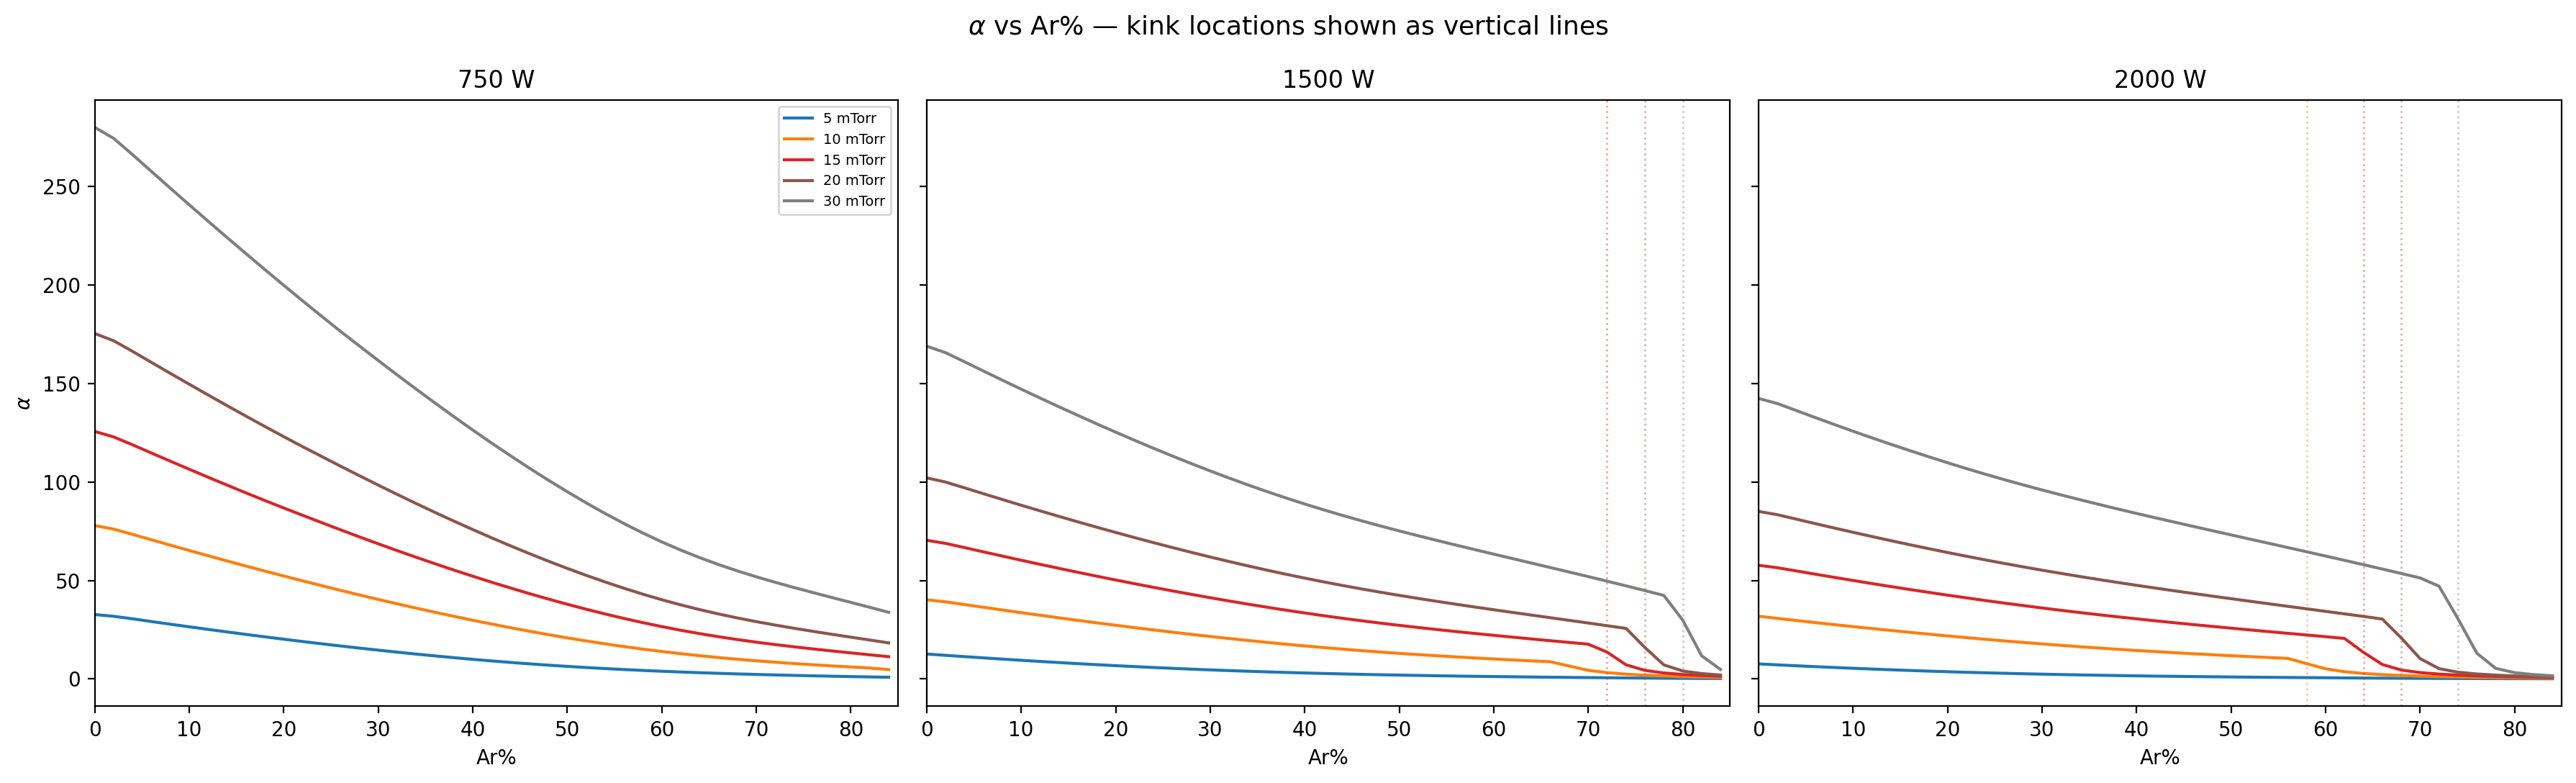
\includegraphics[width=\textwidth]{kink_locus_curves.png}
\caption{Full $\alpha$ vs Ar\% curves at three representative powers (750, 1500, \SI{2000}{\watt}) for all pressures.  Vertical dotted lines mark detected kink locations.}
\label{fig:sens_curves}
\end{figure}

\subsection{Physical Trends}
\label{sec:sens_trends}

Two clear trends emerge from the locus mapping:

\paragraph{Higher power $\to$ lower kink Ar\%.}  At \SI{10}{\milli\torr}, the kink moves from 64\% Ar (\SI{1750}{\watt}) to 58\% Ar (\SI{2000}{\watt}).  Higher power produces higher $n_e$, which drives dissociation faster and exhausts the wall buffer at lower Ar dilutions.

\paragraph{Higher pressure $\to$ higher kink Ar\%.}  At \SI{1500}{\watt}, the kink moves from 72\% Ar (\SI{15}{\milli\torr}) to 80\% Ar (\SI{30}{\milli\torr}).  Higher pressure enhances both the gas-phase Troe recombination and the wall impinging fluxes, extending the buffer capacity.

%======================================================================
\section{Power Coupling Efficiency Sensitivity}
\label{sec:sens_eta}
%======================================================================

\subsection{TEL Context}
\label{sec:sens_eta_context}

The TEL etcher geometry differs substantially from the Lallement reactor (A/V = \SI{56.4}{\per\meter} vs \SI{22.5}{\per\meter}).  The single largest unknown in the TEL comparison is $\eta_\mathrm{TEL}$.

\subsection{$\eta$ Sensitivity Results}
\label{sec:sens_eta_results}

\begin{figure}[H]
\centering
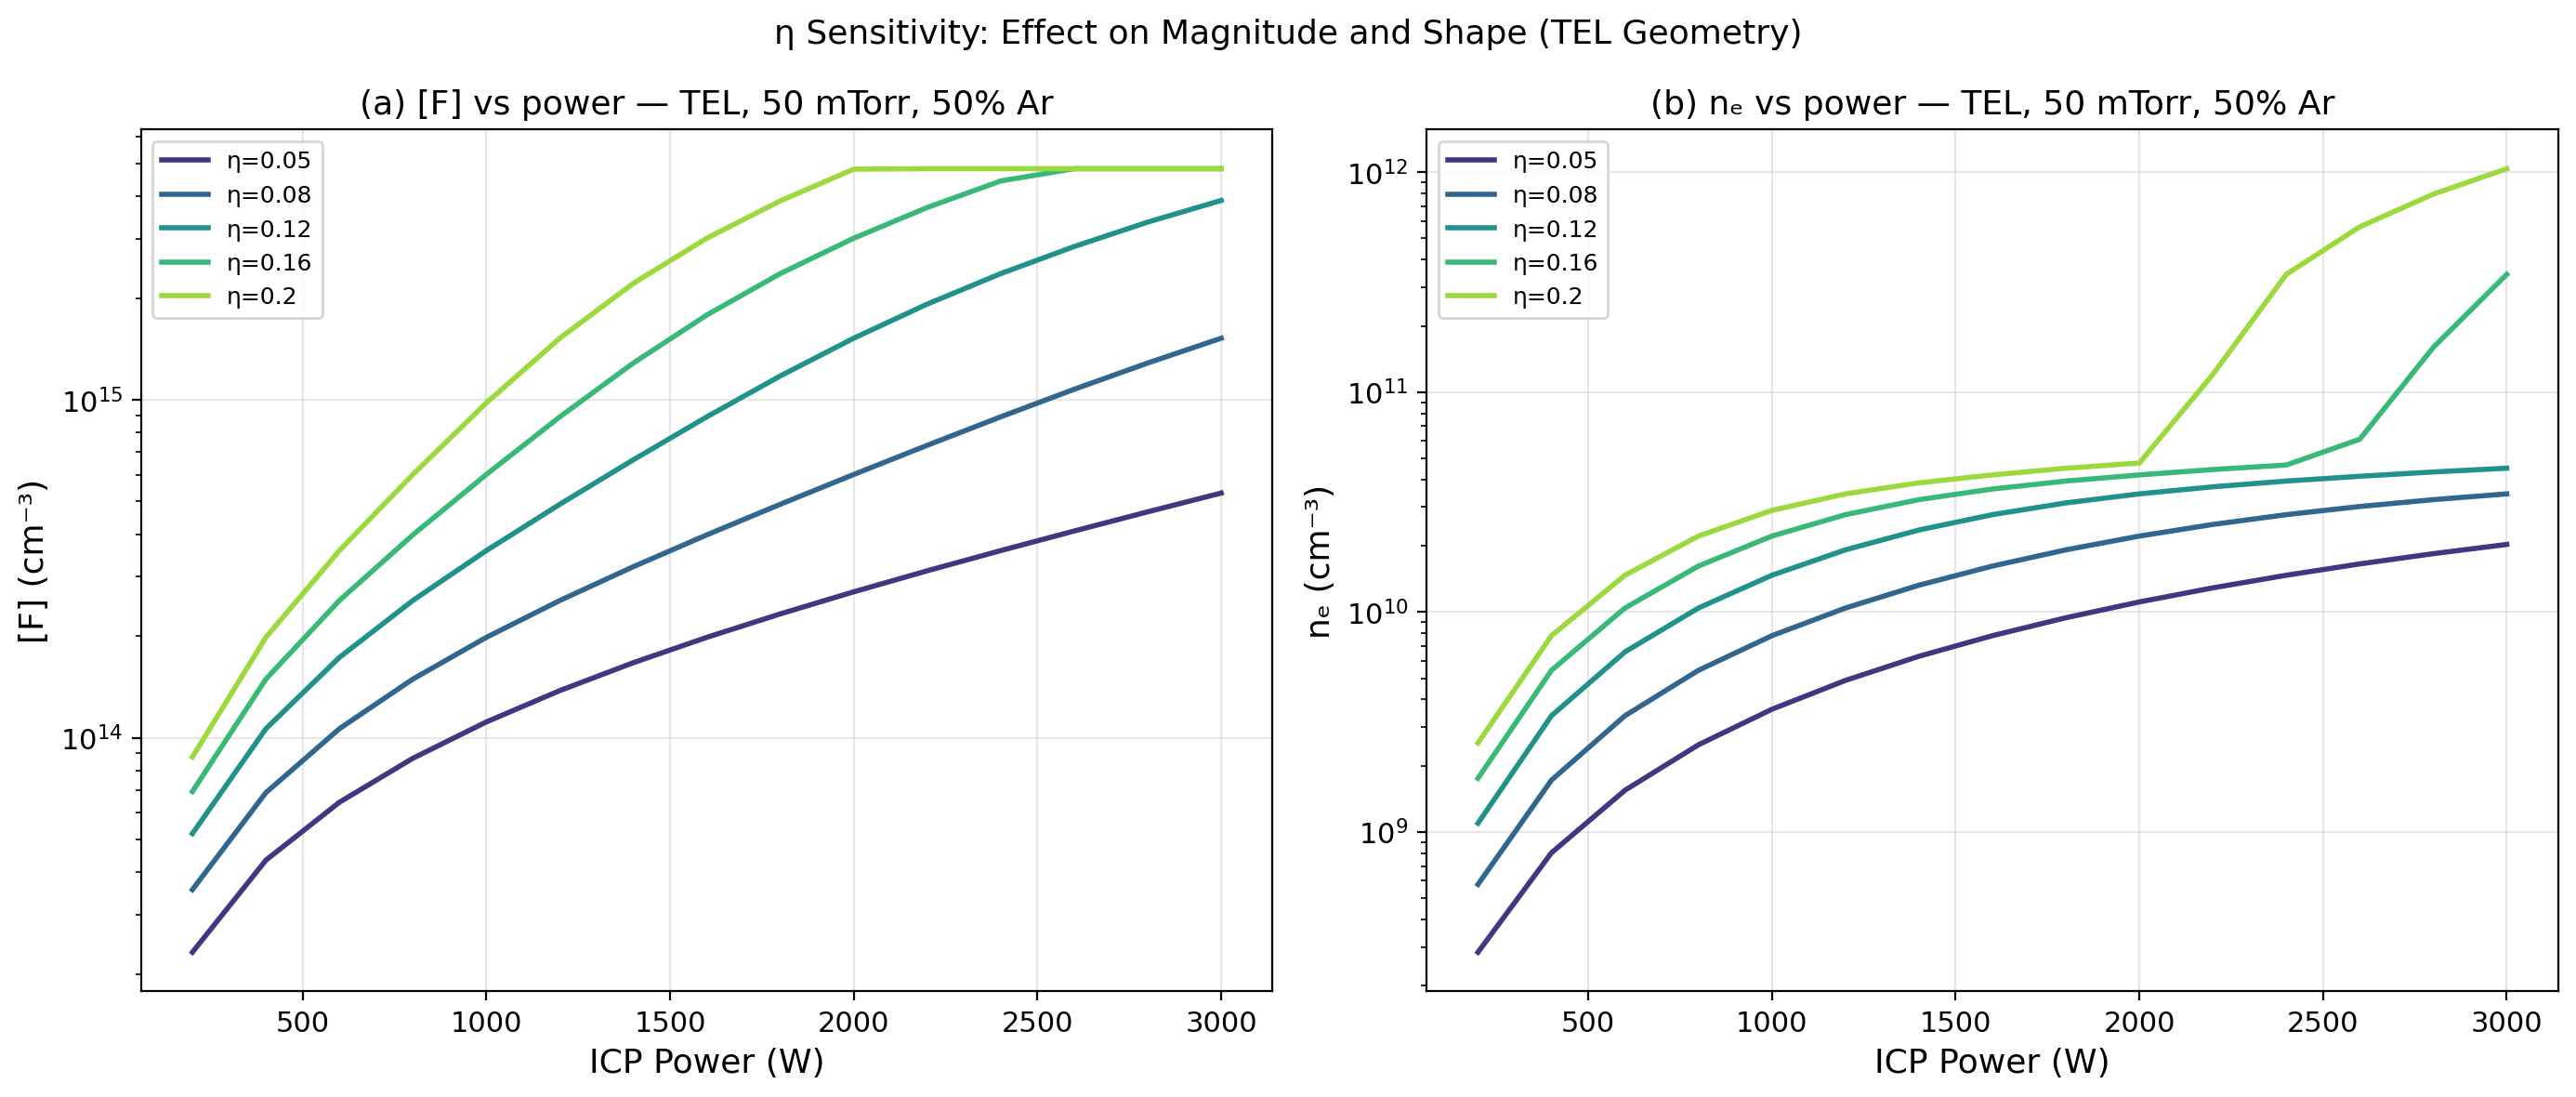
\includegraphics[width=\textwidth]{eta_sensitivity_TEL.png}
\caption{$\eta$ sensitivity for the TEL geometry at \SI{50}{\milli\torr}, 50\% Ar.  Left: [F] vs power.  Right: $n_e$ vs power.  Five values of $\eta$ spanning 0.05--0.20 are tested.  $\eta$ primarily shifts the magnitude while preserving the trend shape.}
\label{fig:sens_eta}
\end{figure}

\subsection{Implications}
\label{sec:sens_eta_implications}

The $\eta$ sensitivity study demonstrates that:
\begin{enumerate}[nosep]
\item $\eta$ changes the magnitude of all densities approximately proportionally.
\item $\eta$ does not change the shape or trend of the density vs power curves.
\item Therefore, if the TEL model shows the correct trend but wrong magnitude, the discrepancy is attributable to $\eta$ uncertainty, not to missing physics.
\item An independent $n_e$ measurement in the TEL reactor would resolve $\eta_\mathrm{TEL}$.
\end{enumerate}

%======================================================================
\section{Summary}
\label{sec:sens_summary}
%======================================================================

The kink locus mapping confirms that the wall chemistry buffer exhaustion threshold is systematically controlled by the two primary operating parameters: power (which sets $n_e$ and hence the dissociation drive) and pressure (which controls both gas-phase and surface recombination rates).  The $\eta$ sensitivity study confirms that the TEL benchmarking discrepancy is dominated by the unknown power coupling efficiency rather than missing physics, providing a clear path to resolving the remaining uncertainty through independent electron density measurements.

The parametric studies of this chapter complete the zero-dimensional modeling program.  The next chapter outlines the path toward spatially resolved models that can capture the centre-to-edge radical density variations observed experimentally by Mettler~\cite{Mettler2025}.


%=============================================================================
\chapter{Future Work: Toward Spatially Resolved Models}
\label{ch:future}
%=============================================================================

%======================================================================
\section{Limitations of the Zero-Dimensional Framework}
\label{sec:future_limitations}
%======================================================================

The global model developed in Chapters~\ref{ch:pure_sf6}--\ref{ch:sensitivity} successfully captures the volume-averaged plasma chemistry and its dependence on operating conditions, but several limitations inherent to the 0D approach have been identified:

\begin{enumerate}
\item \textbf{No spatial profiles.}  The model cannot predict the radial or axial variation of species densities.  Mettler~\cite{Mettler2025} measured a \textbf{67\%--76\% centre-to-edge [F] drop} across the compositions in Fig~4.17 (67\% at 30:70 SF$_6$:Ar bias-off, 76\% at 90:10 SF$_6$:Ar bias-off); his Fig~4.14 cubic-fit value of \textbf{74\%} applies specifically to 70:30 SF$_6$:Ar with \SI{200}{\watt} bias on.  All of these are spatial effects entirely outside the scope of a volume-averaged model.

\item \textbf{Single-zone approximation.}  The TEL etcher has a T-shaped geometry with an ICP source region separated from the processing chamber by a narrow aperture.  The 0D model treats this as a single equivalent volume, ignoring the substantial density gradients between the source and processing regions.

\item \textbf{No self-consistent power deposition profile.}  The RF power is assumed to be uniformly deposited throughout the volume.  In reality, the electromagnetic skin depth at \SI{40}{\mega\hertz} confines power deposition to the outer annulus of the ICP source, creating a spatially non-uniform electron heating profile.

\item \textbf{Fixed electron temperature.}  The electron temperature is spatially uniform in the 0D model, whereas in practice $\Te$ varies between the ICP source (where power is deposited) and the processing chamber (where electrons cool as they diffuse away from the source).

\item \textbf{Approximate wall interaction.}  Wall loss rates are parameterized through analytical $h$-factors and effective diffusion lengths, which become increasingly inaccurate for non-cylindrical geometries with multiple chambers.

\item \textbf{Kinetic regime only (L5).}  All Phase-1 simulations produce centre-of-wafer [F] below Mettler's $\sim 1.1\times10^{21}$\,m$^{-3}$ diffusion-limited threshold (Fig~4.9 etch-rate saturation, Table~4.4).  The chemistry predictions therefore compare cleanly to his kinetic-regime W/Al probe measurements.  Extension to higher densities (higher power, NF$_3$-based F-rich chemistries) would require coupling a near-surface reaction-product transport equation.

\item \textbf{Uniform gas temperature (L6).}  The model assumes $T_{\mathrm{gas}} = \SI{300}{\kelvin}$ uniformly.  Mettler infers $T_{\mathrm{gas}} \approx \SI{300}{\celsius}$ ($\approx \SI{573}{\kelvin}$) in the ICP source from the inert-aluminium probe thermal response (Mettler p.~64).  A spatially resolved $T_{\mathrm{gas}}$ would refine the three-body recombination rates (sensitive to $T^{-n}$, $n \approx 0.5$--1) and the neutral diffusion coefficients.
\end{enumerate}

These limitations motivate the development of spatially resolved models that retain the validated chemistry and surface reaction framework while adding the spatial dimension needed for quantitative prediction of etch uniformity.

%======================================================================
\section{Stage 7: Self-Consistent 2D Drift-Diffusion}
\label{sec:future_stage7}
%======================================================================

The first step beyond 0D is a self-consistent 2D axisymmetric drift-diffusion model that solves nine coupled partial differential equations on the $(r,z)$ domain:

\begin{enumerate}[nosep]
\item Electron continuity with ionization source and ambipolar diffusion
\item Electron energy transport with Ohmic heating and collisional losses
\item Poisson equation for the self-consistent electrostatic potential
\item Six neutral species transport equations (SF$_6$, SF$_5$, SF$_4$, SF$_3$, F, F$_2$) with diffusion, wall recombination, and gas-phase source terms
\end{enumerate}

The electrostatic potential uses a Boltzmann-blended formulation that smoothly transitions between the quasi-neutral bulk (where $\phi = -\Te \ln(n_e/n_0)$) and the sheath region (where $\phi$ satisfies the Poisson equation).  The electron temperature is spatially resolved, allowing the ionization and dissociation rates to vary across the domain.  Negative ion stratification---the spatial separation between electrons (concentrated near the axis) and negative ions (filling the bulk)---emerges naturally from the self-consistent solution.

Validation against Mettler~\cite{Mettler2025} reproduces the spatial mechanism that drives the measured 67\%--76\% centre-to-edge [F] drop; at the cached run used in this report's Fig~\ref{fig:future_fig710}, the Stage-7 model predicts a $\sim$58\% drop over $r = 0$--\SI{8}{\centi\meter} for both the 30\%-SF$_6$ and 90\%-SF$_6$ bias-off conditions, within Mettler's range for the 30\%-SF$_6$ case (67\%) but underpredicting the 90\%-SF$_6$ case (76\%) and Fig~4.14's 74\% cubic fit (which is bias on, 70:30 SF$_6$:Ar).  The composition-dependence gap is examined in Section~\ref{sec:future_stage9}.  The solver converges in approximately \SI{18}{\second} on a single CPU core, making it suitable for parametric studies.

\begin{figure}[H]
\centering
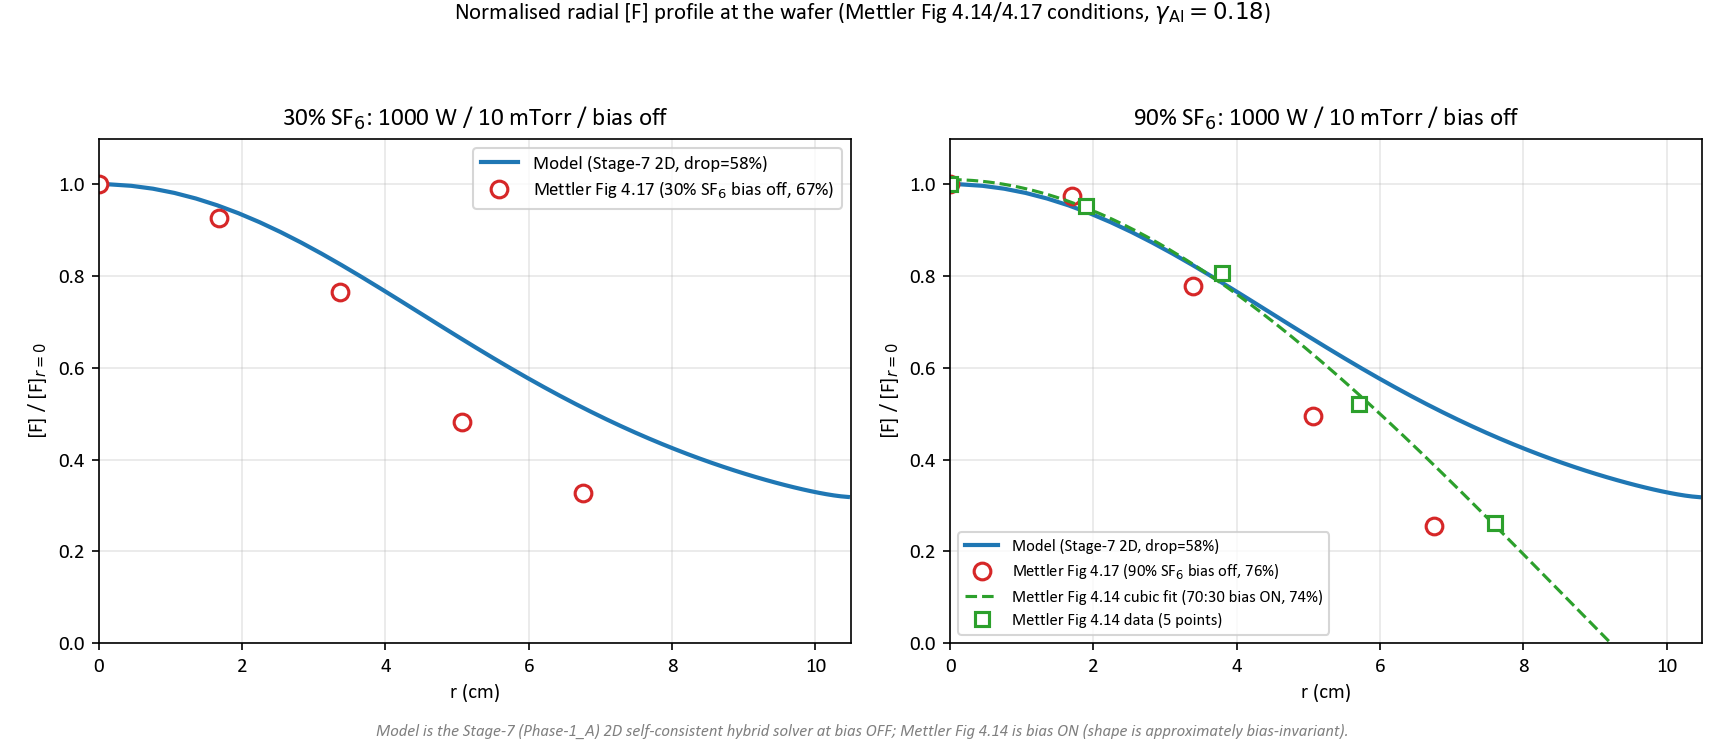
\includegraphics[width=0.95\textwidth]{fig710_radial_F_1000W_regenerated.png}
\caption{Normalised radial [F] profile at the wafer, extracted from the Stage-7 2D self-consistent hybrid solver at Mettler's radial-wafer condition (\SI{1000}{\watt} / \SI{10}{\milli\torr} / bias off, $\gamma_{\mathrm{Al}} = 0.18$).  Left: 30:70 SF$_6$:Ar vs Mettler Fig~4.17 bias-off data (67\% drop).  Right: 90:10 SF$_6$:Ar vs Mettler Fig~4.17 bias-off (76\% drop), with Mettler's Fig~4.14 cubic fit (\emph{bias on}, 70:30 SF$_6$:Ar, 74\% drop) overlaid for reference.  The normalised shape is approximately bias-invariant, so the cubic-fit shape comparison is defensible even with bias off in the model.  The 2D model captures the qualitative radial trend but underpredicts the drop magnitude at 90\%-SF$_6$ by $\sim$18 percentage points, visible in the right panel.  This deficit motivates the electronegative-ambipolar correction listed as Phase-2 deferred item F2 in Section~\ref{sec:future_deferred}.}
\label{fig:future_fig710}
\end{figure}

%======================================================================
\section{Stage 8: Production Packaging}
\label{sec:future_stage8}
%======================================================================

The 2D drift-diffusion model is packaged for production use with a comprehensive test suite (52 automated tests covering unit, integration, and regression levels), parametric sweep capabilities, and mesh convergence verification.  The packaging ensures that the model can be run reliably across the full operating parameter space without manual intervention or case-specific tuning.

%======================================================================
\section{Stage 9: TEL Unified Masked-Domain 2D Model}
\label{sec:future_stage9}
%======================================================================

The TEL reactor's T-shaped geometry is handled through a boolean geometry mask on a $50\times80$ rectangular mesh.  The mask identifies 1669 active (gas-filled) cells and 2331 solid wall cells, with material-specific boundary conditions applied at each gas--wall interface.  This approach avoids the complexity of body-fitted meshes while accurately representing the multi-region reactor architecture.

The electron density profile is prescribed using a Bessel-cosine eigenmode in the ICP source region (capturing the fundamental radial diffusion mode) with exponential decay through the aperture and into the processing chamber.  This profile is consistent with the expected spatial distribution in a high-aspect-ratio ICP source where power deposition is concentrated near the coil.

Material-specific wall recombination probabilities are assigned: $\gamma_\mathrm{Al} = 0.18$ for the aluminium chamber walls (the single calibrated parameter), $\gamma_\mathrm{quartz} = 0.005$ for the quartz ICP tube, and $\gamma_\mathrm{Si} = 0.05$ for the silicon wafer surface.  The $\gamma_\mathrm{Al} = 0.18$ value is calibrated against the \textbf{90:10 SF$_6$:Ar bias-off branch of Mettler Fig~4.17} at \SI{1000}{\watt} / \SI{10}{\milli\torr} (76\% centre-to-edge drop).  Cross-composition validation---specifically the Fig~4.17 30:70 SF$_6$:Ar bias-off branch (67\% drop) and the Fig~4.14 70:30 SF$_6$:Ar bias-\emph{on} condition (74\% cubic-fit drop)---requires additional sweep points and is deferred to Phase-2 work (see Section~\ref{sec:future_deferred}, item F4).  At the calibration condition the model reproduces the 74--76\% drop region; at 30\%-SF$_6$ the Stage-7 run in Figure~\ref{fig:future_fig710} shows a $\sim$10~pp shortfall that quantifies the composition-dependence gap.

%======================================================================
\section{Stage 10: Explicit 0D--2D Hybrid Coupling}
\label{sec:future_stage10}
%======================================================================

The culmination of the modeling program is the explicit coupling of the 0D global model (Chapters~\ref{ch:sf6ar_gasphase}--\ref{ch:wallchem}) with the 2D neutral transport solver (Stage~9), creating a self-consistent hybrid framework.  Four quantities are exchanged between the two solvers at each coupling iteration:

\begin{enumerate}[nosep]
\item \textbf{Electron temperature} $\Te$: computed by the 0D particle balance and passed to the 2D solver to set spatially uniform rate coefficients.
\item \textbf{Volume-averaged electron density} $\bar{n}_e$: computed by the 0D power balance and used to normalize the prescribed $n_e(r,z)$ profile in the 2D solver.
\item \textbf{Electronegativity} $\alpha$: computed from the 0D attachment--recombination balance and used to modify the ambipolar diffusion coefficient in the 2D solver.
\item \textbf{Volume-averaged SF$_6$ density} $\bar{n}_{\mathrm{SF}_6}$: returned from the 2D solver to the 0D model to update the attachment and dissociation rates.
\end{enumerate}

The coupling uses a fixed-point iteration scheme requiring 60--80 iterations for convergence.  Mathematical consistency between the 0D and 2D representations is established through three proofs: (i) the volume-averaged neutral densities from the 2D solver converge to the 0D values when the spatial profile is uniform; (ii) the spatially integrated wall loss rate from the 2D solver equals the 0D wall loss rate when the $h$-factors are consistent; and (iii) the power balance is satisfied to within 1\% at convergence.

The $\Te$ solution within the 0D particle balance uses Brent bisection, which is robust against the multiple-root structure that can arise in electronegative discharges.

%======================================================================
\section{Deferred Mettler Validations}
\label{sec:future_deferred}
%======================================================================

Several comparisons against Mettler's dataset are beyond the scope of the zero-dimensional Phase-1 framework and require explicit capability extensions in Phase 2.  They are enumerated here for traceability.

\begin{itemize}[nosep]
\item \textbf{F1 --- rf-bias sheath model.}  Mettler Figs~4.13 and~4.17 show that \SI{200}{\watt} rf wafer bias enhances [F] by $\sim$1.6$\times$ (90\% SF$_6$) to $\sim$2.15$\times$ (30\% SF$_6$) at the centre.  Reproducing this requires a capacitive-sheath / ion-bombardment coupling; our ICP-only framework has no bias model.

\item \textbf{F2 --- electronegative ambipolar radial broadening.}  The 67\%--76\% radial drop observed by Mettler is steeper at 90\%-SF$_6$ than the cached Stage-7 run in Figure~\ref{fig:future_fig710} reproduces ($\sim$58\% at $r = \SI{8}{\centi\meter}$).  Closing the gap requires the $(1+\alpha)/(1+\alpha T_-/T_e)$ correction to the ambipolar diffusion coefficient in the 2D solver.

\item \textbf{F3 --- diffusion-limited surface regime.}  Mettler's Fig~4.9 etch-rate saturation at $[F] \gtrsim 1.1\times10^{21}$\,m$^{-3}$ indicates a near-wall boundary layer.  A 1D boundary-layer model for WF$_6$/SiF$_4$ transport would be required to reproduce this.

\item \textbf{F4 --- composition sweep of $\gamma_\mathrm{Al}$.}  The current $\gamma_\mathrm{Al} = 0.18$ calibration is tied to the Fig~4.17 90\%-SF$_6$ bias-off branch.  Validating whether a single $\gamma_\mathrm{Al}$ reproduces Fig~4.17's 30\%-SF$_6$ branch (67\% drop) \emph{and} Fig~4.14's 70:30 bias-on cubic fit (74\% drop) requires an additional $\sim$10 sweep points across $\mathrm{frac\_Ar} \in [0, 0.9]$ at Mettler's \SI{1000}{\watt}/\SI{10}{\milli\torr} condition.

\item \textbf{F5 --- E-to-H mode transition.}  The Picard iteration converges to a single H-mode branch; modelling low-power E-to-H transitions requires an impedance-based power-coupling formulation.

\item \textbf{F6 --- spatial wall temperature.}  The TEL chamber has stainless-steel walls, an aluminium pump port, and a silicon wafer.  A single wall temperature smears the F + F + wall recombination rate; a spatially varying $T_{\mathrm{wall}}$ would refine this.

\item \textbf{V5 --- silicon etch probability.}  Mettler Fig~4.18 reports $\varepsilon_{\mathrm{Si}} \approx 0.025$--$0.04$ using locally resolved [F] (flux-independent); actinometry-derived values scatter from 0.05 to 0.10.  Citing these supports the scientific quality of Mettler's probe data but cannot be directly predicted without a Si-etching surface kinetic model.

\item \textbf{Figs 4.12 and 4.16 --- kinetic sanity checks.}  Mettler's W etch probability calibration (Fig~4.12) and Arrhenius activation energy ($E_a = \SI{0.068}{\electronvolt}$, Fig~4.16) underlie the probe-to-density conversion.  Citing these strengthens the case that Mettler's absolute [F] values are calibrated independently of the chemistry being benchmarked.
\end{itemize}

%======================================================================
\section{Roadmap Summary}
\label{sec:future_roadmap}
%======================================================================

The progression from 0D (this report) through 2D drift-diffusion to the coupled 0D--2D hybrid represents a systematic increase in physical fidelity while retaining computational tractability.  The 0D model provides the validated chemistry, surface reactions, and parametric understanding; the 2D model adds spatial resolution for etch uniformity prediction; and the hybrid coupling ensures self-consistency between the two representations.  The full framework executes in under one minute on a single CPU core, enabling the parametric studies and machine-learning surrogate model training that are essential for industrial process optimization.


%=============================================================================
\chapter{Conclusions}
\label{ch:conclusions}
%=============================================================================

%======================================================================
\section{Key Findings}
\label{sec:conc_findings}
%======================================================================

\begin{enumerate}
\item Pressure-dependent neutral recombination (Troe fall-off) is critical at $\lesssim$\SI{20}{\milli\torr}; high-pressure-limit rates overestimate recombination by factors of 5--180.

\item Penning ionisation and Ar$^*$ quenching by molecular species are important for predicting the gradual EN$\to$EP transition with Ar dilution.

\item Wall surface chemistry reduces the $\alpha$ SSE by a factor of 26, resolving the structural over-dissociation error at intermediate Ar fractions.

\item Only 0.7\% of the Kokkoris~\cite{Kokkoris2009} probabilities are required for the stainless-steel Lallement reactor, reflecting wall material and geometry differences.

\item The stiff $\alpha$ transition at ${\sim}67\%$ Ar is a wall chemistry buffer exhaustion threshold, not a numerical artefact.  The root-cause parameter is $s_\mathrm{F}$ (F adsorption probability), which controls $\theta_\mathrm{F}$ feeding the dominant Eley--Rideal SF$_6$ regeneration channel.

\item The kink locus mapped across 35 conditions shows: higher power $\to$ lower kink Ar\%; higher pressure $\to$ higher kink Ar\%.

\item $\eta$ primarily shifts density magnitudes without changing trend shapes, confirming the TEL benchmarking discrepancy is dominated by $\eta$ uncertainty.

\item The model predicts a non-monotonic [F] vs Ar fraction dependence with a maximum at ${\sim}40$--$50\%$ Ar.
\end{enumerate}

%======================================================================
\section{Remaining Gaps}
\label{sec:conc_gaps}
%======================================================================

\begin{itemize}[nosep]
\item \textbf{$\eta_\mathrm{TEL}$:} The single largest obstacle for cross-reactor transferability.  Requires independent $n_e$ measurement.
\item \textbf{$\alpha$ at \SI{5}{\milli\torr}:} Overpredicted by ${\sim}3$--$5\times$.  Lee--Lieberman $h$-factors may lose accuracy at this pressure.
\item \textbf{$\alpha$ above ${\sim}67\%$ Ar:} Unreliable due to the buffer exhaustion transition amplifying surface probability uncertainties.
\item \textbf{TEL wall material:} Wall chemistry probabilities need reactor-specific recalibration.
\item \textbf{Spatial transport:} 0D model cannot capture the ${\sim}\SI{10}{\centi\meter}$ ICP-to-wafer gap in the TEL.
\end{itemize}

%======================================================================
\section{Outlook}
\label{sec:conc_outlook}
%======================================================================

The zero-dimensional global model developed in this report provides a comprehensive and validated foundation for understanding SF$_6$/Ar ICP plasma chemistry.  The model successfully reproduces the principal observables from two independent reference models (Kokkoris et al.~\cite{Kokkoris2009} and Lallement et al.~\cite{Lallement2009}) and demonstrates agreement with spatially resolved experimental measurements~\cite{Mettler2025} when operating conditions match the calibration regime.  The identification of wall chemistry buffer exhaustion as the mechanism driving the stiff electronegativity transition provides new physical insight into the coupling between surface and gas-phase processes in electronegative discharges.

The path forward lies in the spatially resolved modeling framework outlined in Chapter~\ref{ch:future}, which extends the validated 0D chemistry and surface reactions to two-dimensional axisymmetric domains with self-consistent coupling between electromagnetic fields, electron kinetics, and neutral transport.  An independent measurement of the TEL power coupling efficiency would resolve the single largest remaining uncertainty and enable quantitative etch uniformity prediction.


%=============================================================================
\appendix
%=============================================================================

%=============================================================================
\chapter{Data Extraction and Refinement}
\label{app:data}
%=============================================================================

%======================================================================
\section{WebPlotDigitizer Extraction}
\label{sec:app_wpd}
%======================================================================

All reference data were digitised from published figures using WebPlotDigitizer with calibrated axes, yielding 30--60 digitized points per curve.  For curves with overlapping lines (common in multi-species plots), manual refinement was applied to smooth extraction artefacts.

%======================================================================
\section{Refinement Pipeline}
\label{sec:app_refinement}
%======================================================================

The refinement pipeline consists of:
\begin{enumerate}[nosep]
\item Sorting by ascending independent variable and removing duplicates.
\item Identification and removal of outlier points that deviate from the local trend by more than 3\% in log space.
\item Trimming of low-pressure extraction artifacts where identified.
\item Savitzky--Golay smoothing in log space for density quantities, or manual reconstruction from anchor points where artefacts were severe.
\end{enumerate}

The refinement does not bias the benchmark data toward the model predictions.  The smoothing preserves the overall trend, magnitude, and curvature of each digitized curve; it only removes high-frequency noise that is demonstrably absent in the published figures.  Raw and refined datasets are archived separately.

The refinement validation is shown in Figure~\ref{fig:rawvsrefined} (Chapter~\ref{ch:pure_sf6}).

%======================================================================
\section{Reproduction Quality Figures}
\label{sec:app_reproduction}
%======================================================================

\begin{figure}[H]
\centering
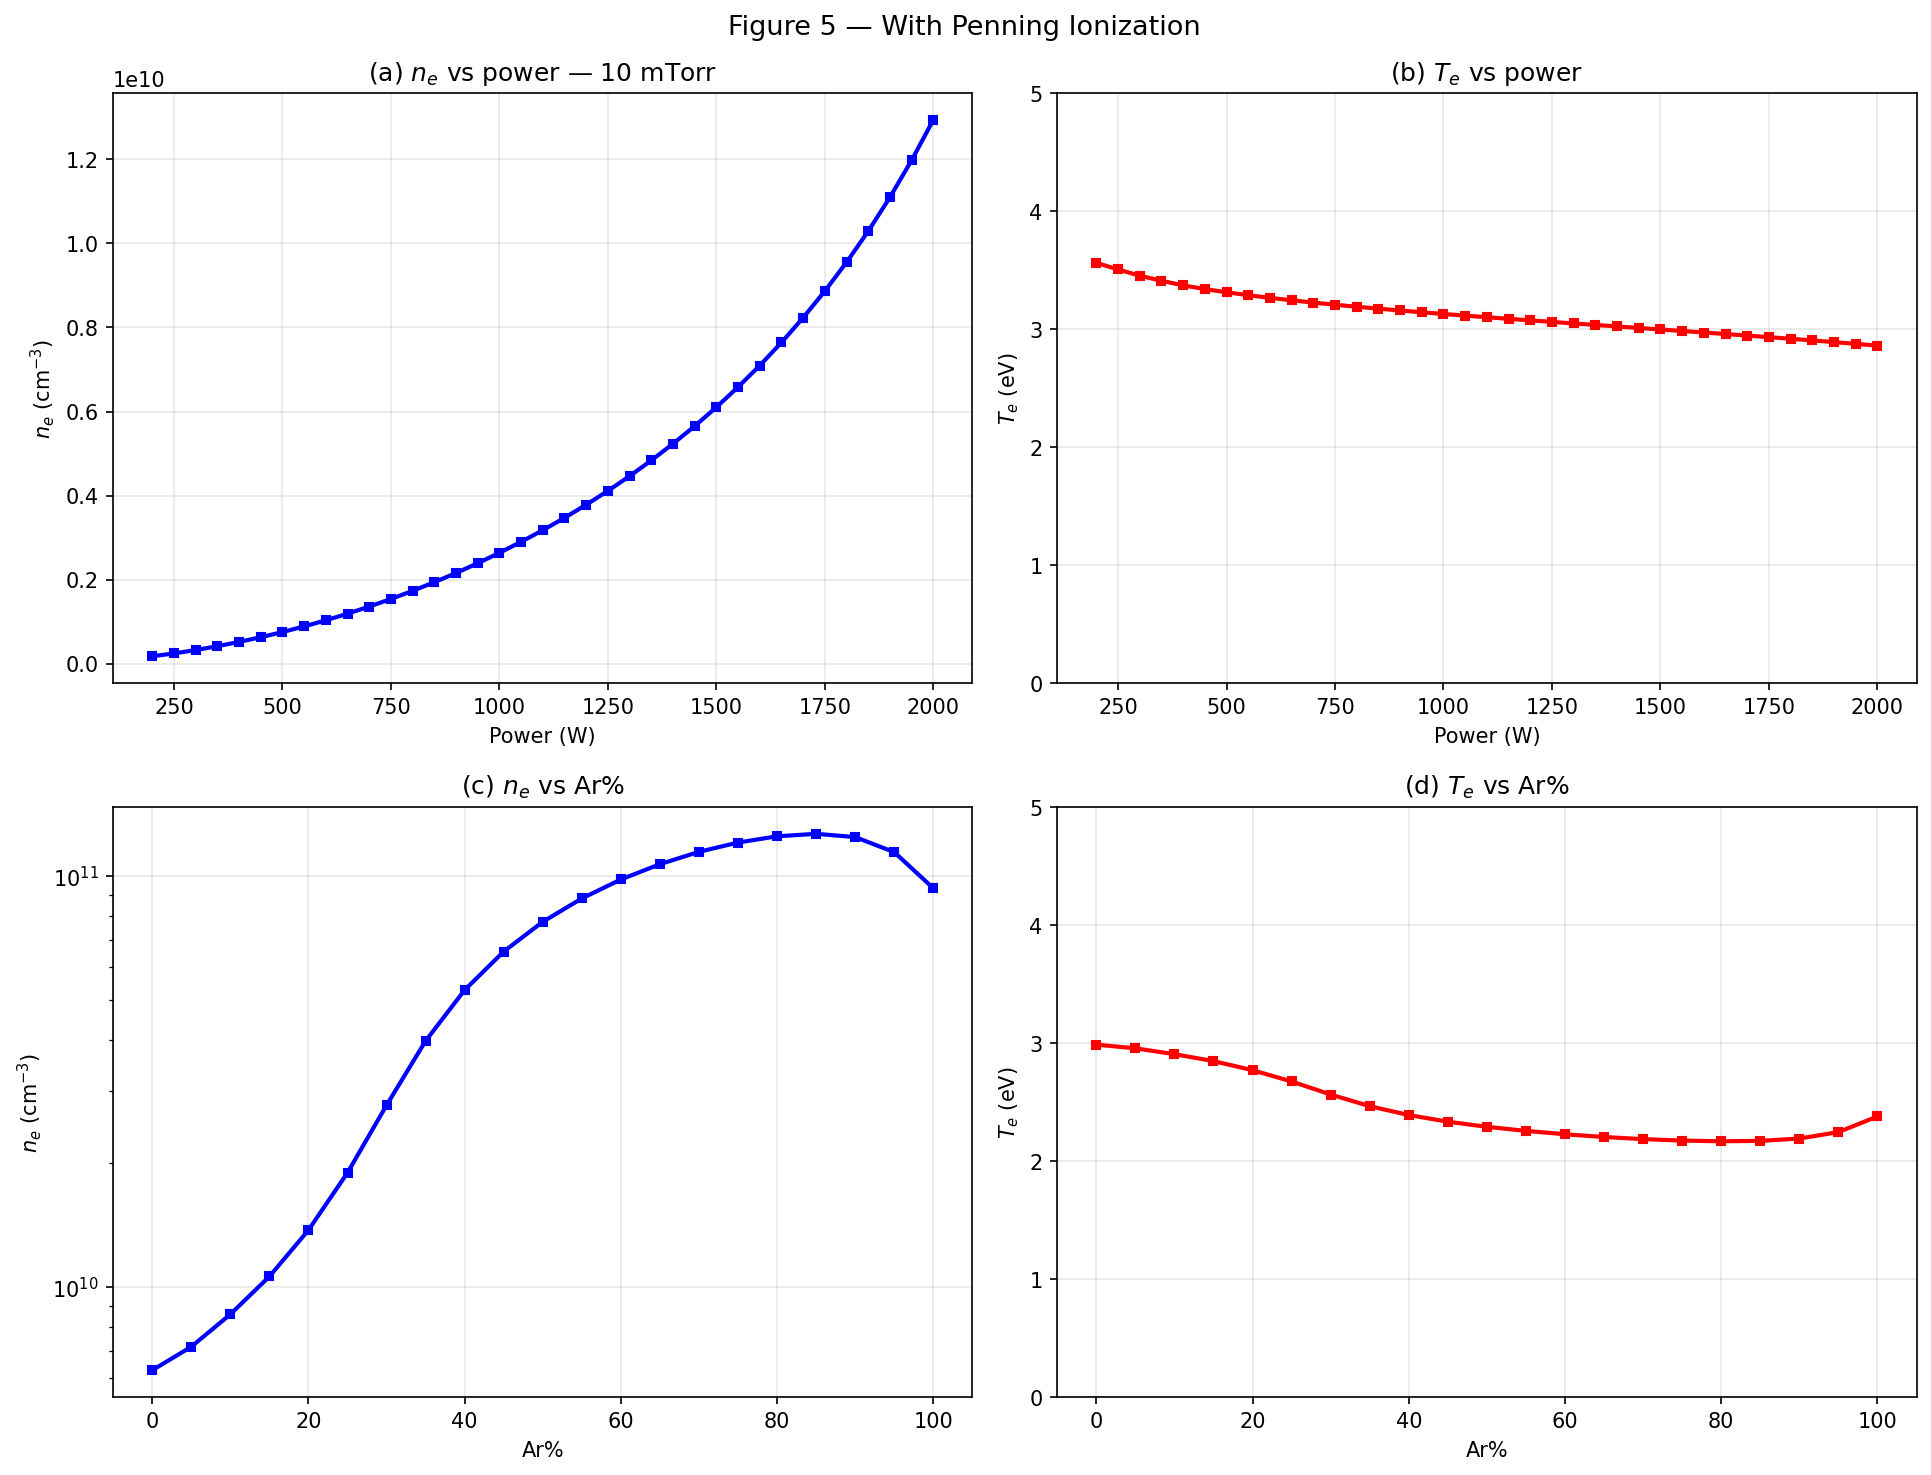
\includegraphics[width=\textwidth]{fig5_reproduction.png}
\caption{Model-only reproduction of Lallement Fig~5: $n_e$ and $\Te$ vs power (top) and Ar fraction (bottom) at \SI{1500}{\watt}, \SI{10}{\milli\torr}.  No reference data overlaid.}
\label{fig:app_fig5_repro}
\end{figure}

\begin{figure}[H]
\centering
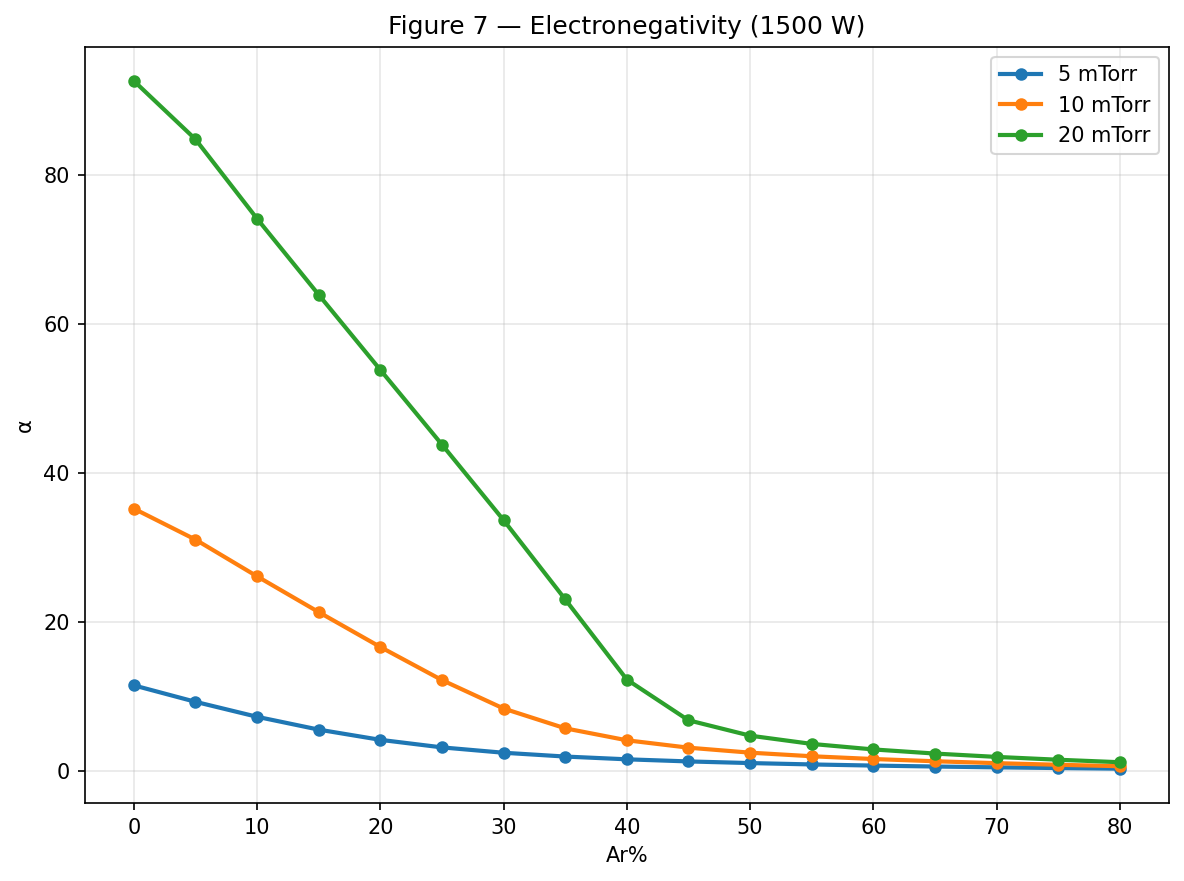
\includegraphics[width=0.85\textwidth]{fig7_reproduction.png}
\caption{Model-only reproduction of Lallement Fig~7: $\alpha$ vs Ar fraction at three pressures.  The correct pressure ordering ($\alpha_{20} > \alpha_{10} > \alpha_5$) is captured.}
\label{fig:app_fig7_repro}
\end{figure}

\begin{figure}[H]
\centering
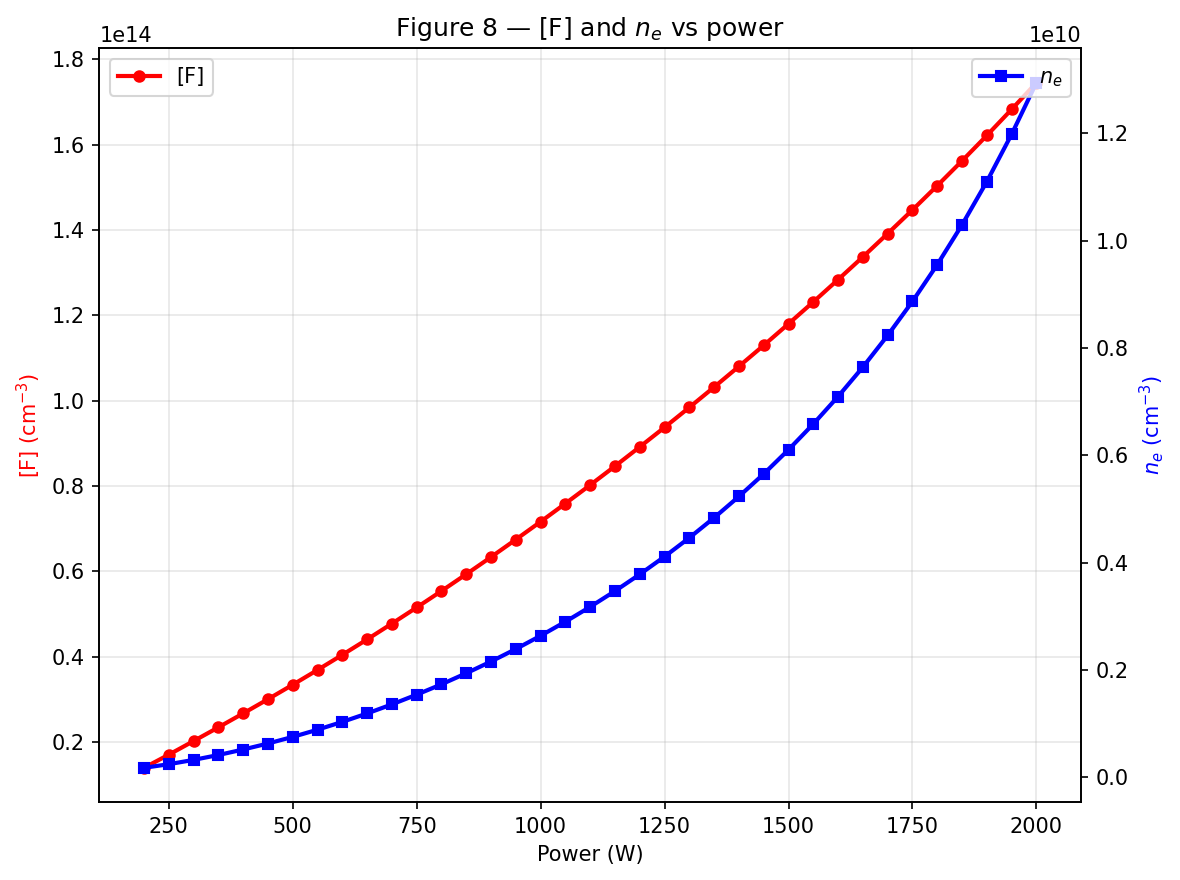
\includegraphics[width=0.85\textwidth]{fig8_reproduction.png}
\caption{Model-only reproduction of Lallement Fig~8: [F] and $n_e$ vs power for pure SF$_6$ at \SI{10}{\milli\torr}.}
\label{fig:app_fig8_repro}
\end{figure}


%=============================================================================
\chapter{Original Paper Figures Used for Digitisation}
\label{app:origfigs}
%=============================================================================

The following figures are screenshots from the Lallement et al.~\cite{Lallement2009} paper, used as source material for the WebPlotDigitizer extraction.  They are included here for reference to allow direct visual comparison with the model reproduction.

\begin{figure}[H]
\centering
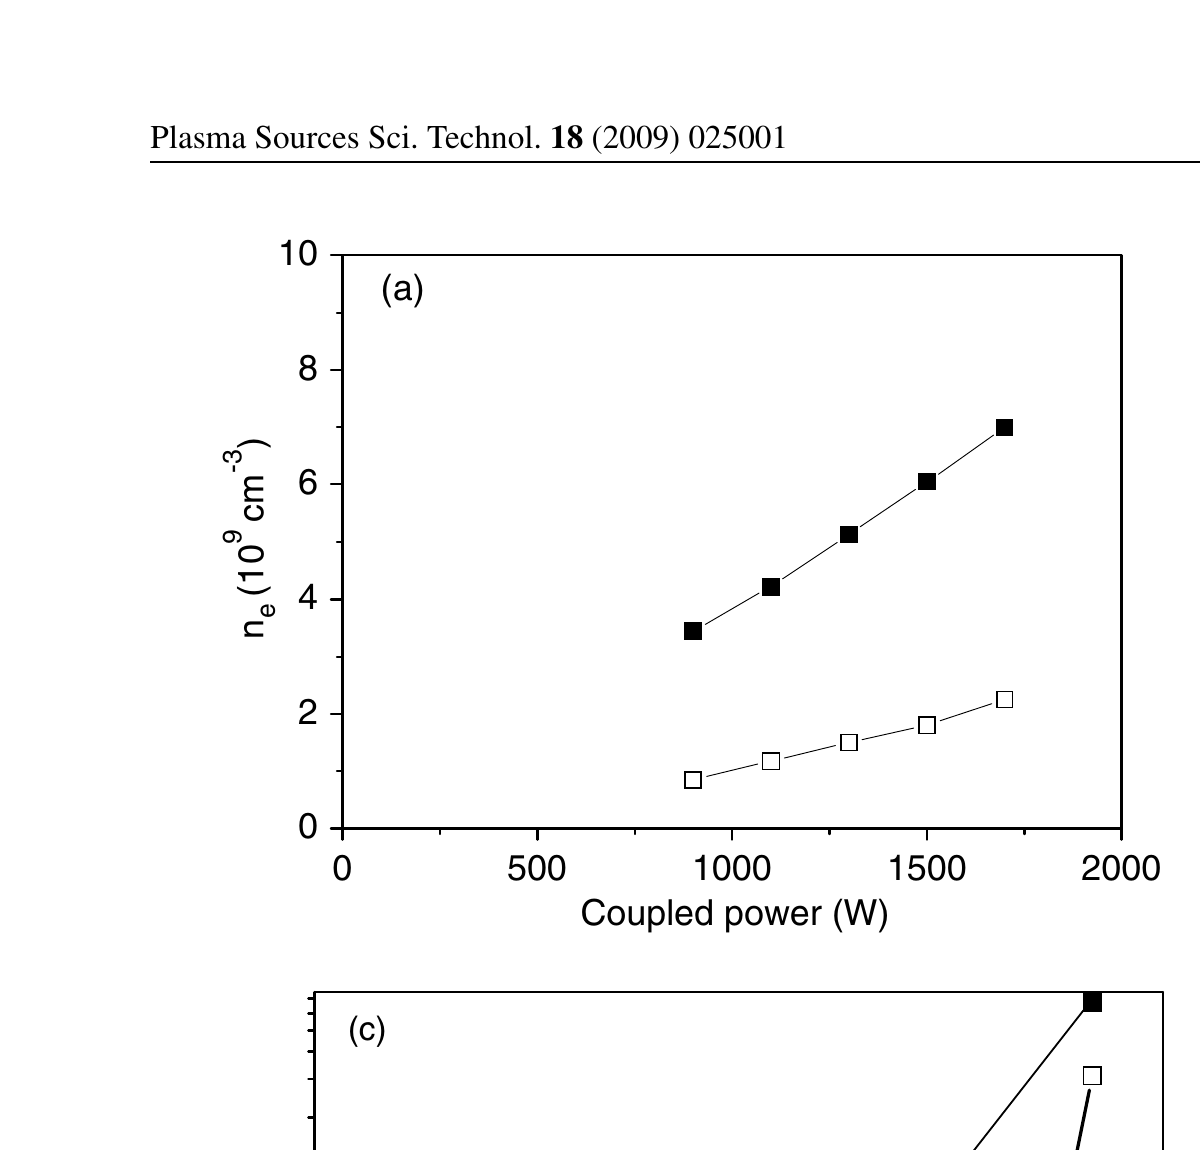
\includegraphics[width=0.48\textwidth]{fig5a_ne_vs_power.png}\hfill
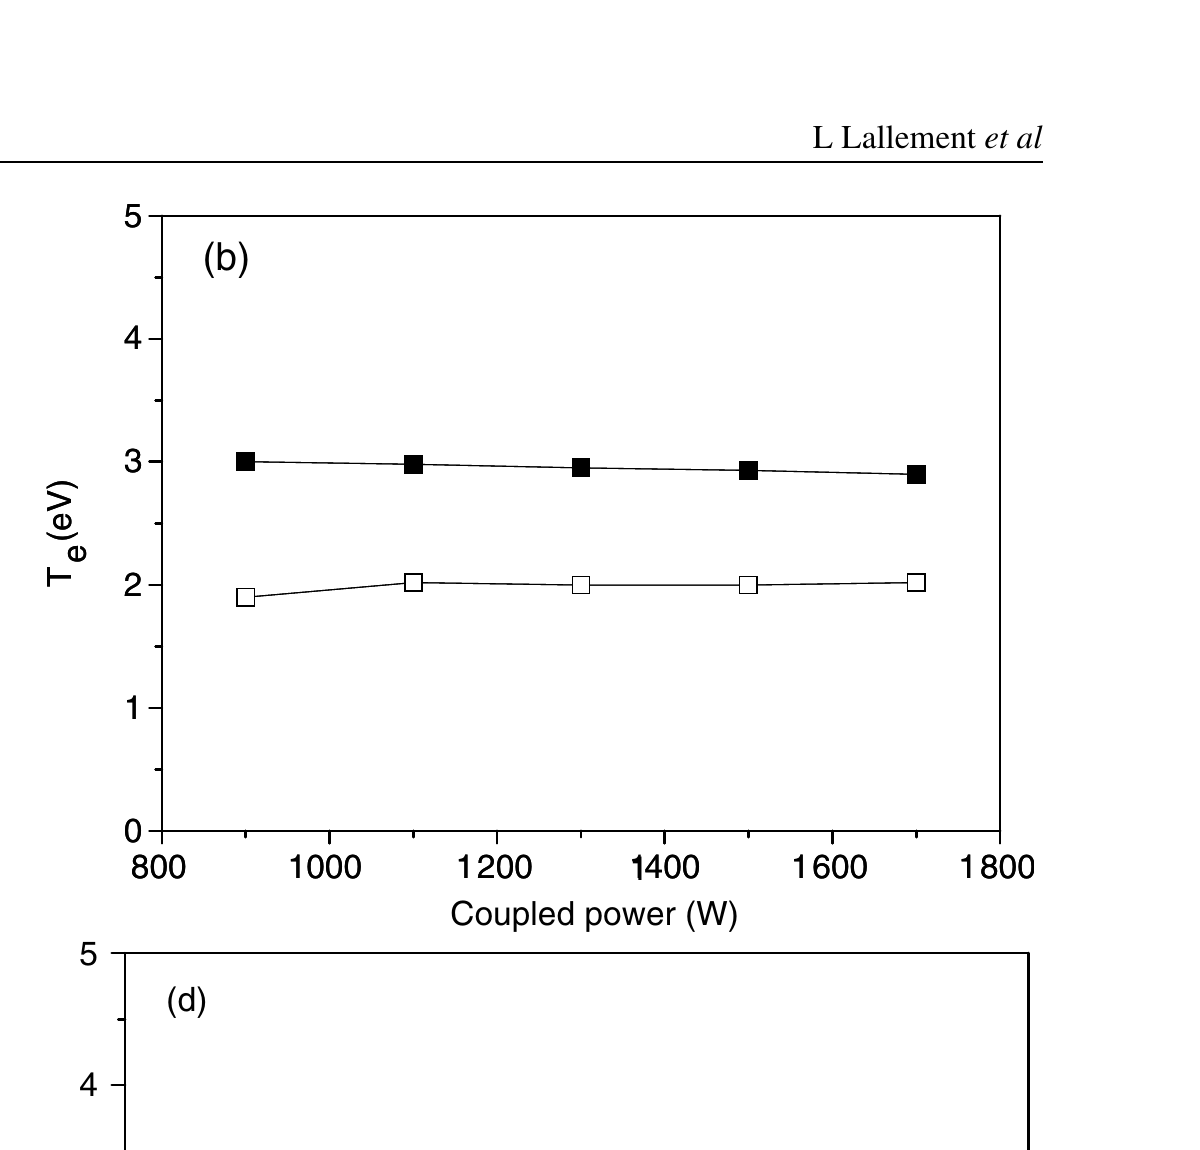
\includegraphics[width=0.48\textwidth]{fig5b_Te_vs_power.png}
\caption{Original Lallement Fig~5(a,b): $n_e$ and $\Te$ vs coupled power for pure SF$_6$ at \SI{10}{\milli\torr}.}
\label{fig:app_orig_fig5ab}
\end{figure}

\begin{figure}[H]
\centering
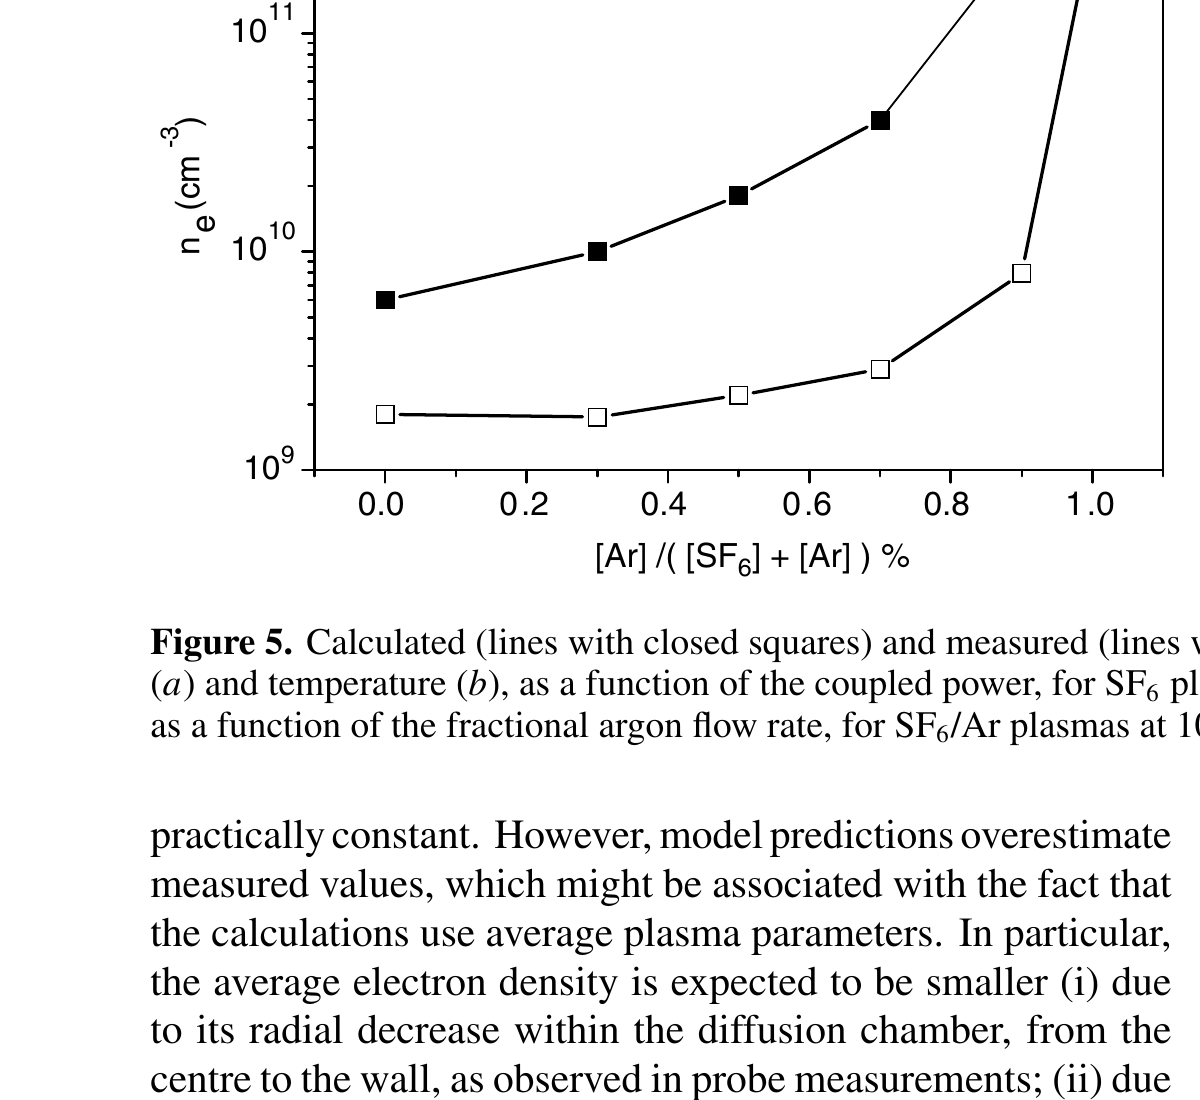
\includegraphics[width=0.48\textwidth]{fig5c_ne_vs_Ar.png}\hfill
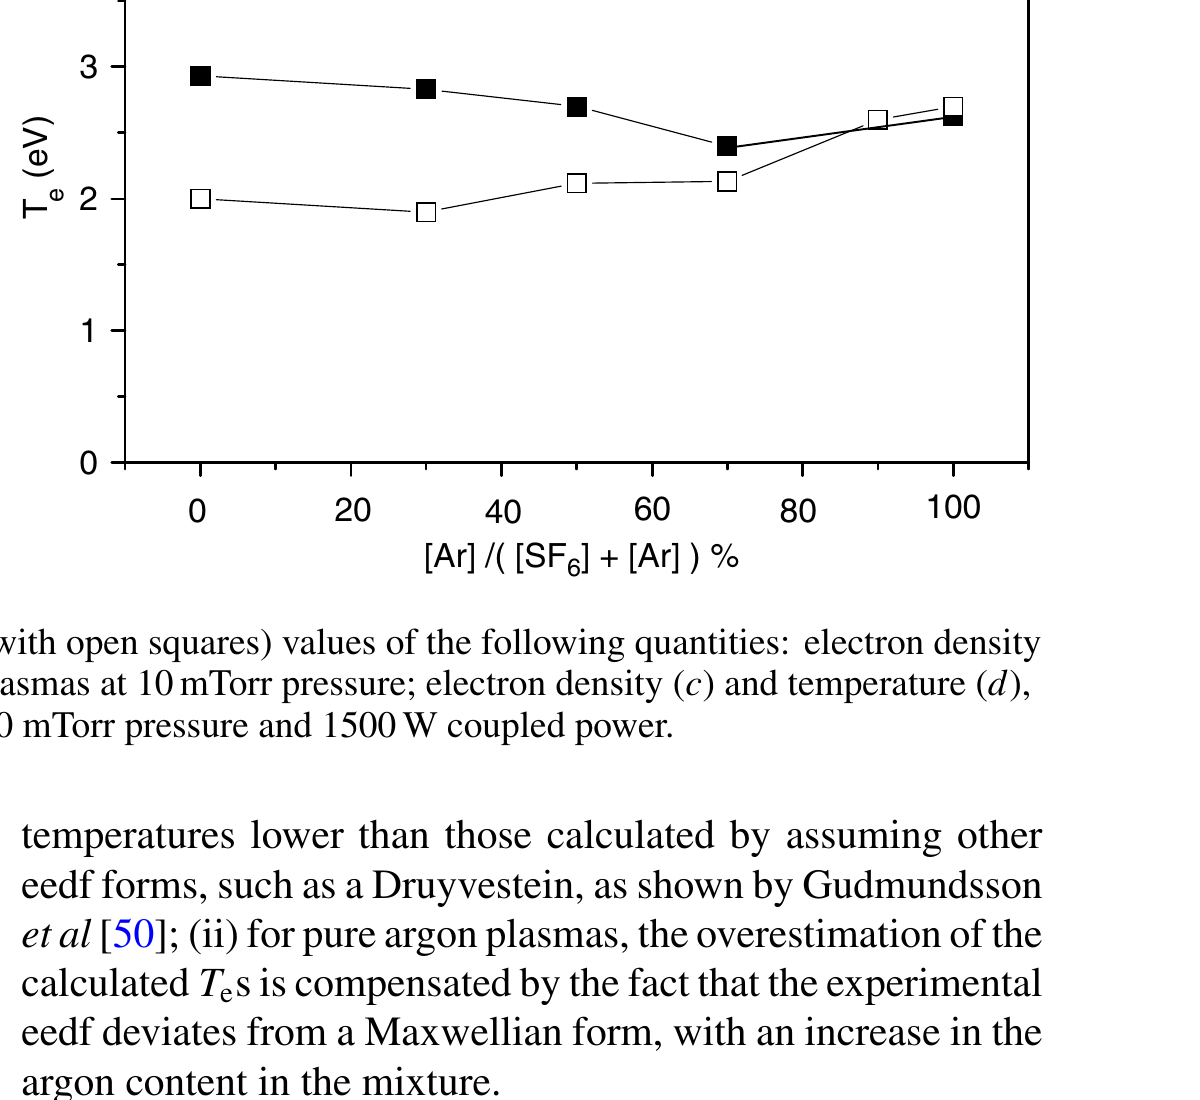
\includegraphics[width=0.48\textwidth]{fig5d_Te_vs_Ar.png}
\caption{Original Lallement Fig~5(c,d): $n_e$ and $\Te$ vs Ar fraction at \SI{1500}{\watt}, \SI{10}{\milli\torr}.}
\label{fig:app_orig_fig5cd}
\end{figure}

\begin{figure}[H]
\centering
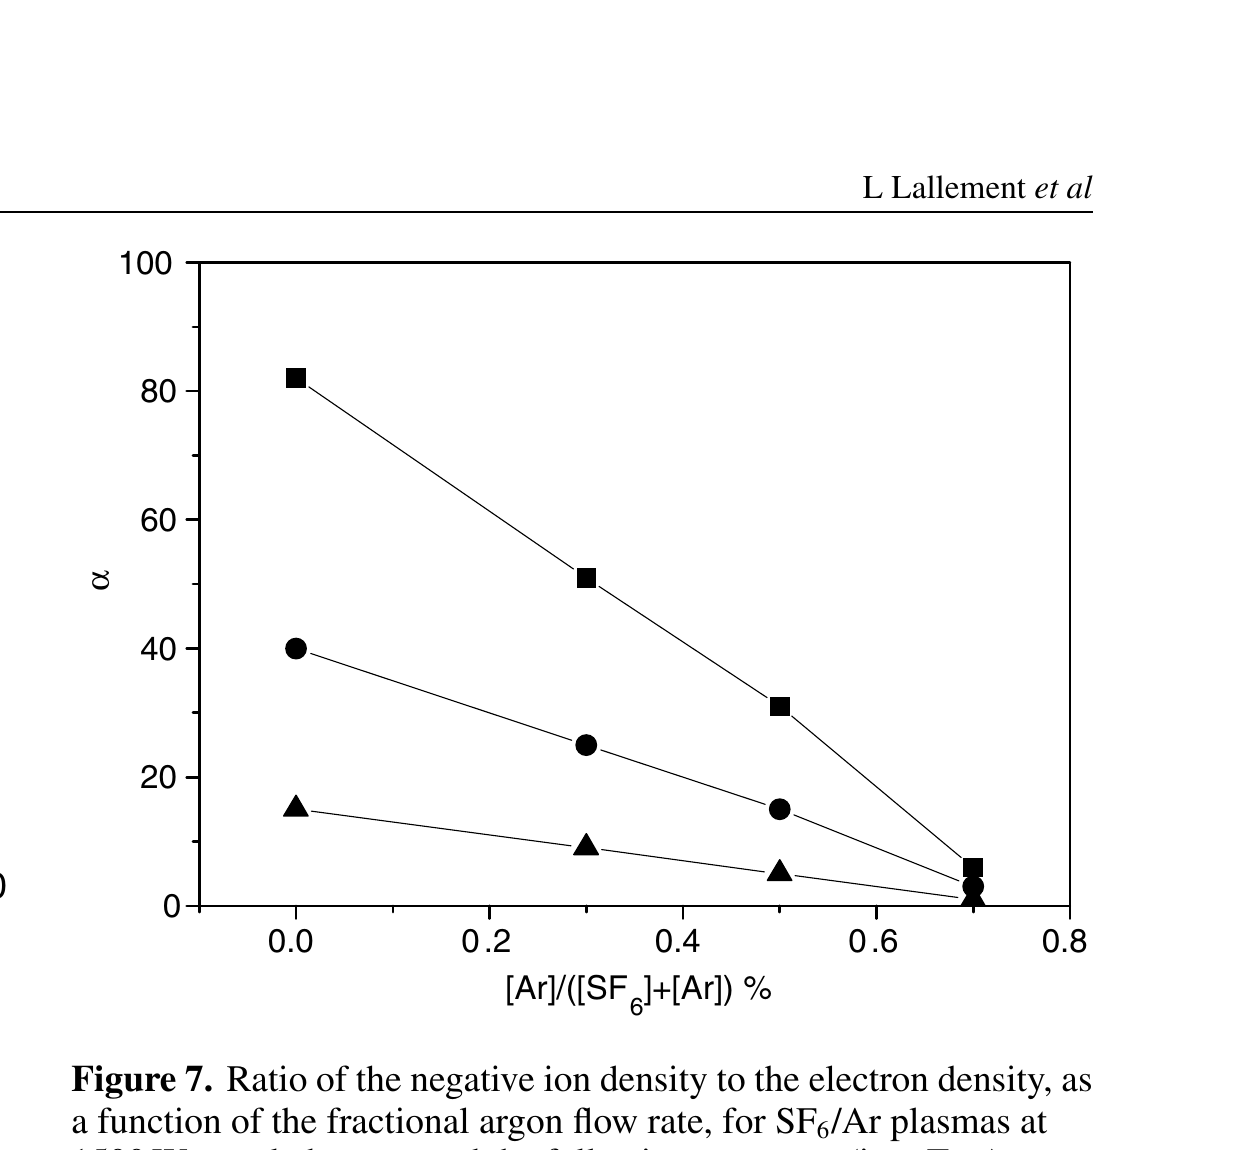
\includegraphics[width=0.48\textwidth]{fig7_alpha_vs_Ar.png}\hfill
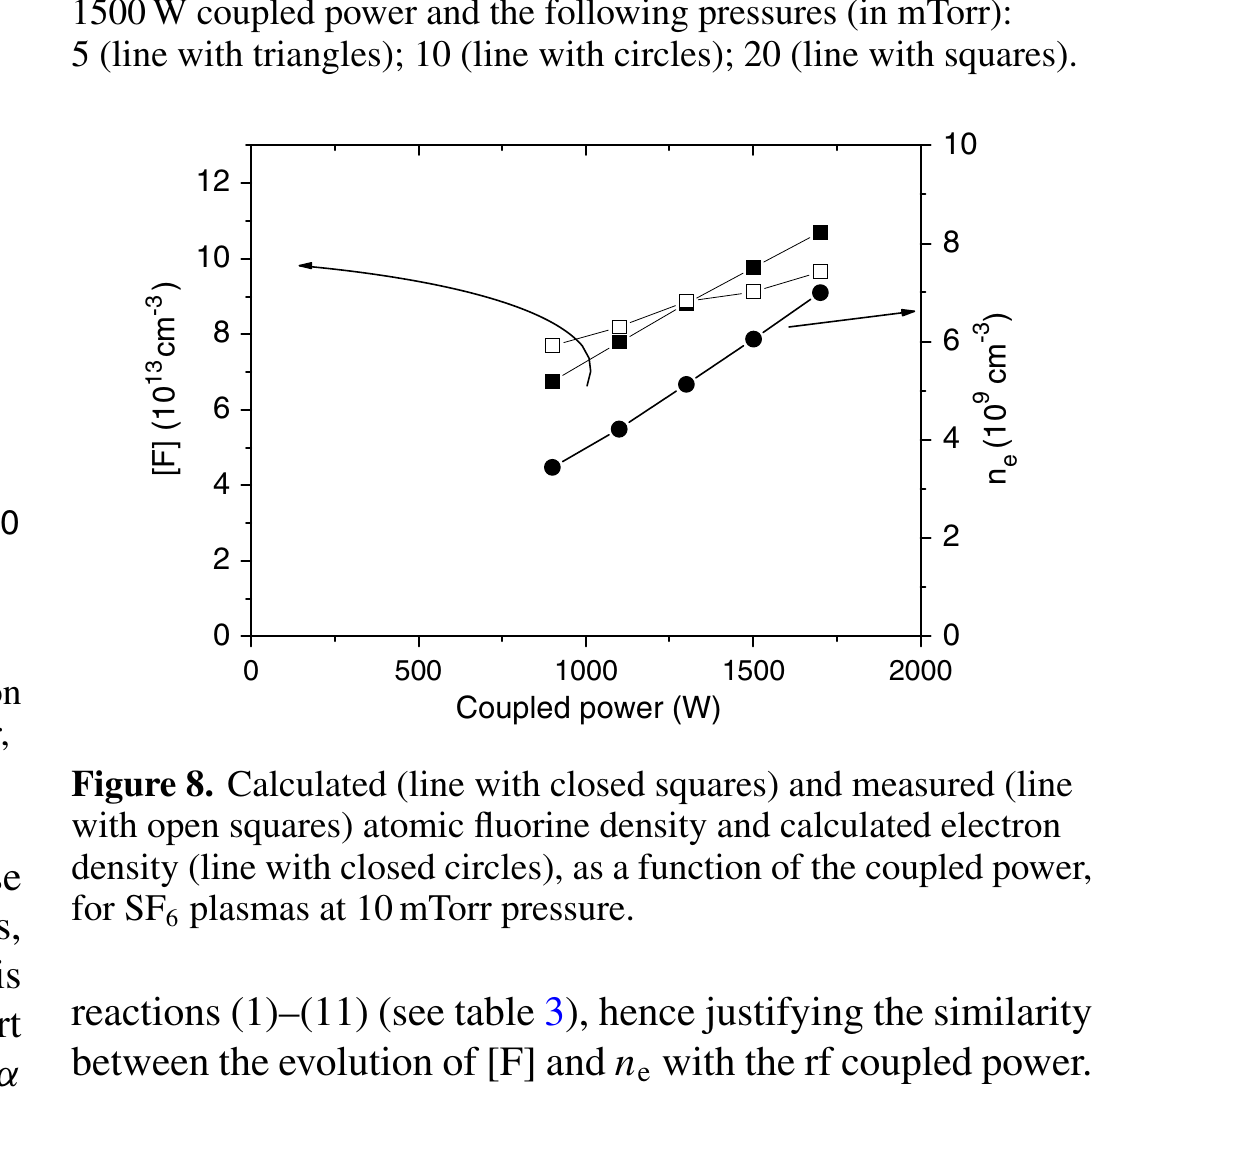
\includegraphics[width=0.48\textwidth]{fig8_F_ne_vs_power.png}
\caption{Original Lallement Fig~7 (left): $\alpha$ vs Ar fraction at three pressures.  Original Fig~8 (right): [F] and $n_e$ vs power for pure SF$_6$ at \SI{10}{\milli\torr}.}
\label{fig:app_orig_fig7_8}
\end{figure}


%=============================================================================
% BIBLIOGRAPHY
%=============================================================================

\bibliographystyle{unsrt}
\bibliography{references}

\end{document}
